\section{Experimental results}
\label{sec:results}

In this section, we explain our implementation of the
presented methods and present quantitative
comparisons for three simulation environments, namely a
holonomic ground robot without and with moving obstacles,
see \cref{fig:point_robot_case}, a robotic manipulator, see
\cref{fig:panda_case}.
Unless stated otherwise, we evaluate 50 cases with different
noise levels $\sigma$. The noisy signal is generated using a
Gaussian distribution centered around the unoisy sensor
data. Specifically, as we use point clouds as inputs to all
presented methods, we have \np{} 3D points to form a
\pointcloud{}. The zero-mean, white noise with variance
$\sigma$ is added to each point to form the noisy
$\pointcloud_{\sigma}$. This noisy sensor data is then used
in the different methods, for computing the \ac{fsd}, the
\ac{sdf}, and no further processing is done for the raw
sensor data.

The performance is measured 
in terms of success, solver time and execution time to reach the goal.
Importantly, the solver time reported in this work does not
include the computation of the environment representation.
For \ac{sdf} however, we included the computation of the
numerical gradient because it is \ac{fabrics}-specific.
Lastly, 
we evaluate the methods in the real world using a
manipulator, see \cref{fig:real_panda},
and a holonomic ground robot, see \cref{fig:real_dingo}.
%
\begin{figure}[ht]
  \begin{subfigure}{0.5\linewidth}
    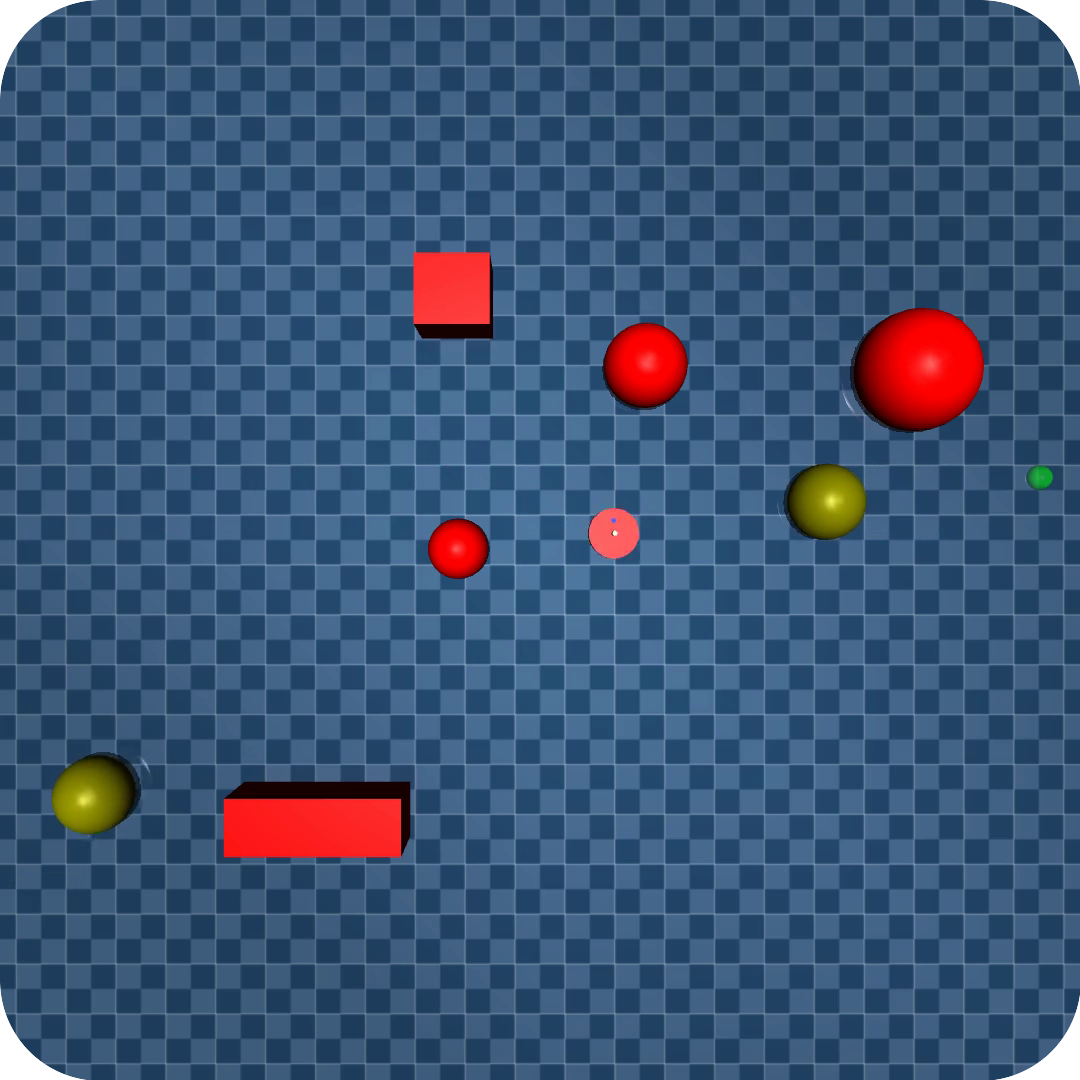
\includegraphics[width=0.95\linewidth]{point_robot_sim/point_robot_dynamic_case.png}
    \caption{Ground robot case}
    \label{fig:point_robot_case}
  \end{subfigure}%
  \begin{subfigure}{0.5\linewidth}
    
\includegraphics[width=0.95\textwidth]{panda_sim/panda_static_case.png}
    \caption{Robotic manipulator case}
    \label{fig:panda_case}
  \end{subfigure}%
  \caption{Simulation cases for the ground robot and the robotic manipulator.}
  \label{fig:simulation_cases}
\end{figure}
%
\begin{figure}[ht]
  \begin{subfigure}{0.5\linewidth}
    \includegraphics[width=0.95\linewidth]{dingo_real/dingo_setup.png}
  \end{subfigure}%
  \begin{subfigure}{0.5\linewidth}
    \includegraphics[width=0.95\linewidth]{dingo_real/dingo.png}
  \end{subfigure}%
  \caption{Real ground robot used to run the experiments.
  For the real-world experiment, we used a Clearpath Dingo
  with a Velodyne VLP16 mounted on top (left). The
  real-world experiment shows the Dingo navigating through
  an environment where a human throws in obstacles (right).
  }
  \label{fig:real_dingo}
\end{figure}
%
\paragraph{Details on implementation}
%
\begin{figure}[ht]
  \centering
  \input{src/24-spahn-ral/img/methods/inkscape/composition_tex.pdf_tex}
  \caption{Composition of symbolic \ac{fabrics} and runtime loop.}
  \label{fig:composition_symbolic_fabrics}
\end{figure}
%
The implementation used in this work uses symbolic
pre-computation of \ac{fabrics}. In this symbolic
interpretation, the composition of the different behaviors
is performed before runtime in a symbolic way, see
\cref{fig:composition_symbolic_fabrics}. The implementation
is identical to the one used
in \cite{spahn2023autotuning}. The code can be found at
\href{www.github.com/tud-amr/fabrics}{Geometric Fabrics}. The simulation
environment as well as the algorithm for computing the \ac{fsd}, \ac{sdf}
and the raw Lidar data can be found as part of
\href{www.github.com/maxspahn/gym_envs_urdf}{urdfenvs}. For the real world
experiments, we used a ROS bridge and used the same
implementation to process the point clouds, generated by
either a Velodyne VLP-16 mounted on the robot, see
\cref{fig:real_dingo}, or by an occupancy grid build using
the octomap package \cite{Hornung2013}.

\subsection{Ground robot}
\label{sub:point_robot}

When comparing explicit environment representations with the proposed techniques
using noise-free sensor data ($\sigma=0.0$), \acp{sdf} demonstrate the highest
success rate. This is likely due to the \textit{guidance} provided by the
\ac{sdf}'s gradient information. Interestingly, the success
rate for an explicit environment representation increases
with the noise level. Potentially, the noisy sensor data is
able to push the robot out of local minima, which were
reported to be a problem for \ac{fabrics} in
\cite{Spahn2023}. The more implicit representations suffer
from the noise increase, most dramatically for the
\ac{sdf} representation, which becomes unusable around a
noise level of $\sigma=0.1$. When exposing all methods to a
dynamic environment (two moving obstacles), the explicit
representation has degrading performance, e.g. without noise 42/50 (static) to
38/50 (dynamic), see
\cref{fig:point_robot_sim_success_dynamic}.
The implicit representations show a similar success rate
across static and dynamic environments.
% static 42,40,38,34
% dynamic 38,42,44,35
Implicit
representations are hardly effected by the dynamic
character. This confirms our hypothesis that implicit
representations are a good approach in human-shared,
changing environments. Moreover, this finding is in line with the findings in
\cite{Spahn2023} on the inability for the explicit
representation to avoid moving obstacles.

The goal reaching times remain similar across all approaches, which aligns with
expectations as the tuning is based on this criterion, as shown in
\cref{subfig:point_robot_sim_metrics}. However, \ac{sdf} and
raw sensor data have some outliers in the time to reach the
goal, which is likely due local minima or
over-conservative behavior in some cases.
While solver computation times are low
for all methods (between $0.5$ ms and $2.0$ ms), utilizing
\ac{sdf} shows the highest computational costs, see
\cref{subfig:point_robot_sim_metrics}. Such low solver
times allow the usage in real-time applications where high
reactivity is required.
%
\begin{figure*}[ht]
  \centering
  %% Creator: Matplotlib, PGF backend
%%
%% To include the figure in your LaTeX document, write
%%   \input{<filename>.pgf}
%%
%% Make sure the required packages are loaded in your preamble
%%   \usepackage{pgf}
%%
%% Also ensure that all the required font packages are loaded; for instance,
%% the lmodern package is sometimes necessary when using math font.
%%   \usepackage{lmodern}
%%
%% Figures using additional raster images can only be included by \input if
%% they are in the same directory as the main LaTeX file. For loading figures
%% from other directories you can use the `import` package
%%   \usepackage{import}
%%
%% and then include the figures with
%%   \import{<path to file>}{<filename>.pgf}
%%
%% Matplotlib used the following preamble
%%   
%%   \makeatletter\@ifpackageloaded{underscore}{}{\usepackage[strings]{underscore}}\makeatother
%%
\begingroup%
\makeatletter%
\begin{pgfpicture}%
\pgfpathrectangle{\pgfpointorigin}{\pgfqpoint{5.220660in}{2.000000in}}%
\pgfusepath{use as bounding box, clip}%
\begin{pgfscope}%
\pgfsetbuttcap%
\pgfsetmiterjoin%
\definecolor{currentfill}{rgb}{1.000000,1.000000,1.000000}%
\pgfsetfillcolor{currentfill}%
\pgfsetlinewidth{0.000000pt}%
\definecolor{currentstroke}{rgb}{1.000000,1.000000,1.000000}%
\pgfsetstrokecolor{currentstroke}%
\pgfsetdash{}{0pt}%
\pgfpathmoveto{\pgfqpoint{0.000000in}{0.000000in}}%
\pgfpathlineto{\pgfqpoint{5.220660in}{0.000000in}}%
\pgfpathlineto{\pgfqpoint{5.220660in}{2.000000in}}%
\pgfpathlineto{\pgfqpoint{0.000000in}{2.000000in}}%
\pgfpathlineto{\pgfqpoint{0.000000in}{0.000000in}}%
\pgfpathclose%
\pgfusepath{fill}%
\end{pgfscope}%
\begin{pgfscope}%
\pgfsetbuttcap%
\pgfsetmiterjoin%
\definecolor{currentfill}{rgb}{1.000000,1.000000,1.000000}%
\pgfsetfillcolor{currentfill}%
\pgfsetlinewidth{0.000000pt}%
\definecolor{currentstroke}{rgb}{0.000000,0.000000,0.000000}%
\pgfsetstrokecolor{currentstroke}%
\pgfsetstrokeopacity{0.000000}%
\pgfsetdash{}{0pt}%
\pgfpathmoveto{\pgfqpoint{0.652582in}{0.400000in}}%
\pgfpathlineto{\pgfqpoint{4.698594in}{0.400000in}}%
\pgfpathlineto{\pgfqpoint{4.698594in}{1.760000in}}%
\pgfpathlineto{\pgfqpoint{0.652582in}{1.760000in}}%
\pgfpathlineto{\pgfqpoint{0.652582in}{0.400000in}}%
\pgfpathclose%
\pgfusepath{fill}%
\end{pgfscope}%
\begin{pgfscope}%
\pgfsetbuttcap%
\pgfsetmiterjoin%
\definecolor{currentfill}{rgb}{1.000000,1.000000,1.000000}%
\pgfsetfillcolor{currentfill}%
\pgfsetlinewidth{0.000000pt}%
\definecolor{currentstroke}{rgb}{0.000000,0.000000,0.000000}%
\pgfsetstrokecolor{currentstroke}%
\pgfsetstrokeopacity{0.000000}%
\pgfsetdash{}{0pt}%
\pgfpathmoveto{\pgfqpoint{0.652582in}{1.760000in}}%
\pgfpathlineto{\pgfqpoint{4.698594in}{1.760000in}}%
\pgfpathlineto{\pgfqpoint{4.698594in}{1.760000in}}%
\pgfpathlineto{\pgfqpoint{0.652582in}{1.760000in}}%
\pgfpathlineto{\pgfqpoint{0.652582in}{1.760000in}}%
\pgfpathclose%
\pgfusepath{fill}%
\end{pgfscope}%
\begin{pgfscope}%
\definecolor{textcolor}{rgb}{0.000000,0.000000,0.000000}%
\pgfsetstrokecolor{textcolor}%
\pgfsetfillcolor{textcolor}%
\pgftext[x=1.184429in,y=1.808611in,,bottom]{\color{textcolor}\rmfamily\fontsize{11.000000}{13.200000}\selectfont explicit}%
\end{pgfscope}%
\begin{pgfscope}%
\definecolor{textcolor}{rgb}{0.000000,0.000000,0.000000}%
\pgfsetstrokecolor{textcolor}%
\pgfsetfillcolor{textcolor}%
\pgftext[x=2.178535in,y=1.808611in,,bottom]{\color{textcolor}\rmfamily\fontsize{11.000000}{13.200000}\selectfont SDF}%
\end{pgfscope}%
\begin{pgfscope}%
\definecolor{textcolor}{rgb}{0.000000,0.000000,0.000000}%
\pgfsetstrokecolor{textcolor}%
\pgfsetfillcolor{textcolor}%
\pgftext[x=3.172641in,y=1.808611in,,bottom]{\color{textcolor}\rmfamily\fontsize{11.000000}{13.200000}\selectfont FSD}%
\end{pgfscope}%
\begin{pgfscope}%
\definecolor{textcolor}{rgb}{0.000000,0.000000,0.000000}%
\pgfsetstrokecolor{textcolor}%
\pgfsetfillcolor{textcolor}%
\pgftext[x=4.166747in,y=1.808611in,,bottom]{\color{textcolor}\rmfamily\fontsize{11.000000}{13.200000}\selectfont Raw}%
\end{pgfscope}%
\begin{pgfscope}%
\pgfpathrectangle{\pgfqpoint{0.652582in}{0.400000in}}{\pgfqpoint{4.046011in}{1.360000in}}%
\pgfusepath{clip}%
\pgfsetbuttcap%
\pgfsetmiterjoin%
\definecolor{currentfill}{rgb}{0.243137,0.647059,0.482353}%
\pgfsetfillcolor{currentfill}%
\pgfsetlinewidth{0.000000pt}%
\definecolor{currentstroke}{rgb}{0.000000,0.000000,0.000000}%
\pgfsetstrokecolor{currentstroke}%
\pgfsetstrokeopacity{0.000000}%
\pgfsetdash{}{0pt}%
\pgfpathmoveto{\pgfqpoint{0.836492in}{0.400000in}}%
\pgfpathlineto{\pgfqpoint{1.035313in}{0.400000in}}%
\pgfpathlineto{\pgfqpoint{1.035313in}{1.542400in}}%
\pgfpathlineto{\pgfqpoint{0.836492in}{1.542400in}}%
\pgfpathlineto{\pgfqpoint{0.836492in}{0.400000in}}%
\pgfpathclose%
\pgfusepath{fill}%
\end{pgfscope}%
\begin{pgfscope}%
\pgfpathrectangle{\pgfqpoint{0.652582in}{0.400000in}}{\pgfqpoint{4.046011in}{1.360000in}}%
\pgfusepath{clip}%
\pgfsetbuttcap%
\pgfsetmiterjoin%
\definecolor{currentfill}{rgb}{0.243137,0.647059,0.482353}%
\pgfsetfillcolor{currentfill}%
\pgfsetlinewidth{0.000000pt}%
\definecolor{currentstroke}{rgb}{0.000000,0.000000,0.000000}%
\pgfsetstrokecolor{currentstroke}%
\pgfsetstrokeopacity{0.000000}%
\pgfsetdash{}{0pt}%
\pgfpathmoveto{\pgfqpoint{1.830598in}{0.400000in}}%
\pgfpathlineto{\pgfqpoint{2.029419in}{0.400000in}}%
\pgfpathlineto{\pgfqpoint{2.029419in}{1.488000in}}%
\pgfpathlineto{\pgfqpoint{1.830598in}{1.488000in}}%
\pgfpathlineto{\pgfqpoint{1.830598in}{0.400000in}}%
\pgfpathclose%
\pgfusepath{fill}%
\end{pgfscope}%
\begin{pgfscope}%
\pgfpathrectangle{\pgfqpoint{0.652582in}{0.400000in}}{\pgfqpoint{4.046011in}{1.360000in}}%
\pgfusepath{clip}%
\pgfsetbuttcap%
\pgfsetmiterjoin%
\definecolor{currentfill}{rgb}{0.243137,0.647059,0.482353}%
\pgfsetfillcolor{currentfill}%
\pgfsetlinewidth{0.000000pt}%
\definecolor{currentstroke}{rgb}{0.000000,0.000000,0.000000}%
\pgfsetstrokecolor{currentstroke}%
\pgfsetstrokeopacity{0.000000}%
\pgfsetdash{}{0pt}%
\pgfpathmoveto{\pgfqpoint{2.824704in}{0.400000in}}%
\pgfpathlineto{\pgfqpoint{3.023525in}{0.400000in}}%
\pgfpathlineto{\pgfqpoint{3.023525in}{1.433600in}}%
\pgfpathlineto{\pgfqpoint{2.824704in}{1.433600in}}%
\pgfpathlineto{\pgfqpoint{2.824704in}{0.400000in}}%
\pgfpathclose%
\pgfusepath{fill}%
\end{pgfscope}%
\begin{pgfscope}%
\pgfpathrectangle{\pgfqpoint{0.652582in}{0.400000in}}{\pgfqpoint{4.046011in}{1.360000in}}%
\pgfusepath{clip}%
\pgfsetbuttcap%
\pgfsetmiterjoin%
\definecolor{currentfill}{rgb}{0.243137,0.647059,0.482353}%
\pgfsetfillcolor{currentfill}%
\pgfsetlinewidth{0.000000pt}%
\definecolor{currentstroke}{rgb}{0.000000,0.000000,0.000000}%
\pgfsetstrokecolor{currentstroke}%
\pgfsetstrokeopacity{0.000000}%
\pgfsetdash{}{0pt}%
\pgfpathmoveto{\pgfqpoint{3.818810in}{0.400000in}}%
\pgfpathlineto{\pgfqpoint{4.017631in}{0.400000in}}%
\pgfpathlineto{\pgfqpoint{4.017631in}{1.324800in}}%
\pgfpathlineto{\pgfqpoint{3.818810in}{1.324800in}}%
\pgfpathlineto{\pgfqpoint{3.818810in}{0.400000in}}%
\pgfpathclose%
\pgfusepath{fill}%
\end{pgfscope}%
\begin{pgfscope}%
\pgfpathrectangle{\pgfqpoint{0.652582in}{0.400000in}}{\pgfqpoint{4.046011in}{1.360000in}}%
\pgfusepath{clip}%
\pgfsetbuttcap%
\pgfsetmiterjoin%
\definecolor{currentfill}{rgb}{0.792157,0.439216,0.505882}%
\pgfsetfillcolor{currentfill}%
\pgfsetlinewidth{0.000000pt}%
\definecolor{currentstroke}{rgb}{0.000000,0.000000,0.000000}%
\pgfsetstrokecolor{currentstroke}%
\pgfsetstrokeopacity{0.000000}%
\pgfsetdash{}{0pt}%
\pgfpathmoveto{\pgfqpoint{0.836492in}{1.542400in}}%
\pgfpathlineto{\pgfqpoint{1.035313in}{1.542400in}}%
\pgfpathlineto{\pgfqpoint{1.035313in}{1.569600in}}%
\pgfpathlineto{\pgfqpoint{0.836492in}{1.569600in}}%
\pgfpathlineto{\pgfqpoint{0.836492in}{1.542400in}}%
\pgfpathclose%
\pgfusepath{fill}%
\end{pgfscope}%
\begin{pgfscope}%
\pgfpathrectangle{\pgfqpoint{0.652582in}{0.400000in}}{\pgfqpoint{4.046011in}{1.360000in}}%
\pgfusepath{clip}%
\pgfsetbuttcap%
\pgfsetmiterjoin%
\definecolor{currentfill}{rgb}{0.792157,0.439216,0.505882}%
\pgfsetfillcolor{currentfill}%
\pgfsetlinewidth{0.000000pt}%
\definecolor{currentstroke}{rgb}{0.000000,0.000000,0.000000}%
\pgfsetstrokecolor{currentstroke}%
\pgfsetstrokeopacity{0.000000}%
\pgfsetdash{}{0pt}%
\pgfpathmoveto{\pgfqpoint{1.830598in}{1.488000in}}%
\pgfpathlineto{\pgfqpoint{2.029419in}{1.488000in}}%
\pgfpathlineto{\pgfqpoint{2.029419in}{1.624000in}}%
\pgfpathlineto{\pgfqpoint{1.830598in}{1.624000in}}%
\pgfpathlineto{\pgfqpoint{1.830598in}{1.488000in}}%
\pgfpathclose%
\pgfusepath{fill}%
\end{pgfscope}%
\begin{pgfscope}%
\pgfpathrectangle{\pgfqpoint{0.652582in}{0.400000in}}{\pgfqpoint{4.046011in}{1.360000in}}%
\pgfusepath{clip}%
\pgfsetbuttcap%
\pgfsetmiterjoin%
\definecolor{currentfill}{rgb}{0.792157,0.439216,0.505882}%
\pgfsetfillcolor{currentfill}%
\pgfsetlinewidth{0.000000pt}%
\definecolor{currentstroke}{rgb}{0.000000,0.000000,0.000000}%
\pgfsetstrokecolor{currentstroke}%
\pgfsetstrokeopacity{0.000000}%
\pgfsetdash{}{0pt}%
\pgfpathmoveto{\pgfqpoint{2.824704in}{1.433600in}}%
\pgfpathlineto{\pgfqpoint{3.023525in}{1.433600in}}%
\pgfpathlineto{\pgfqpoint{3.023525in}{1.624000in}}%
\pgfpathlineto{\pgfqpoint{2.824704in}{1.624000in}}%
\pgfpathlineto{\pgfqpoint{2.824704in}{1.433600in}}%
\pgfpathclose%
\pgfusepath{fill}%
\end{pgfscope}%
\begin{pgfscope}%
\pgfpathrectangle{\pgfqpoint{0.652582in}{0.400000in}}{\pgfqpoint{4.046011in}{1.360000in}}%
\pgfusepath{clip}%
\pgfsetbuttcap%
\pgfsetmiterjoin%
\definecolor{currentfill}{rgb}{0.792157,0.439216,0.505882}%
\pgfsetfillcolor{currentfill}%
\pgfsetlinewidth{0.000000pt}%
\definecolor{currentstroke}{rgb}{0.000000,0.000000,0.000000}%
\pgfsetstrokecolor{currentstroke}%
\pgfsetstrokeopacity{0.000000}%
\pgfsetdash{}{0pt}%
\pgfpathmoveto{\pgfqpoint{3.818810in}{1.324800in}}%
\pgfpathlineto{\pgfqpoint{4.017631in}{1.324800in}}%
\pgfpathlineto{\pgfqpoint{4.017631in}{1.324800in}}%
\pgfpathlineto{\pgfqpoint{3.818810in}{1.324800in}}%
\pgfpathlineto{\pgfqpoint{3.818810in}{1.324800in}}%
\pgfpathclose%
\pgfusepath{fill}%
\end{pgfscope}%
\begin{pgfscope}%
\pgfpathrectangle{\pgfqpoint{0.652582in}{0.400000in}}{\pgfqpoint{4.046011in}{1.360000in}}%
\pgfusepath{clip}%
\pgfsetbuttcap%
\pgfsetmiterjoin%
\definecolor{currentfill}{rgb}{0.000000,0.627451,0.729412}%
\pgfsetfillcolor{currentfill}%
\pgfsetlinewidth{0.000000pt}%
\definecolor{currentstroke}{rgb}{0.000000,0.000000,0.000000}%
\pgfsetstrokecolor{currentstroke}%
\pgfsetstrokeopacity{0.000000}%
\pgfsetdash{}{0pt}%
\pgfpathmoveto{\pgfqpoint{0.836492in}{1.569600in}}%
\pgfpathlineto{\pgfqpoint{1.035313in}{1.569600in}}%
\pgfpathlineto{\pgfqpoint{1.035313in}{1.596800in}}%
\pgfpathlineto{\pgfqpoint{0.836492in}{1.596800in}}%
\pgfpathlineto{\pgfqpoint{0.836492in}{1.569600in}}%
\pgfpathclose%
\pgfusepath{fill}%
\end{pgfscope}%
\begin{pgfscope}%
\pgfpathrectangle{\pgfqpoint{0.652582in}{0.400000in}}{\pgfqpoint{4.046011in}{1.360000in}}%
\pgfusepath{clip}%
\pgfsetbuttcap%
\pgfsetmiterjoin%
\definecolor{currentfill}{rgb}{0.000000,0.627451,0.729412}%
\pgfsetfillcolor{currentfill}%
\pgfsetlinewidth{0.000000pt}%
\definecolor{currentstroke}{rgb}{0.000000,0.000000,0.000000}%
\pgfsetstrokecolor{currentstroke}%
\pgfsetstrokeopacity{0.000000}%
\pgfsetdash{}{0pt}%
\pgfpathmoveto{\pgfqpoint{1.830598in}{1.624000in}}%
\pgfpathlineto{\pgfqpoint{2.029419in}{1.624000in}}%
\pgfpathlineto{\pgfqpoint{2.029419in}{1.705600in}}%
\pgfpathlineto{\pgfqpoint{1.830598in}{1.705600in}}%
\pgfpathlineto{\pgfqpoint{1.830598in}{1.624000in}}%
\pgfpathclose%
\pgfusepath{fill}%
\end{pgfscope}%
\begin{pgfscope}%
\pgfpathrectangle{\pgfqpoint{0.652582in}{0.400000in}}{\pgfqpoint{4.046011in}{1.360000in}}%
\pgfusepath{clip}%
\pgfsetbuttcap%
\pgfsetmiterjoin%
\definecolor{currentfill}{rgb}{0.000000,0.627451,0.729412}%
\pgfsetfillcolor{currentfill}%
\pgfsetlinewidth{0.000000pt}%
\definecolor{currentstroke}{rgb}{0.000000,0.000000,0.000000}%
\pgfsetstrokecolor{currentstroke}%
\pgfsetstrokeopacity{0.000000}%
\pgfsetdash{}{0pt}%
\pgfpathmoveto{\pgfqpoint{2.824704in}{1.624000in}}%
\pgfpathlineto{\pgfqpoint{3.023525in}{1.624000in}}%
\pgfpathlineto{\pgfqpoint{3.023525in}{1.678400in}}%
\pgfpathlineto{\pgfqpoint{2.824704in}{1.678400in}}%
\pgfpathlineto{\pgfqpoint{2.824704in}{1.624000in}}%
\pgfpathclose%
\pgfusepath{fill}%
\end{pgfscope}%
\begin{pgfscope}%
\pgfpathrectangle{\pgfqpoint{0.652582in}{0.400000in}}{\pgfqpoint{4.046011in}{1.360000in}}%
\pgfusepath{clip}%
\pgfsetbuttcap%
\pgfsetmiterjoin%
\definecolor{currentfill}{rgb}{0.000000,0.627451,0.729412}%
\pgfsetfillcolor{currentfill}%
\pgfsetlinewidth{0.000000pt}%
\definecolor{currentstroke}{rgb}{0.000000,0.000000,0.000000}%
\pgfsetstrokecolor{currentstroke}%
\pgfsetstrokeopacity{0.000000}%
\pgfsetdash{}{0pt}%
\pgfpathmoveto{\pgfqpoint{3.818810in}{1.324800in}}%
\pgfpathlineto{\pgfqpoint{4.017631in}{1.324800in}}%
\pgfpathlineto{\pgfqpoint{4.017631in}{1.406400in}}%
\pgfpathlineto{\pgfqpoint{3.818810in}{1.406400in}}%
\pgfpathlineto{\pgfqpoint{3.818810in}{1.324800in}}%
\pgfpathclose%
\pgfusepath{fill}%
\end{pgfscope}%
\begin{pgfscope}%
\pgfpathrectangle{\pgfqpoint{0.652582in}{0.400000in}}{\pgfqpoint{4.046011in}{1.360000in}}%
\pgfusepath{clip}%
\pgfsetbuttcap%
\pgfsetmiterjoin%
\definecolor{currentfill}{rgb}{0.760784,0.490196,0.250980}%
\pgfsetfillcolor{currentfill}%
\pgfsetlinewidth{0.000000pt}%
\definecolor{currentstroke}{rgb}{0.000000,0.000000,0.000000}%
\pgfsetstrokecolor{currentstroke}%
\pgfsetstrokeopacity{0.000000}%
\pgfsetdash{}{0pt}%
\pgfpathmoveto{\pgfqpoint{0.836492in}{1.596800in}}%
\pgfpathlineto{\pgfqpoint{1.035313in}{1.596800in}}%
\pgfpathlineto{\pgfqpoint{1.035313in}{1.760000in}}%
\pgfpathlineto{\pgfqpoint{0.836492in}{1.760000in}}%
\pgfpathlineto{\pgfqpoint{0.836492in}{1.596800in}}%
\pgfpathclose%
\pgfusepath{fill}%
\end{pgfscope}%
\begin{pgfscope}%
\pgfpathrectangle{\pgfqpoint{0.652582in}{0.400000in}}{\pgfqpoint{4.046011in}{1.360000in}}%
\pgfusepath{clip}%
\pgfsetbuttcap%
\pgfsetmiterjoin%
\definecolor{currentfill}{rgb}{0.760784,0.490196,0.250980}%
\pgfsetfillcolor{currentfill}%
\pgfsetlinewidth{0.000000pt}%
\definecolor{currentstroke}{rgb}{0.000000,0.000000,0.000000}%
\pgfsetstrokecolor{currentstroke}%
\pgfsetstrokeopacity{0.000000}%
\pgfsetdash{}{0pt}%
\pgfpathmoveto{\pgfqpoint{1.830598in}{1.705600in}}%
\pgfpathlineto{\pgfqpoint{2.029419in}{1.705600in}}%
\pgfpathlineto{\pgfqpoint{2.029419in}{1.760000in}}%
\pgfpathlineto{\pgfqpoint{1.830598in}{1.760000in}}%
\pgfpathlineto{\pgfqpoint{1.830598in}{1.705600in}}%
\pgfpathclose%
\pgfusepath{fill}%
\end{pgfscope}%
\begin{pgfscope}%
\pgfpathrectangle{\pgfqpoint{0.652582in}{0.400000in}}{\pgfqpoint{4.046011in}{1.360000in}}%
\pgfusepath{clip}%
\pgfsetbuttcap%
\pgfsetmiterjoin%
\definecolor{currentfill}{rgb}{0.760784,0.490196,0.250980}%
\pgfsetfillcolor{currentfill}%
\pgfsetlinewidth{0.000000pt}%
\definecolor{currentstroke}{rgb}{0.000000,0.000000,0.000000}%
\pgfsetstrokecolor{currentstroke}%
\pgfsetstrokeopacity{0.000000}%
\pgfsetdash{}{0pt}%
\pgfpathmoveto{\pgfqpoint{2.824704in}{1.678400in}}%
\pgfpathlineto{\pgfqpoint{3.023525in}{1.678400in}}%
\pgfpathlineto{\pgfqpoint{3.023525in}{1.760000in}}%
\pgfpathlineto{\pgfqpoint{2.824704in}{1.760000in}}%
\pgfpathlineto{\pgfqpoint{2.824704in}{1.678400in}}%
\pgfpathclose%
\pgfusepath{fill}%
\end{pgfscope}%
\begin{pgfscope}%
\pgfpathrectangle{\pgfqpoint{0.652582in}{0.400000in}}{\pgfqpoint{4.046011in}{1.360000in}}%
\pgfusepath{clip}%
\pgfsetbuttcap%
\pgfsetmiterjoin%
\definecolor{currentfill}{rgb}{0.760784,0.490196,0.250980}%
\pgfsetfillcolor{currentfill}%
\pgfsetlinewidth{0.000000pt}%
\definecolor{currentstroke}{rgb}{0.000000,0.000000,0.000000}%
\pgfsetstrokecolor{currentstroke}%
\pgfsetstrokeopacity{0.000000}%
\pgfsetdash{}{0pt}%
\pgfpathmoveto{\pgfqpoint{3.818810in}{1.406400in}}%
\pgfpathlineto{\pgfqpoint{4.017631in}{1.406400in}}%
\pgfpathlineto{\pgfqpoint{4.017631in}{1.760000in}}%
\pgfpathlineto{\pgfqpoint{3.818810in}{1.760000in}}%
\pgfpathlineto{\pgfqpoint{3.818810in}{1.406400in}}%
\pgfpathclose%
\pgfusepath{fill}%
\end{pgfscope}%
\begin{pgfscope}%
\pgfpathrectangle{\pgfqpoint{0.652582in}{0.400000in}}{\pgfqpoint{4.046011in}{1.360000in}}%
\pgfusepath{clip}%
\pgfsetbuttcap%
\pgfsetmiterjoin%
\definecolor{currentfill}{rgb}{0.243137,0.647059,0.482353}%
\pgfsetfillcolor{currentfill}%
\pgfsetlinewidth{0.000000pt}%
\definecolor{currentstroke}{rgb}{0.000000,0.000000,0.000000}%
\pgfsetstrokecolor{currentstroke}%
\pgfsetstrokeopacity{0.000000}%
\pgfsetdash{}{0pt}%
\pgfpathmoveto{\pgfqpoint{1.085019in}{0.400000in}}%
\pgfpathlineto{\pgfqpoint{1.283840in}{0.400000in}}%
\pgfpathlineto{\pgfqpoint{1.283840in}{1.624000in}}%
\pgfpathlineto{\pgfqpoint{1.085019in}{1.624000in}}%
\pgfpathlineto{\pgfqpoint{1.085019in}{0.400000in}}%
\pgfpathclose%
\pgfusepath{fill}%
\end{pgfscope}%
\begin{pgfscope}%
\pgfpathrectangle{\pgfqpoint{0.652582in}{0.400000in}}{\pgfqpoint{4.046011in}{1.360000in}}%
\pgfusepath{clip}%
\pgfsetbuttcap%
\pgfsetmiterjoin%
\definecolor{currentfill}{rgb}{0.243137,0.647059,0.482353}%
\pgfsetfillcolor{currentfill}%
\pgfsetlinewidth{0.000000pt}%
\definecolor{currentstroke}{rgb}{0.000000,0.000000,0.000000}%
\pgfsetstrokecolor{currentstroke}%
\pgfsetstrokeopacity{0.000000}%
\pgfsetdash{}{0pt}%
\pgfpathmoveto{\pgfqpoint{2.079125in}{0.400000in}}%
\pgfpathlineto{\pgfqpoint{2.277946in}{0.400000in}}%
\pgfpathlineto{\pgfqpoint{2.277946in}{1.052800in}}%
\pgfpathlineto{\pgfqpoint{2.079125in}{1.052800in}}%
\pgfpathlineto{\pgfqpoint{2.079125in}{0.400000in}}%
\pgfpathclose%
\pgfusepath{fill}%
\end{pgfscope}%
\begin{pgfscope}%
\pgfpathrectangle{\pgfqpoint{0.652582in}{0.400000in}}{\pgfqpoint{4.046011in}{1.360000in}}%
\pgfusepath{clip}%
\pgfsetbuttcap%
\pgfsetmiterjoin%
\definecolor{currentfill}{rgb}{0.243137,0.647059,0.482353}%
\pgfsetfillcolor{currentfill}%
\pgfsetlinewidth{0.000000pt}%
\definecolor{currentstroke}{rgb}{0.000000,0.000000,0.000000}%
\pgfsetstrokecolor{currentstroke}%
\pgfsetstrokeopacity{0.000000}%
\pgfsetdash{}{0pt}%
\pgfpathmoveto{\pgfqpoint{3.073231in}{0.400000in}}%
\pgfpathlineto{\pgfqpoint{3.272052in}{0.400000in}}%
\pgfpathlineto{\pgfqpoint{3.272052in}{1.297600in}}%
\pgfpathlineto{\pgfqpoint{3.073231in}{1.297600in}}%
\pgfpathlineto{\pgfqpoint{3.073231in}{0.400000in}}%
\pgfpathclose%
\pgfusepath{fill}%
\end{pgfscope}%
\begin{pgfscope}%
\pgfpathrectangle{\pgfqpoint{0.652582in}{0.400000in}}{\pgfqpoint{4.046011in}{1.360000in}}%
\pgfusepath{clip}%
\pgfsetbuttcap%
\pgfsetmiterjoin%
\definecolor{currentfill}{rgb}{0.243137,0.647059,0.482353}%
\pgfsetfillcolor{currentfill}%
\pgfsetlinewidth{0.000000pt}%
\definecolor{currentstroke}{rgb}{0.000000,0.000000,0.000000}%
\pgfsetstrokecolor{currentstroke}%
\pgfsetstrokeopacity{0.000000}%
\pgfsetdash{}{0pt}%
\pgfpathmoveto{\pgfqpoint{4.067337in}{0.400000in}}%
\pgfpathlineto{\pgfqpoint{4.266158in}{0.400000in}}%
\pgfpathlineto{\pgfqpoint{4.266158in}{1.406400in}}%
\pgfpathlineto{\pgfqpoint{4.067337in}{1.406400in}}%
\pgfpathlineto{\pgfqpoint{4.067337in}{0.400000in}}%
\pgfpathclose%
\pgfusepath{fill}%
\end{pgfscope}%
\begin{pgfscope}%
\pgfpathrectangle{\pgfqpoint{0.652582in}{0.400000in}}{\pgfqpoint{4.046011in}{1.360000in}}%
\pgfusepath{clip}%
\pgfsetbuttcap%
\pgfsetmiterjoin%
\definecolor{currentfill}{rgb}{0.792157,0.439216,0.505882}%
\pgfsetfillcolor{currentfill}%
\pgfsetlinewidth{0.000000pt}%
\definecolor{currentstroke}{rgb}{0.000000,0.000000,0.000000}%
\pgfsetstrokecolor{currentstroke}%
\pgfsetstrokeopacity{0.000000}%
\pgfsetdash{}{0pt}%
\pgfpathmoveto{\pgfqpoint{1.085019in}{1.624000in}}%
\pgfpathlineto{\pgfqpoint{1.283840in}{1.624000in}}%
\pgfpathlineto{\pgfqpoint{1.283840in}{1.705600in}}%
\pgfpathlineto{\pgfqpoint{1.085019in}{1.705600in}}%
\pgfpathlineto{\pgfqpoint{1.085019in}{1.624000in}}%
\pgfpathclose%
\pgfusepath{fill}%
\end{pgfscope}%
\begin{pgfscope}%
\pgfpathrectangle{\pgfqpoint{0.652582in}{0.400000in}}{\pgfqpoint{4.046011in}{1.360000in}}%
\pgfusepath{clip}%
\pgfsetbuttcap%
\pgfsetmiterjoin%
\definecolor{currentfill}{rgb}{0.792157,0.439216,0.505882}%
\pgfsetfillcolor{currentfill}%
\pgfsetlinewidth{0.000000pt}%
\definecolor{currentstroke}{rgb}{0.000000,0.000000,0.000000}%
\pgfsetstrokecolor{currentstroke}%
\pgfsetstrokeopacity{0.000000}%
\pgfsetdash{}{0pt}%
\pgfpathmoveto{\pgfqpoint{2.079125in}{1.052800in}}%
\pgfpathlineto{\pgfqpoint{2.277946in}{1.052800in}}%
\pgfpathlineto{\pgfqpoint{2.277946in}{1.379200in}}%
\pgfpathlineto{\pgfqpoint{2.079125in}{1.379200in}}%
\pgfpathlineto{\pgfqpoint{2.079125in}{1.052800in}}%
\pgfpathclose%
\pgfusepath{fill}%
\end{pgfscope}%
\begin{pgfscope}%
\pgfpathrectangle{\pgfqpoint{0.652582in}{0.400000in}}{\pgfqpoint{4.046011in}{1.360000in}}%
\pgfusepath{clip}%
\pgfsetbuttcap%
\pgfsetmiterjoin%
\definecolor{currentfill}{rgb}{0.792157,0.439216,0.505882}%
\pgfsetfillcolor{currentfill}%
\pgfsetlinewidth{0.000000pt}%
\definecolor{currentstroke}{rgb}{0.000000,0.000000,0.000000}%
\pgfsetstrokecolor{currentstroke}%
\pgfsetstrokeopacity{0.000000}%
\pgfsetdash{}{0pt}%
\pgfpathmoveto{\pgfqpoint{3.073231in}{1.297600in}}%
\pgfpathlineto{\pgfqpoint{3.272052in}{1.297600in}}%
\pgfpathlineto{\pgfqpoint{3.272052in}{1.624000in}}%
\pgfpathlineto{\pgfqpoint{3.073231in}{1.624000in}}%
\pgfpathlineto{\pgfqpoint{3.073231in}{1.297600in}}%
\pgfpathclose%
\pgfusepath{fill}%
\end{pgfscope}%
\begin{pgfscope}%
\pgfpathrectangle{\pgfqpoint{0.652582in}{0.400000in}}{\pgfqpoint{4.046011in}{1.360000in}}%
\pgfusepath{clip}%
\pgfsetbuttcap%
\pgfsetmiterjoin%
\definecolor{currentfill}{rgb}{0.792157,0.439216,0.505882}%
\pgfsetfillcolor{currentfill}%
\pgfsetlinewidth{0.000000pt}%
\definecolor{currentstroke}{rgb}{0.000000,0.000000,0.000000}%
\pgfsetstrokecolor{currentstroke}%
\pgfsetstrokeopacity{0.000000}%
\pgfsetdash{}{0pt}%
\pgfpathmoveto{\pgfqpoint{4.067337in}{1.406400in}}%
\pgfpathlineto{\pgfqpoint{4.266158in}{1.406400in}}%
\pgfpathlineto{\pgfqpoint{4.266158in}{1.433600in}}%
\pgfpathlineto{\pgfqpoint{4.067337in}{1.433600in}}%
\pgfpathlineto{\pgfqpoint{4.067337in}{1.406400in}}%
\pgfpathclose%
\pgfusepath{fill}%
\end{pgfscope}%
\begin{pgfscope}%
\pgfpathrectangle{\pgfqpoint{0.652582in}{0.400000in}}{\pgfqpoint{4.046011in}{1.360000in}}%
\pgfusepath{clip}%
\pgfsetbuttcap%
\pgfsetmiterjoin%
\definecolor{currentfill}{rgb}{0.000000,0.627451,0.729412}%
\pgfsetfillcolor{currentfill}%
\pgfsetlinewidth{0.000000pt}%
\definecolor{currentstroke}{rgb}{0.000000,0.000000,0.000000}%
\pgfsetstrokecolor{currentstroke}%
\pgfsetstrokeopacity{0.000000}%
\pgfsetdash{}{0pt}%
\pgfpathmoveto{\pgfqpoint{1.085019in}{1.705600in}}%
\pgfpathlineto{\pgfqpoint{1.283840in}{1.705600in}}%
\pgfpathlineto{\pgfqpoint{1.283840in}{1.760000in}}%
\pgfpathlineto{\pgfqpoint{1.085019in}{1.760000in}}%
\pgfpathlineto{\pgfqpoint{1.085019in}{1.705600in}}%
\pgfpathclose%
\pgfusepath{fill}%
\end{pgfscope}%
\begin{pgfscope}%
\pgfpathrectangle{\pgfqpoint{0.652582in}{0.400000in}}{\pgfqpoint{4.046011in}{1.360000in}}%
\pgfusepath{clip}%
\pgfsetbuttcap%
\pgfsetmiterjoin%
\definecolor{currentfill}{rgb}{0.000000,0.627451,0.729412}%
\pgfsetfillcolor{currentfill}%
\pgfsetlinewidth{0.000000pt}%
\definecolor{currentstroke}{rgb}{0.000000,0.000000,0.000000}%
\pgfsetstrokecolor{currentstroke}%
\pgfsetstrokeopacity{0.000000}%
\pgfsetdash{}{0pt}%
\pgfpathmoveto{\pgfqpoint{2.079125in}{1.379200in}}%
\pgfpathlineto{\pgfqpoint{2.277946in}{1.379200in}}%
\pgfpathlineto{\pgfqpoint{2.277946in}{1.760000in}}%
\pgfpathlineto{\pgfqpoint{2.079125in}{1.760000in}}%
\pgfpathlineto{\pgfqpoint{2.079125in}{1.379200in}}%
\pgfpathclose%
\pgfusepath{fill}%
\end{pgfscope}%
\begin{pgfscope}%
\pgfpathrectangle{\pgfqpoint{0.652582in}{0.400000in}}{\pgfqpoint{4.046011in}{1.360000in}}%
\pgfusepath{clip}%
\pgfsetbuttcap%
\pgfsetmiterjoin%
\definecolor{currentfill}{rgb}{0.000000,0.627451,0.729412}%
\pgfsetfillcolor{currentfill}%
\pgfsetlinewidth{0.000000pt}%
\definecolor{currentstroke}{rgb}{0.000000,0.000000,0.000000}%
\pgfsetstrokecolor{currentstroke}%
\pgfsetstrokeopacity{0.000000}%
\pgfsetdash{}{0pt}%
\pgfpathmoveto{\pgfqpoint{3.073231in}{1.624000in}}%
\pgfpathlineto{\pgfqpoint{3.272052in}{1.624000in}}%
\pgfpathlineto{\pgfqpoint{3.272052in}{1.760000in}}%
\pgfpathlineto{\pgfqpoint{3.073231in}{1.760000in}}%
\pgfpathlineto{\pgfqpoint{3.073231in}{1.624000in}}%
\pgfpathclose%
\pgfusepath{fill}%
\end{pgfscope}%
\begin{pgfscope}%
\pgfpathrectangle{\pgfqpoint{0.652582in}{0.400000in}}{\pgfqpoint{4.046011in}{1.360000in}}%
\pgfusepath{clip}%
\pgfsetbuttcap%
\pgfsetmiterjoin%
\definecolor{currentfill}{rgb}{0.000000,0.627451,0.729412}%
\pgfsetfillcolor{currentfill}%
\pgfsetlinewidth{0.000000pt}%
\definecolor{currentstroke}{rgb}{0.000000,0.000000,0.000000}%
\pgfsetstrokecolor{currentstroke}%
\pgfsetstrokeopacity{0.000000}%
\pgfsetdash{}{0pt}%
\pgfpathmoveto{\pgfqpoint{4.067337in}{1.433600in}}%
\pgfpathlineto{\pgfqpoint{4.266158in}{1.433600in}}%
\pgfpathlineto{\pgfqpoint{4.266158in}{1.542400in}}%
\pgfpathlineto{\pgfqpoint{4.067337in}{1.542400in}}%
\pgfpathlineto{\pgfqpoint{4.067337in}{1.433600in}}%
\pgfpathclose%
\pgfusepath{fill}%
\end{pgfscope}%
\begin{pgfscope}%
\pgfpathrectangle{\pgfqpoint{0.652582in}{0.400000in}}{\pgfqpoint{4.046011in}{1.360000in}}%
\pgfusepath{clip}%
\pgfsetbuttcap%
\pgfsetmiterjoin%
\definecolor{currentfill}{rgb}{0.760784,0.490196,0.250980}%
\pgfsetfillcolor{currentfill}%
\pgfsetlinewidth{0.000000pt}%
\definecolor{currentstroke}{rgb}{0.000000,0.000000,0.000000}%
\pgfsetstrokecolor{currentstroke}%
\pgfsetstrokeopacity{0.000000}%
\pgfsetdash{}{0pt}%
\pgfpathmoveto{\pgfqpoint{1.085019in}{1.760000in}}%
\pgfpathlineto{\pgfqpoint{1.283840in}{1.760000in}}%
\pgfpathlineto{\pgfqpoint{1.283840in}{1.760000in}}%
\pgfpathlineto{\pgfqpoint{1.085019in}{1.760000in}}%
\pgfpathlineto{\pgfqpoint{1.085019in}{1.760000in}}%
\pgfpathclose%
\pgfusepath{fill}%
\end{pgfscope}%
\begin{pgfscope}%
\pgfpathrectangle{\pgfqpoint{0.652582in}{0.400000in}}{\pgfqpoint{4.046011in}{1.360000in}}%
\pgfusepath{clip}%
\pgfsetbuttcap%
\pgfsetmiterjoin%
\definecolor{currentfill}{rgb}{0.760784,0.490196,0.250980}%
\pgfsetfillcolor{currentfill}%
\pgfsetlinewidth{0.000000pt}%
\definecolor{currentstroke}{rgb}{0.000000,0.000000,0.000000}%
\pgfsetstrokecolor{currentstroke}%
\pgfsetstrokeopacity{0.000000}%
\pgfsetdash{}{0pt}%
\pgfpathmoveto{\pgfqpoint{2.079125in}{1.760000in}}%
\pgfpathlineto{\pgfqpoint{2.277946in}{1.760000in}}%
\pgfpathlineto{\pgfqpoint{2.277946in}{1.760000in}}%
\pgfpathlineto{\pgfqpoint{2.079125in}{1.760000in}}%
\pgfpathlineto{\pgfqpoint{2.079125in}{1.760000in}}%
\pgfpathclose%
\pgfusepath{fill}%
\end{pgfscope}%
\begin{pgfscope}%
\pgfpathrectangle{\pgfqpoint{0.652582in}{0.400000in}}{\pgfqpoint{4.046011in}{1.360000in}}%
\pgfusepath{clip}%
\pgfsetbuttcap%
\pgfsetmiterjoin%
\definecolor{currentfill}{rgb}{0.760784,0.490196,0.250980}%
\pgfsetfillcolor{currentfill}%
\pgfsetlinewidth{0.000000pt}%
\definecolor{currentstroke}{rgb}{0.000000,0.000000,0.000000}%
\pgfsetstrokecolor{currentstroke}%
\pgfsetstrokeopacity{0.000000}%
\pgfsetdash{}{0pt}%
\pgfpathmoveto{\pgfqpoint{3.073231in}{1.760000in}}%
\pgfpathlineto{\pgfqpoint{3.272052in}{1.760000in}}%
\pgfpathlineto{\pgfqpoint{3.272052in}{1.760000in}}%
\pgfpathlineto{\pgfqpoint{3.073231in}{1.760000in}}%
\pgfpathlineto{\pgfqpoint{3.073231in}{1.760000in}}%
\pgfpathclose%
\pgfusepath{fill}%
\end{pgfscope}%
\begin{pgfscope}%
\pgfpathrectangle{\pgfqpoint{0.652582in}{0.400000in}}{\pgfqpoint{4.046011in}{1.360000in}}%
\pgfusepath{clip}%
\pgfsetbuttcap%
\pgfsetmiterjoin%
\definecolor{currentfill}{rgb}{0.760784,0.490196,0.250980}%
\pgfsetfillcolor{currentfill}%
\pgfsetlinewidth{0.000000pt}%
\definecolor{currentstroke}{rgb}{0.000000,0.000000,0.000000}%
\pgfsetstrokecolor{currentstroke}%
\pgfsetstrokeopacity{0.000000}%
\pgfsetdash{}{0pt}%
\pgfpathmoveto{\pgfqpoint{4.067337in}{1.542400in}}%
\pgfpathlineto{\pgfqpoint{4.266158in}{1.542400in}}%
\pgfpathlineto{\pgfqpoint{4.266158in}{1.760000in}}%
\pgfpathlineto{\pgfqpoint{4.067337in}{1.760000in}}%
\pgfpathlineto{\pgfqpoint{4.067337in}{1.542400in}}%
\pgfpathclose%
\pgfusepath{fill}%
\end{pgfscope}%
\begin{pgfscope}%
\pgfpathrectangle{\pgfqpoint{0.652582in}{0.400000in}}{\pgfqpoint{4.046011in}{1.360000in}}%
\pgfusepath{clip}%
\pgfsetbuttcap%
\pgfsetmiterjoin%
\definecolor{currentfill}{rgb}{0.243137,0.647059,0.482353}%
\pgfsetfillcolor{currentfill}%
\pgfsetlinewidth{0.000000pt}%
\definecolor{currentstroke}{rgb}{0.000000,0.000000,0.000000}%
\pgfsetstrokecolor{currentstroke}%
\pgfsetstrokeopacity{0.000000}%
\pgfsetdash{}{0pt}%
\pgfpathmoveto{\pgfqpoint{1.333545in}{0.400000in}}%
\pgfpathlineto{\pgfqpoint{1.532366in}{0.400000in}}%
\pgfpathlineto{\pgfqpoint{1.532366in}{1.678400in}}%
\pgfpathlineto{\pgfqpoint{1.333545in}{1.678400in}}%
\pgfpathlineto{\pgfqpoint{1.333545in}{0.400000in}}%
\pgfpathclose%
\pgfusepath{fill}%
\end{pgfscope}%
\begin{pgfscope}%
\pgfpathrectangle{\pgfqpoint{0.652582in}{0.400000in}}{\pgfqpoint{4.046011in}{1.360000in}}%
\pgfusepath{clip}%
\pgfsetbuttcap%
\pgfsetmiterjoin%
\definecolor{currentfill}{rgb}{0.243137,0.647059,0.482353}%
\pgfsetfillcolor{currentfill}%
\pgfsetlinewidth{0.000000pt}%
\definecolor{currentstroke}{rgb}{0.000000,0.000000,0.000000}%
\pgfsetstrokecolor{currentstroke}%
\pgfsetstrokeopacity{0.000000}%
\pgfsetdash{}{0pt}%
\pgfpathmoveto{\pgfqpoint{2.327651in}{0.400000in}}%
\pgfpathlineto{\pgfqpoint{2.526472in}{0.400000in}}%
\pgfpathlineto{\pgfqpoint{2.526472in}{0.590400in}}%
\pgfpathlineto{\pgfqpoint{2.327651in}{0.590400in}}%
\pgfpathlineto{\pgfqpoint{2.327651in}{0.400000in}}%
\pgfpathclose%
\pgfusepath{fill}%
\end{pgfscope}%
\begin{pgfscope}%
\pgfpathrectangle{\pgfqpoint{0.652582in}{0.400000in}}{\pgfqpoint{4.046011in}{1.360000in}}%
\pgfusepath{clip}%
\pgfsetbuttcap%
\pgfsetmiterjoin%
\definecolor{currentfill}{rgb}{0.243137,0.647059,0.482353}%
\pgfsetfillcolor{currentfill}%
\pgfsetlinewidth{0.000000pt}%
\definecolor{currentstroke}{rgb}{0.000000,0.000000,0.000000}%
\pgfsetstrokecolor{currentstroke}%
\pgfsetstrokeopacity{0.000000}%
\pgfsetdash{}{0pt}%
\pgfpathmoveto{\pgfqpoint{3.321757in}{0.400000in}}%
\pgfpathlineto{\pgfqpoint{3.520578in}{0.400000in}}%
\pgfpathlineto{\pgfqpoint{3.520578in}{1.188800in}}%
\pgfpathlineto{\pgfqpoint{3.321757in}{1.188800in}}%
\pgfpathlineto{\pgfqpoint{3.321757in}{0.400000in}}%
\pgfpathclose%
\pgfusepath{fill}%
\end{pgfscope}%
\begin{pgfscope}%
\pgfpathrectangle{\pgfqpoint{0.652582in}{0.400000in}}{\pgfqpoint{4.046011in}{1.360000in}}%
\pgfusepath{clip}%
\pgfsetbuttcap%
\pgfsetmiterjoin%
\definecolor{currentfill}{rgb}{0.243137,0.647059,0.482353}%
\pgfsetfillcolor{currentfill}%
\pgfsetlinewidth{0.000000pt}%
\definecolor{currentstroke}{rgb}{0.000000,0.000000,0.000000}%
\pgfsetstrokecolor{currentstroke}%
\pgfsetstrokeopacity{0.000000}%
\pgfsetdash{}{0pt}%
\pgfpathmoveto{\pgfqpoint{4.315863in}{0.400000in}}%
\pgfpathlineto{\pgfqpoint{4.514684in}{0.400000in}}%
\pgfpathlineto{\pgfqpoint{4.514684in}{1.406400in}}%
\pgfpathlineto{\pgfqpoint{4.315863in}{1.406400in}}%
\pgfpathlineto{\pgfqpoint{4.315863in}{0.400000in}}%
\pgfpathclose%
\pgfusepath{fill}%
\end{pgfscope}%
\begin{pgfscope}%
\pgfpathrectangle{\pgfqpoint{0.652582in}{0.400000in}}{\pgfqpoint{4.046011in}{1.360000in}}%
\pgfusepath{clip}%
\pgfsetbuttcap%
\pgfsetmiterjoin%
\definecolor{currentfill}{rgb}{0.792157,0.439216,0.505882}%
\pgfsetfillcolor{currentfill}%
\pgfsetlinewidth{0.000000pt}%
\definecolor{currentstroke}{rgb}{0.000000,0.000000,0.000000}%
\pgfsetstrokecolor{currentstroke}%
\pgfsetstrokeopacity{0.000000}%
\pgfsetdash{}{0pt}%
\pgfpathmoveto{\pgfqpoint{1.333545in}{1.678400in}}%
\pgfpathlineto{\pgfqpoint{1.532366in}{1.678400in}}%
\pgfpathlineto{\pgfqpoint{1.532366in}{1.705600in}}%
\pgfpathlineto{\pgfqpoint{1.333545in}{1.705600in}}%
\pgfpathlineto{\pgfqpoint{1.333545in}{1.678400in}}%
\pgfpathclose%
\pgfusepath{fill}%
\end{pgfscope}%
\begin{pgfscope}%
\pgfpathrectangle{\pgfqpoint{0.652582in}{0.400000in}}{\pgfqpoint{4.046011in}{1.360000in}}%
\pgfusepath{clip}%
\pgfsetbuttcap%
\pgfsetmiterjoin%
\definecolor{currentfill}{rgb}{0.792157,0.439216,0.505882}%
\pgfsetfillcolor{currentfill}%
\pgfsetlinewidth{0.000000pt}%
\definecolor{currentstroke}{rgb}{0.000000,0.000000,0.000000}%
\pgfsetstrokecolor{currentstroke}%
\pgfsetstrokeopacity{0.000000}%
\pgfsetdash{}{0pt}%
\pgfpathmoveto{\pgfqpoint{2.327651in}{0.590400in}}%
\pgfpathlineto{\pgfqpoint{2.526472in}{0.590400in}}%
\pgfpathlineto{\pgfqpoint{2.526472in}{1.107200in}}%
\pgfpathlineto{\pgfqpoint{2.327651in}{1.107200in}}%
\pgfpathlineto{\pgfqpoint{2.327651in}{0.590400in}}%
\pgfpathclose%
\pgfusepath{fill}%
\end{pgfscope}%
\begin{pgfscope}%
\pgfpathrectangle{\pgfqpoint{0.652582in}{0.400000in}}{\pgfqpoint{4.046011in}{1.360000in}}%
\pgfusepath{clip}%
\pgfsetbuttcap%
\pgfsetmiterjoin%
\definecolor{currentfill}{rgb}{0.792157,0.439216,0.505882}%
\pgfsetfillcolor{currentfill}%
\pgfsetlinewidth{0.000000pt}%
\definecolor{currentstroke}{rgb}{0.000000,0.000000,0.000000}%
\pgfsetstrokecolor{currentstroke}%
\pgfsetstrokeopacity{0.000000}%
\pgfsetdash{}{0pt}%
\pgfpathmoveto{\pgfqpoint{3.321757in}{1.188800in}}%
\pgfpathlineto{\pgfqpoint{3.520578in}{1.188800in}}%
\pgfpathlineto{\pgfqpoint{3.520578in}{1.433600in}}%
\pgfpathlineto{\pgfqpoint{3.321757in}{1.433600in}}%
\pgfpathlineto{\pgfqpoint{3.321757in}{1.188800in}}%
\pgfpathclose%
\pgfusepath{fill}%
\end{pgfscope}%
\begin{pgfscope}%
\pgfpathrectangle{\pgfqpoint{0.652582in}{0.400000in}}{\pgfqpoint{4.046011in}{1.360000in}}%
\pgfusepath{clip}%
\pgfsetbuttcap%
\pgfsetmiterjoin%
\definecolor{currentfill}{rgb}{0.792157,0.439216,0.505882}%
\pgfsetfillcolor{currentfill}%
\pgfsetlinewidth{0.000000pt}%
\definecolor{currentstroke}{rgb}{0.000000,0.000000,0.000000}%
\pgfsetstrokecolor{currentstroke}%
\pgfsetstrokeopacity{0.000000}%
\pgfsetdash{}{0pt}%
\pgfpathmoveto{\pgfqpoint{4.315863in}{1.406400in}}%
\pgfpathlineto{\pgfqpoint{4.514684in}{1.406400in}}%
\pgfpathlineto{\pgfqpoint{4.514684in}{1.515200in}}%
\pgfpathlineto{\pgfqpoint{4.315863in}{1.515200in}}%
\pgfpathlineto{\pgfqpoint{4.315863in}{1.406400in}}%
\pgfpathclose%
\pgfusepath{fill}%
\end{pgfscope}%
\begin{pgfscope}%
\pgfpathrectangle{\pgfqpoint{0.652582in}{0.400000in}}{\pgfqpoint{4.046011in}{1.360000in}}%
\pgfusepath{clip}%
\pgfsetbuttcap%
\pgfsetmiterjoin%
\definecolor{currentfill}{rgb}{0.000000,0.627451,0.729412}%
\pgfsetfillcolor{currentfill}%
\pgfsetlinewidth{0.000000pt}%
\definecolor{currentstroke}{rgb}{0.000000,0.000000,0.000000}%
\pgfsetstrokecolor{currentstroke}%
\pgfsetstrokeopacity{0.000000}%
\pgfsetdash{}{0pt}%
\pgfpathmoveto{\pgfqpoint{1.333545in}{1.705600in}}%
\pgfpathlineto{\pgfqpoint{1.532366in}{1.705600in}}%
\pgfpathlineto{\pgfqpoint{1.532366in}{1.760000in}}%
\pgfpathlineto{\pgfqpoint{1.333545in}{1.760000in}}%
\pgfpathlineto{\pgfqpoint{1.333545in}{1.705600in}}%
\pgfpathclose%
\pgfusepath{fill}%
\end{pgfscope}%
\begin{pgfscope}%
\pgfpathrectangle{\pgfqpoint{0.652582in}{0.400000in}}{\pgfqpoint{4.046011in}{1.360000in}}%
\pgfusepath{clip}%
\pgfsetbuttcap%
\pgfsetmiterjoin%
\definecolor{currentfill}{rgb}{0.000000,0.627451,0.729412}%
\pgfsetfillcolor{currentfill}%
\pgfsetlinewidth{0.000000pt}%
\definecolor{currentstroke}{rgb}{0.000000,0.000000,0.000000}%
\pgfsetstrokecolor{currentstroke}%
\pgfsetstrokeopacity{0.000000}%
\pgfsetdash{}{0pt}%
\pgfpathmoveto{\pgfqpoint{2.327651in}{1.107200in}}%
\pgfpathlineto{\pgfqpoint{2.526472in}{1.107200in}}%
\pgfpathlineto{\pgfqpoint{2.526472in}{1.760000in}}%
\pgfpathlineto{\pgfqpoint{2.327651in}{1.760000in}}%
\pgfpathlineto{\pgfqpoint{2.327651in}{1.107200in}}%
\pgfpathclose%
\pgfusepath{fill}%
\end{pgfscope}%
\begin{pgfscope}%
\pgfpathrectangle{\pgfqpoint{0.652582in}{0.400000in}}{\pgfqpoint{4.046011in}{1.360000in}}%
\pgfusepath{clip}%
\pgfsetbuttcap%
\pgfsetmiterjoin%
\definecolor{currentfill}{rgb}{0.000000,0.627451,0.729412}%
\pgfsetfillcolor{currentfill}%
\pgfsetlinewidth{0.000000pt}%
\definecolor{currentstroke}{rgb}{0.000000,0.000000,0.000000}%
\pgfsetstrokecolor{currentstroke}%
\pgfsetstrokeopacity{0.000000}%
\pgfsetdash{}{0pt}%
\pgfpathmoveto{\pgfqpoint{3.321757in}{1.433600in}}%
\pgfpathlineto{\pgfqpoint{3.520578in}{1.433600in}}%
\pgfpathlineto{\pgfqpoint{3.520578in}{1.760000in}}%
\pgfpathlineto{\pgfqpoint{3.321757in}{1.760000in}}%
\pgfpathlineto{\pgfqpoint{3.321757in}{1.433600in}}%
\pgfpathclose%
\pgfusepath{fill}%
\end{pgfscope}%
\begin{pgfscope}%
\pgfpathrectangle{\pgfqpoint{0.652582in}{0.400000in}}{\pgfqpoint{4.046011in}{1.360000in}}%
\pgfusepath{clip}%
\pgfsetbuttcap%
\pgfsetmiterjoin%
\definecolor{currentfill}{rgb}{0.000000,0.627451,0.729412}%
\pgfsetfillcolor{currentfill}%
\pgfsetlinewidth{0.000000pt}%
\definecolor{currentstroke}{rgb}{0.000000,0.000000,0.000000}%
\pgfsetstrokecolor{currentstroke}%
\pgfsetstrokeopacity{0.000000}%
\pgfsetdash{}{0pt}%
\pgfpathmoveto{\pgfqpoint{4.315863in}{1.515200in}}%
\pgfpathlineto{\pgfqpoint{4.514684in}{1.515200in}}%
\pgfpathlineto{\pgfqpoint{4.514684in}{1.705600in}}%
\pgfpathlineto{\pgfqpoint{4.315863in}{1.705600in}}%
\pgfpathlineto{\pgfqpoint{4.315863in}{1.515200in}}%
\pgfpathclose%
\pgfusepath{fill}%
\end{pgfscope}%
\begin{pgfscope}%
\pgfpathrectangle{\pgfqpoint{0.652582in}{0.400000in}}{\pgfqpoint{4.046011in}{1.360000in}}%
\pgfusepath{clip}%
\pgfsetbuttcap%
\pgfsetmiterjoin%
\definecolor{currentfill}{rgb}{0.760784,0.490196,0.250980}%
\pgfsetfillcolor{currentfill}%
\pgfsetlinewidth{0.000000pt}%
\definecolor{currentstroke}{rgb}{0.000000,0.000000,0.000000}%
\pgfsetstrokecolor{currentstroke}%
\pgfsetstrokeopacity{0.000000}%
\pgfsetdash{}{0pt}%
\pgfpathmoveto{\pgfqpoint{1.333545in}{1.760000in}}%
\pgfpathlineto{\pgfqpoint{1.532366in}{1.760000in}}%
\pgfpathlineto{\pgfqpoint{1.532366in}{1.760000in}}%
\pgfpathlineto{\pgfqpoint{1.333545in}{1.760000in}}%
\pgfpathlineto{\pgfqpoint{1.333545in}{1.760000in}}%
\pgfpathclose%
\pgfusepath{fill}%
\end{pgfscope}%
\begin{pgfscope}%
\pgfpathrectangle{\pgfqpoint{0.652582in}{0.400000in}}{\pgfqpoint{4.046011in}{1.360000in}}%
\pgfusepath{clip}%
\pgfsetbuttcap%
\pgfsetmiterjoin%
\definecolor{currentfill}{rgb}{0.760784,0.490196,0.250980}%
\pgfsetfillcolor{currentfill}%
\pgfsetlinewidth{0.000000pt}%
\definecolor{currentstroke}{rgb}{0.000000,0.000000,0.000000}%
\pgfsetstrokecolor{currentstroke}%
\pgfsetstrokeopacity{0.000000}%
\pgfsetdash{}{0pt}%
\pgfpathmoveto{\pgfqpoint{2.327651in}{1.760000in}}%
\pgfpathlineto{\pgfqpoint{2.526472in}{1.760000in}}%
\pgfpathlineto{\pgfqpoint{2.526472in}{1.760000in}}%
\pgfpathlineto{\pgfqpoint{2.327651in}{1.760000in}}%
\pgfpathlineto{\pgfqpoint{2.327651in}{1.760000in}}%
\pgfpathclose%
\pgfusepath{fill}%
\end{pgfscope}%
\begin{pgfscope}%
\pgfpathrectangle{\pgfqpoint{0.652582in}{0.400000in}}{\pgfqpoint{4.046011in}{1.360000in}}%
\pgfusepath{clip}%
\pgfsetbuttcap%
\pgfsetmiterjoin%
\definecolor{currentfill}{rgb}{0.760784,0.490196,0.250980}%
\pgfsetfillcolor{currentfill}%
\pgfsetlinewidth{0.000000pt}%
\definecolor{currentstroke}{rgb}{0.000000,0.000000,0.000000}%
\pgfsetstrokecolor{currentstroke}%
\pgfsetstrokeopacity{0.000000}%
\pgfsetdash{}{0pt}%
\pgfpathmoveto{\pgfqpoint{3.321757in}{1.760000in}}%
\pgfpathlineto{\pgfqpoint{3.520578in}{1.760000in}}%
\pgfpathlineto{\pgfqpoint{3.520578in}{1.760000in}}%
\pgfpathlineto{\pgfqpoint{3.321757in}{1.760000in}}%
\pgfpathlineto{\pgfqpoint{3.321757in}{1.760000in}}%
\pgfpathclose%
\pgfusepath{fill}%
\end{pgfscope}%
\begin{pgfscope}%
\pgfpathrectangle{\pgfqpoint{0.652582in}{0.400000in}}{\pgfqpoint{4.046011in}{1.360000in}}%
\pgfusepath{clip}%
\pgfsetbuttcap%
\pgfsetmiterjoin%
\definecolor{currentfill}{rgb}{0.760784,0.490196,0.250980}%
\pgfsetfillcolor{currentfill}%
\pgfsetlinewidth{0.000000pt}%
\definecolor{currentstroke}{rgb}{0.000000,0.000000,0.000000}%
\pgfsetstrokecolor{currentstroke}%
\pgfsetstrokeopacity{0.000000}%
\pgfsetdash{}{0pt}%
\pgfpathmoveto{\pgfqpoint{4.315863in}{1.705600in}}%
\pgfpathlineto{\pgfqpoint{4.514684in}{1.705600in}}%
\pgfpathlineto{\pgfqpoint{4.514684in}{1.760000in}}%
\pgfpathlineto{\pgfqpoint{4.315863in}{1.760000in}}%
\pgfpathlineto{\pgfqpoint{4.315863in}{1.705600in}}%
\pgfpathclose%
\pgfusepath{fill}%
\end{pgfscope}%
\begin{pgfscope}%
\pgfsetbuttcap%
\pgfsetroundjoin%
\definecolor{currentfill}{rgb}{0.000000,0.000000,0.000000}%
\pgfsetfillcolor{currentfill}%
\pgfsetlinewidth{0.803000pt}%
\definecolor{currentstroke}{rgb}{0.000000,0.000000,0.000000}%
\pgfsetstrokecolor{currentstroke}%
\pgfsetdash{}{0pt}%
\pgfsys@defobject{currentmarker}{\pgfqpoint{0.000000in}{-0.048611in}}{\pgfqpoint{0.000000in}{0.000000in}}{%
\pgfpathmoveto{\pgfqpoint{0.000000in}{0.000000in}}%
\pgfpathlineto{\pgfqpoint{0.000000in}{-0.048611in}}%
\pgfusepath{stroke,fill}%
}%
\begin{pgfscope}%
\pgfsys@transformshift{0.935903in}{0.400000in}%
\pgfsys@useobject{currentmarker}{}%
\end{pgfscope}%
\end{pgfscope}%
\begin{pgfscope}%
\definecolor{textcolor}{rgb}{0.000000,0.000000,0.000000}%
\pgfsetstrokecolor{textcolor}%
\pgfsetfillcolor{textcolor}%
\pgftext[x=0.935903in,y=0.302778in,,top]{\color{textcolor}\rmfamily\fontsize{6.000000}{7.200000}\selectfont 0.0}%
\end{pgfscope}%
\begin{pgfscope}%
\pgfsetbuttcap%
\pgfsetroundjoin%
\definecolor{currentfill}{rgb}{0.000000,0.000000,0.000000}%
\pgfsetfillcolor{currentfill}%
\pgfsetlinewidth{0.803000pt}%
\definecolor{currentstroke}{rgb}{0.000000,0.000000,0.000000}%
\pgfsetstrokecolor{currentstroke}%
\pgfsetdash{}{0pt}%
\pgfsys@defobject{currentmarker}{\pgfqpoint{0.000000in}{-0.048611in}}{\pgfqpoint{0.000000in}{0.000000in}}{%
\pgfpathmoveto{\pgfqpoint{0.000000in}{0.000000in}}%
\pgfpathlineto{\pgfqpoint{0.000000in}{-0.048611in}}%
\pgfusepath{stroke,fill}%
}%
\begin{pgfscope}%
\pgfsys@transformshift{1.184429in}{0.400000in}%
\pgfsys@useobject{currentmarker}{}%
\end{pgfscope}%
\end{pgfscope}%
\begin{pgfscope}%
\definecolor{textcolor}{rgb}{0.000000,0.000000,0.000000}%
\pgfsetstrokecolor{textcolor}%
\pgfsetfillcolor{textcolor}%
\pgftext[x=1.184429in,y=0.302778in,,top]{\color{textcolor}\rmfamily\fontsize{6.000000}{7.200000}\selectfont 0.1}%
\end{pgfscope}%
\begin{pgfscope}%
\pgfsetbuttcap%
\pgfsetroundjoin%
\definecolor{currentfill}{rgb}{0.000000,0.000000,0.000000}%
\pgfsetfillcolor{currentfill}%
\pgfsetlinewidth{0.803000pt}%
\definecolor{currentstroke}{rgb}{0.000000,0.000000,0.000000}%
\pgfsetstrokecolor{currentstroke}%
\pgfsetdash{}{0pt}%
\pgfsys@defobject{currentmarker}{\pgfqpoint{0.000000in}{-0.048611in}}{\pgfqpoint{0.000000in}{0.000000in}}{%
\pgfpathmoveto{\pgfqpoint{0.000000in}{0.000000in}}%
\pgfpathlineto{\pgfqpoint{0.000000in}{-0.048611in}}%
\pgfusepath{stroke,fill}%
}%
\begin{pgfscope}%
\pgfsys@transformshift{1.432956in}{0.400000in}%
\pgfsys@useobject{currentmarker}{}%
\end{pgfscope}%
\end{pgfscope}%
\begin{pgfscope}%
\definecolor{textcolor}{rgb}{0.000000,0.000000,0.000000}%
\pgfsetstrokecolor{textcolor}%
\pgfsetfillcolor{textcolor}%
\pgftext[x=1.432956in,y=0.302778in,,top]{\color{textcolor}\rmfamily\fontsize{6.000000}{7.200000}\selectfont 0.2}%
\end{pgfscope}%
\begin{pgfscope}%
\pgfsetbuttcap%
\pgfsetroundjoin%
\definecolor{currentfill}{rgb}{0.000000,0.000000,0.000000}%
\pgfsetfillcolor{currentfill}%
\pgfsetlinewidth{0.803000pt}%
\definecolor{currentstroke}{rgb}{0.000000,0.000000,0.000000}%
\pgfsetstrokecolor{currentstroke}%
\pgfsetdash{}{0pt}%
\pgfsys@defobject{currentmarker}{\pgfqpoint{0.000000in}{-0.048611in}}{\pgfqpoint{0.000000in}{0.000000in}}{%
\pgfpathmoveto{\pgfqpoint{0.000000in}{0.000000in}}%
\pgfpathlineto{\pgfqpoint{0.000000in}{-0.048611in}}%
\pgfusepath{stroke,fill}%
}%
\begin{pgfscope}%
\pgfsys@transformshift{1.930009in}{0.400000in}%
\pgfsys@useobject{currentmarker}{}%
\end{pgfscope}%
\end{pgfscope}%
\begin{pgfscope}%
\definecolor{textcolor}{rgb}{0.000000,0.000000,0.000000}%
\pgfsetstrokecolor{textcolor}%
\pgfsetfillcolor{textcolor}%
\pgftext[x=1.930009in,y=0.302778in,,top]{\color{textcolor}\rmfamily\fontsize{6.000000}{7.200000}\selectfont 0.0}%
\end{pgfscope}%
\begin{pgfscope}%
\pgfsetbuttcap%
\pgfsetroundjoin%
\definecolor{currentfill}{rgb}{0.000000,0.000000,0.000000}%
\pgfsetfillcolor{currentfill}%
\pgfsetlinewidth{0.803000pt}%
\definecolor{currentstroke}{rgb}{0.000000,0.000000,0.000000}%
\pgfsetstrokecolor{currentstroke}%
\pgfsetdash{}{0pt}%
\pgfsys@defobject{currentmarker}{\pgfqpoint{0.000000in}{-0.048611in}}{\pgfqpoint{0.000000in}{0.000000in}}{%
\pgfpathmoveto{\pgfqpoint{0.000000in}{0.000000in}}%
\pgfpathlineto{\pgfqpoint{0.000000in}{-0.048611in}}%
\pgfusepath{stroke,fill}%
}%
\begin{pgfscope}%
\pgfsys@transformshift{2.178535in}{0.400000in}%
\pgfsys@useobject{currentmarker}{}%
\end{pgfscope}%
\end{pgfscope}%
\begin{pgfscope}%
\definecolor{textcolor}{rgb}{0.000000,0.000000,0.000000}%
\pgfsetstrokecolor{textcolor}%
\pgfsetfillcolor{textcolor}%
\pgftext[x=2.178535in,y=0.302778in,,top]{\color{textcolor}\rmfamily\fontsize{6.000000}{7.200000}\selectfont 0.1}%
\end{pgfscope}%
\begin{pgfscope}%
\pgfsetbuttcap%
\pgfsetroundjoin%
\definecolor{currentfill}{rgb}{0.000000,0.000000,0.000000}%
\pgfsetfillcolor{currentfill}%
\pgfsetlinewidth{0.803000pt}%
\definecolor{currentstroke}{rgb}{0.000000,0.000000,0.000000}%
\pgfsetstrokecolor{currentstroke}%
\pgfsetdash{}{0pt}%
\pgfsys@defobject{currentmarker}{\pgfqpoint{0.000000in}{-0.048611in}}{\pgfqpoint{0.000000in}{0.000000in}}{%
\pgfpathmoveto{\pgfqpoint{0.000000in}{0.000000in}}%
\pgfpathlineto{\pgfqpoint{0.000000in}{-0.048611in}}%
\pgfusepath{stroke,fill}%
}%
\begin{pgfscope}%
\pgfsys@transformshift{2.427062in}{0.400000in}%
\pgfsys@useobject{currentmarker}{}%
\end{pgfscope}%
\end{pgfscope}%
\begin{pgfscope}%
\definecolor{textcolor}{rgb}{0.000000,0.000000,0.000000}%
\pgfsetstrokecolor{textcolor}%
\pgfsetfillcolor{textcolor}%
\pgftext[x=2.427062in,y=0.302778in,,top]{\color{textcolor}\rmfamily\fontsize{6.000000}{7.200000}\selectfont 0.2}%
\end{pgfscope}%
\begin{pgfscope}%
\pgfsetbuttcap%
\pgfsetroundjoin%
\definecolor{currentfill}{rgb}{0.000000,0.000000,0.000000}%
\pgfsetfillcolor{currentfill}%
\pgfsetlinewidth{0.803000pt}%
\definecolor{currentstroke}{rgb}{0.000000,0.000000,0.000000}%
\pgfsetstrokecolor{currentstroke}%
\pgfsetdash{}{0pt}%
\pgfsys@defobject{currentmarker}{\pgfqpoint{0.000000in}{-0.048611in}}{\pgfqpoint{0.000000in}{0.000000in}}{%
\pgfpathmoveto{\pgfqpoint{0.000000in}{0.000000in}}%
\pgfpathlineto{\pgfqpoint{0.000000in}{-0.048611in}}%
\pgfusepath{stroke,fill}%
}%
\begin{pgfscope}%
\pgfsys@transformshift{2.924115in}{0.400000in}%
\pgfsys@useobject{currentmarker}{}%
\end{pgfscope}%
\end{pgfscope}%
\begin{pgfscope}%
\definecolor{textcolor}{rgb}{0.000000,0.000000,0.000000}%
\pgfsetstrokecolor{textcolor}%
\pgfsetfillcolor{textcolor}%
\pgftext[x=2.924115in,y=0.302778in,,top]{\color{textcolor}\rmfamily\fontsize{6.000000}{7.200000}\selectfont 0.0}%
\end{pgfscope}%
\begin{pgfscope}%
\pgfsetbuttcap%
\pgfsetroundjoin%
\definecolor{currentfill}{rgb}{0.000000,0.000000,0.000000}%
\pgfsetfillcolor{currentfill}%
\pgfsetlinewidth{0.803000pt}%
\definecolor{currentstroke}{rgb}{0.000000,0.000000,0.000000}%
\pgfsetstrokecolor{currentstroke}%
\pgfsetdash{}{0pt}%
\pgfsys@defobject{currentmarker}{\pgfqpoint{0.000000in}{-0.048611in}}{\pgfqpoint{0.000000in}{0.000000in}}{%
\pgfpathmoveto{\pgfqpoint{0.000000in}{0.000000in}}%
\pgfpathlineto{\pgfqpoint{0.000000in}{-0.048611in}}%
\pgfusepath{stroke,fill}%
}%
\begin{pgfscope}%
\pgfsys@transformshift{3.172641in}{0.400000in}%
\pgfsys@useobject{currentmarker}{}%
\end{pgfscope}%
\end{pgfscope}%
\begin{pgfscope}%
\definecolor{textcolor}{rgb}{0.000000,0.000000,0.000000}%
\pgfsetstrokecolor{textcolor}%
\pgfsetfillcolor{textcolor}%
\pgftext[x=3.172641in,y=0.302778in,,top]{\color{textcolor}\rmfamily\fontsize{6.000000}{7.200000}\selectfont 0.1}%
\end{pgfscope}%
\begin{pgfscope}%
\pgfsetbuttcap%
\pgfsetroundjoin%
\definecolor{currentfill}{rgb}{0.000000,0.000000,0.000000}%
\pgfsetfillcolor{currentfill}%
\pgfsetlinewidth{0.803000pt}%
\definecolor{currentstroke}{rgb}{0.000000,0.000000,0.000000}%
\pgfsetstrokecolor{currentstroke}%
\pgfsetdash{}{0pt}%
\pgfsys@defobject{currentmarker}{\pgfqpoint{0.000000in}{-0.048611in}}{\pgfqpoint{0.000000in}{0.000000in}}{%
\pgfpathmoveto{\pgfqpoint{0.000000in}{0.000000in}}%
\pgfpathlineto{\pgfqpoint{0.000000in}{-0.048611in}}%
\pgfusepath{stroke,fill}%
}%
\begin{pgfscope}%
\pgfsys@transformshift{3.421168in}{0.400000in}%
\pgfsys@useobject{currentmarker}{}%
\end{pgfscope}%
\end{pgfscope}%
\begin{pgfscope}%
\definecolor{textcolor}{rgb}{0.000000,0.000000,0.000000}%
\pgfsetstrokecolor{textcolor}%
\pgfsetfillcolor{textcolor}%
\pgftext[x=3.421168in,y=0.302778in,,top]{\color{textcolor}\rmfamily\fontsize{6.000000}{7.200000}\selectfont 0.2}%
\end{pgfscope}%
\begin{pgfscope}%
\pgfsetbuttcap%
\pgfsetroundjoin%
\definecolor{currentfill}{rgb}{0.000000,0.000000,0.000000}%
\pgfsetfillcolor{currentfill}%
\pgfsetlinewidth{0.803000pt}%
\definecolor{currentstroke}{rgb}{0.000000,0.000000,0.000000}%
\pgfsetstrokecolor{currentstroke}%
\pgfsetdash{}{0pt}%
\pgfsys@defobject{currentmarker}{\pgfqpoint{0.000000in}{-0.048611in}}{\pgfqpoint{0.000000in}{0.000000in}}{%
\pgfpathmoveto{\pgfqpoint{0.000000in}{0.000000in}}%
\pgfpathlineto{\pgfqpoint{0.000000in}{-0.048611in}}%
\pgfusepath{stroke,fill}%
}%
\begin{pgfscope}%
\pgfsys@transformshift{3.918221in}{0.400000in}%
\pgfsys@useobject{currentmarker}{}%
\end{pgfscope}%
\end{pgfscope}%
\begin{pgfscope}%
\definecolor{textcolor}{rgb}{0.000000,0.000000,0.000000}%
\pgfsetstrokecolor{textcolor}%
\pgfsetfillcolor{textcolor}%
\pgftext[x=3.918221in,y=0.302778in,,top]{\color{textcolor}\rmfamily\fontsize{6.000000}{7.200000}\selectfont 0.0}%
\end{pgfscope}%
\begin{pgfscope}%
\pgfsetbuttcap%
\pgfsetroundjoin%
\definecolor{currentfill}{rgb}{0.000000,0.000000,0.000000}%
\pgfsetfillcolor{currentfill}%
\pgfsetlinewidth{0.803000pt}%
\definecolor{currentstroke}{rgb}{0.000000,0.000000,0.000000}%
\pgfsetstrokecolor{currentstroke}%
\pgfsetdash{}{0pt}%
\pgfsys@defobject{currentmarker}{\pgfqpoint{0.000000in}{-0.048611in}}{\pgfqpoint{0.000000in}{0.000000in}}{%
\pgfpathmoveto{\pgfqpoint{0.000000in}{0.000000in}}%
\pgfpathlineto{\pgfqpoint{0.000000in}{-0.048611in}}%
\pgfusepath{stroke,fill}%
}%
\begin{pgfscope}%
\pgfsys@transformshift{4.166747in}{0.400000in}%
\pgfsys@useobject{currentmarker}{}%
\end{pgfscope}%
\end{pgfscope}%
\begin{pgfscope}%
\definecolor{textcolor}{rgb}{0.000000,0.000000,0.000000}%
\pgfsetstrokecolor{textcolor}%
\pgfsetfillcolor{textcolor}%
\pgftext[x=4.166747in,y=0.302778in,,top]{\color{textcolor}\rmfamily\fontsize{6.000000}{7.200000}\selectfont 0.1}%
\end{pgfscope}%
\begin{pgfscope}%
\pgfsetbuttcap%
\pgfsetroundjoin%
\definecolor{currentfill}{rgb}{0.000000,0.000000,0.000000}%
\pgfsetfillcolor{currentfill}%
\pgfsetlinewidth{0.803000pt}%
\definecolor{currentstroke}{rgb}{0.000000,0.000000,0.000000}%
\pgfsetstrokecolor{currentstroke}%
\pgfsetdash{}{0pt}%
\pgfsys@defobject{currentmarker}{\pgfqpoint{0.000000in}{-0.048611in}}{\pgfqpoint{0.000000in}{0.000000in}}{%
\pgfpathmoveto{\pgfqpoint{0.000000in}{0.000000in}}%
\pgfpathlineto{\pgfqpoint{0.000000in}{-0.048611in}}%
\pgfusepath{stroke,fill}%
}%
\begin{pgfscope}%
\pgfsys@transformshift{4.415274in}{0.400000in}%
\pgfsys@useobject{currentmarker}{}%
\end{pgfscope}%
\end{pgfscope}%
\begin{pgfscope}%
\definecolor{textcolor}{rgb}{0.000000,0.000000,0.000000}%
\pgfsetstrokecolor{textcolor}%
\pgfsetfillcolor{textcolor}%
\pgftext[x=4.415274in,y=0.302778in,,top]{\color{textcolor}\rmfamily\fontsize{6.000000}{7.200000}\selectfont 0.2}%
\end{pgfscope}%
\begin{pgfscope}%
\definecolor{textcolor}{rgb}{0.000000,0.000000,0.000000}%
\pgfsetstrokecolor{textcolor}%
\pgfsetfillcolor{textcolor}%
\pgftext[x=2.675588in,y=0.173148in,,top]{\color{textcolor}\rmfamily\fontsize{11.000000}{13.200000}\selectfont Variances \(\displaystyle \sigma\)}%
\end{pgfscope}%
\begin{pgfscope}%
\pgfsetbuttcap%
\pgfsetroundjoin%
\definecolor{currentfill}{rgb}{0.000000,0.000000,0.000000}%
\pgfsetfillcolor{currentfill}%
\pgfsetlinewidth{0.803000pt}%
\definecolor{currentstroke}{rgb}{0.000000,0.000000,0.000000}%
\pgfsetstrokecolor{currentstroke}%
\pgfsetdash{}{0pt}%
\pgfsys@defobject{currentmarker}{\pgfqpoint{-0.048611in}{0.000000in}}{\pgfqpoint{-0.000000in}{0.000000in}}{%
\pgfpathmoveto{\pgfqpoint{-0.000000in}{0.000000in}}%
\pgfpathlineto{\pgfqpoint{-0.048611in}{0.000000in}}%
\pgfusepath{stroke,fill}%
}%
\begin{pgfscope}%
\pgfsys@transformshift{0.652582in}{0.400000in}%
\pgfsys@useobject{currentmarker}{}%
\end{pgfscope}%
\end{pgfscope}%
\begin{pgfscope}%
\definecolor{textcolor}{rgb}{0.000000,0.000000,0.000000}%
\pgfsetstrokecolor{textcolor}%
\pgfsetfillcolor{textcolor}%
\pgftext[x=0.479319in, y=0.347193in, left, base]{\color{textcolor}\rmfamily\fontsize{11.000000}{13.200000}\selectfont \(\displaystyle {0}\)}%
\end{pgfscope}%
\begin{pgfscope}%
\pgfsetbuttcap%
\pgfsetroundjoin%
\definecolor{currentfill}{rgb}{0.000000,0.000000,0.000000}%
\pgfsetfillcolor{currentfill}%
\pgfsetlinewidth{0.803000pt}%
\definecolor{currentstroke}{rgb}{0.000000,0.000000,0.000000}%
\pgfsetstrokecolor{currentstroke}%
\pgfsetdash{}{0pt}%
\pgfsys@defobject{currentmarker}{\pgfqpoint{-0.048611in}{0.000000in}}{\pgfqpoint{-0.000000in}{0.000000in}}{%
\pgfpathmoveto{\pgfqpoint{-0.000000in}{0.000000in}}%
\pgfpathlineto{\pgfqpoint{-0.048611in}{0.000000in}}%
\pgfusepath{stroke,fill}%
}%
\begin{pgfscope}%
\pgfsys@transformshift{0.652582in}{0.672000in}%
\pgfsys@useobject{currentmarker}{}%
\end{pgfscope}%
\end{pgfscope}%
\begin{pgfscope}%
\definecolor{textcolor}{rgb}{0.000000,0.000000,0.000000}%
\pgfsetstrokecolor{textcolor}%
\pgfsetfillcolor{textcolor}%
\pgftext[x=0.403277in, y=0.619193in, left, base]{\color{textcolor}\rmfamily\fontsize{11.000000}{13.200000}\selectfont \(\displaystyle {10}\)}%
\end{pgfscope}%
\begin{pgfscope}%
\pgfsetbuttcap%
\pgfsetroundjoin%
\definecolor{currentfill}{rgb}{0.000000,0.000000,0.000000}%
\pgfsetfillcolor{currentfill}%
\pgfsetlinewidth{0.803000pt}%
\definecolor{currentstroke}{rgb}{0.000000,0.000000,0.000000}%
\pgfsetstrokecolor{currentstroke}%
\pgfsetdash{}{0pt}%
\pgfsys@defobject{currentmarker}{\pgfqpoint{-0.048611in}{0.000000in}}{\pgfqpoint{-0.000000in}{0.000000in}}{%
\pgfpathmoveto{\pgfqpoint{-0.000000in}{0.000000in}}%
\pgfpathlineto{\pgfqpoint{-0.048611in}{0.000000in}}%
\pgfusepath{stroke,fill}%
}%
\begin{pgfscope}%
\pgfsys@transformshift{0.652582in}{0.944000in}%
\pgfsys@useobject{currentmarker}{}%
\end{pgfscope}%
\end{pgfscope}%
\begin{pgfscope}%
\definecolor{textcolor}{rgb}{0.000000,0.000000,0.000000}%
\pgfsetstrokecolor{textcolor}%
\pgfsetfillcolor{textcolor}%
\pgftext[x=0.403277in, y=0.891193in, left, base]{\color{textcolor}\rmfamily\fontsize{11.000000}{13.200000}\selectfont \(\displaystyle {20}\)}%
\end{pgfscope}%
\begin{pgfscope}%
\pgfsetbuttcap%
\pgfsetroundjoin%
\definecolor{currentfill}{rgb}{0.000000,0.000000,0.000000}%
\pgfsetfillcolor{currentfill}%
\pgfsetlinewidth{0.803000pt}%
\definecolor{currentstroke}{rgb}{0.000000,0.000000,0.000000}%
\pgfsetstrokecolor{currentstroke}%
\pgfsetdash{}{0pt}%
\pgfsys@defobject{currentmarker}{\pgfqpoint{-0.048611in}{0.000000in}}{\pgfqpoint{-0.000000in}{0.000000in}}{%
\pgfpathmoveto{\pgfqpoint{-0.000000in}{0.000000in}}%
\pgfpathlineto{\pgfqpoint{-0.048611in}{0.000000in}}%
\pgfusepath{stroke,fill}%
}%
\begin{pgfscope}%
\pgfsys@transformshift{0.652582in}{1.216000in}%
\pgfsys@useobject{currentmarker}{}%
\end{pgfscope}%
\end{pgfscope}%
\begin{pgfscope}%
\definecolor{textcolor}{rgb}{0.000000,0.000000,0.000000}%
\pgfsetstrokecolor{textcolor}%
\pgfsetfillcolor{textcolor}%
\pgftext[x=0.403277in, y=1.163193in, left, base]{\color{textcolor}\rmfamily\fontsize{11.000000}{13.200000}\selectfont \(\displaystyle {30}\)}%
\end{pgfscope}%
\begin{pgfscope}%
\pgfsetbuttcap%
\pgfsetroundjoin%
\definecolor{currentfill}{rgb}{0.000000,0.000000,0.000000}%
\pgfsetfillcolor{currentfill}%
\pgfsetlinewidth{0.803000pt}%
\definecolor{currentstroke}{rgb}{0.000000,0.000000,0.000000}%
\pgfsetstrokecolor{currentstroke}%
\pgfsetdash{}{0pt}%
\pgfsys@defobject{currentmarker}{\pgfqpoint{-0.048611in}{0.000000in}}{\pgfqpoint{-0.000000in}{0.000000in}}{%
\pgfpathmoveto{\pgfqpoint{-0.000000in}{0.000000in}}%
\pgfpathlineto{\pgfqpoint{-0.048611in}{0.000000in}}%
\pgfusepath{stroke,fill}%
}%
\begin{pgfscope}%
\pgfsys@transformshift{0.652582in}{1.488000in}%
\pgfsys@useobject{currentmarker}{}%
\end{pgfscope}%
\end{pgfscope}%
\begin{pgfscope}%
\definecolor{textcolor}{rgb}{0.000000,0.000000,0.000000}%
\pgfsetstrokecolor{textcolor}%
\pgfsetfillcolor{textcolor}%
\pgftext[x=0.403277in, y=1.435193in, left, base]{\color{textcolor}\rmfamily\fontsize{11.000000}{13.200000}\selectfont \(\displaystyle {40}\)}%
\end{pgfscope}%
\begin{pgfscope}%
\pgfsetbuttcap%
\pgfsetroundjoin%
\definecolor{currentfill}{rgb}{0.000000,0.000000,0.000000}%
\pgfsetfillcolor{currentfill}%
\pgfsetlinewidth{0.803000pt}%
\definecolor{currentstroke}{rgb}{0.000000,0.000000,0.000000}%
\pgfsetstrokecolor{currentstroke}%
\pgfsetdash{}{0pt}%
\pgfsys@defobject{currentmarker}{\pgfqpoint{-0.048611in}{0.000000in}}{\pgfqpoint{-0.000000in}{0.000000in}}{%
\pgfpathmoveto{\pgfqpoint{-0.000000in}{0.000000in}}%
\pgfpathlineto{\pgfqpoint{-0.048611in}{0.000000in}}%
\pgfusepath{stroke,fill}%
}%
\begin{pgfscope}%
\pgfsys@transformshift{0.652582in}{1.760000in}%
\pgfsys@useobject{currentmarker}{}%
\end{pgfscope}%
\end{pgfscope}%
\begin{pgfscope}%
\definecolor{textcolor}{rgb}{0.000000,0.000000,0.000000}%
\pgfsetstrokecolor{textcolor}%
\pgfsetfillcolor{textcolor}%
\pgftext[x=0.403277in, y=1.707193in, left, base]{\color{textcolor}\rmfamily\fontsize{11.000000}{13.200000}\selectfont \(\displaystyle {50}\)}%
\end{pgfscope}%
\begin{pgfscope}%
\definecolor{textcolor}{rgb}{0.000000,0.000000,0.000000}%
\pgfsetstrokecolor{textcolor}%
\pgfsetfillcolor{textcolor}%
\pgftext[x=0.347721in,y=1.080000in,,bottom,rotate=90.000000]{\color{textcolor}\rmfamily\fontsize{11.000000}{13.200000}\selectfont Frequency}%
\end{pgfscope}%
\begin{pgfscope}%
\pgfsetrectcap%
\pgfsetmiterjoin%
\pgfsetlinewidth{0.803000pt}%
\definecolor{currentstroke}{rgb}{0.000000,0.000000,0.000000}%
\pgfsetstrokecolor{currentstroke}%
\pgfsetdash{}{0pt}%
\pgfpathmoveto{\pgfqpoint{0.652582in}{0.400000in}}%
\pgfpathlineto{\pgfqpoint{0.652582in}{1.760000in}}%
\pgfusepath{stroke}%
\end{pgfscope}%
\begin{pgfscope}%
\pgfsetrectcap%
\pgfsetmiterjoin%
\pgfsetlinewidth{0.803000pt}%
\definecolor{currentstroke}{rgb}{0.000000,0.000000,0.000000}%
\pgfsetstrokecolor{currentstroke}%
\pgfsetdash{}{0pt}%
\pgfpathmoveto{\pgfqpoint{0.652582in}{0.400000in}}%
\pgfpathlineto{\pgfqpoint{4.698594in}{0.400000in}}%
\pgfusepath{stroke}%
\end{pgfscope}%
\begin{pgfscope}%
\pgfsetbuttcap%
\pgfsetmiterjoin%
\definecolor{currentfill}{rgb}{1.000000,1.000000,1.000000}%
\pgfsetfillcolor{currentfill}%
\pgfsetfillopacity{0.800000}%
\pgfsetlinewidth{1.003750pt}%
\definecolor{currentstroke}{rgb}{0.800000,0.800000,0.800000}%
\pgfsetstrokecolor{currentstroke}%
\pgfsetstrokeopacity{0.800000}%
\pgfsetdash{}{0pt}%
\pgfpathmoveto{\pgfqpoint{0.759527in}{0.476389in}}%
\pgfpathlineto{\pgfqpoint{1.856750in}{0.476389in}}%
\pgfpathquadraticcurveto{\pgfqpoint{1.887306in}{0.476389in}}{\pgfqpoint{1.887306in}{0.506944in}}%
\pgfpathlineto{\pgfqpoint{1.887306in}{1.343287in}}%
\pgfpathquadraticcurveto{\pgfqpoint{1.887306in}{1.373843in}}{\pgfqpoint{1.856750in}{1.373843in}}%
\pgfpathlineto{\pgfqpoint{0.759527in}{1.373843in}}%
\pgfpathquadraticcurveto{\pgfqpoint{0.728971in}{1.373843in}}{\pgfqpoint{0.728971in}{1.343287in}}%
\pgfpathlineto{\pgfqpoint{0.728971in}{0.506944in}}%
\pgfpathquadraticcurveto{\pgfqpoint{0.728971in}{0.476389in}}{\pgfqpoint{0.759527in}{0.476389in}}%
\pgfpathlineto{\pgfqpoint{0.759527in}{0.476389in}}%
\pgfpathclose%
\pgfusepath{stroke,fill}%
\end{pgfscope}%
\begin{pgfscope}%
\pgfsetbuttcap%
\pgfsetmiterjoin%
\definecolor{currentfill}{rgb}{0.760784,0.490196,0.250980}%
\pgfsetfillcolor{currentfill}%
\pgfsetlinewidth{0.000000pt}%
\definecolor{currentstroke}{rgb}{0.000000,0.000000,0.000000}%
\pgfsetstrokecolor{currentstroke}%
\pgfsetstrokeopacity{0.000000}%
\pgfsetdash{}{0pt}%
\pgfpathmoveto{\pgfqpoint{0.790082in}{1.205787in}}%
\pgfpathlineto{\pgfqpoint{1.095638in}{1.205787in}}%
\pgfpathlineto{\pgfqpoint{1.095638in}{1.312732in}}%
\pgfpathlineto{\pgfqpoint{0.790082in}{1.312732in}}%
\pgfpathlineto{\pgfqpoint{0.790082in}{1.205787in}}%
\pgfpathclose%
\pgfusepath{fill}%
\end{pgfscope}%
\begin{pgfscope}%
\definecolor{textcolor}{rgb}{0.000000,0.000000,0.000000}%
\pgfsetstrokecolor{textcolor}%
\pgfsetfillcolor{textcolor}%
\pgftext[x=1.217860in,y=1.205787in,left,base]{\color{textcolor}\rmfamily\fontsize{11.000000}{13.200000}\selectfont TimeOut}%
\end{pgfscope}%
\begin{pgfscope}%
\pgfsetbuttcap%
\pgfsetmiterjoin%
\definecolor{currentfill}{rgb}{0.000000,0.627451,0.729412}%
\pgfsetfillcolor{currentfill}%
\pgfsetlinewidth{0.000000pt}%
\definecolor{currentstroke}{rgb}{0.000000,0.000000,0.000000}%
\pgfsetstrokecolor{currentstroke}%
\pgfsetstrokeopacity{0.000000}%
\pgfsetdash{}{0pt}%
\pgfpathmoveto{\pgfqpoint{0.790082in}{0.992882in}}%
\pgfpathlineto{\pgfqpoint{1.095638in}{0.992882in}}%
\pgfpathlineto{\pgfqpoint{1.095638in}{1.099827in}}%
\pgfpathlineto{\pgfqpoint{0.790082in}{1.099827in}}%
\pgfpathlineto{\pgfqpoint{0.790082in}{0.992882in}}%
\pgfpathclose%
\pgfusepath{fill}%
\end{pgfscope}%
\begin{pgfscope}%
\definecolor{textcolor}{rgb}{0.000000,0.000000,0.000000}%
\pgfsetstrokecolor{textcolor}%
\pgfsetfillcolor{textcolor}%
\pgftext[x=1.217860in,y=0.992882in,left,base]{\color{textcolor}\rmfamily\fontsize{11.000000}{13.200000}\selectfont Limits}%
\end{pgfscope}%
\begin{pgfscope}%
\pgfsetbuttcap%
\pgfsetmiterjoin%
\definecolor{currentfill}{rgb}{0.792157,0.439216,0.505882}%
\pgfsetfillcolor{currentfill}%
\pgfsetlinewidth{0.000000pt}%
\definecolor{currentstroke}{rgb}{0.000000,0.000000,0.000000}%
\pgfsetstrokecolor{currentstroke}%
\pgfsetstrokeopacity{0.000000}%
\pgfsetdash{}{0pt}%
\pgfpathmoveto{\pgfqpoint{0.790082in}{0.779977in}}%
\pgfpathlineto{\pgfqpoint{1.095638in}{0.779977in}}%
\pgfpathlineto{\pgfqpoint{1.095638in}{0.886921in}}%
\pgfpathlineto{\pgfqpoint{0.790082in}{0.886921in}}%
\pgfpathlineto{\pgfqpoint{0.790082in}{0.779977in}}%
\pgfpathclose%
\pgfusepath{fill}%
\end{pgfscope}%
\begin{pgfscope}%
\definecolor{textcolor}{rgb}{0.000000,0.000000,0.000000}%
\pgfsetstrokecolor{textcolor}%
\pgfsetfillcolor{textcolor}%
\pgftext[x=1.217860in,y=0.779977in,left,base]{\color{textcolor}\rmfamily\fontsize{11.000000}{13.200000}\selectfont Collision}%
\end{pgfscope}%
\begin{pgfscope}%
\pgfsetbuttcap%
\pgfsetmiterjoin%
\definecolor{currentfill}{rgb}{0.243137,0.647059,0.482353}%
\pgfsetfillcolor{currentfill}%
\pgfsetlinewidth{0.000000pt}%
\definecolor{currentstroke}{rgb}{0.000000,0.000000,0.000000}%
\pgfsetstrokecolor{currentstroke}%
\pgfsetstrokeopacity{0.000000}%
\pgfsetdash{}{0pt}%
\pgfpathmoveto{\pgfqpoint{0.790082in}{0.567072in}}%
\pgfpathlineto{\pgfqpoint{1.095638in}{0.567072in}}%
\pgfpathlineto{\pgfqpoint{1.095638in}{0.674016in}}%
\pgfpathlineto{\pgfqpoint{0.790082in}{0.674016in}}%
\pgfpathlineto{\pgfqpoint{0.790082in}{0.567072in}}%
\pgfpathclose%
\pgfusepath{fill}%
\end{pgfscope}%
\begin{pgfscope}%
\definecolor{textcolor}{rgb}{0.000000,0.000000,0.000000}%
\pgfsetstrokecolor{textcolor}%
\pgfsetfillcolor{textcolor}%
\pgftext[x=1.217860in,y=0.567072in,left,base]{\color{textcolor}\rmfamily\fontsize{11.000000}{13.200000}\selectfont Success}%
\end{pgfscope}%
\end{pgfpicture}%
\makeatother%
\endgroup%

  \caption{Success rates for ground robot in \textbf{static}
  environments for different noise level on sensor inputs.
  }%
  \label{fig:point_robot_sim_success_static}
\end{figure*}
%
\begin{figure*}[ht]
  \centering
  %% Creator: Matplotlib, PGF backend
%%
%% To include the figure in your LaTeX document, write
%%   \input{<filename>.pgf}
%%
%% Make sure the required packages are loaded in your preamble
%%   \usepackage{pgf}
%%
%% Also ensure that all the required font packages are loaded; for instance,
%% the lmodern package is sometimes necessary when using math font.
%%   \usepackage{lmodern}
%%
%% Figures using additional raster images can only be included by \input if
%% they are in the same directory as the main LaTeX file. For loading figures
%% from other directories you can use the `import` package
%%   \usepackage{import}
%%
%% and then include the figures with
%%   \import{<path to file>}{<filename>.pgf}
%%
%% Matplotlib used the following preamble
%%   
%%   \makeatletter\@ifpackageloaded{underscore}{}{\usepackage[strings]{underscore}}\makeatother
%%
\begingroup%
\makeatletter%
\begin{pgfpicture}%
\pgfpathrectangle{\pgfpointorigin}{\pgfqpoint{5.020660in}{2.000000in}}%
\pgfusepath{use as bounding box, clip}%
\begin{pgfscope}%
\pgfsetbuttcap%
\pgfsetmiterjoin%
\definecolor{currentfill}{rgb}{1.000000,1.000000,1.000000}%
\pgfsetfillcolor{currentfill}%
\pgfsetlinewidth{0.000000pt}%
\definecolor{currentstroke}{rgb}{1.000000,1.000000,1.000000}%
\pgfsetstrokecolor{currentstroke}%
\pgfsetdash{}{0pt}%
\pgfpathmoveto{\pgfqpoint{0.000000in}{0.000000in}}%
\pgfpathlineto{\pgfqpoint{5.020660in}{0.000000in}}%
\pgfpathlineto{\pgfqpoint{5.020660in}{2.000000in}}%
\pgfpathlineto{\pgfqpoint{0.000000in}{2.000000in}}%
\pgfpathlineto{\pgfqpoint{0.000000in}{0.000000in}}%
\pgfpathclose%
\pgfusepath{fill}%
\end{pgfscope}%
\begin{pgfscope}%
\pgfsetbuttcap%
\pgfsetmiterjoin%
\definecolor{currentfill}{rgb}{1.000000,1.000000,1.000000}%
\pgfsetfillcolor{currentfill}%
\pgfsetlinewidth{0.000000pt}%
\definecolor{currentstroke}{rgb}{0.000000,0.000000,0.000000}%
\pgfsetstrokecolor{currentstroke}%
\pgfsetstrokeopacity{0.000000}%
\pgfsetdash{}{0pt}%
\pgfpathmoveto{\pgfqpoint{0.627583in}{0.400000in}}%
\pgfpathlineto{\pgfqpoint{4.518594in}{0.400000in}}%
\pgfpathlineto{\pgfqpoint{4.518594in}{1.760000in}}%
\pgfpathlineto{\pgfqpoint{0.627583in}{1.760000in}}%
\pgfpathlineto{\pgfqpoint{0.627583in}{0.400000in}}%
\pgfpathclose%
\pgfusepath{fill}%
\end{pgfscope}%
\begin{pgfscope}%
\pgfsetbuttcap%
\pgfsetmiterjoin%
\definecolor{currentfill}{rgb}{1.000000,1.000000,1.000000}%
\pgfsetfillcolor{currentfill}%
\pgfsetlinewidth{0.000000pt}%
\definecolor{currentstroke}{rgb}{0.000000,0.000000,0.000000}%
\pgfsetstrokecolor{currentstroke}%
\pgfsetstrokeopacity{0.000000}%
\pgfsetdash{}{0pt}%
\pgfpathmoveto{\pgfqpoint{0.627582in}{1.760000in}}%
\pgfpathlineto{\pgfqpoint{4.518594in}{1.760000in}}%
\pgfpathlineto{\pgfqpoint{4.518594in}{1.760000in}}%
\pgfpathlineto{\pgfqpoint{0.627582in}{1.760000in}}%
\pgfpathlineto{\pgfqpoint{0.627582in}{1.760000in}}%
\pgfpathclose%
\pgfusepath{fill}%
\end{pgfscope}%
\begin{pgfscope}%
\definecolor{textcolor}{rgb}{0.000000,0.000000,0.000000}%
\pgfsetstrokecolor{textcolor}%
\pgfsetfillcolor{textcolor}%
\pgftext[x=1.139055in,y=1.808611in,,bottom]{\color{textcolor}\rmfamily\fontsize{11.000000}{13.200000}\selectfont explicit}%
\end{pgfscope}%
\begin{pgfscope}%
\definecolor{textcolor}{rgb}{0.000000,0.000000,0.000000}%
\pgfsetstrokecolor{textcolor}%
\pgfsetfillcolor{textcolor}%
\pgftext[x=2.095077in,y=1.808611in,,bottom]{\color{textcolor}\rmfamily\fontsize{11.000000}{13.200000}\selectfont SDF}%
\end{pgfscope}%
\begin{pgfscope}%
\definecolor{textcolor}{rgb}{0.000000,0.000000,0.000000}%
\pgfsetstrokecolor{textcolor}%
\pgfsetfillcolor{textcolor}%
\pgftext[x=3.051099in,y=1.808611in,,bottom]{\color{textcolor}\rmfamily\fontsize{11.000000}{13.200000}\selectfont FSD}%
\end{pgfscope}%
\begin{pgfscope}%
\definecolor{textcolor}{rgb}{0.000000,0.000000,0.000000}%
\pgfsetstrokecolor{textcolor}%
\pgfsetfillcolor{textcolor}%
\pgftext[x=4.007122in,y=1.808611in,,bottom]{\color{textcolor}\rmfamily\fontsize{11.000000}{13.200000}\selectfont Raw}%
\end{pgfscope}%
\begin{pgfscope}%
\pgfpathrectangle{\pgfqpoint{0.627583in}{0.400000in}}{\pgfqpoint{3.891012in}{1.360000in}}%
\pgfusepath{clip}%
\pgfsetbuttcap%
\pgfsetmiterjoin%
\definecolor{currentfill}{rgb}{0.243137,0.647059,0.482353}%
\pgfsetfillcolor{currentfill}%
\pgfsetlinewidth{0.000000pt}%
\definecolor{currentstroke}{rgb}{0.000000,0.000000,0.000000}%
\pgfsetstrokecolor{currentstroke}%
\pgfsetstrokeopacity{0.000000}%
\pgfsetdash{}{0pt}%
\pgfpathmoveto{\pgfqpoint{0.804447in}{0.400000in}}%
\pgfpathlineto{\pgfqpoint{0.995651in}{0.400000in}}%
\pgfpathlineto{\pgfqpoint{0.995651in}{1.433600in}}%
\pgfpathlineto{\pgfqpoint{0.804447in}{1.433600in}}%
\pgfpathlineto{\pgfqpoint{0.804447in}{0.400000in}}%
\pgfpathclose%
\pgfusepath{fill}%
\end{pgfscope}%
\begin{pgfscope}%
\pgfpathrectangle{\pgfqpoint{0.627583in}{0.400000in}}{\pgfqpoint{3.891012in}{1.360000in}}%
\pgfusepath{clip}%
\pgfsetbuttcap%
\pgfsetmiterjoin%
\definecolor{currentfill}{rgb}{0.243137,0.647059,0.482353}%
\pgfsetfillcolor{currentfill}%
\pgfsetlinewidth{0.000000pt}%
\definecolor{currentstroke}{rgb}{0.000000,0.000000,0.000000}%
\pgfsetstrokecolor{currentstroke}%
\pgfsetstrokeopacity{0.000000}%
\pgfsetdash{}{0pt}%
\pgfpathmoveto{\pgfqpoint{1.760469in}{0.400000in}}%
\pgfpathlineto{\pgfqpoint{1.951674in}{0.400000in}}%
\pgfpathlineto{\pgfqpoint{1.951674in}{1.542400in}}%
\pgfpathlineto{\pgfqpoint{1.760469in}{1.542400in}}%
\pgfpathlineto{\pgfqpoint{1.760469in}{0.400000in}}%
\pgfpathclose%
\pgfusepath{fill}%
\end{pgfscope}%
\begin{pgfscope}%
\pgfpathrectangle{\pgfqpoint{0.627583in}{0.400000in}}{\pgfqpoint{3.891012in}{1.360000in}}%
\pgfusepath{clip}%
\pgfsetbuttcap%
\pgfsetmiterjoin%
\definecolor{currentfill}{rgb}{0.243137,0.647059,0.482353}%
\pgfsetfillcolor{currentfill}%
\pgfsetlinewidth{0.000000pt}%
\definecolor{currentstroke}{rgb}{0.000000,0.000000,0.000000}%
\pgfsetstrokecolor{currentstroke}%
\pgfsetstrokeopacity{0.000000}%
\pgfsetdash{}{0pt}%
\pgfpathmoveto{\pgfqpoint{2.716492in}{0.400000in}}%
\pgfpathlineto{\pgfqpoint{2.907696in}{0.400000in}}%
\pgfpathlineto{\pgfqpoint{2.907696in}{1.596800in}}%
\pgfpathlineto{\pgfqpoint{2.716492in}{1.596800in}}%
\pgfpathlineto{\pgfqpoint{2.716492in}{0.400000in}}%
\pgfpathclose%
\pgfusepath{fill}%
\end{pgfscope}%
\begin{pgfscope}%
\pgfpathrectangle{\pgfqpoint{0.627583in}{0.400000in}}{\pgfqpoint{3.891012in}{1.360000in}}%
\pgfusepath{clip}%
\pgfsetbuttcap%
\pgfsetmiterjoin%
\definecolor{currentfill}{rgb}{0.243137,0.647059,0.482353}%
\pgfsetfillcolor{currentfill}%
\pgfsetlinewidth{0.000000pt}%
\definecolor{currentstroke}{rgb}{0.000000,0.000000,0.000000}%
\pgfsetstrokecolor{currentstroke}%
\pgfsetstrokeopacity{0.000000}%
\pgfsetdash{}{0pt}%
\pgfpathmoveto{\pgfqpoint{3.672514in}{0.400000in}}%
\pgfpathlineto{\pgfqpoint{3.863719in}{0.400000in}}%
\pgfpathlineto{\pgfqpoint{3.863719in}{1.352000in}}%
\pgfpathlineto{\pgfqpoint{3.672514in}{1.352000in}}%
\pgfpathlineto{\pgfqpoint{3.672514in}{0.400000in}}%
\pgfpathclose%
\pgfusepath{fill}%
\end{pgfscope}%
\begin{pgfscope}%
\pgfpathrectangle{\pgfqpoint{0.627583in}{0.400000in}}{\pgfqpoint{3.891012in}{1.360000in}}%
\pgfusepath{clip}%
\pgfsetbuttcap%
\pgfsetmiterjoin%
\definecolor{currentfill}{rgb}{0.792157,0.439216,0.505882}%
\pgfsetfillcolor{currentfill}%
\pgfsetlinewidth{0.000000pt}%
\definecolor{currentstroke}{rgb}{0.000000,0.000000,0.000000}%
\pgfsetstrokecolor{currentstroke}%
\pgfsetstrokeopacity{0.000000}%
\pgfsetdash{}{0pt}%
\pgfpathmoveto{\pgfqpoint{0.804447in}{1.433600in}}%
\pgfpathlineto{\pgfqpoint{0.995651in}{1.433600in}}%
\pgfpathlineto{\pgfqpoint{0.995651in}{1.705600in}}%
\pgfpathlineto{\pgfqpoint{0.804447in}{1.705600in}}%
\pgfpathlineto{\pgfqpoint{0.804447in}{1.433600in}}%
\pgfpathclose%
\pgfusepath{fill}%
\end{pgfscope}%
\begin{pgfscope}%
\pgfpathrectangle{\pgfqpoint{0.627583in}{0.400000in}}{\pgfqpoint{3.891012in}{1.360000in}}%
\pgfusepath{clip}%
\pgfsetbuttcap%
\pgfsetmiterjoin%
\definecolor{currentfill}{rgb}{0.792157,0.439216,0.505882}%
\pgfsetfillcolor{currentfill}%
\pgfsetlinewidth{0.000000pt}%
\definecolor{currentstroke}{rgb}{0.000000,0.000000,0.000000}%
\pgfsetstrokecolor{currentstroke}%
\pgfsetstrokeopacity{0.000000}%
\pgfsetdash{}{0pt}%
\pgfpathmoveto{\pgfqpoint{1.760469in}{1.542400in}}%
\pgfpathlineto{\pgfqpoint{1.951674in}{1.542400in}}%
\pgfpathlineto{\pgfqpoint{1.951674in}{1.678400in}}%
\pgfpathlineto{\pgfqpoint{1.760469in}{1.678400in}}%
\pgfpathlineto{\pgfqpoint{1.760469in}{1.542400in}}%
\pgfpathclose%
\pgfusepath{fill}%
\end{pgfscope}%
\begin{pgfscope}%
\pgfpathrectangle{\pgfqpoint{0.627583in}{0.400000in}}{\pgfqpoint{3.891012in}{1.360000in}}%
\pgfusepath{clip}%
\pgfsetbuttcap%
\pgfsetmiterjoin%
\definecolor{currentfill}{rgb}{0.792157,0.439216,0.505882}%
\pgfsetfillcolor{currentfill}%
\pgfsetlinewidth{0.000000pt}%
\definecolor{currentstroke}{rgb}{0.000000,0.000000,0.000000}%
\pgfsetstrokecolor{currentstroke}%
\pgfsetstrokeopacity{0.000000}%
\pgfsetdash{}{0pt}%
\pgfpathmoveto{\pgfqpoint{2.716492in}{1.596800in}}%
\pgfpathlineto{\pgfqpoint{2.907696in}{1.596800in}}%
\pgfpathlineto{\pgfqpoint{2.907696in}{1.678400in}}%
\pgfpathlineto{\pgfqpoint{2.716492in}{1.678400in}}%
\pgfpathlineto{\pgfqpoint{2.716492in}{1.596800in}}%
\pgfpathclose%
\pgfusepath{fill}%
\end{pgfscope}%
\begin{pgfscope}%
\pgfpathrectangle{\pgfqpoint{0.627583in}{0.400000in}}{\pgfqpoint{3.891012in}{1.360000in}}%
\pgfusepath{clip}%
\pgfsetbuttcap%
\pgfsetmiterjoin%
\definecolor{currentfill}{rgb}{0.792157,0.439216,0.505882}%
\pgfsetfillcolor{currentfill}%
\pgfsetlinewidth{0.000000pt}%
\definecolor{currentstroke}{rgb}{0.000000,0.000000,0.000000}%
\pgfsetstrokecolor{currentstroke}%
\pgfsetstrokeopacity{0.000000}%
\pgfsetdash{}{0pt}%
\pgfpathmoveto{\pgfqpoint{3.672514in}{1.352000in}}%
\pgfpathlineto{\pgfqpoint{3.863719in}{1.352000in}}%
\pgfpathlineto{\pgfqpoint{3.863719in}{1.433600in}}%
\pgfpathlineto{\pgfqpoint{3.672514in}{1.433600in}}%
\pgfpathlineto{\pgfqpoint{3.672514in}{1.352000in}}%
\pgfpathclose%
\pgfusepath{fill}%
\end{pgfscope}%
\begin{pgfscope}%
\pgfpathrectangle{\pgfqpoint{0.627583in}{0.400000in}}{\pgfqpoint{3.891012in}{1.360000in}}%
\pgfusepath{clip}%
\pgfsetbuttcap%
\pgfsetmiterjoin%
\definecolor{currentfill}{rgb}{0.000000,0.627451,0.729412}%
\pgfsetfillcolor{currentfill}%
\pgfsetlinewidth{0.000000pt}%
\definecolor{currentstroke}{rgb}{0.000000,0.000000,0.000000}%
\pgfsetstrokecolor{currentstroke}%
\pgfsetstrokeopacity{0.000000}%
\pgfsetdash{}{0pt}%
\pgfpathmoveto{\pgfqpoint{0.804447in}{1.705600in}}%
\pgfpathlineto{\pgfqpoint{0.995651in}{1.705600in}}%
\pgfpathlineto{\pgfqpoint{0.995651in}{1.732800in}}%
\pgfpathlineto{\pgfqpoint{0.804447in}{1.732800in}}%
\pgfpathlineto{\pgfqpoint{0.804447in}{1.705600in}}%
\pgfpathclose%
\pgfusepath{fill}%
\end{pgfscope}%
\begin{pgfscope}%
\pgfpathrectangle{\pgfqpoint{0.627583in}{0.400000in}}{\pgfqpoint{3.891012in}{1.360000in}}%
\pgfusepath{clip}%
\pgfsetbuttcap%
\pgfsetmiterjoin%
\definecolor{currentfill}{rgb}{0.000000,0.627451,0.729412}%
\pgfsetfillcolor{currentfill}%
\pgfsetlinewidth{0.000000pt}%
\definecolor{currentstroke}{rgb}{0.000000,0.000000,0.000000}%
\pgfsetstrokecolor{currentstroke}%
\pgfsetstrokeopacity{0.000000}%
\pgfsetdash{}{0pt}%
\pgfpathmoveto{\pgfqpoint{1.760469in}{1.678400in}}%
\pgfpathlineto{\pgfqpoint{1.951674in}{1.678400in}}%
\pgfpathlineto{\pgfqpoint{1.951674in}{1.760000in}}%
\pgfpathlineto{\pgfqpoint{1.760469in}{1.760000in}}%
\pgfpathlineto{\pgfqpoint{1.760469in}{1.678400in}}%
\pgfpathclose%
\pgfusepath{fill}%
\end{pgfscope}%
\begin{pgfscope}%
\pgfpathrectangle{\pgfqpoint{0.627583in}{0.400000in}}{\pgfqpoint{3.891012in}{1.360000in}}%
\pgfusepath{clip}%
\pgfsetbuttcap%
\pgfsetmiterjoin%
\definecolor{currentfill}{rgb}{0.000000,0.627451,0.729412}%
\pgfsetfillcolor{currentfill}%
\pgfsetlinewidth{0.000000pt}%
\definecolor{currentstroke}{rgb}{0.000000,0.000000,0.000000}%
\pgfsetstrokecolor{currentstroke}%
\pgfsetstrokeopacity{0.000000}%
\pgfsetdash{}{0pt}%
\pgfpathmoveto{\pgfqpoint{2.716492in}{1.678400in}}%
\pgfpathlineto{\pgfqpoint{2.907696in}{1.678400in}}%
\pgfpathlineto{\pgfqpoint{2.907696in}{1.678400in}}%
\pgfpathlineto{\pgfqpoint{2.716492in}{1.678400in}}%
\pgfpathlineto{\pgfqpoint{2.716492in}{1.678400in}}%
\pgfpathclose%
\pgfusepath{fill}%
\end{pgfscope}%
\begin{pgfscope}%
\pgfpathrectangle{\pgfqpoint{0.627583in}{0.400000in}}{\pgfqpoint{3.891012in}{1.360000in}}%
\pgfusepath{clip}%
\pgfsetbuttcap%
\pgfsetmiterjoin%
\definecolor{currentfill}{rgb}{0.000000,0.627451,0.729412}%
\pgfsetfillcolor{currentfill}%
\pgfsetlinewidth{0.000000pt}%
\definecolor{currentstroke}{rgb}{0.000000,0.000000,0.000000}%
\pgfsetstrokecolor{currentstroke}%
\pgfsetstrokeopacity{0.000000}%
\pgfsetdash{}{0pt}%
\pgfpathmoveto{\pgfqpoint{3.672514in}{1.433600in}}%
\pgfpathlineto{\pgfqpoint{3.863719in}{1.433600in}}%
\pgfpathlineto{\pgfqpoint{3.863719in}{1.488000in}}%
\pgfpathlineto{\pgfqpoint{3.672514in}{1.488000in}}%
\pgfpathlineto{\pgfqpoint{3.672514in}{1.433600in}}%
\pgfpathclose%
\pgfusepath{fill}%
\end{pgfscope}%
\begin{pgfscope}%
\pgfpathrectangle{\pgfqpoint{0.627583in}{0.400000in}}{\pgfqpoint{3.891012in}{1.360000in}}%
\pgfusepath{clip}%
\pgfsetbuttcap%
\pgfsetmiterjoin%
\definecolor{currentfill}{rgb}{0.760784,0.490196,0.250980}%
\pgfsetfillcolor{currentfill}%
\pgfsetlinewidth{0.000000pt}%
\definecolor{currentstroke}{rgb}{0.000000,0.000000,0.000000}%
\pgfsetstrokecolor{currentstroke}%
\pgfsetstrokeopacity{0.000000}%
\pgfsetdash{}{0pt}%
\pgfpathmoveto{\pgfqpoint{0.804447in}{1.732800in}}%
\pgfpathlineto{\pgfqpoint{0.995651in}{1.732800in}}%
\pgfpathlineto{\pgfqpoint{0.995651in}{1.760000in}}%
\pgfpathlineto{\pgfqpoint{0.804447in}{1.760000in}}%
\pgfpathlineto{\pgfqpoint{0.804447in}{1.732800in}}%
\pgfpathclose%
\pgfusepath{fill}%
\end{pgfscope}%
\begin{pgfscope}%
\pgfpathrectangle{\pgfqpoint{0.627583in}{0.400000in}}{\pgfqpoint{3.891012in}{1.360000in}}%
\pgfusepath{clip}%
\pgfsetbuttcap%
\pgfsetmiterjoin%
\definecolor{currentfill}{rgb}{0.760784,0.490196,0.250980}%
\pgfsetfillcolor{currentfill}%
\pgfsetlinewidth{0.000000pt}%
\definecolor{currentstroke}{rgb}{0.000000,0.000000,0.000000}%
\pgfsetstrokecolor{currentstroke}%
\pgfsetstrokeopacity{0.000000}%
\pgfsetdash{}{0pt}%
\pgfpathmoveto{\pgfqpoint{1.760469in}{1.760000in}}%
\pgfpathlineto{\pgfqpoint{1.951674in}{1.760000in}}%
\pgfpathlineto{\pgfqpoint{1.951674in}{1.760000in}}%
\pgfpathlineto{\pgfqpoint{1.760469in}{1.760000in}}%
\pgfpathlineto{\pgfqpoint{1.760469in}{1.760000in}}%
\pgfpathclose%
\pgfusepath{fill}%
\end{pgfscope}%
\begin{pgfscope}%
\pgfpathrectangle{\pgfqpoint{0.627583in}{0.400000in}}{\pgfqpoint{3.891012in}{1.360000in}}%
\pgfusepath{clip}%
\pgfsetbuttcap%
\pgfsetmiterjoin%
\definecolor{currentfill}{rgb}{0.760784,0.490196,0.250980}%
\pgfsetfillcolor{currentfill}%
\pgfsetlinewidth{0.000000pt}%
\definecolor{currentstroke}{rgb}{0.000000,0.000000,0.000000}%
\pgfsetstrokecolor{currentstroke}%
\pgfsetstrokeopacity{0.000000}%
\pgfsetdash{}{0pt}%
\pgfpathmoveto{\pgfqpoint{2.716492in}{1.678400in}}%
\pgfpathlineto{\pgfqpoint{2.907696in}{1.678400in}}%
\pgfpathlineto{\pgfqpoint{2.907696in}{1.760000in}}%
\pgfpathlineto{\pgfqpoint{2.716492in}{1.760000in}}%
\pgfpathlineto{\pgfqpoint{2.716492in}{1.678400in}}%
\pgfpathclose%
\pgfusepath{fill}%
\end{pgfscope}%
\begin{pgfscope}%
\pgfpathrectangle{\pgfqpoint{0.627583in}{0.400000in}}{\pgfqpoint{3.891012in}{1.360000in}}%
\pgfusepath{clip}%
\pgfsetbuttcap%
\pgfsetmiterjoin%
\definecolor{currentfill}{rgb}{0.760784,0.490196,0.250980}%
\pgfsetfillcolor{currentfill}%
\pgfsetlinewidth{0.000000pt}%
\definecolor{currentstroke}{rgb}{0.000000,0.000000,0.000000}%
\pgfsetstrokecolor{currentstroke}%
\pgfsetstrokeopacity{0.000000}%
\pgfsetdash{}{0pt}%
\pgfpathmoveto{\pgfqpoint{3.672514in}{1.488000in}}%
\pgfpathlineto{\pgfqpoint{3.863719in}{1.488000in}}%
\pgfpathlineto{\pgfqpoint{3.863719in}{1.760000in}}%
\pgfpathlineto{\pgfqpoint{3.672514in}{1.760000in}}%
\pgfpathlineto{\pgfqpoint{3.672514in}{1.488000in}}%
\pgfpathclose%
\pgfusepath{fill}%
\end{pgfscope}%
\begin{pgfscope}%
\pgfpathrectangle{\pgfqpoint{0.627583in}{0.400000in}}{\pgfqpoint{3.891012in}{1.360000in}}%
\pgfusepath{clip}%
\pgfsetbuttcap%
\pgfsetmiterjoin%
\definecolor{currentfill}{rgb}{0.243137,0.647059,0.482353}%
\pgfsetfillcolor{currentfill}%
\pgfsetlinewidth{0.000000pt}%
\definecolor{currentstroke}{rgb}{0.000000,0.000000,0.000000}%
\pgfsetstrokecolor{currentstroke}%
\pgfsetstrokeopacity{0.000000}%
\pgfsetdash{}{0pt}%
\pgfpathmoveto{\pgfqpoint{1.043452in}{0.400000in}}%
\pgfpathlineto{\pgfqpoint{1.234657in}{0.400000in}}%
\pgfpathlineto{\pgfqpoint{1.234657in}{1.542400in}}%
\pgfpathlineto{\pgfqpoint{1.043452in}{1.542400in}}%
\pgfpathlineto{\pgfqpoint{1.043452in}{0.400000in}}%
\pgfpathclose%
\pgfusepath{fill}%
\end{pgfscope}%
\begin{pgfscope}%
\pgfpathrectangle{\pgfqpoint{0.627583in}{0.400000in}}{\pgfqpoint{3.891012in}{1.360000in}}%
\pgfusepath{clip}%
\pgfsetbuttcap%
\pgfsetmiterjoin%
\definecolor{currentfill}{rgb}{0.243137,0.647059,0.482353}%
\pgfsetfillcolor{currentfill}%
\pgfsetlinewidth{0.000000pt}%
\definecolor{currentstroke}{rgb}{0.000000,0.000000,0.000000}%
\pgfsetstrokecolor{currentstroke}%
\pgfsetstrokeopacity{0.000000}%
\pgfsetdash{}{0pt}%
\pgfpathmoveto{\pgfqpoint{1.999475in}{0.400000in}}%
\pgfpathlineto{\pgfqpoint{2.190679in}{0.400000in}}%
\pgfpathlineto{\pgfqpoint{2.190679in}{0.916800in}}%
\pgfpathlineto{\pgfqpoint{1.999475in}{0.916800in}}%
\pgfpathlineto{\pgfqpoint{1.999475in}{0.400000in}}%
\pgfpathclose%
\pgfusepath{fill}%
\end{pgfscope}%
\begin{pgfscope}%
\pgfpathrectangle{\pgfqpoint{0.627583in}{0.400000in}}{\pgfqpoint{3.891012in}{1.360000in}}%
\pgfusepath{clip}%
\pgfsetbuttcap%
\pgfsetmiterjoin%
\definecolor{currentfill}{rgb}{0.243137,0.647059,0.482353}%
\pgfsetfillcolor{currentfill}%
\pgfsetlinewidth{0.000000pt}%
\definecolor{currentstroke}{rgb}{0.000000,0.000000,0.000000}%
\pgfsetstrokecolor{currentstroke}%
\pgfsetstrokeopacity{0.000000}%
\pgfsetdash{}{0pt}%
\pgfpathmoveto{\pgfqpoint{2.955497in}{0.400000in}}%
\pgfpathlineto{\pgfqpoint{3.146702in}{0.400000in}}%
\pgfpathlineto{\pgfqpoint{3.146702in}{1.270400in}}%
\pgfpathlineto{\pgfqpoint{2.955497in}{1.270400in}}%
\pgfpathlineto{\pgfqpoint{2.955497in}{0.400000in}}%
\pgfpathclose%
\pgfusepath{fill}%
\end{pgfscope}%
\begin{pgfscope}%
\pgfpathrectangle{\pgfqpoint{0.627583in}{0.400000in}}{\pgfqpoint{3.891012in}{1.360000in}}%
\pgfusepath{clip}%
\pgfsetbuttcap%
\pgfsetmiterjoin%
\definecolor{currentfill}{rgb}{0.243137,0.647059,0.482353}%
\pgfsetfillcolor{currentfill}%
\pgfsetlinewidth{0.000000pt}%
\definecolor{currentstroke}{rgb}{0.000000,0.000000,0.000000}%
\pgfsetstrokecolor{currentstroke}%
\pgfsetstrokeopacity{0.000000}%
\pgfsetdash{}{0pt}%
\pgfpathmoveto{\pgfqpoint{3.911520in}{0.400000in}}%
\pgfpathlineto{\pgfqpoint{4.102724in}{0.400000in}}%
\pgfpathlineto{\pgfqpoint{4.102724in}{1.297600in}}%
\pgfpathlineto{\pgfqpoint{3.911520in}{1.297600in}}%
\pgfpathlineto{\pgfqpoint{3.911520in}{0.400000in}}%
\pgfpathclose%
\pgfusepath{fill}%
\end{pgfscope}%
\begin{pgfscope}%
\pgfpathrectangle{\pgfqpoint{0.627583in}{0.400000in}}{\pgfqpoint{3.891012in}{1.360000in}}%
\pgfusepath{clip}%
\pgfsetbuttcap%
\pgfsetmiterjoin%
\definecolor{currentfill}{rgb}{0.792157,0.439216,0.505882}%
\pgfsetfillcolor{currentfill}%
\pgfsetlinewidth{0.000000pt}%
\definecolor{currentstroke}{rgb}{0.000000,0.000000,0.000000}%
\pgfsetstrokecolor{currentstroke}%
\pgfsetstrokeopacity{0.000000}%
\pgfsetdash{}{0pt}%
\pgfpathmoveto{\pgfqpoint{1.043452in}{1.542400in}}%
\pgfpathlineto{\pgfqpoint{1.234657in}{1.542400in}}%
\pgfpathlineto{\pgfqpoint{1.234657in}{1.732800in}}%
\pgfpathlineto{\pgfqpoint{1.043452in}{1.732800in}}%
\pgfpathlineto{\pgfqpoint{1.043452in}{1.542400in}}%
\pgfpathclose%
\pgfusepath{fill}%
\end{pgfscope}%
\begin{pgfscope}%
\pgfpathrectangle{\pgfqpoint{0.627583in}{0.400000in}}{\pgfqpoint{3.891012in}{1.360000in}}%
\pgfusepath{clip}%
\pgfsetbuttcap%
\pgfsetmiterjoin%
\definecolor{currentfill}{rgb}{0.792157,0.439216,0.505882}%
\pgfsetfillcolor{currentfill}%
\pgfsetlinewidth{0.000000pt}%
\definecolor{currentstroke}{rgb}{0.000000,0.000000,0.000000}%
\pgfsetstrokecolor{currentstroke}%
\pgfsetstrokeopacity{0.000000}%
\pgfsetdash{}{0pt}%
\pgfpathmoveto{\pgfqpoint{1.999475in}{0.916800in}}%
\pgfpathlineto{\pgfqpoint{2.190679in}{0.916800in}}%
\pgfpathlineto{\pgfqpoint{2.190679in}{1.406400in}}%
\pgfpathlineto{\pgfqpoint{1.999475in}{1.406400in}}%
\pgfpathlineto{\pgfqpoint{1.999475in}{0.916800in}}%
\pgfpathclose%
\pgfusepath{fill}%
\end{pgfscope}%
\begin{pgfscope}%
\pgfpathrectangle{\pgfqpoint{0.627583in}{0.400000in}}{\pgfqpoint{3.891012in}{1.360000in}}%
\pgfusepath{clip}%
\pgfsetbuttcap%
\pgfsetmiterjoin%
\definecolor{currentfill}{rgb}{0.792157,0.439216,0.505882}%
\pgfsetfillcolor{currentfill}%
\pgfsetlinewidth{0.000000pt}%
\definecolor{currentstroke}{rgb}{0.000000,0.000000,0.000000}%
\pgfsetstrokecolor{currentstroke}%
\pgfsetstrokeopacity{0.000000}%
\pgfsetdash{}{0pt}%
\pgfpathmoveto{\pgfqpoint{2.955497in}{1.270400in}}%
\pgfpathlineto{\pgfqpoint{3.146702in}{1.270400in}}%
\pgfpathlineto{\pgfqpoint{3.146702in}{1.651200in}}%
\pgfpathlineto{\pgfqpoint{2.955497in}{1.651200in}}%
\pgfpathlineto{\pgfqpoint{2.955497in}{1.270400in}}%
\pgfpathclose%
\pgfusepath{fill}%
\end{pgfscope}%
\begin{pgfscope}%
\pgfpathrectangle{\pgfqpoint{0.627583in}{0.400000in}}{\pgfqpoint{3.891012in}{1.360000in}}%
\pgfusepath{clip}%
\pgfsetbuttcap%
\pgfsetmiterjoin%
\definecolor{currentfill}{rgb}{0.792157,0.439216,0.505882}%
\pgfsetfillcolor{currentfill}%
\pgfsetlinewidth{0.000000pt}%
\definecolor{currentstroke}{rgb}{0.000000,0.000000,0.000000}%
\pgfsetstrokecolor{currentstroke}%
\pgfsetstrokeopacity{0.000000}%
\pgfsetdash{}{0pt}%
\pgfpathmoveto{\pgfqpoint{3.911520in}{1.297600in}}%
\pgfpathlineto{\pgfqpoint{4.102724in}{1.297600in}}%
\pgfpathlineto{\pgfqpoint{4.102724in}{1.433600in}}%
\pgfpathlineto{\pgfqpoint{3.911520in}{1.433600in}}%
\pgfpathlineto{\pgfqpoint{3.911520in}{1.297600in}}%
\pgfpathclose%
\pgfusepath{fill}%
\end{pgfscope}%
\begin{pgfscope}%
\pgfpathrectangle{\pgfqpoint{0.627583in}{0.400000in}}{\pgfqpoint{3.891012in}{1.360000in}}%
\pgfusepath{clip}%
\pgfsetbuttcap%
\pgfsetmiterjoin%
\definecolor{currentfill}{rgb}{0.000000,0.627451,0.729412}%
\pgfsetfillcolor{currentfill}%
\pgfsetlinewidth{0.000000pt}%
\definecolor{currentstroke}{rgb}{0.000000,0.000000,0.000000}%
\pgfsetstrokecolor{currentstroke}%
\pgfsetstrokeopacity{0.000000}%
\pgfsetdash{}{0pt}%
\pgfpathmoveto{\pgfqpoint{1.043452in}{1.732800in}}%
\pgfpathlineto{\pgfqpoint{1.234657in}{1.732800in}}%
\pgfpathlineto{\pgfqpoint{1.234657in}{1.760000in}}%
\pgfpathlineto{\pgfqpoint{1.043452in}{1.760000in}}%
\pgfpathlineto{\pgfqpoint{1.043452in}{1.732800in}}%
\pgfpathclose%
\pgfusepath{fill}%
\end{pgfscope}%
\begin{pgfscope}%
\pgfpathrectangle{\pgfqpoint{0.627583in}{0.400000in}}{\pgfqpoint{3.891012in}{1.360000in}}%
\pgfusepath{clip}%
\pgfsetbuttcap%
\pgfsetmiterjoin%
\definecolor{currentfill}{rgb}{0.000000,0.627451,0.729412}%
\pgfsetfillcolor{currentfill}%
\pgfsetlinewidth{0.000000pt}%
\definecolor{currentstroke}{rgb}{0.000000,0.000000,0.000000}%
\pgfsetstrokecolor{currentstroke}%
\pgfsetstrokeopacity{0.000000}%
\pgfsetdash{}{0pt}%
\pgfpathmoveto{\pgfqpoint{1.999475in}{1.406400in}}%
\pgfpathlineto{\pgfqpoint{2.190679in}{1.406400in}}%
\pgfpathlineto{\pgfqpoint{2.190679in}{1.760000in}}%
\pgfpathlineto{\pgfqpoint{1.999475in}{1.760000in}}%
\pgfpathlineto{\pgfqpoint{1.999475in}{1.406400in}}%
\pgfpathclose%
\pgfusepath{fill}%
\end{pgfscope}%
\begin{pgfscope}%
\pgfpathrectangle{\pgfqpoint{0.627583in}{0.400000in}}{\pgfqpoint{3.891012in}{1.360000in}}%
\pgfusepath{clip}%
\pgfsetbuttcap%
\pgfsetmiterjoin%
\definecolor{currentfill}{rgb}{0.000000,0.627451,0.729412}%
\pgfsetfillcolor{currentfill}%
\pgfsetlinewidth{0.000000pt}%
\definecolor{currentstroke}{rgb}{0.000000,0.000000,0.000000}%
\pgfsetstrokecolor{currentstroke}%
\pgfsetstrokeopacity{0.000000}%
\pgfsetdash{}{0pt}%
\pgfpathmoveto{\pgfqpoint{2.955497in}{1.651200in}}%
\pgfpathlineto{\pgfqpoint{3.146702in}{1.651200in}}%
\pgfpathlineto{\pgfqpoint{3.146702in}{1.760000in}}%
\pgfpathlineto{\pgfqpoint{2.955497in}{1.760000in}}%
\pgfpathlineto{\pgfqpoint{2.955497in}{1.651200in}}%
\pgfpathclose%
\pgfusepath{fill}%
\end{pgfscope}%
\begin{pgfscope}%
\pgfpathrectangle{\pgfqpoint{0.627583in}{0.400000in}}{\pgfqpoint{3.891012in}{1.360000in}}%
\pgfusepath{clip}%
\pgfsetbuttcap%
\pgfsetmiterjoin%
\definecolor{currentfill}{rgb}{0.000000,0.627451,0.729412}%
\pgfsetfillcolor{currentfill}%
\pgfsetlinewidth{0.000000pt}%
\definecolor{currentstroke}{rgb}{0.000000,0.000000,0.000000}%
\pgfsetstrokecolor{currentstroke}%
\pgfsetstrokeopacity{0.000000}%
\pgfsetdash{}{0pt}%
\pgfpathmoveto{\pgfqpoint{3.911520in}{1.433600in}}%
\pgfpathlineto{\pgfqpoint{4.102724in}{1.433600in}}%
\pgfpathlineto{\pgfqpoint{4.102724in}{1.596800in}}%
\pgfpathlineto{\pgfqpoint{3.911520in}{1.596800in}}%
\pgfpathlineto{\pgfqpoint{3.911520in}{1.433600in}}%
\pgfpathclose%
\pgfusepath{fill}%
\end{pgfscope}%
\begin{pgfscope}%
\pgfpathrectangle{\pgfqpoint{0.627583in}{0.400000in}}{\pgfqpoint{3.891012in}{1.360000in}}%
\pgfusepath{clip}%
\pgfsetbuttcap%
\pgfsetmiterjoin%
\definecolor{currentfill}{rgb}{0.760784,0.490196,0.250980}%
\pgfsetfillcolor{currentfill}%
\pgfsetlinewidth{0.000000pt}%
\definecolor{currentstroke}{rgb}{0.000000,0.000000,0.000000}%
\pgfsetstrokecolor{currentstroke}%
\pgfsetstrokeopacity{0.000000}%
\pgfsetdash{}{0pt}%
\pgfpathmoveto{\pgfqpoint{1.043452in}{1.760000in}}%
\pgfpathlineto{\pgfqpoint{1.234657in}{1.760000in}}%
\pgfpathlineto{\pgfqpoint{1.234657in}{1.760000in}}%
\pgfpathlineto{\pgfqpoint{1.043452in}{1.760000in}}%
\pgfpathlineto{\pgfqpoint{1.043452in}{1.760000in}}%
\pgfpathclose%
\pgfusepath{fill}%
\end{pgfscope}%
\begin{pgfscope}%
\pgfpathrectangle{\pgfqpoint{0.627583in}{0.400000in}}{\pgfqpoint{3.891012in}{1.360000in}}%
\pgfusepath{clip}%
\pgfsetbuttcap%
\pgfsetmiterjoin%
\definecolor{currentfill}{rgb}{0.760784,0.490196,0.250980}%
\pgfsetfillcolor{currentfill}%
\pgfsetlinewidth{0.000000pt}%
\definecolor{currentstroke}{rgb}{0.000000,0.000000,0.000000}%
\pgfsetstrokecolor{currentstroke}%
\pgfsetstrokeopacity{0.000000}%
\pgfsetdash{}{0pt}%
\pgfpathmoveto{\pgfqpoint{1.999475in}{1.760000in}}%
\pgfpathlineto{\pgfqpoint{2.190679in}{1.760000in}}%
\pgfpathlineto{\pgfqpoint{2.190679in}{1.760000in}}%
\pgfpathlineto{\pgfqpoint{1.999475in}{1.760000in}}%
\pgfpathlineto{\pgfqpoint{1.999475in}{1.760000in}}%
\pgfpathclose%
\pgfusepath{fill}%
\end{pgfscope}%
\begin{pgfscope}%
\pgfpathrectangle{\pgfqpoint{0.627583in}{0.400000in}}{\pgfqpoint{3.891012in}{1.360000in}}%
\pgfusepath{clip}%
\pgfsetbuttcap%
\pgfsetmiterjoin%
\definecolor{currentfill}{rgb}{0.760784,0.490196,0.250980}%
\pgfsetfillcolor{currentfill}%
\pgfsetlinewidth{0.000000pt}%
\definecolor{currentstroke}{rgb}{0.000000,0.000000,0.000000}%
\pgfsetstrokecolor{currentstroke}%
\pgfsetstrokeopacity{0.000000}%
\pgfsetdash{}{0pt}%
\pgfpathmoveto{\pgfqpoint{2.955497in}{1.760000in}}%
\pgfpathlineto{\pgfqpoint{3.146702in}{1.760000in}}%
\pgfpathlineto{\pgfqpoint{3.146702in}{1.760000in}}%
\pgfpathlineto{\pgfqpoint{2.955497in}{1.760000in}}%
\pgfpathlineto{\pgfqpoint{2.955497in}{1.760000in}}%
\pgfpathclose%
\pgfusepath{fill}%
\end{pgfscope}%
\begin{pgfscope}%
\pgfpathrectangle{\pgfqpoint{0.627583in}{0.400000in}}{\pgfqpoint{3.891012in}{1.360000in}}%
\pgfusepath{clip}%
\pgfsetbuttcap%
\pgfsetmiterjoin%
\definecolor{currentfill}{rgb}{0.760784,0.490196,0.250980}%
\pgfsetfillcolor{currentfill}%
\pgfsetlinewidth{0.000000pt}%
\definecolor{currentstroke}{rgb}{0.000000,0.000000,0.000000}%
\pgfsetstrokecolor{currentstroke}%
\pgfsetstrokeopacity{0.000000}%
\pgfsetdash{}{0pt}%
\pgfpathmoveto{\pgfqpoint{3.911520in}{1.596800in}}%
\pgfpathlineto{\pgfqpoint{4.102724in}{1.596800in}}%
\pgfpathlineto{\pgfqpoint{4.102724in}{1.760000in}}%
\pgfpathlineto{\pgfqpoint{3.911520in}{1.760000in}}%
\pgfpathlineto{\pgfqpoint{3.911520in}{1.596800in}}%
\pgfpathclose%
\pgfusepath{fill}%
\end{pgfscope}%
\begin{pgfscope}%
\pgfpathrectangle{\pgfqpoint{0.627583in}{0.400000in}}{\pgfqpoint{3.891012in}{1.360000in}}%
\pgfusepath{clip}%
\pgfsetbuttcap%
\pgfsetmiterjoin%
\definecolor{currentfill}{rgb}{0.243137,0.647059,0.482353}%
\pgfsetfillcolor{currentfill}%
\pgfsetlinewidth{0.000000pt}%
\definecolor{currentstroke}{rgb}{0.000000,0.000000,0.000000}%
\pgfsetstrokecolor{currentstroke}%
\pgfsetstrokeopacity{0.000000}%
\pgfsetdash{}{0pt}%
\pgfpathmoveto{\pgfqpoint{1.282458in}{0.400000in}}%
\pgfpathlineto{\pgfqpoint{1.473662in}{0.400000in}}%
\pgfpathlineto{\pgfqpoint{1.473662in}{1.542400in}}%
\pgfpathlineto{\pgfqpoint{1.282458in}{1.542400in}}%
\pgfpathlineto{\pgfqpoint{1.282458in}{0.400000in}}%
\pgfpathclose%
\pgfusepath{fill}%
\end{pgfscope}%
\begin{pgfscope}%
\pgfpathrectangle{\pgfqpoint{0.627583in}{0.400000in}}{\pgfqpoint{3.891012in}{1.360000in}}%
\pgfusepath{clip}%
\pgfsetbuttcap%
\pgfsetmiterjoin%
\definecolor{currentfill}{rgb}{0.243137,0.647059,0.482353}%
\pgfsetfillcolor{currentfill}%
\pgfsetlinewidth{0.000000pt}%
\definecolor{currentstroke}{rgb}{0.000000,0.000000,0.000000}%
\pgfsetstrokecolor{currentstroke}%
\pgfsetstrokeopacity{0.000000}%
\pgfsetdash{}{0pt}%
\pgfpathmoveto{\pgfqpoint{2.238480in}{0.400000in}}%
\pgfpathlineto{\pgfqpoint{2.429685in}{0.400000in}}%
\pgfpathlineto{\pgfqpoint{2.429685in}{0.699200in}}%
\pgfpathlineto{\pgfqpoint{2.238480in}{0.699200in}}%
\pgfpathlineto{\pgfqpoint{2.238480in}{0.400000in}}%
\pgfpathclose%
\pgfusepath{fill}%
\end{pgfscope}%
\begin{pgfscope}%
\pgfpathrectangle{\pgfqpoint{0.627583in}{0.400000in}}{\pgfqpoint{3.891012in}{1.360000in}}%
\pgfusepath{clip}%
\pgfsetbuttcap%
\pgfsetmiterjoin%
\definecolor{currentfill}{rgb}{0.243137,0.647059,0.482353}%
\pgfsetfillcolor{currentfill}%
\pgfsetlinewidth{0.000000pt}%
\definecolor{currentstroke}{rgb}{0.000000,0.000000,0.000000}%
\pgfsetstrokecolor{currentstroke}%
\pgfsetstrokeopacity{0.000000}%
\pgfsetdash{}{0pt}%
\pgfpathmoveto{\pgfqpoint{3.194503in}{0.400000in}}%
\pgfpathlineto{\pgfqpoint{3.385707in}{0.400000in}}%
\pgfpathlineto{\pgfqpoint{3.385707in}{1.270400in}}%
\pgfpathlineto{\pgfqpoint{3.194503in}{1.270400in}}%
\pgfpathlineto{\pgfqpoint{3.194503in}{0.400000in}}%
\pgfpathclose%
\pgfusepath{fill}%
\end{pgfscope}%
\begin{pgfscope}%
\pgfpathrectangle{\pgfqpoint{0.627583in}{0.400000in}}{\pgfqpoint{3.891012in}{1.360000in}}%
\pgfusepath{clip}%
\pgfsetbuttcap%
\pgfsetmiterjoin%
\definecolor{currentfill}{rgb}{0.243137,0.647059,0.482353}%
\pgfsetfillcolor{currentfill}%
\pgfsetlinewidth{0.000000pt}%
\definecolor{currentstroke}{rgb}{0.000000,0.000000,0.000000}%
\pgfsetstrokecolor{currentstroke}%
\pgfsetstrokeopacity{0.000000}%
\pgfsetdash{}{0pt}%
\pgfpathmoveto{\pgfqpoint{4.150525in}{0.400000in}}%
\pgfpathlineto{\pgfqpoint{4.341730in}{0.400000in}}%
\pgfpathlineto{\pgfqpoint{4.341730in}{1.352000in}}%
\pgfpathlineto{\pgfqpoint{4.150525in}{1.352000in}}%
\pgfpathlineto{\pgfqpoint{4.150525in}{0.400000in}}%
\pgfpathclose%
\pgfusepath{fill}%
\end{pgfscope}%
\begin{pgfscope}%
\pgfpathrectangle{\pgfqpoint{0.627583in}{0.400000in}}{\pgfqpoint{3.891012in}{1.360000in}}%
\pgfusepath{clip}%
\pgfsetbuttcap%
\pgfsetmiterjoin%
\definecolor{currentfill}{rgb}{0.792157,0.439216,0.505882}%
\pgfsetfillcolor{currentfill}%
\pgfsetlinewidth{0.000000pt}%
\definecolor{currentstroke}{rgb}{0.000000,0.000000,0.000000}%
\pgfsetstrokecolor{currentstroke}%
\pgfsetstrokeopacity{0.000000}%
\pgfsetdash{}{0pt}%
\pgfpathmoveto{\pgfqpoint{1.282458in}{1.542400in}}%
\pgfpathlineto{\pgfqpoint{1.473662in}{1.542400in}}%
\pgfpathlineto{\pgfqpoint{1.473662in}{1.705600in}}%
\pgfpathlineto{\pgfqpoint{1.282458in}{1.705600in}}%
\pgfpathlineto{\pgfqpoint{1.282458in}{1.542400in}}%
\pgfpathclose%
\pgfusepath{fill}%
\end{pgfscope}%
\begin{pgfscope}%
\pgfpathrectangle{\pgfqpoint{0.627583in}{0.400000in}}{\pgfqpoint{3.891012in}{1.360000in}}%
\pgfusepath{clip}%
\pgfsetbuttcap%
\pgfsetmiterjoin%
\definecolor{currentfill}{rgb}{0.792157,0.439216,0.505882}%
\pgfsetfillcolor{currentfill}%
\pgfsetlinewidth{0.000000pt}%
\definecolor{currentstroke}{rgb}{0.000000,0.000000,0.000000}%
\pgfsetstrokecolor{currentstroke}%
\pgfsetstrokeopacity{0.000000}%
\pgfsetdash{}{0pt}%
\pgfpathmoveto{\pgfqpoint{2.238480in}{0.699200in}}%
\pgfpathlineto{\pgfqpoint{2.429685in}{0.699200in}}%
\pgfpathlineto{\pgfqpoint{2.429685in}{1.161600in}}%
\pgfpathlineto{\pgfqpoint{2.238480in}{1.161600in}}%
\pgfpathlineto{\pgfqpoint{2.238480in}{0.699200in}}%
\pgfpathclose%
\pgfusepath{fill}%
\end{pgfscope}%
\begin{pgfscope}%
\pgfpathrectangle{\pgfqpoint{0.627583in}{0.400000in}}{\pgfqpoint{3.891012in}{1.360000in}}%
\pgfusepath{clip}%
\pgfsetbuttcap%
\pgfsetmiterjoin%
\definecolor{currentfill}{rgb}{0.792157,0.439216,0.505882}%
\pgfsetfillcolor{currentfill}%
\pgfsetlinewidth{0.000000pt}%
\definecolor{currentstroke}{rgb}{0.000000,0.000000,0.000000}%
\pgfsetstrokecolor{currentstroke}%
\pgfsetstrokeopacity{0.000000}%
\pgfsetdash{}{0pt}%
\pgfpathmoveto{\pgfqpoint{3.194503in}{1.270400in}}%
\pgfpathlineto{\pgfqpoint{3.385707in}{1.270400in}}%
\pgfpathlineto{\pgfqpoint{3.385707in}{1.651200in}}%
\pgfpathlineto{\pgfqpoint{3.194503in}{1.651200in}}%
\pgfpathlineto{\pgfqpoint{3.194503in}{1.270400in}}%
\pgfpathclose%
\pgfusepath{fill}%
\end{pgfscope}%
\begin{pgfscope}%
\pgfpathrectangle{\pgfqpoint{0.627583in}{0.400000in}}{\pgfqpoint{3.891012in}{1.360000in}}%
\pgfusepath{clip}%
\pgfsetbuttcap%
\pgfsetmiterjoin%
\definecolor{currentfill}{rgb}{0.792157,0.439216,0.505882}%
\pgfsetfillcolor{currentfill}%
\pgfsetlinewidth{0.000000pt}%
\definecolor{currentstroke}{rgb}{0.000000,0.000000,0.000000}%
\pgfsetstrokecolor{currentstroke}%
\pgfsetstrokeopacity{0.000000}%
\pgfsetdash{}{0pt}%
\pgfpathmoveto{\pgfqpoint{4.150525in}{1.352000in}}%
\pgfpathlineto{\pgfqpoint{4.341730in}{1.352000in}}%
\pgfpathlineto{\pgfqpoint{4.341730in}{1.596800in}}%
\pgfpathlineto{\pgfqpoint{4.150525in}{1.596800in}}%
\pgfpathlineto{\pgfqpoint{4.150525in}{1.352000in}}%
\pgfpathclose%
\pgfusepath{fill}%
\end{pgfscope}%
\begin{pgfscope}%
\pgfpathrectangle{\pgfqpoint{0.627583in}{0.400000in}}{\pgfqpoint{3.891012in}{1.360000in}}%
\pgfusepath{clip}%
\pgfsetbuttcap%
\pgfsetmiterjoin%
\definecolor{currentfill}{rgb}{0.000000,0.627451,0.729412}%
\pgfsetfillcolor{currentfill}%
\pgfsetlinewidth{0.000000pt}%
\definecolor{currentstroke}{rgb}{0.000000,0.000000,0.000000}%
\pgfsetstrokecolor{currentstroke}%
\pgfsetstrokeopacity{0.000000}%
\pgfsetdash{}{0pt}%
\pgfpathmoveto{\pgfqpoint{1.282458in}{1.705600in}}%
\pgfpathlineto{\pgfqpoint{1.473662in}{1.705600in}}%
\pgfpathlineto{\pgfqpoint{1.473662in}{1.760000in}}%
\pgfpathlineto{\pgfqpoint{1.282458in}{1.760000in}}%
\pgfpathlineto{\pgfqpoint{1.282458in}{1.705600in}}%
\pgfpathclose%
\pgfusepath{fill}%
\end{pgfscope}%
\begin{pgfscope}%
\pgfpathrectangle{\pgfqpoint{0.627583in}{0.400000in}}{\pgfqpoint{3.891012in}{1.360000in}}%
\pgfusepath{clip}%
\pgfsetbuttcap%
\pgfsetmiterjoin%
\definecolor{currentfill}{rgb}{0.000000,0.627451,0.729412}%
\pgfsetfillcolor{currentfill}%
\pgfsetlinewidth{0.000000pt}%
\definecolor{currentstroke}{rgb}{0.000000,0.000000,0.000000}%
\pgfsetstrokecolor{currentstroke}%
\pgfsetstrokeopacity{0.000000}%
\pgfsetdash{}{0pt}%
\pgfpathmoveto{\pgfqpoint{2.238480in}{1.161600in}}%
\pgfpathlineto{\pgfqpoint{2.429685in}{1.161600in}}%
\pgfpathlineto{\pgfqpoint{2.429685in}{1.760000in}}%
\pgfpathlineto{\pgfqpoint{2.238480in}{1.760000in}}%
\pgfpathlineto{\pgfqpoint{2.238480in}{1.161600in}}%
\pgfpathclose%
\pgfusepath{fill}%
\end{pgfscope}%
\begin{pgfscope}%
\pgfpathrectangle{\pgfqpoint{0.627583in}{0.400000in}}{\pgfqpoint{3.891012in}{1.360000in}}%
\pgfusepath{clip}%
\pgfsetbuttcap%
\pgfsetmiterjoin%
\definecolor{currentfill}{rgb}{0.000000,0.627451,0.729412}%
\pgfsetfillcolor{currentfill}%
\pgfsetlinewidth{0.000000pt}%
\definecolor{currentstroke}{rgb}{0.000000,0.000000,0.000000}%
\pgfsetstrokecolor{currentstroke}%
\pgfsetstrokeopacity{0.000000}%
\pgfsetdash{}{0pt}%
\pgfpathmoveto{\pgfqpoint{3.194503in}{1.651200in}}%
\pgfpathlineto{\pgfqpoint{3.385707in}{1.651200in}}%
\pgfpathlineto{\pgfqpoint{3.385707in}{1.760000in}}%
\pgfpathlineto{\pgfqpoint{3.194503in}{1.760000in}}%
\pgfpathlineto{\pgfqpoint{3.194503in}{1.651200in}}%
\pgfpathclose%
\pgfusepath{fill}%
\end{pgfscope}%
\begin{pgfscope}%
\pgfpathrectangle{\pgfqpoint{0.627583in}{0.400000in}}{\pgfqpoint{3.891012in}{1.360000in}}%
\pgfusepath{clip}%
\pgfsetbuttcap%
\pgfsetmiterjoin%
\definecolor{currentfill}{rgb}{0.000000,0.627451,0.729412}%
\pgfsetfillcolor{currentfill}%
\pgfsetlinewidth{0.000000pt}%
\definecolor{currentstroke}{rgb}{0.000000,0.000000,0.000000}%
\pgfsetstrokecolor{currentstroke}%
\pgfsetstrokeopacity{0.000000}%
\pgfsetdash{}{0pt}%
\pgfpathmoveto{\pgfqpoint{4.150525in}{1.596800in}}%
\pgfpathlineto{\pgfqpoint{4.341730in}{1.596800in}}%
\pgfpathlineto{\pgfqpoint{4.341730in}{1.705600in}}%
\pgfpathlineto{\pgfqpoint{4.150525in}{1.705600in}}%
\pgfpathlineto{\pgfqpoint{4.150525in}{1.596800in}}%
\pgfpathclose%
\pgfusepath{fill}%
\end{pgfscope}%
\begin{pgfscope}%
\pgfpathrectangle{\pgfqpoint{0.627583in}{0.400000in}}{\pgfqpoint{3.891012in}{1.360000in}}%
\pgfusepath{clip}%
\pgfsetbuttcap%
\pgfsetmiterjoin%
\definecolor{currentfill}{rgb}{0.760784,0.490196,0.250980}%
\pgfsetfillcolor{currentfill}%
\pgfsetlinewidth{0.000000pt}%
\definecolor{currentstroke}{rgb}{0.000000,0.000000,0.000000}%
\pgfsetstrokecolor{currentstroke}%
\pgfsetstrokeopacity{0.000000}%
\pgfsetdash{}{0pt}%
\pgfpathmoveto{\pgfqpoint{1.282458in}{1.760000in}}%
\pgfpathlineto{\pgfqpoint{1.473662in}{1.760000in}}%
\pgfpathlineto{\pgfqpoint{1.473662in}{1.760000in}}%
\pgfpathlineto{\pgfqpoint{1.282458in}{1.760000in}}%
\pgfpathlineto{\pgfqpoint{1.282458in}{1.760000in}}%
\pgfpathclose%
\pgfusepath{fill}%
\end{pgfscope}%
\begin{pgfscope}%
\pgfpathrectangle{\pgfqpoint{0.627583in}{0.400000in}}{\pgfqpoint{3.891012in}{1.360000in}}%
\pgfusepath{clip}%
\pgfsetbuttcap%
\pgfsetmiterjoin%
\definecolor{currentfill}{rgb}{0.760784,0.490196,0.250980}%
\pgfsetfillcolor{currentfill}%
\pgfsetlinewidth{0.000000pt}%
\definecolor{currentstroke}{rgb}{0.000000,0.000000,0.000000}%
\pgfsetstrokecolor{currentstroke}%
\pgfsetstrokeopacity{0.000000}%
\pgfsetdash{}{0pt}%
\pgfpathmoveto{\pgfqpoint{2.238480in}{1.760000in}}%
\pgfpathlineto{\pgfqpoint{2.429685in}{1.760000in}}%
\pgfpathlineto{\pgfqpoint{2.429685in}{1.760000in}}%
\pgfpathlineto{\pgfqpoint{2.238480in}{1.760000in}}%
\pgfpathlineto{\pgfqpoint{2.238480in}{1.760000in}}%
\pgfpathclose%
\pgfusepath{fill}%
\end{pgfscope}%
\begin{pgfscope}%
\pgfpathrectangle{\pgfqpoint{0.627583in}{0.400000in}}{\pgfqpoint{3.891012in}{1.360000in}}%
\pgfusepath{clip}%
\pgfsetbuttcap%
\pgfsetmiterjoin%
\definecolor{currentfill}{rgb}{0.760784,0.490196,0.250980}%
\pgfsetfillcolor{currentfill}%
\pgfsetlinewidth{0.000000pt}%
\definecolor{currentstroke}{rgb}{0.000000,0.000000,0.000000}%
\pgfsetstrokecolor{currentstroke}%
\pgfsetstrokeopacity{0.000000}%
\pgfsetdash{}{0pt}%
\pgfpathmoveto{\pgfqpoint{3.194503in}{1.760000in}}%
\pgfpathlineto{\pgfqpoint{3.385707in}{1.760000in}}%
\pgfpathlineto{\pgfqpoint{3.385707in}{1.760000in}}%
\pgfpathlineto{\pgfqpoint{3.194503in}{1.760000in}}%
\pgfpathlineto{\pgfqpoint{3.194503in}{1.760000in}}%
\pgfpathclose%
\pgfusepath{fill}%
\end{pgfscope}%
\begin{pgfscope}%
\pgfpathrectangle{\pgfqpoint{0.627583in}{0.400000in}}{\pgfqpoint{3.891012in}{1.360000in}}%
\pgfusepath{clip}%
\pgfsetbuttcap%
\pgfsetmiterjoin%
\definecolor{currentfill}{rgb}{0.760784,0.490196,0.250980}%
\pgfsetfillcolor{currentfill}%
\pgfsetlinewidth{0.000000pt}%
\definecolor{currentstroke}{rgb}{0.000000,0.000000,0.000000}%
\pgfsetstrokecolor{currentstroke}%
\pgfsetstrokeopacity{0.000000}%
\pgfsetdash{}{0pt}%
\pgfpathmoveto{\pgfqpoint{4.150525in}{1.705600in}}%
\pgfpathlineto{\pgfqpoint{4.341730in}{1.705600in}}%
\pgfpathlineto{\pgfqpoint{4.341730in}{1.760000in}}%
\pgfpathlineto{\pgfqpoint{4.150525in}{1.760000in}}%
\pgfpathlineto{\pgfqpoint{4.150525in}{1.705600in}}%
\pgfpathclose%
\pgfusepath{fill}%
\end{pgfscope}%
\begin{pgfscope}%
\pgfsetbuttcap%
\pgfsetroundjoin%
\definecolor{currentfill}{rgb}{0.000000,0.000000,0.000000}%
\pgfsetfillcolor{currentfill}%
\pgfsetlinewidth{0.803000pt}%
\definecolor{currentstroke}{rgb}{0.000000,0.000000,0.000000}%
\pgfsetstrokecolor{currentstroke}%
\pgfsetdash{}{0pt}%
\pgfsys@defobject{currentmarker}{\pgfqpoint{0.000000in}{-0.048611in}}{\pgfqpoint{0.000000in}{0.000000in}}{%
\pgfpathmoveto{\pgfqpoint{0.000000in}{0.000000in}}%
\pgfpathlineto{\pgfqpoint{0.000000in}{-0.048611in}}%
\pgfusepath{stroke,fill}%
}%
\begin{pgfscope}%
\pgfsys@transformshift{0.900049in}{0.400000in}%
\pgfsys@useobject{currentmarker}{}%
\end{pgfscope}%
\end{pgfscope}%
\begin{pgfscope}%
\definecolor{textcolor}{rgb}{0.000000,0.000000,0.000000}%
\pgfsetstrokecolor{textcolor}%
\pgfsetfillcolor{textcolor}%
\pgftext[x=0.900049in,y=0.302778in,,top]{\color{textcolor}\rmfamily\fontsize{8.000000}{9.600000}\selectfont 0.0}%
\end{pgfscope}%
\begin{pgfscope}%
\pgfsetbuttcap%
\pgfsetroundjoin%
\definecolor{currentfill}{rgb}{0.000000,0.000000,0.000000}%
\pgfsetfillcolor{currentfill}%
\pgfsetlinewidth{0.803000pt}%
\definecolor{currentstroke}{rgb}{0.000000,0.000000,0.000000}%
\pgfsetstrokecolor{currentstroke}%
\pgfsetdash{}{0pt}%
\pgfsys@defobject{currentmarker}{\pgfqpoint{0.000000in}{-0.048611in}}{\pgfqpoint{0.000000in}{0.000000in}}{%
\pgfpathmoveto{\pgfqpoint{0.000000in}{0.000000in}}%
\pgfpathlineto{\pgfqpoint{0.000000in}{-0.048611in}}%
\pgfusepath{stroke,fill}%
}%
\begin{pgfscope}%
\pgfsys@transformshift{1.139055in}{0.400000in}%
\pgfsys@useobject{currentmarker}{}%
\end{pgfscope}%
\end{pgfscope}%
\begin{pgfscope}%
\definecolor{textcolor}{rgb}{0.000000,0.000000,0.000000}%
\pgfsetstrokecolor{textcolor}%
\pgfsetfillcolor{textcolor}%
\pgftext[x=1.139055in,y=0.302778in,,top]{\color{textcolor}\rmfamily\fontsize{8.000000}{9.600000}\selectfont 0.1}%
\end{pgfscope}%
\begin{pgfscope}%
\pgfsetbuttcap%
\pgfsetroundjoin%
\definecolor{currentfill}{rgb}{0.000000,0.000000,0.000000}%
\pgfsetfillcolor{currentfill}%
\pgfsetlinewidth{0.803000pt}%
\definecolor{currentstroke}{rgb}{0.000000,0.000000,0.000000}%
\pgfsetstrokecolor{currentstroke}%
\pgfsetdash{}{0pt}%
\pgfsys@defobject{currentmarker}{\pgfqpoint{0.000000in}{-0.048611in}}{\pgfqpoint{0.000000in}{0.000000in}}{%
\pgfpathmoveto{\pgfqpoint{0.000000in}{0.000000in}}%
\pgfpathlineto{\pgfqpoint{0.000000in}{-0.048611in}}%
\pgfusepath{stroke,fill}%
}%
\begin{pgfscope}%
\pgfsys@transformshift{1.378060in}{0.400000in}%
\pgfsys@useobject{currentmarker}{}%
\end{pgfscope}%
\end{pgfscope}%
\begin{pgfscope}%
\definecolor{textcolor}{rgb}{0.000000,0.000000,0.000000}%
\pgfsetstrokecolor{textcolor}%
\pgfsetfillcolor{textcolor}%
\pgftext[x=1.378060in,y=0.302778in,,top]{\color{textcolor}\rmfamily\fontsize{8.000000}{9.600000}\selectfont 0.2}%
\end{pgfscope}%
\begin{pgfscope}%
\pgfsetbuttcap%
\pgfsetroundjoin%
\definecolor{currentfill}{rgb}{0.000000,0.000000,0.000000}%
\pgfsetfillcolor{currentfill}%
\pgfsetlinewidth{0.803000pt}%
\definecolor{currentstroke}{rgb}{0.000000,0.000000,0.000000}%
\pgfsetstrokecolor{currentstroke}%
\pgfsetdash{}{0pt}%
\pgfsys@defobject{currentmarker}{\pgfqpoint{0.000000in}{-0.048611in}}{\pgfqpoint{0.000000in}{0.000000in}}{%
\pgfpathmoveto{\pgfqpoint{0.000000in}{0.000000in}}%
\pgfpathlineto{\pgfqpoint{0.000000in}{-0.048611in}}%
\pgfusepath{stroke,fill}%
}%
\begin{pgfscope}%
\pgfsys@transformshift{1.856071in}{0.400000in}%
\pgfsys@useobject{currentmarker}{}%
\end{pgfscope}%
\end{pgfscope}%
\begin{pgfscope}%
\definecolor{textcolor}{rgb}{0.000000,0.000000,0.000000}%
\pgfsetstrokecolor{textcolor}%
\pgfsetfillcolor{textcolor}%
\pgftext[x=1.856071in,y=0.302778in,,top]{\color{textcolor}\rmfamily\fontsize{8.000000}{9.600000}\selectfont 0.0}%
\end{pgfscope}%
\begin{pgfscope}%
\pgfsetbuttcap%
\pgfsetroundjoin%
\definecolor{currentfill}{rgb}{0.000000,0.000000,0.000000}%
\pgfsetfillcolor{currentfill}%
\pgfsetlinewidth{0.803000pt}%
\definecolor{currentstroke}{rgb}{0.000000,0.000000,0.000000}%
\pgfsetstrokecolor{currentstroke}%
\pgfsetdash{}{0pt}%
\pgfsys@defobject{currentmarker}{\pgfqpoint{0.000000in}{-0.048611in}}{\pgfqpoint{0.000000in}{0.000000in}}{%
\pgfpathmoveto{\pgfqpoint{0.000000in}{0.000000in}}%
\pgfpathlineto{\pgfqpoint{0.000000in}{-0.048611in}}%
\pgfusepath{stroke,fill}%
}%
\begin{pgfscope}%
\pgfsys@transformshift{2.095077in}{0.400000in}%
\pgfsys@useobject{currentmarker}{}%
\end{pgfscope}%
\end{pgfscope}%
\begin{pgfscope}%
\definecolor{textcolor}{rgb}{0.000000,0.000000,0.000000}%
\pgfsetstrokecolor{textcolor}%
\pgfsetfillcolor{textcolor}%
\pgftext[x=2.095077in,y=0.302778in,,top]{\color{textcolor}\rmfamily\fontsize{8.000000}{9.600000}\selectfont 0.1}%
\end{pgfscope}%
\begin{pgfscope}%
\pgfsetbuttcap%
\pgfsetroundjoin%
\definecolor{currentfill}{rgb}{0.000000,0.000000,0.000000}%
\pgfsetfillcolor{currentfill}%
\pgfsetlinewidth{0.803000pt}%
\definecolor{currentstroke}{rgb}{0.000000,0.000000,0.000000}%
\pgfsetstrokecolor{currentstroke}%
\pgfsetdash{}{0pt}%
\pgfsys@defobject{currentmarker}{\pgfqpoint{0.000000in}{-0.048611in}}{\pgfqpoint{0.000000in}{0.000000in}}{%
\pgfpathmoveto{\pgfqpoint{0.000000in}{0.000000in}}%
\pgfpathlineto{\pgfqpoint{0.000000in}{-0.048611in}}%
\pgfusepath{stroke,fill}%
}%
\begin{pgfscope}%
\pgfsys@transformshift{2.334083in}{0.400000in}%
\pgfsys@useobject{currentmarker}{}%
\end{pgfscope}%
\end{pgfscope}%
\begin{pgfscope}%
\definecolor{textcolor}{rgb}{0.000000,0.000000,0.000000}%
\pgfsetstrokecolor{textcolor}%
\pgfsetfillcolor{textcolor}%
\pgftext[x=2.334083in,y=0.302778in,,top]{\color{textcolor}\rmfamily\fontsize{8.000000}{9.600000}\selectfont 0.2}%
\end{pgfscope}%
\begin{pgfscope}%
\pgfsetbuttcap%
\pgfsetroundjoin%
\definecolor{currentfill}{rgb}{0.000000,0.000000,0.000000}%
\pgfsetfillcolor{currentfill}%
\pgfsetlinewidth{0.803000pt}%
\definecolor{currentstroke}{rgb}{0.000000,0.000000,0.000000}%
\pgfsetstrokecolor{currentstroke}%
\pgfsetdash{}{0pt}%
\pgfsys@defobject{currentmarker}{\pgfqpoint{0.000000in}{-0.048611in}}{\pgfqpoint{0.000000in}{0.000000in}}{%
\pgfpathmoveto{\pgfqpoint{0.000000in}{0.000000in}}%
\pgfpathlineto{\pgfqpoint{0.000000in}{-0.048611in}}%
\pgfusepath{stroke,fill}%
}%
\begin{pgfscope}%
\pgfsys@transformshift{2.812094in}{0.400000in}%
\pgfsys@useobject{currentmarker}{}%
\end{pgfscope}%
\end{pgfscope}%
\begin{pgfscope}%
\definecolor{textcolor}{rgb}{0.000000,0.000000,0.000000}%
\pgfsetstrokecolor{textcolor}%
\pgfsetfillcolor{textcolor}%
\pgftext[x=2.812094in,y=0.302778in,,top]{\color{textcolor}\rmfamily\fontsize{8.000000}{9.600000}\selectfont 0.0}%
\end{pgfscope}%
\begin{pgfscope}%
\pgfsetbuttcap%
\pgfsetroundjoin%
\definecolor{currentfill}{rgb}{0.000000,0.000000,0.000000}%
\pgfsetfillcolor{currentfill}%
\pgfsetlinewidth{0.803000pt}%
\definecolor{currentstroke}{rgb}{0.000000,0.000000,0.000000}%
\pgfsetstrokecolor{currentstroke}%
\pgfsetdash{}{0pt}%
\pgfsys@defobject{currentmarker}{\pgfqpoint{0.000000in}{-0.048611in}}{\pgfqpoint{0.000000in}{0.000000in}}{%
\pgfpathmoveto{\pgfqpoint{0.000000in}{0.000000in}}%
\pgfpathlineto{\pgfqpoint{0.000000in}{-0.048611in}}%
\pgfusepath{stroke,fill}%
}%
\begin{pgfscope}%
\pgfsys@transformshift{3.051099in}{0.400000in}%
\pgfsys@useobject{currentmarker}{}%
\end{pgfscope}%
\end{pgfscope}%
\begin{pgfscope}%
\definecolor{textcolor}{rgb}{0.000000,0.000000,0.000000}%
\pgfsetstrokecolor{textcolor}%
\pgfsetfillcolor{textcolor}%
\pgftext[x=3.051099in,y=0.302778in,,top]{\color{textcolor}\rmfamily\fontsize{8.000000}{9.600000}\selectfont 0.1}%
\end{pgfscope}%
\begin{pgfscope}%
\pgfsetbuttcap%
\pgfsetroundjoin%
\definecolor{currentfill}{rgb}{0.000000,0.000000,0.000000}%
\pgfsetfillcolor{currentfill}%
\pgfsetlinewidth{0.803000pt}%
\definecolor{currentstroke}{rgb}{0.000000,0.000000,0.000000}%
\pgfsetstrokecolor{currentstroke}%
\pgfsetdash{}{0pt}%
\pgfsys@defobject{currentmarker}{\pgfqpoint{0.000000in}{-0.048611in}}{\pgfqpoint{0.000000in}{0.000000in}}{%
\pgfpathmoveto{\pgfqpoint{0.000000in}{0.000000in}}%
\pgfpathlineto{\pgfqpoint{0.000000in}{-0.048611in}}%
\pgfusepath{stroke,fill}%
}%
\begin{pgfscope}%
\pgfsys@transformshift{3.290105in}{0.400000in}%
\pgfsys@useobject{currentmarker}{}%
\end{pgfscope}%
\end{pgfscope}%
\begin{pgfscope}%
\definecolor{textcolor}{rgb}{0.000000,0.000000,0.000000}%
\pgfsetstrokecolor{textcolor}%
\pgfsetfillcolor{textcolor}%
\pgftext[x=3.290105in,y=0.302778in,,top]{\color{textcolor}\rmfamily\fontsize{8.000000}{9.600000}\selectfont 0.2}%
\end{pgfscope}%
\begin{pgfscope}%
\pgfsetbuttcap%
\pgfsetroundjoin%
\definecolor{currentfill}{rgb}{0.000000,0.000000,0.000000}%
\pgfsetfillcolor{currentfill}%
\pgfsetlinewidth{0.803000pt}%
\definecolor{currentstroke}{rgb}{0.000000,0.000000,0.000000}%
\pgfsetstrokecolor{currentstroke}%
\pgfsetdash{}{0pt}%
\pgfsys@defobject{currentmarker}{\pgfqpoint{0.000000in}{-0.048611in}}{\pgfqpoint{0.000000in}{0.000000in}}{%
\pgfpathmoveto{\pgfqpoint{0.000000in}{0.000000in}}%
\pgfpathlineto{\pgfqpoint{0.000000in}{-0.048611in}}%
\pgfusepath{stroke,fill}%
}%
\begin{pgfscope}%
\pgfsys@transformshift{3.768116in}{0.400000in}%
\pgfsys@useobject{currentmarker}{}%
\end{pgfscope}%
\end{pgfscope}%
\begin{pgfscope}%
\definecolor{textcolor}{rgb}{0.000000,0.000000,0.000000}%
\pgfsetstrokecolor{textcolor}%
\pgfsetfillcolor{textcolor}%
\pgftext[x=3.768116in,y=0.302778in,,top]{\color{textcolor}\rmfamily\fontsize{8.000000}{9.600000}\selectfont 0.0}%
\end{pgfscope}%
\begin{pgfscope}%
\pgfsetbuttcap%
\pgfsetroundjoin%
\definecolor{currentfill}{rgb}{0.000000,0.000000,0.000000}%
\pgfsetfillcolor{currentfill}%
\pgfsetlinewidth{0.803000pt}%
\definecolor{currentstroke}{rgb}{0.000000,0.000000,0.000000}%
\pgfsetstrokecolor{currentstroke}%
\pgfsetdash{}{0pt}%
\pgfsys@defobject{currentmarker}{\pgfqpoint{0.000000in}{-0.048611in}}{\pgfqpoint{0.000000in}{0.000000in}}{%
\pgfpathmoveto{\pgfqpoint{0.000000in}{0.000000in}}%
\pgfpathlineto{\pgfqpoint{0.000000in}{-0.048611in}}%
\pgfusepath{stroke,fill}%
}%
\begin{pgfscope}%
\pgfsys@transformshift{4.007122in}{0.400000in}%
\pgfsys@useobject{currentmarker}{}%
\end{pgfscope}%
\end{pgfscope}%
\begin{pgfscope}%
\definecolor{textcolor}{rgb}{0.000000,0.000000,0.000000}%
\pgfsetstrokecolor{textcolor}%
\pgfsetfillcolor{textcolor}%
\pgftext[x=4.007122in,y=0.302778in,,top]{\color{textcolor}\rmfamily\fontsize{8.000000}{9.600000}\selectfont 0.1}%
\end{pgfscope}%
\begin{pgfscope}%
\pgfsetbuttcap%
\pgfsetroundjoin%
\definecolor{currentfill}{rgb}{0.000000,0.000000,0.000000}%
\pgfsetfillcolor{currentfill}%
\pgfsetlinewidth{0.803000pt}%
\definecolor{currentstroke}{rgb}{0.000000,0.000000,0.000000}%
\pgfsetstrokecolor{currentstroke}%
\pgfsetdash{}{0pt}%
\pgfsys@defobject{currentmarker}{\pgfqpoint{0.000000in}{-0.048611in}}{\pgfqpoint{0.000000in}{0.000000in}}{%
\pgfpathmoveto{\pgfqpoint{0.000000in}{0.000000in}}%
\pgfpathlineto{\pgfqpoint{0.000000in}{-0.048611in}}%
\pgfusepath{stroke,fill}%
}%
\begin{pgfscope}%
\pgfsys@transformshift{4.246128in}{0.400000in}%
\pgfsys@useobject{currentmarker}{}%
\end{pgfscope}%
\end{pgfscope}%
\begin{pgfscope}%
\definecolor{textcolor}{rgb}{0.000000,0.000000,0.000000}%
\pgfsetstrokecolor{textcolor}%
\pgfsetfillcolor{textcolor}%
\pgftext[x=4.246128in,y=0.302778in,,top]{\color{textcolor}\rmfamily\fontsize{8.000000}{9.600000}\selectfont 0.2}%
\end{pgfscope}%
\begin{pgfscope}%
\definecolor{textcolor}{rgb}{0.000000,0.000000,0.000000}%
\pgfsetstrokecolor{textcolor}%
\pgfsetfillcolor{textcolor}%
\pgftext[x=2.573088in,y=0.148457in,,top]{\color{textcolor}\rmfamily\fontsize{11.000000}{13.200000}\selectfont Variances \(\displaystyle \sigma\)}%
\end{pgfscope}%
\begin{pgfscope}%
\pgfsetbuttcap%
\pgfsetroundjoin%
\definecolor{currentfill}{rgb}{0.000000,0.000000,0.000000}%
\pgfsetfillcolor{currentfill}%
\pgfsetlinewidth{0.803000pt}%
\definecolor{currentstroke}{rgb}{0.000000,0.000000,0.000000}%
\pgfsetstrokecolor{currentstroke}%
\pgfsetdash{}{0pt}%
\pgfsys@defobject{currentmarker}{\pgfqpoint{-0.048611in}{0.000000in}}{\pgfqpoint{-0.000000in}{0.000000in}}{%
\pgfpathmoveto{\pgfqpoint{-0.000000in}{0.000000in}}%
\pgfpathlineto{\pgfqpoint{-0.048611in}{0.000000in}}%
\pgfusepath{stroke,fill}%
}%
\begin{pgfscope}%
\pgfsys@transformshift{0.627583in}{0.400000in}%
\pgfsys@useobject{currentmarker}{}%
\end{pgfscope}%
\end{pgfscope}%
\begin{pgfscope}%
\definecolor{textcolor}{rgb}{0.000000,0.000000,0.000000}%
\pgfsetstrokecolor{textcolor}%
\pgfsetfillcolor{textcolor}%
\pgftext[x=0.454319in, y=0.347193in, left, base]{\color{textcolor}\rmfamily\fontsize{11.000000}{13.200000}\selectfont \(\displaystyle {0}\)}%
\end{pgfscope}%
\begin{pgfscope}%
\pgfsetbuttcap%
\pgfsetroundjoin%
\definecolor{currentfill}{rgb}{0.000000,0.000000,0.000000}%
\pgfsetfillcolor{currentfill}%
\pgfsetlinewidth{0.803000pt}%
\definecolor{currentstroke}{rgb}{0.000000,0.000000,0.000000}%
\pgfsetstrokecolor{currentstroke}%
\pgfsetdash{}{0pt}%
\pgfsys@defobject{currentmarker}{\pgfqpoint{-0.048611in}{0.000000in}}{\pgfqpoint{-0.000000in}{0.000000in}}{%
\pgfpathmoveto{\pgfqpoint{-0.000000in}{0.000000in}}%
\pgfpathlineto{\pgfqpoint{-0.048611in}{0.000000in}}%
\pgfusepath{stroke,fill}%
}%
\begin{pgfscope}%
\pgfsys@transformshift{0.627583in}{0.672000in}%
\pgfsys@useobject{currentmarker}{}%
\end{pgfscope}%
\end{pgfscope}%
\begin{pgfscope}%
\definecolor{textcolor}{rgb}{0.000000,0.000000,0.000000}%
\pgfsetstrokecolor{textcolor}%
\pgfsetfillcolor{textcolor}%
\pgftext[x=0.378277in, y=0.619193in, left, base]{\color{textcolor}\rmfamily\fontsize{11.000000}{13.200000}\selectfont \(\displaystyle {10}\)}%
\end{pgfscope}%
\begin{pgfscope}%
\pgfsetbuttcap%
\pgfsetroundjoin%
\definecolor{currentfill}{rgb}{0.000000,0.000000,0.000000}%
\pgfsetfillcolor{currentfill}%
\pgfsetlinewidth{0.803000pt}%
\definecolor{currentstroke}{rgb}{0.000000,0.000000,0.000000}%
\pgfsetstrokecolor{currentstroke}%
\pgfsetdash{}{0pt}%
\pgfsys@defobject{currentmarker}{\pgfqpoint{-0.048611in}{0.000000in}}{\pgfqpoint{-0.000000in}{0.000000in}}{%
\pgfpathmoveto{\pgfqpoint{-0.000000in}{0.000000in}}%
\pgfpathlineto{\pgfqpoint{-0.048611in}{0.000000in}}%
\pgfusepath{stroke,fill}%
}%
\begin{pgfscope}%
\pgfsys@transformshift{0.627583in}{0.944000in}%
\pgfsys@useobject{currentmarker}{}%
\end{pgfscope}%
\end{pgfscope}%
\begin{pgfscope}%
\definecolor{textcolor}{rgb}{0.000000,0.000000,0.000000}%
\pgfsetstrokecolor{textcolor}%
\pgfsetfillcolor{textcolor}%
\pgftext[x=0.378277in, y=0.891193in, left, base]{\color{textcolor}\rmfamily\fontsize{11.000000}{13.200000}\selectfont \(\displaystyle {20}\)}%
\end{pgfscope}%
\begin{pgfscope}%
\pgfsetbuttcap%
\pgfsetroundjoin%
\definecolor{currentfill}{rgb}{0.000000,0.000000,0.000000}%
\pgfsetfillcolor{currentfill}%
\pgfsetlinewidth{0.803000pt}%
\definecolor{currentstroke}{rgb}{0.000000,0.000000,0.000000}%
\pgfsetstrokecolor{currentstroke}%
\pgfsetdash{}{0pt}%
\pgfsys@defobject{currentmarker}{\pgfqpoint{-0.048611in}{0.000000in}}{\pgfqpoint{-0.000000in}{0.000000in}}{%
\pgfpathmoveto{\pgfqpoint{-0.000000in}{0.000000in}}%
\pgfpathlineto{\pgfqpoint{-0.048611in}{0.000000in}}%
\pgfusepath{stroke,fill}%
}%
\begin{pgfscope}%
\pgfsys@transformshift{0.627583in}{1.216000in}%
\pgfsys@useobject{currentmarker}{}%
\end{pgfscope}%
\end{pgfscope}%
\begin{pgfscope}%
\definecolor{textcolor}{rgb}{0.000000,0.000000,0.000000}%
\pgfsetstrokecolor{textcolor}%
\pgfsetfillcolor{textcolor}%
\pgftext[x=0.378277in, y=1.163193in, left, base]{\color{textcolor}\rmfamily\fontsize{11.000000}{13.200000}\selectfont \(\displaystyle {30}\)}%
\end{pgfscope}%
\begin{pgfscope}%
\pgfsetbuttcap%
\pgfsetroundjoin%
\definecolor{currentfill}{rgb}{0.000000,0.000000,0.000000}%
\pgfsetfillcolor{currentfill}%
\pgfsetlinewidth{0.803000pt}%
\definecolor{currentstroke}{rgb}{0.000000,0.000000,0.000000}%
\pgfsetstrokecolor{currentstroke}%
\pgfsetdash{}{0pt}%
\pgfsys@defobject{currentmarker}{\pgfqpoint{-0.048611in}{0.000000in}}{\pgfqpoint{-0.000000in}{0.000000in}}{%
\pgfpathmoveto{\pgfqpoint{-0.000000in}{0.000000in}}%
\pgfpathlineto{\pgfqpoint{-0.048611in}{0.000000in}}%
\pgfusepath{stroke,fill}%
}%
\begin{pgfscope}%
\pgfsys@transformshift{0.627583in}{1.488000in}%
\pgfsys@useobject{currentmarker}{}%
\end{pgfscope}%
\end{pgfscope}%
\begin{pgfscope}%
\definecolor{textcolor}{rgb}{0.000000,0.000000,0.000000}%
\pgfsetstrokecolor{textcolor}%
\pgfsetfillcolor{textcolor}%
\pgftext[x=0.378277in, y=1.435193in, left, base]{\color{textcolor}\rmfamily\fontsize{11.000000}{13.200000}\selectfont \(\displaystyle {40}\)}%
\end{pgfscope}%
\begin{pgfscope}%
\pgfsetbuttcap%
\pgfsetroundjoin%
\definecolor{currentfill}{rgb}{0.000000,0.000000,0.000000}%
\pgfsetfillcolor{currentfill}%
\pgfsetlinewidth{0.803000pt}%
\definecolor{currentstroke}{rgb}{0.000000,0.000000,0.000000}%
\pgfsetstrokecolor{currentstroke}%
\pgfsetdash{}{0pt}%
\pgfsys@defobject{currentmarker}{\pgfqpoint{-0.048611in}{0.000000in}}{\pgfqpoint{-0.000000in}{0.000000in}}{%
\pgfpathmoveto{\pgfqpoint{-0.000000in}{0.000000in}}%
\pgfpathlineto{\pgfqpoint{-0.048611in}{0.000000in}}%
\pgfusepath{stroke,fill}%
}%
\begin{pgfscope}%
\pgfsys@transformshift{0.627583in}{1.760000in}%
\pgfsys@useobject{currentmarker}{}%
\end{pgfscope}%
\end{pgfscope}%
\begin{pgfscope}%
\definecolor{textcolor}{rgb}{0.000000,0.000000,0.000000}%
\pgfsetstrokecolor{textcolor}%
\pgfsetfillcolor{textcolor}%
\pgftext[x=0.378277in, y=1.707193in, left, base]{\color{textcolor}\rmfamily\fontsize{11.000000}{13.200000}\selectfont \(\displaystyle {50}\)}%
\end{pgfscope}%
\begin{pgfscope}%
\definecolor{textcolor}{rgb}{0.000000,0.000000,0.000000}%
\pgfsetstrokecolor{textcolor}%
\pgfsetfillcolor{textcolor}%
\pgftext[x=0.322721in,y=1.080000in,,bottom,rotate=90.000000]{\color{textcolor}\rmfamily\fontsize{11.000000}{13.200000}\selectfont Frequency}%
\end{pgfscope}%
\begin{pgfscope}%
\pgfsetrectcap%
\pgfsetmiterjoin%
\pgfsetlinewidth{0.803000pt}%
\definecolor{currentstroke}{rgb}{0.000000,0.000000,0.000000}%
\pgfsetstrokecolor{currentstroke}%
\pgfsetdash{}{0pt}%
\pgfpathmoveto{\pgfqpoint{0.627583in}{0.400000in}}%
\pgfpathlineto{\pgfqpoint{0.627583in}{1.760000in}}%
\pgfusepath{stroke}%
\end{pgfscope}%
\begin{pgfscope}%
\pgfsetrectcap%
\pgfsetmiterjoin%
\pgfsetlinewidth{0.803000pt}%
\definecolor{currentstroke}{rgb}{0.000000,0.000000,0.000000}%
\pgfsetstrokecolor{currentstroke}%
\pgfsetdash{}{0pt}%
\pgfpathmoveto{\pgfqpoint{0.627583in}{0.400000in}}%
\pgfpathlineto{\pgfqpoint{4.518594in}{0.400000in}}%
\pgfusepath{stroke}%
\end{pgfscope}%
\begin{pgfscope}%
\pgfsetbuttcap%
\pgfsetmiterjoin%
\definecolor{currentfill}{rgb}{1.000000,1.000000,1.000000}%
\pgfsetfillcolor{currentfill}%
\pgfsetfillopacity{0.800000}%
\pgfsetlinewidth{1.003750pt}%
\definecolor{currentstroke}{rgb}{0.800000,0.800000,0.800000}%
\pgfsetstrokecolor{currentstroke}%
\pgfsetstrokeopacity{0.800000}%
\pgfsetdash{}{0pt}%
\pgfpathmoveto{\pgfqpoint{0.734527in}{0.476389in}}%
\pgfpathlineto{\pgfqpoint{1.831750in}{0.476389in}}%
\pgfpathquadraticcurveto{\pgfqpoint{1.862306in}{0.476389in}}{\pgfqpoint{1.862306in}{0.506944in}}%
\pgfpathlineto{\pgfqpoint{1.862306in}{1.343287in}}%
\pgfpathquadraticcurveto{\pgfqpoint{1.862306in}{1.373843in}}{\pgfqpoint{1.831750in}{1.373843in}}%
\pgfpathlineto{\pgfqpoint{0.734527in}{1.373843in}}%
\pgfpathquadraticcurveto{\pgfqpoint{0.703971in}{1.373843in}}{\pgfqpoint{0.703971in}{1.343287in}}%
\pgfpathlineto{\pgfqpoint{0.703971in}{0.506944in}}%
\pgfpathquadraticcurveto{\pgfqpoint{0.703971in}{0.476389in}}{\pgfqpoint{0.734527in}{0.476389in}}%
\pgfpathlineto{\pgfqpoint{0.734527in}{0.476389in}}%
\pgfpathclose%
\pgfusepath{stroke,fill}%
\end{pgfscope}%
\begin{pgfscope}%
\pgfsetbuttcap%
\pgfsetmiterjoin%
\definecolor{currentfill}{rgb}{0.243137,0.647059,0.482353}%
\pgfsetfillcolor{currentfill}%
\pgfsetlinewidth{0.000000pt}%
\definecolor{currentstroke}{rgb}{0.000000,0.000000,0.000000}%
\pgfsetstrokecolor{currentstroke}%
\pgfsetstrokeopacity{0.000000}%
\pgfsetdash{}{0pt}%
\pgfpathmoveto{\pgfqpoint{0.765083in}{1.205787in}}%
\pgfpathlineto{\pgfqpoint{1.070638in}{1.205787in}}%
\pgfpathlineto{\pgfqpoint{1.070638in}{1.312732in}}%
\pgfpathlineto{\pgfqpoint{0.765083in}{1.312732in}}%
\pgfpathlineto{\pgfqpoint{0.765083in}{1.205787in}}%
\pgfpathclose%
\pgfusepath{fill}%
\end{pgfscope}%
\begin{pgfscope}%
\definecolor{textcolor}{rgb}{0.000000,0.000000,0.000000}%
\pgfsetstrokecolor{textcolor}%
\pgfsetfillcolor{textcolor}%
\pgftext[x=1.192860in,y=1.205787in,left,base]{\color{textcolor}\rmfamily\fontsize{11.000000}{13.200000}\selectfont Success}%
\end{pgfscope}%
\begin{pgfscope}%
\pgfsetbuttcap%
\pgfsetmiterjoin%
\definecolor{currentfill}{rgb}{0.792157,0.439216,0.505882}%
\pgfsetfillcolor{currentfill}%
\pgfsetlinewidth{0.000000pt}%
\definecolor{currentstroke}{rgb}{0.000000,0.000000,0.000000}%
\pgfsetstrokecolor{currentstroke}%
\pgfsetstrokeopacity{0.000000}%
\pgfsetdash{}{0pt}%
\pgfpathmoveto{\pgfqpoint{0.765083in}{0.992882in}}%
\pgfpathlineto{\pgfqpoint{1.070638in}{0.992882in}}%
\pgfpathlineto{\pgfqpoint{1.070638in}{1.099827in}}%
\pgfpathlineto{\pgfqpoint{0.765083in}{1.099827in}}%
\pgfpathlineto{\pgfqpoint{0.765083in}{0.992882in}}%
\pgfpathclose%
\pgfusepath{fill}%
\end{pgfscope}%
\begin{pgfscope}%
\definecolor{textcolor}{rgb}{0.000000,0.000000,0.000000}%
\pgfsetstrokecolor{textcolor}%
\pgfsetfillcolor{textcolor}%
\pgftext[x=1.192860in,y=0.992882in,left,base]{\color{textcolor}\rmfamily\fontsize{11.000000}{13.200000}\selectfont Collision}%
\end{pgfscope}%
\begin{pgfscope}%
\pgfsetbuttcap%
\pgfsetmiterjoin%
\definecolor{currentfill}{rgb}{0.000000,0.627451,0.729412}%
\pgfsetfillcolor{currentfill}%
\pgfsetlinewidth{0.000000pt}%
\definecolor{currentstroke}{rgb}{0.000000,0.000000,0.000000}%
\pgfsetstrokecolor{currentstroke}%
\pgfsetstrokeopacity{0.000000}%
\pgfsetdash{}{0pt}%
\pgfpathmoveto{\pgfqpoint{0.765083in}{0.779977in}}%
\pgfpathlineto{\pgfqpoint{1.070638in}{0.779977in}}%
\pgfpathlineto{\pgfqpoint{1.070638in}{0.886921in}}%
\pgfpathlineto{\pgfqpoint{0.765083in}{0.886921in}}%
\pgfpathlineto{\pgfqpoint{0.765083in}{0.779977in}}%
\pgfpathclose%
\pgfusepath{fill}%
\end{pgfscope}%
\begin{pgfscope}%
\definecolor{textcolor}{rgb}{0.000000,0.000000,0.000000}%
\pgfsetstrokecolor{textcolor}%
\pgfsetfillcolor{textcolor}%
\pgftext[x=1.192860in,y=0.779977in,left,base]{\color{textcolor}\rmfamily\fontsize{11.000000}{13.200000}\selectfont Limits}%
\end{pgfscope}%
\begin{pgfscope}%
\pgfsetbuttcap%
\pgfsetmiterjoin%
\definecolor{currentfill}{rgb}{0.760784,0.490196,0.250980}%
\pgfsetfillcolor{currentfill}%
\pgfsetlinewidth{0.000000pt}%
\definecolor{currentstroke}{rgb}{0.000000,0.000000,0.000000}%
\pgfsetstrokecolor{currentstroke}%
\pgfsetstrokeopacity{0.000000}%
\pgfsetdash{}{0pt}%
\pgfpathmoveto{\pgfqpoint{0.765083in}{0.567072in}}%
\pgfpathlineto{\pgfqpoint{1.070638in}{0.567072in}}%
\pgfpathlineto{\pgfqpoint{1.070638in}{0.674016in}}%
\pgfpathlineto{\pgfqpoint{0.765083in}{0.674016in}}%
\pgfpathlineto{\pgfqpoint{0.765083in}{0.567072in}}%
\pgfpathclose%
\pgfusepath{fill}%
\end{pgfscope}%
\begin{pgfscope}%
\definecolor{textcolor}{rgb}{0.000000,0.000000,0.000000}%
\pgfsetstrokecolor{textcolor}%
\pgfsetfillcolor{textcolor}%
\pgftext[x=1.192860in,y=0.567072in,left,base]{\color{textcolor}\rmfamily\fontsize{11.000000}{13.200000}\selectfont TimeOut}%
\end{pgfscope}%
\end{pgfpicture}%
\makeatother%
\endgroup%

  \caption{Success rates for ground robot in
  \textbf{dynamic}
  environments for different noise level on sensor inputs.
  }%
  \label{fig:point_robot_sim_success_dynamic}
\end{figure*}
%
\begin{figure}[ht]
  \centering
  \begin{subfigure}{0.48\linewidth}
    \centering
    %% Creator: Matplotlib, PGF backend
%%
%% To include the figure in your LaTeX document, write
%%   \input{<filename>.pgf}
%%
%% Make sure the required packages are loaded in your preamble
%%   \usepackage{pgf}
%%
%% Also ensure that all the required font packages are loaded; for instance,
%% the lmodern package is sometimes necessary when using math font.
%%   \usepackage{lmodern}
%%
%% Figures using additional raster images can only be included by \input if
%% they are in the same directory as the main LaTeX file. For loading figures
%% from other directories you can use the `import` package
%%   \usepackage{import}
%%
%% and then include the figures with
%%   \import{<path to file>}{<filename>.pgf}
%%
%% Matplotlib used the following preamble
%%   
%%   \makeatletter\@ifpackageloaded{underscore}{}{\usepackage[strings]{underscore}}\makeatother
%%
\begingroup%
\makeatletter%
\begin{pgfpicture}%
\pgfpathrectangle{\pgfpointorigin}{\pgfqpoint{1.743805in}{2.000000in}}%
\pgfusepath{use as bounding box, clip}%
\begin{pgfscope}%
\pgfsetbuttcap%
\pgfsetmiterjoin%
\definecolor{currentfill}{rgb}{1.000000,1.000000,1.000000}%
\pgfsetfillcolor{currentfill}%
\pgfsetlinewidth{0.000000pt}%
\definecolor{currentstroke}{rgb}{1.000000,1.000000,1.000000}%
\pgfsetstrokecolor{currentstroke}%
\pgfsetdash{}{0pt}%
\pgfpathmoveto{\pgfqpoint{0.000000in}{0.000000in}}%
\pgfpathlineto{\pgfqpoint{1.743805in}{0.000000in}}%
\pgfpathlineto{\pgfqpoint{1.743805in}{2.000000in}}%
\pgfpathlineto{\pgfqpoint{0.000000in}{2.000000in}}%
\pgfpathlineto{\pgfqpoint{0.000000in}{0.000000in}}%
\pgfpathclose%
\pgfusepath{fill}%
\end{pgfscope}%
\begin{pgfscope}%
\pgfsetbuttcap%
\pgfsetmiterjoin%
\definecolor{currentfill}{rgb}{1.000000,1.000000,1.000000}%
\pgfsetfillcolor{currentfill}%
\pgfsetlinewidth{0.000000pt}%
\definecolor{currentstroke}{rgb}{0.000000,0.000000,0.000000}%
\pgfsetstrokecolor{currentstroke}%
\pgfsetstrokeopacity{0.000000}%
\pgfsetdash{}{0pt}%
\pgfpathmoveto{\pgfqpoint{0.542275in}{0.701341in}}%
\pgfpathlineto{\pgfqpoint{1.599941in}{0.701341in}}%
\pgfpathlineto{\pgfqpoint{1.599941in}{1.827574in}}%
\pgfpathlineto{\pgfqpoint{0.542275in}{1.827574in}}%
\pgfpathlineto{\pgfqpoint{0.542275in}{0.701341in}}%
\pgfpathclose%
\pgfusepath{fill}%
\end{pgfscope}%
\begin{pgfscope}%
\pgfpathrectangle{\pgfqpoint{0.542275in}{0.701341in}}{\pgfqpoint{1.057666in}{1.126233in}}%
\pgfusepath{clip}%
\pgfsetbuttcap%
\pgfsetroundjoin%
\definecolor{currentfill}{rgb}{0.796078,0.454902,0.349020}%
\pgfsetfillcolor{currentfill}%
\pgfsetlinewidth{1.003750pt}%
\definecolor{currentstroke}{rgb}{0.000000,0.000000,0.000000}%
\pgfsetstrokecolor{currentstroke}%
\pgfsetdash{}{0pt}%
\pgfsys@defobject{currentmarker}{\pgfqpoint{0.590351in}{0.752533in}}{\pgfqpoint{0.727710in}{1.056207in}}{%
\pgfpathmoveto{\pgfqpoint{0.693270in}{0.752533in}}%
\pgfpathlineto{\pgfqpoint{0.624791in}{0.752533in}}%
\pgfpathlineto{\pgfqpoint{0.619769in}{0.755601in}}%
\pgfpathlineto{\pgfqpoint{0.614714in}{0.758668in}}%
\pgfpathlineto{\pgfqpoint{0.609778in}{0.761736in}}%
\pgfpathlineto{\pgfqpoint{0.605123in}{0.764803in}}%
\pgfpathlineto{\pgfqpoint{0.600906in}{0.767871in}}%
\pgfpathlineto{\pgfqpoint{0.597270in}{0.770938in}}%
\pgfpathlineto{\pgfqpoint{0.594332in}{0.774005in}}%
\pgfpathlineto{\pgfqpoint{0.592175in}{0.777073in}}%
\pgfpathlineto{\pgfqpoint{0.590846in}{0.780140in}}%
\pgfpathlineto{\pgfqpoint{0.590351in}{0.783208in}}%
\pgfpathlineto{\pgfqpoint{0.590655in}{0.786275in}}%
\pgfpathlineto{\pgfqpoint{0.591695in}{0.789342in}}%
\pgfpathlineto{\pgfqpoint{0.593380in}{0.792410in}}%
\pgfpathlineto{\pgfqpoint{0.595604in}{0.795477in}}%
\pgfpathlineto{\pgfqpoint{0.598254in}{0.798545in}}%
\pgfpathlineto{\pgfqpoint{0.601221in}{0.801612in}}%
\pgfpathlineto{\pgfqpoint{0.604407in}{0.804679in}}%
\pgfpathlineto{\pgfqpoint{0.607727in}{0.807747in}}%
\pgfpathlineto{\pgfqpoint{0.611114in}{0.810814in}}%
\pgfpathlineto{\pgfqpoint{0.614519in}{0.813882in}}%
\pgfpathlineto{\pgfqpoint{0.617906in}{0.816949in}}%
\pgfpathlineto{\pgfqpoint{0.621253in}{0.820016in}}%
\pgfpathlineto{\pgfqpoint{0.624542in}{0.823084in}}%
\pgfpathlineto{\pgfqpoint{0.627761in}{0.826151in}}%
\pgfpathlineto{\pgfqpoint{0.630897in}{0.829219in}}%
\pgfpathlineto{\pgfqpoint{0.633935in}{0.832286in}}%
\pgfpathlineto{\pgfqpoint{0.636856in}{0.835354in}}%
\pgfpathlineto{\pgfqpoint{0.639640in}{0.838421in}}%
\pgfpathlineto{\pgfqpoint{0.642265in}{0.841488in}}%
\pgfpathlineto{\pgfqpoint{0.644709in}{0.844556in}}%
\pgfpathlineto{\pgfqpoint{0.646953in}{0.847623in}}%
\pgfpathlineto{\pgfqpoint{0.648982in}{0.850691in}}%
\pgfpathlineto{\pgfqpoint{0.650787in}{0.853758in}}%
\pgfpathlineto{\pgfqpoint{0.652366in}{0.856825in}}%
\pgfpathlineto{\pgfqpoint{0.653723in}{0.859893in}}%
\pgfpathlineto{\pgfqpoint{0.654868in}{0.862960in}}%
\pgfpathlineto{\pgfqpoint{0.655818in}{0.866028in}}%
\pgfpathlineto{\pgfqpoint{0.656590in}{0.869095in}}%
\pgfpathlineto{\pgfqpoint{0.657206in}{0.872162in}}%
\pgfpathlineto{\pgfqpoint{0.657689in}{0.875230in}}%
\pgfpathlineto{\pgfqpoint{0.658061in}{0.878297in}}%
\pgfpathlineto{\pgfqpoint{0.658341in}{0.881365in}}%
\pgfpathlineto{\pgfqpoint{0.658549in}{0.884432in}}%
\pgfpathlineto{\pgfqpoint{0.658699in}{0.887500in}}%
\pgfpathlineto{\pgfqpoint{0.658807in}{0.890567in}}%
\pgfpathlineto{\pgfqpoint{0.658882in}{0.893634in}}%
\pgfpathlineto{\pgfqpoint{0.658933in}{0.896702in}}%
\pgfpathlineto{\pgfqpoint{0.658968in}{0.899769in}}%
\pgfpathlineto{\pgfqpoint{0.658991in}{0.902837in}}%
\pgfpathlineto{\pgfqpoint{0.659006in}{0.905904in}}%
\pgfpathlineto{\pgfqpoint{0.659016in}{0.908971in}}%
\pgfpathlineto{\pgfqpoint{0.659022in}{0.912039in}}%
\pgfpathlineto{\pgfqpoint{0.659025in}{0.915106in}}%
\pgfpathlineto{\pgfqpoint{0.659027in}{0.918174in}}%
\pgfpathlineto{\pgfqpoint{0.659029in}{0.921241in}}%
\pgfpathlineto{\pgfqpoint{0.659029in}{0.924308in}}%
\pgfpathlineto{\pgfqpoint{0.659030in}{0.927376in}}%
\pgfpathlineto{\pgfqpoint{0.659030in}{0.930443in}}%
\pgfpathlineto{\pgfqpoint{0.659030in}{0.933511in}}%
\pgfpathlineto{\pgfqpoint{0.659030in}{0.936578in}}%
\pgfpathlineto{\pgfqpoint{0.659030in}{0.939646in}}%
\pgfpathlineto{\pgfqpoint{0.659030in}{0.942713in}}%
\pgfpathlineto{\pgfqpoint{0.659030in}{0.945780in}}%
\pgfpathlineto{\pgfqpoint{0.659030in}{0.948848in}}%
\pgfpathlineto{\pgfqpoint{0.659030in}{0.951915in}}%
\pgfpathlineto{\pgfqpoint{0.659030in}{0.954983in}}%
\pgfpathlineto{\pgfqpoint{0.659030in}{0.958050in}}%
\pgfpathlineto{\pgfqpoint{0.659030in}{0.961117in}}%
\pgfpathlineto{\pgfqpoint{0.659030in}{0.964185in}}%
\pgfpathlineto{\pgfqpoint{0.659030in}{0.967252in}}%
\pgfpathlineto{\pgfqpoint{0.659029in}{0.970320in}}%
\pgfpathlineto{\pgfqpoint{0.659029in}{0.973387in}}%
\pgfpathlineto{\pgfqpoint{0.659028in}{0.976454in}}%
\pgfpathlineto{\pgfqpoint{0.659026in}{0.979522in}}%
\pgfpathlineto{\pgfqpoint{0.659023in}{0.982589in}}%
\pgfpathlineto{\pgfqpoint{0.659019in}{0.985657in}}%
\pgfpathlineto{\pgfqpoint{0.659012in}{0.988724in}}%
\pgfpathlineto{\pgfqpoint{0.659002in}{0.991792in}}%
\pgfpathlineto{\pgfqpoint{0.658988in}{0.994859in}}%
\pgfpathlineto{\pgfqpoint{0.658968in}{0.997926in}}%
\pgfpathlineto{\pgfqpoint{0.658940in}{1.000994in}}%
\pgfpathlineto{\pgfqpoint{0.658902in}{1.004061in}}%
\pgfpathlineto{\pgfqpoint{0.658852in}{1.007129in}}%
\pgfpathlineto{\pgfqpoint{0.658788in}{1.010196in}}%
\pgfpathlineto{\pgfqpoint{0.658706in}{1.013263in}}%
\pgfpathlineto{\pgfqpoint{0.658606in}{1.016331in}}%
\pgfpathlineto{\pgfqpoint{0.658486in}{1.019398in}}%
\pgfpathlineto{\pgfqpoint{0.658345in}{1.022466in}}%
\pgfpathlineto{\pgfqpoint{0.658185in}{1.025533in}}%
\pgfpathlineto{\pgfqpoint{0.658009in}{1.028600in}}%
\pgfpathlineto{\pgfqpoint{0.657820in}{1.031668in}}%
\pgfpathlineto{\pgfqpoint{0.657624in}{1.034735in}}%
\pgfpathlineto{\pgfqpoint{0.657429in}{1.037803in}}%
\pgfpathlineto{\pgfqpoint{0.657243in}{1.040870in}}%
\pgfpathlineto{\pgfqpoint{0.657075in}{1.043938in}}%
\pgfpathlineto{\pgfqpoint{0.656933in}{1.047005in}}%
\pgfpathlineto{\pgfqpoint{0.656826in}{1.050072in}}%
\pgfpathlineto{\pgfqpoint{0.656759in}{1.053140in}}%
\pgfpathlineto{\pgfqpoint{0.656736in}{1.056207in}}%
\pgfpathlineto{\pgfqpoint{0.661325in}{1.056207in}}%
\pgfpathlineto{\pgfqpoint{0.661325in}{1.056207in}}%
\pgfpathlineto{\pgfqpoint{0.661302in}{1.053140in}}%
\pgfpathlineto{\pgfqpoint{0.661235in}{1.050072in}}%
\pgfpathlineto{\pgfqpoint{0.661127in}{1.047005in}}%
\pgfpathlineto{\pgfqpoint{0.660986in}{1.043938in}}%
\pgfpathlineto{\pgfqpoint{0.660818in}{1.040870in}}%
\pgfpathlineto{\pgfqpoint{0.660632in}{1.037803in}}%
\pgfpathlineto{\pgfqpoint{0.660437in}{1.034735in}}%
\pgfpathlineto{\pgfqpoint{0.660241in}{1.031668in}}%
\pgfpathlineto{\pgfqpoint{0.660052in}{1.028600in}}%
\pgfpathlineto{\pgfqpoint{0.659875in}{1.025533in}}%
\pgfpathlineto{\pgfqpoint{0.659715in}{1.022466in}}%
\pgfpathlineto{\pgfqpoint{0.659575in}{1.019398in}}%
\pgfpathlineto{\pgfqpoint{0.659454in}{1.016331in}}%
\pgfpathlineto{\pgfqpoint{0.659354in}{1.013263in}}%
\pgfpathlineto{\pgfqpoint{0.659273in}{1.010196in}}%
\pgfpathlineto{\pgfqpoint{0.659208in}{1.007129in}}%
\pgfpathlineto{\pgfqpoint{0.659158in}{1.004061in}}%
\pgfpathlineto{\pgfqpoint{0.659120in}{1.000994in}}%
\pgfpathlineto{\pgfqpoint{0.659093in}{0.997926in}}%
\pgfpathlineto{\pgfqpoint{0.659072in}{0.994859in}}%
\pgfpathlineto{\pgfqpoint{0.659058in}{0.991792in}}%
\pgfpathlineto{\pgfqpoint{0.659049in}{0.988724in}}%
\pgfpathlineto{\pgfqpoint{0.659042in}{0.985657in}}%
\pgfpathlineto{\pgfqpoint{0.659038in}{0.982589in}}%
\pgfpathlineto{\pgfqpoint{0.659035in}{0.979522in}}%
\pgfpathlineto{\pgfqpoint{0.659033in}{0.976454in}}%
\pgfpathlineto{\pgfqpoint{0.659032in}{0.973387in}}%
\pgfpathlineto{\pgfqpoint{0.659031in}{0.970320in}}%
\pgfpathlineto{\pgfqpoint{0.659031in}{0.967252in}}%
\pgfpathlineto{\pgfqpoint{0.659031in}{0.964185in}}%
\pgfpathlineto{\pgfqpoint{0.659030in}{0.961117in}}%
\pgfpathlineto{\pgfqpoint{0.659030in}{0.958050in}}%
\pgfpathlineto{\pgfqpoint{0.659030in}{0.954983in}}%
\pgfpathlineto{\pgfqpoint{0.659030in}{0.951915in}}%
\pgfpathlineto{\pgfqpoint{0.659030in}{0.948848in}}%
\pgfpathlineto{\pgfqpoint{0.659030in}{0.945780in}}%
\pgfpathlineto{\pgfqpoint{0.659030in}{0.942713in}}%
\pgfpathlineto{\pgfqpoint{0.659030in}{0.939646in}}%
\pgfpathlineto{\pgfqpoint{0.659030in}{0.936578in}}%
\pgfpathlineto{\pgfqpoint{0.659030in}{0.933511in}}%
\pgfpathlineto{\pgfqpoint{0.659031in}{0.930443in}}%
\pgfpathlineto{\pgfqpoint{0.659031in}{0.927376in}}%
\pgfpathlineto{\pgfqpoint{0.659031in}{0.924308in}}%
\pgfpathlineto{\pgfqpoint{0.659032in}{0.921241in}}%
\pgfpathlineto{\pgfqpoint{0.659033in}{0.918174in}}%
\pgfpathlineto{\pgfqpoint{0.659035in}{0.915106in}}%
\pgfpathlineto{\pgfqpoint{0.659039in}{0.912039in}}%
\pgfpathlineto{\pgfqpoint{0.659045in}{0.908971in}}%
\pgfpathlineto{\pgfqpoint{0.659054in}{0.905904in}}%
\pgfpathlineto{\pgfqpoint{0.659069in}{0.902837in}}%
\pgfpathlineto{\pgfqpoint{0.659092in}{0.899769in}}%
\pgfpathlineto{\pgfqpoint{0.659127in}{0.896702in}}%
\pgfpathlineto{\pgfqpoint{0.659179in}{0.893634in}}%
\pgfpathlineto{\pgfqpoint{0.659254in}{0.890567in}}%
\pgfpathlineto{\pgfqpoint{0.659361in}{0.887500in}}%
\pgfpathlineto{\pgfqpoint{0.659512in}{0.884432in}}%
\pgfpathlineto{\pgfqpoint{0.659719in}{0.881365in}}%
\pgfpathlineto{\pgfqpoint{0.660000in}{0.878297in}}%
\pgfpathlineto{\pgfqpoint{0.660371in}{0.875230in}}%
\pgfpathlineto{\pgfqpoint{0.660854in}{0.872162in}}%
\pgfpathlineto{\pgfqpoint{0.661471in}{0.869095in}}%
\pgfpathlineto{\pgfqpoint{0.662243in}{0.866028in}}%
\pgfpathlineto{\pgfqpoint{0.663192in}{0.862960in}}%
\pgfpathlineto{\pgfqpoint{0.664338in}{0.859893in}}%
\pgfpathlineto{\pgfqpoint{0.665695in}{0.856825in}}%
\pgfpathlineto{\pgfqpoint{0.667273in}{0.853758in}}%
\pgfpathlineto{\pgfqpoint{0.669079in}{0.850691in}}%
\pgfpathlineto{\pgfqpoint{0.671107in}{0.847623in}}%
\pgfpathlineto{\pgfqpoint{0.673351in}{0.844556in}}%
\pgfpathlineto{\pgfqpoint{0.675795in}{0.841488in}}%
\pgfpathlineto{\pgfqpoint{0.678420in}{0.838421in}}%
\pgfpathlineto{\pgfqpoint{0.681204in}{0.835354in}}%
\pgfpathlineto{\pgfqpoint{0.684126in}{0.832286in}}%
\pgfpathlineto{\pgfqpoint{0.687163in}{0.829219in}}%
\pgfpathlineto{\pgfqpoint{0.690299in}{0.826151in}}%
\pgfpathlineto{\pgfqpoint{0.693519in}{0.823084in}}%
\pgfpathlineto{\pgfqpoint{0.696808in}{0.820016in}}%
\pgfpathlineto{\pgfqpoint{0.700154in}{0.816949in}}%
\pgfpathlineto{\pgfqpoint{0.703542in}{0.813882in}}%
\pgfpathlineto{\pgfqpoint{0.706947in}{0.810814in}}%
\pgfpathlineto{\pgfqpoint{0.710334in}{0.807747in}}%
\pgfpathlineto{\pgfqpoint{0.713654in}{0.804679in}}%
\pgfpathlineto{\pgfqpoint{0.716840in}{0.801612in}}%
\pgfpathlineto{\pgfqpoint{0.719807in}{0.798545in}}%
\pgfpathlineto{\pgfqpoint{0.722457in}{0.795477in}}%
\pgfpathlineto{\pgfqpoint{0.724680in}{0.792410in}}%
\pgfpathlineto{\pgfqpoint{0.726365in}{0.789342in}}%
\pgfpathlineto{\pgfqpoint{0.727405in}{0.786275in}}%
\pgfpathlineto{\pgfqpoint{0.727710in}{0.783208in}}%
\pgfpathlineto{\pgfqpoint{0.727214in}{0.780140in}}%
\pgfpathlineto{\pgfqpoint{0.725885in}{0.777073in}}%
\pgfpathlineto{\pgfqpoint{0.723729in}{0.774005in}}%
\pgfpathlineto{\pgfqpoint{0.720790in}{0.770938in}}%
\pgfpathlineto{\pgfqpoint{0.717154in}{0.767871in}}%
\pgfpathlineto{\pgfqpoint{0.712937in}{0.764803in}}%
\pgfpathlineto{\pgfqpoint{0.708283in}{0.761736in}}%
\pgfpathlineto{\pgfqpoint{0.703347in}{0.758668in}}%
\pgfpathlineto{\pgfqpoint{0.698291in}{0.755601in}}%
\pgfpathlineto{\pgfqpoint{0.693270in}{0.752533in}}%
\pgfpathlineto{\pgfqpoint{0.693270in}{0.752533in}}%
\pgfpathclose%
\pgfusepath{stroke,fill}%
}%
\begin{pgfscope}%
\pgfsys@transformshift{0.000000in}{0.000000in}%
\pgfsys@useobject{currentmarker}{}%
\end{pgfscope}%
\end{pgfscope}%
\begin{pgfscope}%
\pgfpathrectangle{\pgfqpoint{0.542275in}{0.701341in}}{\pgfqpoint{1.057666in}{1.126233in}}%
\pgfusepath{clip}%
\pgfsetbuttcap%
\pgfsetroundjoin%
\definecolor{currentfill}{rgb}{0.639216,0.560784,0.176471}%
\pgfsetfillcolor{currentfill}%
\pgfsetlinewidth{1.003750pt}%
\definecolor{currentstroke}{rgb}{0.000000,0.000000,0.000000}%
\pgfsetstrokecolor{currentstroke}%
\pgfsetdash{}{0pt}%
\pgfsys@defobject{currentmarker}{\pgfqpoint{0.865069in}{0.756134in}}{\pgfqpoint{1.002428in}{0.876163in}}{%
\pgfpathmoveto{\pgfqpoint{0.961147in}{0.756134in}}%
\pgfpathlineto{\pgfqpoint{0.906350in}{0.756134in}}%
\pgfpathlineto{\pgfqpoint{0.904355in}{0.757347in}}%
\pgfpathlineto{\pgfqpoint{0.902321in}{0.758559in}}%
\pgfpathlineto{\pgfqpoint{0.900255in}{0.759772in}}%
\pgfpathlineto{\pgfqpoint{0.898168in}{0.760984in}}%
\pgfpathlineto{\pgfqpoint{0.896069in}{0.762196in}}%
\pgfpathlineto{\pgfqpoint{0.893969in}{0.763409in}}%
\pgfpathlineto{\pgfqpoint{0.891878in}{0.764621in}}%
\pgfpathlineto{\pgfqpoint{0.889806in}{0.765834in}}%
\pgfpathlineto{\pgfqpoint{0.887764in}{0.767046in}}%
\pgfpathlineto{\pgfqpoint{0.885763in}{0.768258in}}%
\pgfpathlineto{\pgfqpoint{0.883815in}{0.769471in}}%
\pgfpathlineto{\pgfqpoint{0.881928in}{0.770683in}}%
\pgfpathlineto{\pgfqpoint{0.880114in}{0.771896in}}%
\pgfpathlineto{\pgfqpoint{0.878381in}{0.773108in}}%
\pgfpathlineto{\pgfqpoint{0.876737in}{0.774321in}}%
\pgfpathlineto{\pgfqpoint{0.875192in}{0.775533in}}%
\pgfpathlineto{\pgfqpoint{0.873750in}{0.776745in}}%
\pgfpathlineto{\pgfqpoint{0.872418in}{0.777958in}}%
\pgfpathlineto{\pgfqpoint{0.871199in}{0.779170in}}%
\pgfpathlineto{\pgfqpoint{0.870097in}{0.780383in}}%
\pgfpathlineto{\pgfqpoint{0.869111in}{0.781595in}}%
\pgfpathlineto{\pgfqpoint{0.868243in}{0.782807in}}%
\pgfpathlineto{\pgfqpoint{0.867490in}{0.784020in}}%
\pgfpathlineto{\pgfqpoint{0.866849in}{0.785232in}}%
\pgfpathlineto{\pgfqpoint{0.866317in}{0.786445in}}%
\pgfpathlineto{\pgfqpoint{0.865889in}{0.787657in}}%
\pgfpathlineto{\pgfqpoint{0.865558in}{0.788870in}}%
\pgfpathlineto{\pgfqpoint{0.865317in}{0.790082in}}%
\pgfpathlineto{\pgfqpoint{0.865160in}{0.791294in}}%
\pgfpathlineto{\pgfqpoint{0.865080in}{0.792507in}}%
\pgfpathlineto{\pgfqpoint{0.865069in}{0.793719in}}%
\pgfpathlineto{\pgfqpoint{0.865121in}{0.794932in}}%
\pgfpathlineto{\pgfqpoint{0.865230in}{0.796144in}}%
\pgfpathlineto{\pgfqpoint{0.865389in}{0.797356in}}%
\pgfpathlineto{\pgfqpoint{0.865595in}{0.798569in}}%
\pgfpathlineto{\pgfqpoint{0.865844in}{0.799781in}}%
\pgfpathlineto{\pgfqpoint{0.866134in}{0.800994in}}%
\pgfpathlineto{\pgfqpoint{0.866464in}{0.802206in}}%
\pgfpathlineto{\pgfqpoint{0.866833in}{0.803419in}}%
\pgfpathlineto{\pgfqpoint{0.867242in}{0.804631in}}%
\pgfpathlineto{\pgfqpoint{0.867694in}{0.805843in}}%
\pgfpathlineto{\pgfqpoint{0.868190in}{0.807056in}}%
\pgfpathlineto{\pgfqpoint{0.868735in}{0.808268in}}%
\pgfpathlineto{\pgfqpoint{0.869331in}{0.809481in}}%
\pgfpathlineto{\pgfqpoint{0.869983in}{0.810693in}}%
\pgfpathlineto{\pgfqpoint{0.870694in}{0.811905in}}%
\pgfpathlineto{\pgfqpoint{0.871466in}{0.813118in}}%
\pgfpathlineto{\pgfqpoint{0.872303in}{0.814330in}}%
\pgfpathlineto{\pgfqpoint{0.873205in}{0.815543in}}%
\pgfpathlineto{\pgfqpoint{0.874173in}{0.816755in}}%
\pgfpathlineto{\pgfqpoint{0.875205in}{0.817968in}}%
\pgfpathlineto{\pgfqpoint{0.876300in}{0.819180in}}%
\pgfpathlineto{\pgfqpoint{0.877453in}{0.820392in}}%
\pgfpathlineto{\pgfqpoint{0.878660in}{0.821605in}}%
\pgfpathlineto{\pgfqpoint{0.879914in}{0.822817in}}%
\pgfpathlineto{\pgfqpoint{0.881207in}{0.824030in}}%
\pgfpathlineto{\pgfqpoint{0.882531in}{0.825242in}}%
\pgfpathlineto{\pgfqpoint{0.883876in}{0.826454in}}%
\pgfpathlineto{\pgfqpoint{0.885233in}{0.827667in}}%
\pgfpathlineto{\pgfqpoint{0.886592in}{0.828879in}}%
\pgfpathlineto{\pgfqpoint{0.887942in}{0.830092in}}%
\pgfpathlineto{\pgfqpoint{0.889273in}{0.831304in}}%
\pgfpathlineto{\pgfqpoint{0.890578in}{0.832517in}}%
\pgfpathlineto{\pgfqpoint{0.891848in}{0.833729in}}%
\pgfpathlineto{\pgfqpoint{0.893075in}{0.834941in}}%
\pgfpathlineto{\pgfqpoint{0.894255in}{0.836154in}}%
\pgfpathlineto{\pgfqpoint{0.895383in}{0.837366in}}%
\pgfpathlineto{\pgfqpoint{0.896455in}{0.838579in}}%
\pgfpathlineto{\pgfqpoint{0.897471in}{0.839791in}}%
\pgfpathlineto{\pgfqpoint{0.898431in}{0.841003in}}%
\pgfpathlineto{\pgfqpoint{0.899336in}{0.842216in}}%
\pgfpathlineto{\pgfqpoint{0.900189in}{0.843428in}}%
\pgfpathlineto{\pgfqpoint{0.900994in}{0.844641in}}%
\pgfpathlineto{\pgfqpoint{0.901756in}{0.845853in}}%
\pgfpathlineto{\pgfqpoint{0.902480in}{0.847065in}}%
\pgfpathlineto{\pgfqpoint{0.903171in}{0.848278in}}%
\pgfpathlineto{\pgfqpoint{0.903837in}{0.849490in}}%
\pgfpathlineto{\pgfqpoint{0.904483in}{0.850703in}}%
\pgfpathlineto{\pgfqpoint{0.905117in}{0.851915in}}%
\pgfpathlineto{\pgfqpoint{0.905743in}{0.853128in}}%
\pgfpathlineto{\pgfqpoint{0.906367in}{0.854340in}}%
\pgfpathlineto{\pgfqpoint{0.906996in}{0.855552in}}%
\pgfpathlineto{\pgfqpoint{0.907632in}{0.856765in}}%
\pgfpathlineto{\pgfqpoint{0.908280in}{0.857977in}}%
\pgfpathlineto{\pgfqpoint{0.908943in}{0.859190in}}%
\pgfpathlineto{\pgfqpoint{0.909622in}{0.860402in}}%
\pgfpathlineto{\pgfqpoint{0.910321in}{0.861614in}}%
\pgfpathlineto{\pgfqpoint{0.911039in}{0.862827in}}%
\pgfpathlineto{\pgfqpoint{0.911777in}{0.864039in}}%
\pgfpathlineto{\pgfqpoint{0.912535in}{0.865252in}}%
\pgfpathlineto{\pgfqpoint{0.913311in}{0.866464in}}%
\pgfpathlineto{\pgfqpoint{0.914105in}{0.867677in}}%
\pgfpathlineto{\pgfqpoint{0.914914in}{0.868889in}}%
\pgfpathlineto{\pgfqpoint{0.915736in}{0.870101in}}%
\pgfpathlineto{\pgfqpoint{0.916568in}{0.871314in}}%
\pgfpathlineto{\pgfqpoint{0.917409in}{0.872526in}}%
\pgfpathlineto{\pgfqpoint{0.918254in}{0.873739in}}%
\pgfpathlineto{\pgfqpoint{0.919100in}{0.874951in}}%
\pgfpathlineto{\pgfqpoint{0.919945in}{0.876163in}}%
\pgfpathlineto{\pgfqpoint{0.947553in}{0.876163in}}%
\pgfpathlineto{\pgfqpoint{0.947553in}{0.876163in}}%
\pgfpathlineto{\pgfqpoint{0.948397in}{0.874951in}}%
\pgfpathlineto{\pgfqpoint{0.949244in}{0.873739in}}%
\pgfpathlineto{\pgfqpoint{0.950089in}{0.872526in}}%
\pgfpathlineto{\pgfqpoint{0.950929in}{0.871314in}}%
\pgfpathlineto{\pgfqpoint{0.951762in}{0.870101in}}%
\pgfpathlineto{\pgfqpoint{0.952584in}{0.868889in}}%
\pgfpathlineto{\pgfqpoint{0.953393in}{0.867677in}}%
\pgfpathlineto{\pgfqpoint{0.954186in}{0.866464in}}%
\pgfpathlineto{\pgfqpoint{0.954962in}{0.865252in}}%
\pgfpathlineto{\pgfqpoint{0.955720in}{0.864039in}}%
\pgfpathlineto{\pgfqpoint{0.956458in}{0.862827in}}%
\pgfpathlineto{\pgfqpoint{0.957176in}{0.861614in}}%
\pgfpathlineto{\pgfqpoint{0.957875in}{0.860402in}}%
\pgfpathlineto{\pgfqpoint{0.958555in}{0.859190in}}%
\pgfpathlineto{\pgfqpoint{0.959218in}{0.857977in}}%
\pgfpathlineto{\pgfqpoint{0.959866in}{0.856765in}}%
\pgfpathlineto{\pgfqpoint{0.960502in}{0.855552in}}%
\pgfpathlineto{\pgfqpoint{0.961130in}{0.854340in}}%
\pgfpathlineto{\pgfqpoint{0.961755in}{0.853128in}}%
\pgfpathlineto{\pgfqpoint{0.962381in}{0.851915in}}%
\pgfpathlineto{\pgfqpoint{0.963014in}{0.850703in}}%
\pgfpathlineto{\pgfqpoint{0.963661in}{0.849490in}}%
\pgfpathlineto{\pgfqpoint{0.964326in}{0.848278in}}%
\pgfpathlineto{\pgfqpoint{0.965018in}{0.847065in}}%
\pgfpathlineto{\pgfqpoint{0.965742in}{0.845853in}}%
\pgfpathlineto{\pgfqpoint{0.966503in}{0.844641in}}%
\pgfpathlineto{\pgfqpoint{0.967308in}{0.843428in}}%
\pgfpathlineto{\pgfqpoint{0.968161in}{0.842216in}}%
\pgfpathlineto{\pgfqpoint{0.969066in}{0.841003in}}%
\pgfpathlineto{\pgfqpoint{0.970026in}{0.839791in}}%
\pgfpathlineto{\pgfqpoint{0.971042in}{0.838579in}}%
\pgfpathlineto{\pgfqpoint{0.972115in}{0.837366in}}%
\pgfpathlineto{\pgfqpoint{0.973242in}{0.836154in}}%
\pgfpathlineto{\pgfqpoint{0.974422in}{0.834941in}}%
\pgfpathlineto{\pgfqpoint{0.975650in}{0.833729in}}%
\pgfpathlineto{\pgfqpoint{0.976919in}{0.832517in}}%
\pgfpathlineto{\pgfqpoint{0.978224in}{0.831304in}}%
\pgfpathlineto{\pgfqpoint{0.979556in}{0.830092in}}%
\pgfpathlineto{\pgfqpoint{0.980906in}{0.828879in}}%
\pgfpathlineto{\pgfqpoint{0.982264in}{0.827667in}}%
\pgfpathlineto{\pgfqpoint{0.983621in}{0.826454in}}%
\pgfpathlineto{\pgfqpoint{0.984966in}{0.825242in}}%
\pgfpathlineto{\pgfqpoint{0.986290in}{0.824030in}}%
\pgfpathlineto{\pgfqpoint{0.987584in}{0.822817in}}%
\pgfpathlineto{\pgfqpoint{0.988837in}{0.821605in}}%
\pgfpathlineto{\pgfqpoint{0.990044in}{0.820392in}}%
\pgfpathlineto{\pgfqpoint{0.991197in}{0.819180in}}%
\pgfpathlineto{\pgfqpoint{0.992292in}{0.817968in}}%
\pgfpathlineto{\pgfqpoint{0.993325in}{0.816755in}}%
\pgfpathlineto{\pgfqpoint{0.994292in}{0.815543in}}%
\pgfpathlineto{\pgfqpoint{0.995195in}{0.814330in}}%
\pgfpathlineto{\pgfqpoint{0.996031in}{0.813118in}}%
\pgfpathlineto{\pgfqpoint{0.996804in}{0.811905in}}%
\pgfpathlineto{\pgfqpoint{0.997514in}{0.810693in}}%
\pgfpathlineto{\pgfqpoint{0.998166in}{0.809481in}}%
\pgfpathlineto{\pgfqpoint{0.998763in}{0.808268in}}%
\pgfpathlineto{\pgfqpoint{0.999307in}{0.807056in}}%
\pgfpathlineto{\pgfqpoint{0.999804in}{0.805843in}}%
\pgfpathlineto{\pgfqpoint{1.000255in}{0.804631in}}%
\pgfpathlineto{\pgfqpoint{1.000665in}{0.803419in}}%
\pgfpathlineto{\pgfqpoint{1.001034in}{0.802206in}}%
\pgfpathlineto{\pgfqpoint{1.001363in}{0.800994in}}%
\pgfpathlineto{\pgfqpoint{1.001653in}{0.799781in}}%
\pgfpathlineto{\pgfqpoint{1.001902in}{0.798569in}}%
\pgfpathlineto{\pgfqpoint{1.002108in}{0.797356in}}%
\pgfpathlineto{\pgfqpoint{1.002268in}{0.796144in}}%
\pgfpathlineto{\pgfqpoint{1.002376in}{0.794932in}}%
\pgfpathlineto{\pgfqpoint{1.002428in}{0.793719in}}%
\pgfpathlineto{\pgfqpoint{1.002418in}{0.792507in}}%
\pgfpathlineto{\pgfqpoint{1.002337in}{0.791294in}}%
\pgfpathlineto{\pgfqpoint{1.002181in}{0.790082in}}%
\pgfpathlineto{\pgfqpoint{1.001940in}{0.788870in}}%
\pgfpathlineto{\pgfqpoint{1.001609in}{0.787657in}}%
\pgfpathlineto{\pgfqpoint{1.001180in}{0.786445in}}%
\pgfpathlineto{\pgfqpoint{1.000648in}{0.785232in}}%
\pgfpathlineto{\pgfqpoint{1.000008in}{0.784020in}}%
\pgfpathlineto{\pgfqpoint{0.999255in}{0.782807in}}%
\pgfpathlineto{\pgfqpoint{0.998386in}{0.781595in}}%
\pgfpathlineto{\pgfqpoint{0.997401in}{0.780383in}}%
\pgfpathlineto{\pgfqpoint{0.996298in}{0.779170in}}%
\pgfpathlineto{\pgfqpoint{0.995079in}{0.777958in}}%
\pgfpathlineto{\pgfqpoint{0.993747in}{0.776745in}}%
\pgfpathlineto{\pgfqpoint{0.992306in}{0.775533in}}%
\pgfpathlineto{\pgfqpoint{0.990760in}{0.774321in}}%
\pgfpathlineto{\pgfqpoint{0.989117in}{0.773108in}}%
\pgfpathlineto{\pgfqpoint{0.987384in}{0.771896in}}%
\pgfpathlineto{\pgfqpoint{0.985569in}{0.770683in}}%
\pgfpathlineto{\pgfqpoint{0.983683in}{0.769471in}}%
\pgfpathlineto{\pgfqpoint{0.981734in}{0.768258in}}%
\pgfpathlineto{\pgfqpoint{0.979734in}{0.767046in}}%
\pgfpathlineto{\pgfqpoint{0.977692in}{0.765834in}}%
\pgfpathlineto{\pgfqpoint{0.975620in}{0.764621in}}%
\pgfpathlineto{\pgfqpoint{0.973528in}{0.763409in}}%
\pgfpathlineto{\pgfqpoint{0.971428in}{0.762196in}}%
\pgfpathlineto{\pgfqpoint{0.969329in}{0.760984in}}%
\pgfpathlineto{\pgfqpoint{0.967242in}{0.759772in}}%
\pgfpathlineto{\pgfqpoint{0.965177in}{0.758559in}}%
\pgfpathlineto{\pgfqpoint{0.963142in}{0.757347in}}%
\pgfpathlineto{\pgfqpoint{0.961147in}{0.756134in}}%
\pgfpathlineto{\pgfqpoint{0.961147in}{0.756134in}}%
\pgfpathclose%
\pgfusepath{stroke,fill}%
}%
\begin{pgfscope}%
\pgfsys@transformshift{0.000000in}{0.000000in}%
\pgfsys@useobject{currentmarker}{}%
\end{pgfscope}%
\end{pgfscope}%
\begin{pgfscope}%
\pgfpathrectangle{\pgfqpoint{0.542275in}{0.701341in}}{\pgfqpoint{1.057666in}{1.126233in}}%
\pgfusepath{clip}%
\pgfsetbuttcap%
\pgfsetroundjoin%
\definecolor{currentfill}{rgb}{0.274510,0.643137,0.450980}%
\pgfsetfillcolor{currentfill}%
\pgfsetlinewidth{1.003750pt}%
\definecolor{currentstroke}{rgb}{0.000000,0.000000,0.000000}%
\pgfsetstrokecolor{currentstroke}%
\pgfsetdash{}{0pt}%
\pgfsys@defobject{currentmarker}{\pgfqpoint{1.139788in}{0.764536in}}{\pgfqpoint{1.277147in}{1.776382in}}{%
\pgfpathmoveto{\pgfqpoint{1.271344in}{0.764536in}}%
\pgfpathlineto{\pgfqpoint{1.145590in}{0.764536in}}%
\pgfpathlineto{\pgfqpoint{1.142911in}{0.774757in}}%
\pgfpathlineto{\pgfqpoint{1.141013in}{0.784978in}}%
\pgfpathlineto{\pgfqpoint{1.139962in}{0.795198in}}%
\pgfpathlineto{\pgfqpoint{1.139788in}{0.805419in}}%
\pgfpathlineto{\pgfqpoint{1.140485in}{0.815640in}}%
\pgfpathlineto{\pgfqpoint{1.142016in}{0.825860in}}%
\pgfpathlineto{\pgfqpoint{1.144311in}{0.836081in}}%
\pgfpathlineto{\pgfqpoint{1.147275in}{0.846302in}}%
\pgfpathlineto{\pgfqpoint{1.150790in}{0.856522in}}%
\pgfpathlineto{\pgfqpoint{1.154730in}{0.866743in}}%
\pgfpathlineto{\pgfqpoint{1.158961in}{0.876964in}}%
\pgfpathlineto{\pgfqpoint{1.163350in}{0.887184in}}%
\pgfpathlineto{\pgfqpoint{1.167776in}{0.897405in}}%
\pgfpathlineto{\pgfqpoint{1.172127in}{0.907626in}}%
\pgfpathlineto{\pgfqpoint{1.176311in}{0.917846in}}%
\pgfpathlineto{\pgfqpoint{1.180251in}{0.928067in}}%
\pgfpathlineto{\pgfqpoint{1.183894in}{0.938288in}}%
\pgfpathlineto{\pgfqpoint{1.187203in}{0.948508in}}%
\pgfpathlineto{\pgfqpoint{1.190159in}{0.958729in}}%
\pgfpathlineto{\pgfqpoint{1.192759in}{0.968950in}}%
\pgfpathlineto{\pgfqpoint{1.195012in}{0.979170in}}%
\pgfpathlineto{\pgfqpoint{1.196936in}{0.989391in}}%
\pgfpathlineto{\pgfqpoint{1.198558in}{0.999612in}}%
\pgfpathlineto{\pgfqpoint{1.199907in}{1.009832in}}%
\pgfpathlineto{\pgfqpoint{1.201016in}{1.020053in}}%
\pgfpathlineto{\pgfqpoint{1.201917in}{1.030274in}}%
\pgfpathlineto{\pgfqpoint{1.202642in}{1.040494in}}%
\pgfpathlineto{\pgfqpoint{1.203221in}{1.050715in}}%
\pgfpathlineto{\pgfqpoint{1.203681in}{1.060936in}}%
\pgfpathlineto{\pgfqpoint{1.204045in}{1.071156in}}%
\pgfpathlineto{\pgfqpoint{1.204334in}{1.081377in}}%
\pgfpathlineto{\pgfqpoint{1.204568in}{1.091598in}}%
\pgfpathlineto{\pgfqpoint{1.204761in}{1.101818in}}%
\pgfpathlineto{\pgfqpoint{1.204927in}{1.112039in}}%
\pgfpathlineto{\pgfqpoint{1.205077in}{1.122260in}}%
\pgfpathlineto{\pgfqpoint{1.205219in}{1.132480in}}%
\pgfpathlineto{\pgfqpoint{1.205360in}{1.142701in}}%
\pgfpathlineto{\pgfqpoint{1.205505in}{1.152922in}}%
\pgfpathlineto{\pgfqpoint{1.205658in}{1.163142in}}%
\pgfpathlineto{\pgfqpoint{1.205821in}{1.173363in}}%
\pgfpathlineto{\pgfqpoint{1.205994in}{1.183584in}}%
\pgfpathlineto{\pgfqpoint{1.206177in}{1.193804in}}%
\pgfpathlineto{\pgfqpoint{1.206367in}{1.204025in}}%
\pgfpathlineto{\pgfqpoint{1.206561in}{1.214246in}}%
\pgfpathlineto{\pgfqpoint{1.206758in}{1.224466in}}%
\pgfpathlineto{\pgfqpoint{1.206952in}{1.234687in}}%
\pgfpathlineto{\pgfqpoint{1.207141in}{1.244907in}}%
\pgfpathlineto{\pgfqpoint{1.207321in}{1.255128in}}%
\pgfpathlineto{\pgfqpoint{1.207490in}{1.265349in}}%
\pgfpathlineto{\pgfqpoint{1.207645in}{1.275569in}}%
\pgfpathlineto{\pgfqpoint{1.207785in}{1.285790in}}%
\pgfpathlineto{\pgfqpoint{1.207909in}{1.296011in}}%
\pgfpathlineto{\pgfqpoint{1.208017in}{1.306231in}}%
\pgfpathlineto{\pgfqpoint{1.208109in}{1.316452in}}%
\pgfpathlineto{\pgfqpoint{1.208187in}{1.326673in}}%
\pgfpathlineto{\pgfqpoint{1.208250in}{1.336893in}}%
\pgfpathlineto{\pgfqpoint{1.208302in}{1.347114in}}%
\pgfpathlineto{\pgfqpoint{1.208343in}{1.357335in}}%
\pgfpathlineto{\pgfqpoint{1.208376in}{1.367555in}}%
\pgfpathlineto{\pgfqpoint{1.208401in}{1.377776in}}%
\pgfpathlineto{\pgfqpoint{1.208419in}{1.387997in}}%
\pgfpathlineto{\pgfqpoint{1.208433in}{1.398217in}}%
\pgfpathlineto{\pgfqpoint{1.208444in}{1.408438in}}%
\pgfpathlineto{\pgfqpoint{1.208451in}{1.418659in}}%
\pgfpathlineto{\pgfqpoint{1.208456in}{1.428879in}}%
\pgfpathlineto{\pgfqpoint{1.208459in}{1.439100in}}%
\pgfpathlineto{\pgfqpoint{1.208462in}{1.449321in}}%
\pgfpathlineto{\pgfqpoint{1.208463in}{1.459541in}}%
\pgfpathlineto{\pgfqpoint{1.208463in}{1.469762in}}%
\pgfpathlineto{\pgfqpoint{1.208462in}{1.479983in}}%
\pgfpathlineto{\pgfqpoint{1.208461in}{1.490203in}}%
\pgfpathlineto{\pgfqpoint{1.208458in}{1.500424in}}%
\pgfpathlineto{\pgfqpoint{1.208454in}{1.510645in}}%
\pgfpathlineto{\pgfqpoint{1.208448in}{1.520865in}}%
\pgfpathlineto{\pgfqpoint{1.208439in}{1.531086in}}%
\pgfpathlineto{\pgfqpoint{1.208427in}{1.541307in}}%
\pgfpathlineto{\pgfqpoint{1.208411in}{1.551527in}}%
\pgfpathlineto{\pgfqpoint{1.208390in}{1.561748in}}%
\pgfpathlineto{\pgfqpoint{1.208362in}{1.571969in}}%
\pgfpathlineto{\pgfqpoint{1.208326in}{1.582189in}}%
\pgfpathlineto{\pgfqpoint{1.208281in}{1.592410in}}%
\pgfpathlineto{\pgfqpoint{1.208225in}{1.602631in}}%
\pgfpathlineto{\pgfqpoint{1.208156in}{1.612851in}}%
\pgfpathlineto{\pgfqpoint{1.208074in}{1.623072in}}%
\pgfpathlineto{\pgfqpoint{1.207979in}{1.633293in}}%
\pgfpathlineto{\pgfqpoint{1.207869in}{1.643513in}}%
\pgfpathlineto{\pgfqpoint{1.207745in}{1.653734in}}%
\pgfpathlineto{\pgfqpoint{1.207608in}{1.663955in}}%
\pgfpathlineto{\pgfqpoint{1.207461in}{1.674175in}}%
\pgfpathlineto{\pgfqpoint{1.207307in}{1.684396in}}%
\pgfpathlineto{\pgfqpoint{1.207148in}{1.694617in}}%
\pgfpathlineto{\pgfqpoint{1.206991in}{1.704837in}}%
\pgfpathlineto{\pgfqpoint{1.206839in}{1.715058in}}%
\pgfpathlineto{\pgfqpoint{1.206698in}{1.725279in}}%
\pgfpathlineto{\pgfqpoint{1.206574in}{1.735499in}}%
\pgfpathlineto{\pgfqpoint{1.206472in}{1.745720in}}%
\pgfpathlineto{\pgfqpoint{1.206395in}{1.755941in}}%
\pgfpathlineto{\pgfqpoint{1.206348in}{1.766161in}}%
\pgfpathlineto{\pgfqpoint{1.206332in}{1.776382in}}%
\pgfpathlineto{\pgfqpoint{1.210602in}{1.776382in}}%
\pgfpathlineto{\pgfqpoint{1.210602in}{1.776382in}}%
\pgfpathlineto{\pgfqpoint{1.210586in}{1.766161in}}%
\pgfpathlineto{\pgfqpoint{1.210539in}{1.755941in}}%
\pgfpathlineto{\pgfqpoint{1.210463in}{1.745720in}}%
\pgfpathlineto{\pgfqpoint{1.210360in}{1.735499in}}%
\pgfpathlineto{\pgfqpoint{1.210236in}{1.725279in}}%
\pgfpathlineto{\pgfqpoint{1.210096in}{1.715058in}}%
\pgfpathlineto{\pgfqpoint{1.209944in}{1.704837in}}%
\pgfpathlineto{\pgfqpoint{1.209786in}{1.694617in}}%
\pgfpathlineto{\pgfqpoint{1.209628in}{1.684396in}}%
\pgfpathlineto{\pgfqpoint{1.209473in}{1.674175in}}%
\pgfpathlineto{\pgfqpoint{1.209326in}{1.663955in}}%
\pgfpathlineto{\pgfqpoint{1.209190in}{1.653734in}}%
\pgfpathlineto{\pgfqpoint{1.209066in}{1.643513in}}%
\pgfpathlineto{\pgfqpoint{1.208956in}{1.633293in}}%
\pgfpathlineto{\pgfqpoint{1.208860in}{1.623072in}}%
\pgfpathlineto{\pgfqpoint{1.208778in}{1.612851in}}%
\pgfpathlineto{\pgfqpoint{1.208710in}{1.602631in}}%
\pgfpathlineto{\pgfqpoint{1.208654in}{1.592410in}}%
\pgfpathlineto{\pgfqpoint{1.208608in}{1.582189in}}%
\pgfpathlineto{\pgfqpoint{1.208573in}{1.571969in}}%
\pgfpathlineto{\pgfqpoint{1.208545in}{1.561748in}}%
\pgfpathlineto{\pgfqpoint{1.208523in}{1.551527in}}%
\pgfpathlineto{\pgfqpoint{1.208507in}{1.541307in}}%
\pgfpathlineto{\pgfqpoint{1.208495in}{1.531086in}}%
\pgfpathlineto{\pgfqpoint{1.208487in}{1.520865in}}%
\pgfpathlineto{\pgfqpoint{1.208481in}{1.510645in}}%
\pgfpathlineto{\pgfqpoint{1.208477in}{1.500424in}}%
\pgfpathlineto{\pgfqpoint{1.208474in}{1.490203in}}%
\pgfpathlineto{\pgfqpoint{1.208472in}{1.479983in}}%
\pgfpathlineto{\pgfqpoint{1.208472in}{1.469762in}}%
\pgfpathlineto{\pgfqpoint{1.208472in}{1.459541in}}%
\pgfpathlineto{\pgfqpoint{1.208473in}{1.449321in}}%
\pgfpathlineto{\pgfqpoint{1.208475in}{1.439100in}}%
\pgfpathlineto{\pgfqpoint{1.208479in}{1.428879in}}%
\pgfpathlineto{\pgfqpoint{1.208484in}{1.418659in}}%
\pgfpathlineto{\pgfqpoint{1.208491in}{1.408438in}}%
\pgfpathlineto{\pgfqpoint{1.208501in}{1.398217in}}%
\pgfpathlineto{\pgfqpoint{1.208515in}{1.387997in}}%
\pgfpathlineto{\pgfqpoint{1.208534in}{1.377776in}}%
\pgfpathlineto{\pgfqpoint{1.208559in}{1.367555in}}%
\pgfpathlineto{\pgfqpoint{1.208591in}{1.357335in}}%
\pgfpathlineto{\pgfqpoint{1.208632in}{1.347114in}}%
\pgfpathlineto{\pgfqpoint{1.208684in}{1.336893in}}%
\pgfpathlineto{\pgfqpoint{1.208748in}{1.326673in}}%
\pgfpathlineto{\pgfqpoint{1.208825in}{1.316452in}}%
\pgfpathlineto{\pgfqpoint{1.208918in}{1.306231in}}%
\pgfpathlineto{\pgfqpoint{1.209025in}{1.296011in}}%
\pgfpathlineto{\pgfqpoint{1.209149in}{1.285790in}}%
\pgfpathlineto{\pgfqpoint{1.209289in}{1.275569in}}%
\pgfpathlineto{\pgfqpoint{1.209445in}{1.265349in}}%
\pgfpathlineto{\pgfqpoint{1.209613in}{1.255128in}}%
\pgfpathlineto{\pgfqpoint{1.209794in}{1.244907in}}%
\pgfpathlineto{\pgfqpoint{1.209982in}{1.234687in}}%
\pgfpathlineto{\pgfqpoint{1.210177in}{1.224466in}}%
\pgfpathlineto{\pgfqpoint{1.210373in}{1.214246in}}%
\pgfpathlineto{\pgfqpoint{1.210568in}{1.204025in}}%
\pgfpathlineto{\pgfqpoint{1.210758in}{1.193804in}}%
\pgfpathlineto{\pgfqpoint{1.210940in}{1.183584in}}%
\pgfpathlineto{\pgfqpoint{1.211113in}{1.173363in}}%
\pgfpathlineto{\pgfqpoint{1.211276in}{1.163142in}}%
\pgfpathlineto{\pgfqpoint{1.211429in}{1.152922in}}%
\pgfpathlineto{\pgfqpoint{1.211575in}{1.142701in}}%
\pgfpathlineto{\pgfqpoint{1.211716in}{1.132480in}}%
\pgfpathlineto{\pgfqpoint{1.211858in}{1.122260in}}%
\pgfpathlineto{\pgfqpoint{1.212007in}{1.112039in}}%
\pgfpathlineto{\pgfqpoint{1.212173in}{1.101818in}}%
\pgfpathlineto{\pgfqpoint{1.212366in}{1.091598in}}%
\pgfpathlineto{\pgfqpoint{1.212600in}{1.081377in}}%
\pgfpathlineto{\pgfqpoint{1.212890in}{1.071156in}}%
\pgfpathlineto{\pgfqpoint{1.213254in}{1.060936in}}%
\pgfpathlineto{\pgfqpoint{1.213713in}{1.050715in}}%
\pgfpathlineto{\pgfqpoint{1.214292in}{1.040494in}}%
\pgfpathlineto{\pgfqpoint{1.215017in}{1.030274in}}%
\pgfpathlineto{\pgfqpoint{1.215919in}{1.020053in}}%
\pgfpathlineto{\pgfqpoint{1.217028in}{1.009832in}}%
\pgfpathlineto{\pgfqpoint{1.218377in}{0.999612in}}%
\pgfpathlineto{\pgfqpoint{1.219999in}{0.989391in}}%
\pgfpathlineto{\pgfqpoint{1.221923in}{0.979170in}}%
\pgfpathlineto{\pgfqpoint{1.224176in}{0.968950in}}%
\pgfpathlineto{\pgfqpoint{1.226776in}{0.958729in}}%
\pgfpathlineto{\pgfqpoint{1.229732in}{0.948508in}}%
\pgfpathlineto{\pgfqpoint{1.233041in}{0.938288in}}%
\pgfpathlineto{\pgfqpoint{1.236683in}{0.928067in}}%
\pgfpathlineto{\pgfqpoint{1.240624in}{0.917846in}}%
\pgfpathlineto{\pgfqpoint{1.244807in}{0.907626in}}%
\pgfpathlineto{\pgfqpoint{1.249158in}{0.897405in}}%
\pgfpathlineto{\pgfqpoint{1.253584in}{0.887184in}}%
\pgfpathlineto{\pgfqpoint{1.257974in}{0.876964in}}%
\pgfpathlineto{\pgfqpoint{1.262204in}{0.866743in}}%
\pgfpathlineto{\pgfqpoint{1.266144in}{0.856522in}}%
\pgfpathlineto{\pgfqpoint{1.269660in}{0.846302in}}%
\pgfpathlineto{\pgfqpoint{1.272623in}{0.836081in}}%
\pgfpathlineto{\pgfqpoint{1.274918in}{0.825860in}}%
\pgfpathlineto{\pgfqpoint{1.276449in}{0.815640in}}%
\pgfpathlineto{\pgfqpoint{1.277147in}{0.805419in}}%
\pgfpathlineto{\pgfqpoint{1.276972in}{0.795198in}}%
\pgfpathlineto{\pgfqpoint{1.275921in}{0.784978in}}%
\pgfpathlineto{\pgfqpoint{1.274024in}{0.774757in}}%
\pgfpathlineto{\pgfqpoint{1.271344in}{0.764536in}}%
\pgfpathlineto{\pgfqpoint{1.271344in}{0.764536in}}%
\pgfpathclose%
\pgfusepath{stroke,fill}%
}%
\begin{pgfscope}%
\pgfsys@transformshift{0.000000in}{0.000000in}%
\pgfsys@useobject{currentmarker}{}%
\end{pgfscope}%
\end{pgfscope}%
\begin{pgfscope}%
\pgfpathrectangle{\pgfqpoint{0.542275in}{0.701341in}}{\pgfqpoint{1.057666in}{1.126233in}}%
\pgfusepath{clip}%
\pgfsetbuttcap%
\pgfsetroundjoin%
\definecolor{currentfill}{rgb}{0.000000,0.627451,0.745098}%
\pgfsetfillcolor{currentfill}%
\pgfsetlinewidth{1.003750pt}%
\definecolor{currentstroke}{rgb}{0.000000,0.000000,0.000000}%
\pgfsetstrokecolor{currentstroke}%
\pgfsetdash{}{0pt}%
\pgfsys@defobject{currentmarker}{\pgfqpoint{1.414506in}{0.790943in}}{\pgfqpoint{1.551865in}{1.454704in}}{%
\pgfpathmoveto{\pgfqpoint{1.541060in}{0.790943in}}%
\pgfpathlineto{\pgfqpoint{1.425312in}{0.790943in}}%
\pgfpathlineto{\pgfqpoint{1.422733in}{0.797647in}}%
\pgfpathlineto{\pgfqpoint{1.420458in}{0.804352in}}%
\pgfpathlineto{\pgfqpoint{1.418520in}{0.811057in}}%
\pgfpathlineto{\pgfqpoint{1.416946in}{0.817761in}}%
\pgfpathlineto{\pgfqpoint{1.415752in}{0.824466in}}%
\pgfpathlineto{\pgfqpoint{1.414948in}{0.831171in}}%
\pgfpathlineto{\pgfqpoint{1.414536in}{0.837875in}}%
\pgfpathlineto{\pgfqpoint{1.414506in}{0.844580in}}%
\pgfpathlineto{\pgfqpoint{1.414843in}{0.851285in}}%
\pgfpathlineto{\pgfqpoint{1.415525in}{0.857989in}}%
\pgfpathlineto{\pgfqpoint{1.416521in}{0.864694in}}%
\pgfpathlineto{\pgfqpoint{1.417799in}{0.871399in}}%
\pgfpathlineto{\pgfqpoint{1.419322in}{0.878103in}}%
\pgfpathlineto{\pgfqpoint{1.421051in}{0.884808in}}%
\pgfpathlineto{\pgfqpoint{1.422948in}{0.891513in}}%
\pgfpathlineto{\pgfqpoint{1.424975in}{0.898217in}}%
\pgfpathlineto{\pgfqpoint{1.427096in}{0.904922in}}%
\pgfpathlineto{\pgfqpoint{1.429280in}{0.911627in}}%
\pgfpathlineto{\pgfqpoint{1.431499in}{0.918331in}}%
\pgfpathlineto{\pgfqpoint{1.433729in}{0.925036in}}%
\pgfpathlineto{\pgfqpoint{1.435951in}{0.931741in}}%
\pgfpathlineto{\pgfqpoint{1.438150in}{0.938445in}}%
\pgfpathlineto{\pgfqpoint{1.440318in}{0.945150in}}%
\pgfpathlineto{\pgfqpoint{1.442447in}{0.951855in}}%
\pgfpathlineto{\pgfqpoint{1.444536in}{0.958559in}}%
\pgfpathlineto{\pgfqpoint{1.446582in}{0.965264in}}%
\pgfpathlineto{\pgfqpoint{1.448587in}{0.971969in}}%
\pgfpathlineto{\pgfqpoint{1.450554in}{0.978673in}}%
\pgfpathlineto{\pgfqpoint{1.452484in}{0.985378in}}%
\pgfpathlineto{\pgfqpoint{1.454379in}{0.992082in}}%
\pgfpathlineto{\pgfqpoint{1.456240in}{0.998787in}}%
\pgfpathlineto{\pgfqpoint{1.458068in}{1.005492in}}%
\pgfpathlineto{\pgfqpoint{1.459860in}{1.012196in}}%
\pgfpathlineto{\pgfqpoint{1.461615in}{1.018901in}}%
\pgfpathlineto{\pgfqpoint{1.463327in}{1.025606in}}%
\pgfpathlineto{\pgfqpoint{1.464991in}{1.032310in}}%
\pgfpathlineto{\pgfqpoint{1.466601in}{1.039015in}}%
\pgfpathlineto{\pgfqpoint{1.468151in}{1.045720in}}%
\pgfpathlineto{\pgfqpoint{1.469634in}{1.052424in}}%
\pgfpathlineto{\pgfqpoint{1.471044in}{1.059129in}}%
\pgfpathlineto{\pgfqpoint{1.472374in}{1.065834in}}%
\pgfpathlineto{\pgfqpoint{1.473621in}{1.072538in}}%
\pgfpathlineto{\pgfqpoint{1.474780in}{1.079243in}}%
\pgfpathlineto{\pgfqpoint{1.475848in}{1.085948in}}%
\pgfpathlineto{\pgfqpoint{1.476825in}{1.092652in}}%
\pgfpathlineto{\pgfqpoint{1.477710in}{1.099357in}}%
\pgfpathlineto{\pgfqpoint{1.478506in}{1.106062in}}%
\pgfpathlineto{\pgfqpoint{1.479215in}{1.112766in}}%
\pgfpathlineto{\pgfqpoint{1.479841in}{1.119471in}}%
\pgfpathlineto{\pgfqpoint{1.480388in}{1.126176in}}%
\pgfpathlineto{\pgfqpoint{1.480862in}{1.132880in}}%
\pgfpathlineto{\pgfqpoint{1.481269in}{1.139585in}}%
\pgfpathlineto{\pgfqpoint{1.481614in}{1.146290in}}%
\pgfpathlineto{\pgfqpoint{1.481904in}{1.152994in}}%
\pgfpathlineto{\pgfqpoint{1.482144in}{1.159699in}}%
\pgfpathlineto{\pgfqpoint{1.482340in}{1.166404in}}%
\pgfpathlineto{\pgfqpoint{1.482497in}{1.173108in}}%
\pgfpathlineto{\pgfqpoint{1.482620in}{1.179813in}}%
\pgfpathlineto{\pgfqpoint{1.482712in}{1.186518in}}%
\pgfpathlineto{\pgfqpoint{1.482778in}{1.193222in}}%
\pgfpathlineto{\pgfqpoint{1.482820in}{1.199927in}}%
\pgfpathlineto{\pgfqpoint{1.482841in}{1.206632in}}%
\pgfpathlineto{\pgfqpoint{1.482842in}{1.213336in}}%
\pgfpathlineto{\pgfqpoint{1.482825in}{1.220041in}}%
\pgfpathlineto{\pgfqpoint{1.482791in}{1.226746in}}%
\pgfpathlineto{\pgfqpoint{1.482740in}{1.233450in}}%
\pgfpathlineto{\pgfqpoint{1.482672in}{1.240155in}}%
\pgfpathlineto{\pgfqpoint{1.482589in}{1.246859in}}%
\pgfpathlineto{\pgfqpoint{1.482488in}{1.253564in}}%
\pgfpathlineto{\pgfqpoint{1.482372in}{1.260269in}}%
\pgfpathlineto{\pgfqpoint{1.482238in}{1.266973in}}%
\pgfpathlineto{\pgfqpoint{1.482088in}{1.273678in}}%
\pgfpathlineto{\pgfqpoint{1.481922in}{1.280383in}}%
\pgfpathlineto{\pgfqpoint{1.481740in}{1.287087in}}%
\pgfpathlineto{\pgfqpoint{1.481543in}{1.293792in}}%
\pgfpathlineto{\pgfqpoint{1.481332in}{1.300497in}}%
\pgfpathlineto{\pgfqpoint{1.481108in}{1.307201in}}%
\pgfpathlineto{\pgfqpoint{1.480875in}{1.313906in}}%
\pgfpathlineto{\pgfqpoint{1.480633in}{1.320611in}}%
\pgfpathlineto{\pgfqpoint{1.480385in}{1.327315in}}%
\pgfpathlineto{\pgfqpoint{1.480135in}{1.334020in}}%
\pgfpathlineto{\pgfqpoint{1.479886in}{1.340725in}}%
\pgfpathlineto{\pgfqpoint{1.479640in}{1.347429in}}%
\pgfpathlineto{\pgfqpoint{1.479401in}{1.354134in}}%
\pgfpathlineto{\pgfqpoint{1.479174in}{1.360839in}}%
\pgfpathlineto{\pgfqpoint{1.478961in}{1.367543in}}%
\pgfpathlineto{\pgfqpoint{1.478766in}{1.374248in}}%
\pgfpathlineto{\pgfqpoint{1.478592in}{1.380953in}}%
\pgfpathlineto{\pgfqpoint{1.478442in}{1.387657in}}%
\pgfpathlineto{\pgfqpoint{1.478319in}{1.394362in}}%
\pgfpathlineto{\pgfqpoint{1.478224in}{1.401067in}}%
\pgfpathlineto{\pgfqpoint{1.478159in}{1.407771in}}%
\pgfpathlineto{\pgfqpoint{1.478126in}{1.414476in}}%
\pgfpathlineto{\pgfqpoint{1.478125in}{1.421181in}}%
\pgfpathlineto{\pgfqpoint{1.478156in}{1.427885in}}%
\pgfpathlineto{\pgfqpoint{1.478218in}{1.434590in}}%
\pgfpathlineto{\pgfqpoint{1.478310in}{1.441295in}}%
\pgfpathlineto{\pgfqpoint{1.478432in}{1.447999in}}%
\pgfpathlineto{\pgfqpoint{1.478579in}{1.454704in}}%
\pgfpathlineto{\pgfqpoint{1.487792in}{1.454704in}}%
\pgfpathlineto{\pgfqpoint{1.487792in}{1.454704in}}%
\pgfpathlineto{\pgfqpoint{1.487940in}{1.447999in}}%
\pgfpathlineto{\pgfqpoint{1.488061in}{1.441295in}}%
\pgfpathlineto{\pgfqpoint{1.488154in}{1.434590in}}%
\pgfpathlineto{\pgfqpoint{1.488216in}{1.427885in}}%
\pgfpathlineto{\pgfqpoint{1.488247in}{1.421181in}}%
\pgfpathlineto{\pgfqpoint{1.488245in}{1.414476in}}%
\pgfpathlineto{\pgfqpoint{1.488212in}{1.407771in}}%
\pgfpathlineto{\pgfqpoint{1.488147in}{1.401067in}}%
\pgfpathlineto{\pgfqpoint{1.488053in}{1.394362in}}%
\pgfpathlineto{\pgfqpoint{1.487929in}{1.387657in}}%
\pgfpathlineto{\pgfqpoint{1.487779in}{1.380953in}}%
\pgfpathlineto{\pgfqpoint{1.487605in}{1.374248in}}%
\pgfpathlineto{\pgfqpoint{1.487410in}{1.367543in}}%
\pgfpathlineto{\pgfqpoint{1.487197in}{1.360839in}}%
\pgfpathlineto{\pgfqpoint{1.486970in}{1.354134in}}%
\pgfpathlineto{\pgfqpoint{1.486732in}{1.347429in}}%
\pgfpathlineto{\pgfqpoint{1.486486in}{1.340725in}}%
\pgfpathlineto{\pgfqpoint{1.486236in}{1.334020in}}%
\pgfpathlineto{\pgfqpoint{1.485986in}{1.327315in}}%
\pgfpathlineto{\pgfqpoint{1.485739in}{1.320611in}}%
\pgfpathlineto{\pgfqpoint{1.485497in}{1.313906in}}%
\pgfpathlineto{\pgfqpoint{1.485263in}{1.307201in}}%
\pgfpathlineto{\pgfqpoint{1.485040in}{1.300497in}}%
\pgfpathlineto{\pgfqpoint{1.484829in}{1.293792in}}%
\pgfpathlineto{\pgfqpoint{1.484632in}{1.287087in}}%
\pgfpathlineto{\pgfqpoint{1.484450in}{1.280383in}}%
\pgfpathlineto{\pgfqpoint{1.484283in}{1.273678in}}%
\pgfpathlineto{\pgfqpoint{1.484133in}{1.266973in}}%
\pgfpathlineto{\pgfqpoint{1.484000in}{1.260269in}}%
\pgfpathlineto{\pgfqpoint{1.483883in}{1.253564in}}%
\pgfpathlineto{\pgfqpoint{1.483783in}{1.246859in}}%
\pgfpathlineto{\pgfqpoint{1.483699in}{1.240155in}}%
\pgfpathlineto{\pgfqpoint{1.483632in}{1.233450in}}%
\pgfpathlineto{\pgfqpoint{1.483581in}{1.226746in}}%
\pgfpathlineto{\pgfqpoint{1.483546in}{1.220041in}}%
\pgfpathlineto{\pgfqpoint{1.483530in}{1.213336in}}%
\pgfpathlineto{\pgfqpoint{1.483531in}{1.206632in}}%
\pgfpathlineto{\pgfqpoint{1.483551in}{1.199927in}}%
\pgfpathlineto{\pgfqpoint{1.483594in}{1.193222in}}%
\pgfpathlineto{\pgfqpoint{1.483659in}{1.186518in}}%
\pgfpathlineto{\pgfqpoint{1.483752in}{1.179813in}}%
\pgfpathlineto{\pgfqpoint{1.483874in}{1.173108in}}%
\pgfpathlineto{\pgfqpoint{1.484031in}{1.166404in}}%
\pgfpathlineto{\pgfqpoint{1.484227in}{1.159699in}}%
\pgfpathlineto{\pgfqpoint{1.484467in}{1.152994in}}%
\pgfpathlineto{\pgfqpoint{1.484757in}{1.146290in}}%
\pgfpathlineto{\pgfqpoint{1.485102in}{1.139585in}}%
\pgfpathlineto{\pgfqpoint{1.485509in}{1.132880in}}%
\pgfpathlineto{\pgfqpoint{1.485983in}{1.126176in}}%
\pgfpathlineto{\pgfqpoint{1.486531in}{1.119471in}}%
\pgfpathlineto{\pgfqpoint{1.487157in}{1.112766in}}%
\pgfpathlineto{\pgfqpoint{1.487866in}{1.106062in}}%
\pgfpathlineto{\pgfqpoint{1.488661in}{1.099357in}}%
\pgfpathlineto{\pgfqpoint{1.489547in}{1.092652in}}%
\pgfpathlineto{\pgfqpoint{1.490524in}{1.085948in}}%
\pgfpathlineto{\pgfqpoint{1.491592in}{1.079243in}}%
\pgfpathlineto{\pgfqpoint{1.492751in}{1.072538in}}%
\pgfpathlineto{\pgfqpoint{1.493997in}{1.065834in}}%
\pgfpathlineto{\pgfqpoint{1.495327in}{1.059129in}}%
\pgfpathlineto{\pgfqpoint{1.496737in}{1.052424in}}%
\pgfpathlineto{\pgfqpoint{1.498220in}{1.045720in}}%
\pgfpathlineto{\pgfqpoint{1.499770in}{1.039015in}}%
\pgfpathlineto{\pgfqpoint{1.501381in}{1.032310in}}%
\pgfpathlineto{\pgfqpoint{1.503045in}{1.025606in}}%
\pgfpathlineto{\pgfqpoint{1.504757in}{1.018901in}}%
\pgfpathlineto{\pgfqpoint{1.506511in}{1.012196in}}%
\pgfpathlineto{\pgfqpoint{1.508303in}{1.005492in}}%
\pgfpathlineto{\pgfqpoint{1.510131in}{0.998787in}}%
\pgfpathlineto{\pgfqpoint{1.511993in}{0.992082in}}%
\pgfpathlineto{\pgfqpoint{1.513888in}{0.985378in}}%
\pgfpathlineto{\pgfqpoint{1.515818in}{0.978673in}}%
\pgfpathlineto{\pgfqpoint{1.517784in}{0.971969in}}%
\pgfpathlineto{\pgfqpoint{1.519790in}{0.965264in}}%
\pgfpathlineto{\pgfqpoint{1.521836in}{0.958559in}}%
\pgfpathlineto{\pgfqpoint{1.523924in}{0.951855in}}%
\pgfpathlineto{\pgfqpoint{1.526053in}{0.945150in}}%
\pgfpathlineto{\pgfqpoint{1.528221in}{0.938445in}}%
\pgfpathlineto{\pgfqpoint{1.530421in}{0.931741in}}%
\pgfpathlineto{\pgfqpoint{1.532643in}{0.925036in}}%
\pgfpathlineto{\pgfqpoint{1.534873in}{0.918331in}}%
\pgfpathlineto{\pgfqpoint{1.537091in}{0.911627in}}%
\pgfpathlineto{\pgfqpoint{1.539275in}{0.904922in}}%
\pgfpathlineto{\pgfqpoint{1.541397in}{0.898217in}}%
\pgfpathlineto{\pgfqpoint{1.543423in}{0.891513in}}%
\pgfpathlineto{\pgfqpoint{1.545320in}{0.884808in}}%
\pgfpathlineto{\pgfqpoint{1.547049in}{0.878103in}}%
\pgfpathlineto{\pgfqpoint{1.548572in}{0.871399in}}%
\pgfpathlineto{\pgfqpoint{1.549850in}{0.864694in}}%
\pgfpathlineto{\pgfqpoint{1.550847in}{0.857989in}}%
\pgfpathlineto{\pgfqpoint{1.551528in}{0.851285in}}%
\pgfpathlineto{\pgfqpoint{1.551865in}{0.844580in}}%
\pgfpathlineto{\pgfqpoint{1.551836in}{0.837875in}}%
\pgfpathlineto{\pgfqpoint{1.551423in}{0.831171in}}%
\pgfpathlineto{\pgfqpoint{1.550620in}{0.824466in}}%
\pgfpathlineto{\pgfqpoint{1.549426in}{0.817761in}}%
\pgfpathlineto{\pgfqpoint{1.547851in}{0.811057in}}%
\pgfpathlineto{\pgfqpoint{1.545913in}{0.804352in}}%
\pgfpathlineto{\pgfqpoint{1.543638in}{0.797647in}}%
\pgfpathlineto{\pgfqpoint{1.541060in}{0.790943in}}%
\pgfpathlineto{\pgfqpoint{1.541060in}{0.790943in}}%
\pgfpathclose%
\pgfusepath{stroke,fill}%
}%
\begin{pgfscope}%
\pgfsys@transformshift{0.000000in}{0.000000in}%
\pgfsys@useobject{currentmarker}{}%
\end{pgfscope}%
\end{pgfscope}%
\begin{pgfscope}%
\pgfsetbuttcap%
\pgfsetroundjoin%
\definecolor{currentfill}{rgb}{0.000000,0.000000,0.000000}%
\pgfsetfillcolor{currentfill}%
\pgfsetlinewidth{0.803000pt}%
\definecolor{currentstroke}{rgb}{0.000000,0.000000,0.000000}%
\pgfsetstrokecolor{currentstroke}%
\pgfsetdash{}{0pt}%
\pgfsys@defobject{currentmarker}{\pgfqpoint{0.000000in}{-0.048611in}}{\pgfqpoint{0.000000in}{0.000000in}}{%
\pgfpathmoveto{\pgfqpoint{0.000000in}{0.000000in}}%
\pgfpathlineto{\pgfqpoint{0.000000in}{-0.048611in}}%
\pgfusepath{stroke,fill}%
}%
\begin{pgfscope}%
\pgfsys@transformshift{0.659030in}{0.701341in}%
\pgfsys@useobject{currentmarker}{}%
\end{pgfscope}%
\end{pgfscope}%
\begin{pgfscope}%
\definecolor{textcolor}{rgb}{0.000000,0.000000,0.000000}%
\pgfsetstrokecolor{textcolor}%
\pgfsetfillcolor{textcolor}%
\pgftext[x=0.514151in, y=0.185910in, left, base,rotate=45.000000]{\color{textcolor}\rmfamily\fontsize{11.000000}{13.200000}\selectfont explicit}%
\end{pgfscope}%
\begin{pgfscope}%
\pgfsetbuttcap%
\pgfsetroundjoin%
\definecolor{currentfill}{rgb}{0.000000,0.000000,0.000000}%
\pgfsetfillcolor{currentfill}%
\pgfsetlinewidth{0.803000pt}%
\definecolor{currentstroke}{rgb}{0.000000,0.000000,0.000000}%
\pgfsetstrokecolor{currentstroke}%
\pgfsetdash{}{0pt}%
\pgfsys@defobject{currentmarker}{\pgfqpoint{0.000000in}{-0.048611in}}{\pgfqpoint{0.000000in}{0.000000in}}{%
\pgfpathmoveto{\pgfqpoint{0.000000in}{0.000000in}}%
\pgfpathlineto{\pgfqpoint{0.000000in}{-0.048611in}}%
\pgfusepath{stroke,fill}%
}%
\begin{pgfscope}%
\pgfsys@transformshift{0.933749in}{0.701341in}%
\pgfsys@useobject{currentmarker}{}%
\end{pgfscope}%
\end{pgfscope}%
\begin{pgfscope}%
\definecolor{textcolor}{rgb}{0.000000,0.000000,0.000000}%
\pgfsetstrokecolor{textcolor}%
\pgfsetfillcolor{textcolor}%
\pgftext[x=0.854588in, y=0.317347in, left, base,rotate=45.000000]{\color{textcolor}\rmfamily\fontsize{11.000000}{13.200000}\selectfont SDF}%
\end{pgfscope}%
\begin{pgfscope}%
\pgfsetbuttcap%
\pgfsetroundjoin%
\definecolor{currentfill}{rgb}{0.000000,0.000000,0.000000}%
\pgfsetfillcolor{currentfill}%
\pgfsetlinewidth{0.803000pt}%
\definecolor{currentstroke}{rgb}{0.000000,0.000000,0.000000}%
\pgfsetstrokecolor{currentstroke}%
\pgfsetdash{}{0pt}%
\pgfsys@defobject{currentmarker}{\pgfqpoint{0.000000in}{-0.048611in}}{\pgfqpoint{0.000000in}{0.000000in}}{%
\pgfpathmoveto{\pgfqpoint{0.000000in}{0.000000in}}%
\pgfpathlineto{\pgfqpoint{0.000000in}{-0.048611in}}%
\pgfusepath{stroke,fill}%
}%
\begin{pgfscope}%
\pgfsys@transformshift{1.208467in}{0.701341in}%
\pgfsys@useobject{currentmarker}{}%
\end{pgfscope}%
\end{pgfscope}%
\begin{pgfscope}%
\definecolor{textcolor}{rgb}{0.000000,0.000000,0.000000}%
\pgfsetstrokecolor{textcolor}%
\pgfsetfillcolor{textcolor}%
\pgftext[x=1.129306in, y=0.317347in, left, base,rotate=45.000000]{\color{textcolor}\rmfamily\fontsize{11.000000}{13.200000}\selectfont FSD}%
\end{pgfscope}%
\begin{pgfscope}%
\pgfsetbuttcap%
\pgfsetroundjoin%
\definecolor{currentfill}{rgb}{0.000000,0.000000,0.000000}%
\pgfsetfillcolor{currentfill}%
\pgfsetlinewidth{0.803000pt}%
\definecolor{currentstroke}{rgb}{0.000000,0.000000,0.000000}%
\pgfsetstrokecolor{currentstroke}%
\pgfsetdash{}{0pt}%
\pgfsys@defobject{currentmarker}{\pgfqpoint{0.000000in}{-0.048611in}}{\pgfqpoint{0.000000in}{0.000000in}}{%
\pgfpathmoveto{\pgfqpoint{0.000000in}{0.000000in}}%
\pgfpathlineto{\pgfqpoint{0.000000in}{-0.048611in}}%
\pgfusepath{stroke,fill}%
}%
\begin{pgfscope}%
\pgfsys@transformshift{1.483186in}{0.701341in}%
\pgfsys@useobject{currentmarker}{}%
\end{pgfscope}%
\end{pgfscope}%
\begin{pgfscope}%
\definecolor{textcolor}{rgb}{0.000000,0.000000,0.000000}%
\pgfsetstrokecolor{textcolor}%
\pgfsetfillcolor{textcolor}%
\pgftext[x=1.406265in, y=0.321829in, left, base,rotate=45.000000]{\color{textcolor}\rmfamily\fontsize{11.000000}{13.200000}\selectfont Raw}%
\end{pgfscope}%
\begin{pgfscope}%
\pgfsetbuttcap%
\pgfsetroundjoin%
\definecolor{currentfill}{rgb}{0.000000,0.000000,0.000000}%
\pgfsetfillcolor{currentfill}%
\pgfsetlinewidth{0.803000pt}%
\definecolor{currentstroke}{rgb}{0.000000,0.000000,0.000000}%
\pgfsetstrokecolor{currentstroke}%
\pgfsetdash{}{0pt}%
\pgfsys@defobject{currentmarker}{\pgfqpoint{-0.048611in}{0.000000in}}{\pgfqpoint{-0.000000in}{0.000000in}}{%
\pgfpathmoveto{\pgfqpoint{-0.000000in}{0.000000in}}%
\pgfpathlineto{\pgfqpoint{-0.048611in}{0.000000in}}%
\pgfusepath{stroke,fill}%
}%
\begin{pgfscope}%
\pgfsys@transformshift{0.542275in}{0.834153in}%
\pgfsys@useobject{currentmarker}{}%
\end{pgfscope}%
\end{pgfscope}%
\begin{pgfscope}%
\definecolor{textcolor}{rgb}{0.000000,0.000000,0.000000}%
\pgfsetstrokecolor{textcolor}%
\pgfsetfillcolor{textcolor}%
\pgftext[x=0.292969in, y=0.781347in, left, base]{\color{textcolor}\rmfamily\fontsize{11.000000}{13.200000}\selectfont \(\displaystyle {10}\)}%
\end{pgfscope}%
\begin{pgfscope}%
\pgfsetbuttcap%
\pgfsetroundjoin%
\definecolor{currentfill}{rgb}{0.000000,0.000000,0.000000}%
\pgfsetfillcolor{currentfill}%
\pgfsetlinewidth{0.803000pt}%
\definecolor{currentstroke}{rgb}{0.000000,0.000000,0.000000}%
\pgfsetstrokecolor{currentstroke}%
\pgfsetdash{}{0pt}%
\pgfsys@defobject{currentmarker}{\pgfqpoint{-0.048611in}{0.000000in}}{\pgfqpoint{-0.000000in}{0.000000in}}{%
\pgfpathmoveto{\pgfqpoint{-0.000000in}{0.000000in}}%
\pgfpathlineto{\pgfqpoint{-0.048611in}{0.000000in}}%
\pgfusepath{stroke,fill}%
}%
\begin{pgfscope}%
\pgfsys@transformshift{0.542275in}{1.074212in}%
\pgfsys@useobject{currentmarker}{}%
\end{pgfscope}%
\end{pgfscope}%
\begin{pgfscope}%
\definecolor{textcolor}{rgb}{0.000000,0.000000,0.000000}%
\pgfsetstrokecolor{textcolor}%
\pgfsetfillcolor{textcolor}%
\pgftext[x=0.292969in, y=1.021405in, left, base]{\color{textcolor}\rmfamily\fontsize{11.000000}{13.200000}\selectfont \(\displaystyle {20}\)}%
\end{pgfscope}%
\begin{pgfscope}%
\pgfsetbuttcap%
\pgfsetroundjoin%
\definecolor{currentfill}{rgb}{0.000000,0.000000,0.000000}%
\pgfsetfillcolor{currentfill}%
\pgfsetlinewidth{0.803000pt}%
\definecolor{currentstroke}{rgb}{0.000000,0.000000,0.000000}%
\pgfsetstrokecolor{currentstroke}%
\pgfsetdash{}{0pt}%
\pgfsys@defobject{currentmarker}{\pgfqpoint{-0.048611in}{0.000000in}}{\pgfqpoint{-0.000000in}{0.000000in}}{%
\pgfpathmoveto{\pgfqpoint{-0.000000in}{0.000000in}}%
\pgfpathlineto{\pgfqpoint{-0.048611in}{0.000000in}}%
\pgfusepath{stroke,fill}%
}%
\begin{pgfscope}%
\pgfsys@transformshift{0.542275in}{1.314270in}%
\pgfsys@useobject{currentmarker}{}%
\end{pgfscope}%
\end{pgfscope}%
\begin{pgfscope}%
\definecolor{textcolor}{rgb}{0.000000,0.000000,0.000000}%
\pgfsetstrokecolor{textcolor}%
\pgfsetfillcolor{textcolor}%
\pgftext[x=0.292969in, y=1.261463in, left, base]{\color{textcolor}\rmfamily\fontsize{11.000000}{13.200000}\selectfont \(\displaystyle {30}\)}%
\end{pgfscope}%
\begin{pgfscope}%
\pgfsetbuttcap%
\pgfsetroundjoin%
\definecolor{currentfill}{rgb}{0.000000,0.000000,0.000000}%
\pgfsetfillcolor{currentfill}%
\pgfsetlinewidth{0.803000pt}%
\definecolor{currentstroke}{rgb}{0.000000,0.000000,0.000000}%
\pgfsetstrokecolor{currentstroke}%
\pgfsetdash{}{0pt}%
\pgfsys@defobject{currentmarker}{\pgfqpoint{-0.048611in}{0.000000in}}{\pgfqpoint{-0.000000in}{0.000000in}}{%
\pgfpathmoveto{\pgfqpoint{-0.000000in}{0.000000in}}%
\pgfpathlineto{\pgfqpoint{-0.048611in}{0.000000in}}%
\pgfusepath{stroke,fill}%
}%
\begin{pgfscope}%
\pgfsys@transformshift{0.542275in}{1.554328in}%
\pgfsys@useobject{currentmarker}{}%
\end{pgfscope}%
\end{pgfscope}%
\begin{pgfscope}%
\definecolor{textcolor}{rgb}{0.000000,0.000000,0.000000}%
\pgfsetstrokecolor{textcolor}%
\pgfsetfillcolor{textcolor}%
\pgftext[x=0.292969in, y=1.501521in, left, base]{\color{textcolor}\rmfamily\fontsize{11.000000}{13.200000}\selectfont \(\displaystyle {40}\)}%
\end{pgfscope}%
\begin{pgfscope}%
\pgfsetbuttcap%
\pgfsetroundjoin%
\definecolor{currentfill}{rgb}{0.000000,0.000000,0.000000}%
\pgfsetfillcolor{currentfill}%
\pgfsetlinewidth{0.803000pt}%
\definecolor{currentstroke}{rgb}{0.000000,0.000000,0.000000}%
\pgfsetstrokecolor{currentstroke}%
\pgfsetdash{}{0pt}%
\pgfsys@defobject{currentmarker}{\pgfqpoint{-0.048611in}{0.000000in}}{\pgfqpoint{-0.000000in}{0.000000in}}{%
\pgfpathmoveto{\pgfqpoint{-0.000000in}{0.000000in}}%
\pgfpathlineto{\pgfqpoint{-0.048611in}{0.000000in}}%
\pgfusepath{stroke,fill}%
}%
\begin{pgfscope}%
\pgfsys@transformshift{0.542275in}{1.794386in}%
\pgfsys@useobject{currentmarker}{}%
\end{pgfscope}%
\end{pgfscope}%
\begin{pgfscope}%
\definecolor{textcolor}{rgb}{0.000000,0.000000,0.000000}%
\pgfsetstrokecolor{textcolor}%
\pgfsetfillcolor{textcolor}%
\pgftext[x=0.292969in, y=1.741580in, left, base]{\color{textcolor}\rmfamily\fontsize{11.000000}{13.200000}\selectfont \(\displaystyle {50}\)}%
\end{pgfscope}%
\begin{pgfscope}%
\definecolor{textcolor}{rgb}{0.000000,0.000000,0.000000}%
\pgfsetstrokecolor{textcolor}%
\pgfsetfillcolor{textcolor}%
\pgftext[x=0.237414in,y=1.264458in,,bottom,rotate=90.000000]{\color{textcolor}\rmfamily\fontsize{11.000000}{13.200000}\selectfont Time to Goal (s)}%
\end{pgfscope}%
\begin{pgfscope}%
\pgfpathrectangle{\pgfqpoint{0.542275in}{0.701341in}}{\pgfqpoint{1.057666in}{1.126233in}}%
\pgfusepath{clip}%
\pgfsetbuttcap%
\pgfsetroundjoin%
\pgfsetlinewidth{1.003750pt}%
\definecolor{currentstroke}{rgb}{0.000000,0.000000,0.000000}%
\pgfsetstrokecolor{currentstroke}%
\pgfsetdash{}{0pt}%
\pgfpathmoveto{\pgfqpoint{0.624690in}{0.796087in}}%
\pgfpathlineto{\pgfqpoint{0.693370in}{0.796087in}}%
\pgfusepath{stroke}%
\end{pgfscope}%
\begin{pgfscope}%
\pgfpathrectangle{\pgfqpoint{0.542275in}{0.701341in}}{\pgfqpoint{1.057666in}{1.126233in}}%
\pgfusepath{clip}%
\pgfsetbuttcap%
\pgfsetroundjoin%
\pgfsetlinewidth{1.003750pt}%
\definecolor{currentstroke}{rgb}{0.000000,0.000000,0.000000}%
\pgfsetstrokecolor{currentstroke}%
\pgfsetdash{}{0pt}%
\pgfpathmoveto{\pgfqpoint{0.899409in}{0.806667in}}%
\pgfpathlineto{\pgfqpoint{0.968089in}{0.806667in}}%
\pgfusepath{stroke}%
\end{pgfscope}%
\begin{pgfscope}%
\pgfpathrectangle{\pgfqpoint{0.542275in}{0.701341in}}{\pgfqpoint{1.057666in}{1.126233in}}%
\pgfusepath{clip}%
\pgfsetbuttcap%
\pgfsetroundjoin%
\pgfsetlinewidth{1.003750pt}%
\definecolor{currentstroke}{rgb}{0.000000,0.000000,0.000000}%
\pgfsetstrokecolor{currentstroke}%
\pgfsetdash{}{0pt}%
\pgfpathmoveto{\pgfqpoint{1.174127in}{0.847167in}}%
\pgfpathlineto{\pgfqpoint{1.242807in}{0.847167in}}%
\pgfusepath{stroke}%
\end{pgfscope}%
\begin{pgfscope}%
\pgfpathrectangle{\pgfqpoint{0.542275in}{0.701341in}}{\pgfqpoint{1.057666in}{1.126233in}}%
\pgfusepath{clip}%
\pgfsetbuttcap%
\pgfsetroundjoin%
\pgfsetlinewidth{1.003750pt}%
\definecolor{currentstroke}{rgb}{0.000000,0.000000,0.000000}%
\pgfsetstrokecolor{currentstroke}%
\pgfsetdash{}{0pt}%
\pgfpathmoveto{\pgfqpoint{1.448846in}{0.898404in}}%
\pgfpathlineto{\pgfqpoint{1.517526in}{0.898404in}}%
\pgfusepath{stroke}%
\end{pgfscope}%
\begin{pgfscope}%
\pgfsetrectcap%
\pgfsetmiterjoin%
\pgfsetlinewidth{0.803000pt}%
\definecolor{currentstroke}{rgb}{0.000000,0.000000,0.000000}%
\pgfsetstrokecolor{currentstroke}%
\pgfsetdash{}{0pt}%
\pgfpathmoveto{\pgfqpoint{0.542275in}{0.701341in}}%
\pgfpathlineto{\pgfqpoint{0.542275in}{1.827574in}}%
\pgfusepath{stroke}%
\end{pgfscope}%
\begin{pgfscope}%
\pgfsetrectcap%
\pgfsetmiterjoin%
\pgfsetlinewidth{0.803000pt}%
\definecolor{currentstroke}{rgb}{0.000000,0.000000,0.000000}%
\pgfsetstrokecolor{currentstroke}%
\pgfsetdash{}{0pt}%
\pgfpathmoveto{\pgfqpoint{0.542275in}{0.701341in}}%
\pgfpathlineto{\pgfqpoint{1.599941in}{0.701341in}}%
\pgfusepath{stroke}%
\end{pgfscope}%
\end{pgfpicture}%
\makeatother%
\endgroup%

    \label{subfig:point_robot_sim_time2Goal}
  \end{subfigure}
  \begin{subfigure}{0.48\linewidth}
    \centering
    %% Creator: Matplotlib, PGF backend
%%
%% To include the figure in your LaTeX document, write
%%   \input{<filename>.pgf}
%%
%% Make sure the required packages are loaded in your preamble
%%   \usepackage{pgf}
%%
%% Also ensure that all the required font packages are loaded; for instance,
%% the lmodern package is sometimes necessary when using math font.
%%   \usepackage{lmodern}
%%
%% Figures using additional raster images can only be included by \input if
%% they are in the same directory as the main LaTeX file. For loading figures
%% from other directories you can use the `import` package
%%   \usepackage{import}
%%
%% and then include the figures with
%%   \import{<path to file>}{<filename>.pgf}
%%
%% Matplotlib used the following preamble
%%   
%%   \makeatletter\@ifpackageloaded{underscore}{}{\usepackage[strings]{underscore}}\makeatother
%%
\begingroup%
\makeatletter%
\begin{pgfpicture}%
\pgfpathrectangle{\pgfpointorigin}{\pgfqpoint{1.743805in}{2.000000in}}%
\pgfusepath{use as bounding box, clip}%
\begin{pgfscope}%
\pgfsetbuttcap%
\pgfsetmiterjoin%
\definecolor{currentfill}{rgb}{1.000000,1.000000,1.000000}%
\pgfsetfillcolor{currentfill}%
\pgfsetlinewidth{0.000000pt}%
\definecolor{currentstroke}{rgb}{1.000000,1.000000,1.000000}%
\pgfsetstrokecolor{currentstroke}%
\pgfsetdash{}{0pt}%
\pgfpathmoveto{\pgfqpoint{0.000000in}{0.000000in}}%
\pgfpathlineto{\pgfqpoint{1.743805in}{0.000000in}}%
\pgfpathlineto{\pgfqpoint{1.743805in}{2.000000in}}%
\pgfpathlineto{\pgfqpoint{0.000000in}{2.000000in}}%
\pgfpathlineto{\pgfqpoint{0.000000in}{0.000000in}}%
\pgfpathclose%
\pgfusepath{fill}%
\end{pgfscope}%
\begin{pgfscope}%
\pgfsetbuttcap%
\pgfsetmiterjoin%
\definecolor{currentfill}{rgb}{1.000000,1.000000,1.000000}%
\pgfsetfillcolor{currentfill}%
\pgfsetlinewidth{0.000000pt}%
\definecolor{currentstroke}{rgb}{0.000000,0.000000,0.000000}%
\pgfsetstrokecolor{currentstroke}%
\pgfsetstrokeopacity{0.000000}%
\pgfsetdash{}{0pt}%
\pgfpathmoveto{\pgfqpoint{0.645410in}{0.701341in}}%
\pgfpathlineto{\pgfqpoint{1.599941in}{0.701341in}}%
\pgfpathlineto{\pgfqpoint{1.599941in}{1.835000in}}%
\pgfpathlineto{\pgfqpoint{0.645410in}{1.835000in}}%
\pgfpathlineto{\pgfqpoint{0.645410in}{0.701341in}}%
\pgfpathclose%
\pgfusepath{fill}%
\end{pgfscope}%
\begin{pgfscope}%
\pgfpathrectangle{\pgfqpoint{0.645410in}{0.701341in}}{\pgfqpoint{0.954531in}{1.133659in}}%
\pgfusepath{clip}%
\pgfsetbuttcap%
\pgfsetroundjoin%
\definecolor{currentfill}{rgb}{0.796078,0.454902,0.349020}%
\pgfsetfillcolor{currentfill}%
\pgfsetlinewidth{1.003750pt}%
\definecolor{currentstroke}{rgb}{0.000000,0.000000,0.000000}%
\pgfsetstrokecolor{currentstroke}%
\pgfsetdash{}{0pt}%
\pgfsys@defobject{currentmarker}{\pgfqpoint{0.688798in}{0.823466in}}{\pgfqpoint{0.812763in}{1.108115in}}{%
\pgfpathmoveto{\pgfqpoint{0.812068in}{0.823466in}}%
\pgfpathlineto{\pgfqpoint{0.689493in}{0.823466in}}%
\pgfpathlineto{\pgfqpoint{0.688958in}{0.826341in}}%
\pgfpathlineto{\pgfqpoint{0.688798in}{0.829216in}}%
\pgfpathlineto{\pgfqpoint{0.689013in}{0.832092in}}%
\pgfpathlineto{\pgfqpoint{0.689600in}{0.834967in}}%
\pgfpathlineto{\pgfqpoint{0.690547in}{0.837842in}}%
\pgfpathlineto{\pgfqpoint{0.691837in}{0.840717in}}%
\pgfpathlineto{\pgfqpoint{0.693445in}{0.843593in}}%
\pgfpathlineto{\pgfqpoint{0.695344in}{0.846468in}}%
\pgfpathlineto{\pgfqpoint{0.697500in}{0.849343in}}%
\pgfpathlineto{\pgfqpoint{0.699877in}{0.852218in}}%
\pgfpathlineto{\pgfqpoint{0.702438in}{0.855094in}}%
\pgfpathlineto{\pgfqpoint{0.705141in}{0.857969in}}%
\pgfpathlineto{\pgfqpoint{0.707947in}{0.860844in}}%
\pgfpathlineto{\pgfqpoint{0.710817in}{0.863719in}}%
\pgfpathlineto{\pgfqpoint{0.713712in}{0.866595in}}%
\pgfpathlineto{\pgfqpoint{0.716598in}{0.869470in}}%
\pgfpathlineto{\pgfqpoint{0.719442in}{0.872345in}}%
\pgfpathlineto{\pgfqpoint{0.722215in}{0.875220in}}%
\pgfpathlineto{\pgfqpoint{0.724892in}{0.878096in}}%
\pgfpathlineto{\pgfqpoint{0.727451in}{0.880971in}}%
\pgfpathlineto{\pgfqpoint{0.729876in}{0.883846in}}%
\pgfpathlineto{\pgfqpoint{0.732155in}{0.886721in}}%
\pgfpathlineto{\pgfqpoint{0.734277in}{0.889597in}}%
\pgfpathlineto{\pgfqpoint{0.736239in}{0.892472in}}%
\pgfpathlineto{\pgfqpoint{0.738037in}{0.895347in}}%
\pgfpathlineto{\pgfqpoint{0.739674in}{0.898222in}}%
\pgfpathlineto{\pgfqpoint{0.741153in}{0.901098in}}%
\pgfpathlineto{\pgfqpoint{0.742479in}{0.903973in}}%
\pgfpathlineto{\pgfqpoint{0.743660in}{0.906848in}}%
\pgfpathlineto{\pgfqpoint{0.744705in}{0.909723in}}%
\pgfpathlineto{\pgfqpoint{0.745624in}{0.912599in}}%
\pgfpathlineto{\pgfqpoint{0.746426in}{0.915474in}}%
\pgfpathlineto{\pgfqpoint{0.747121in}{0.918349in}}%
\pgfpathlineto{\pgfqpoint{0.747721in}{0.921224in}}%
\pgfpathlineto{\pgfqpoint{0.748234in}{0.924100in}}%
\pgfpathlineto{\pgfqpoint{0.748672in}{0.926975in}}%
\pgfpathlineto{\pgfqpoint{0.749042in}{0.929850in}}%
\pgfpathlineto{\pgfqpoint{0.749354in}{0.932725in}}%
\pgfpathlineto{\pgfqpoint{0.749614in}{0.935601in}}%
\pgfpathlineto{\pgfqpoint{0.749830in}{0.938476in}}%
\pgfpathlineto{\pgfqpoint{0.750009in}{0.941351in}}%
\pgfpathlineto{\pgfqpoint{0.750155in}{0.944226in}}%
\pgfpathlineto{\pgfqpoint{0.750274in}{0.947101in}}%
\pgfpathlineto{\pgfqpoint{0.750370in}{0.949977in}}%
\pgfpathlineto{\pgfqpoint{0.750446in}{0.952852in}}%
\pgfpathlineto{\pgfqpoint{0.750505in}{0.955727in}}%
\pgfpathlineto{\pgfqpoint{0.750549in}{0.958602in}}%
\pgfpathlineto{\pgfqpoint{0.750582in}{0.961478in}}%
\pgfpathlineto{\pgfqpoint{0.750603in}{0.964353in}}%
\pgfpathlineto{\pgfqpoint{0.750615in}{0.967228in}}%
\pgfpathlineto{\pgfqpoint{0.750618in}{0.970103in}}%
\pgfpathlineto{\pgfqpoint{0.750614in}{0.972979in}}%
\pgfpathlineto{\pgfqpoint{0.750601in}{0.975854in}}%
\pgfpathlineto{\pgfqpoint{0.750581in}{0.978729in}}%
\pgfpathlineto{\pgfqpoint{0.750553in}{0.981604in}}%
\pgfpathlineto{\pgfqpoint{0.750518in}{0.984480in}}%
\pgfpathlineto{\pgfqpoint{0.750473in}{0.987355in}}%
\pgfpathlineto{\pgfqpoint{0.750421in}{0.990230in}}%
\pgfpathlineto{\pgfqpoint{0.750358in}{0.993105in}}%
\pgfpathlineto{\pgfqpoint{0.750286in}{0.995981in}}%
\pgfpathlineto{\pgfqpoint{0.750203in}{0.998856in}}%
\pgfpathlineto{\pgfqpoint{0.750108in}{1.001731in}}%
\pgfpathlineto{\pgfqpoint{0.750002in}{1.004606in}}%
\pgfpathlineto{\pgfqpoint{0.749883in}{1.007482in}}%
\pgfpathlineto{\pgfqpoint{0.749752in}{1.010357in}}%
\pgfpathlineto{\pgfqpoint{0.749607in}{1.013232in}}%
\pgfpathlineto{\pgfqpoint{0.749449in}{1.016107in}}%
\pgfpathlineto{\pgfqpoint{0.749277in}{1.018983in}}%
\pgfpathlineto{\pgfqpoint{0.749092in}{1.021858in}}%
\pgfpathlineto{\pgfqpoint{0.748894in}{1.024733in}}%
\pgfpathlineto{\pgfqpoint{0.748684in}{1.027608in}}%
\pgfpathlineto{\pgfqpoint{0.748463in}{1.030484in}}%
\pgfpathlineto{\pgfqpoint{0.748232in}{1.033359in}}%
\pgfpathlineto{\pgfqpoint{0.747992in}{1.036234in}}%
\pgfpathlineto{\pgfqpoint{0.747746in}{1.039109in}}%
\pgfpathlineto{\pgfqpoint{0.747494in}{1.041985in}}%
\pgfpathlineto{\pgfqpoint{0.747240in}{1.044860in}}%
\pgfpathlineto{\pgfqpoint{0.746986in}{1.047735in}}%
\pgfpathlineto{\pgfqpoint{0.746733in}{1.050610in}}%
\pgfpathlineto{\pgfqpoint{0.746486in}{1.053486in}}%
\pgfpathlineto{\pgfqpoint{0.746246in}{1.056361in}}%
\pgfpathlineto{\pgfqpoint{0.746017in}{1.059236in}}%
\pgfpathlineto{\pgfqpoint{0.745801in}{1.062111in}}%
\pgfpathlineto{\pgfqpoint{0.745601in}{1.064986in}}%
\pgfpathlineto{\pgfqpoint{0.745419in}{1.067862in}}%
\pgfpathlineto{\pgfqpoint{0.745258in}{1.070737in}}%
\pgfpathlineto{\pgfqpoint{0.745121in}{1.073612in}}%
\pgfpathlineto{\pgfqpoint{0.745008in}{1.076487in}}%
\pgfpathlineto{\pgfqpoint{0.744922in}{1.079363in}}%
\pgfpathlineto{\pgfqpoint{0.744864in}{1.082238in}}%
\pgfpathlineto{\pgfqpoint{0.744835in}{1.085113in}}%
\pgfpathlineto{\pgfqpoint{0.744835in}{1.087988in}}%
\pgfpathlineto{\pgfqpoint{0.744864in}{1.090864in}}%
\pgfpathlineto{\pgfqpoint{0.744922in}{1.093739in}}%
\pgfpathlineto{\pgfqpoint{0.745008in}{1.096614in}}%
\pgfpathlineto{\pgfqpoint{0.745121in}{1.099489in}}%
\pgfpathlineto{\pgfqpoint{0.745259in}{1.102365in}}%
\pgfpathlineto{\pgfqpoint{0.745421in}{1.105240in}}%
\pgfpathlineto{\pgfqpoint{0.745603in}{1.108115in}}%
\pgfpathlineto{\pgfqpoint{0.755957in}{1.108115in}}%
\pgfpathlineto{\pgfqpoint{0.755957in}{1.108115in}}%
\pgfpathlineto{\pgfqpoint{0.756140in}{1.105240in}}%
\pgfpathlineto{\pgfqpoint{0.756301in}{1.102365in}}%
\pgfpathlineto{\pgfqpoint{0.756440in}{1.099489in}}%
\pgfpathlineto{\pgfqpoint{0.756552in}{1.096614in}}%
\pgfpathlineto{\pgfqpoint{0.756638in}{1.093739in}}%
\pgfpathlineto{\pgfqpoint{0.756696in}{1.090864in}}%
\pgfpathlineto{\pgfqpoint{0.756725in}{1.087988in}}%
\pgfpathlineto{\pgfqpoint{0.756725in}{1.085113in}}%
\pgfpathlineto{\pgfqpoint{0.756696in}{1.082238in}}%
\pgfpathlineto{\pgfqpoint{0.756638in}{1.079363in}}%
\pgfpathlineto{\pgfqpoint{0.756552in}{1.076487in}}%
\pgfpathlineto{\pgfqpoint{0.756440in}{1.073612in}}%
\pgfpathlineto{\pgfqpoint{0.756302in}{1.070737in}}%
\pgfpathlineto{\pgfqpoint{0.756141in}{1.067862in}}%
\pgfpathlineto{\pgfqpoint{0.755960in}{1.064986in}}%
\pgfpathlineto{\pgfqpoint{0.755760in}{1.062111in}}%
\pgfpathlineto{\pgfqpoint{0.755544in}{1.059236in}}%
\pgfpathlineto{\pgfqpoint{0.755314in}{1.056361in}}%
\pgfpathlineto{\pgfqpoint{0.755074in}{1.053486in}}%
\pgfpathlineto{\pgfqpoint{0.754827in}{1.050610in}}%
\pgfpathlineto{\pgfqpoint{0.754575in}{1.047735in}}%
\pgfpathlineto{\pgfqpoint{0.754320in}{1.044860in}}%
\pgfpathlineto{\pgfqpoint{0.754066in}{1.041985in}}%
\pgfpathlineto{\pgfqpoint{0.753814in}{1.039109in}}%
\pgfpathlineto{\pgfqpoint{0.753568in}{1.036234in}}%
\pgfpathlineto{\pgfqpoint{0.753328in}{1.033359in}}%
\pgfpathlineto{\pgfqpoint{0.753097in}{1.030484in}}%
\pgfpathlineto{\pgfqpoint{0.752876in}{1.027608in}}%
\pgfpathlineto{\pgfqpoint{0.752666in}{1.024733in}}%
\pgfpathlineto{\pgfqpoint{0.752468in}{1.021858in}}%
\pgfpathlineto{\pgfqpoint{0.752283in}{1.018983in}}%
\pgfpathlineto{\pgfqpoint{0.752112in}{1.016107in}}%
\pgfpathlineto{\pgfqpoint{0.751953in}{1.013232in}}%
\pgfpathlineto{\pgfqpoint{0.751809in}{1.010357in}}%
\pgfpathlineto{\pgfqpoint{0.751677in}{1.007482in}}%
\pgfpathlineto{\pgfqpoint{0.751558in}{1.004606in}}%
\pgfpathlineto{\pgfqpoint{0.751452in}{1.001731in}}%
\pgfpathlineto{\pgfqpoint{0.751358in}{0.998856in}}%
\pgfpathlineto{\pgfqpoint{0.751275in}{0.995981in}}%
\pgfpathlineto{\pgfqpoint{0.751202in}{0.993105in}}%
\pgfpathlineto{\pgfqpoint{0.751140in}{0.990230in}}%
\pgfpathlineto{\pgfqpoint{0.751087in}{0.987355in}}%
\pgfpathlineto{\pgfqpoint{0.751043in}{0.984480in}}%
\pgfpathlineto{\pgfqpoint{0.751007in}{0.981604in}}%
\pgfpathlineto{\pgfqpoint{0.750979in}{0.978729in}}%
\pgfpathlineto{\pgfqpoint{0.750959in}{0.975854in}}%
\pgfpathlineto{\pgfqpoint{0.750947in}{0.972979in}}%
\pgfpathlineto{\pgfqpoint{0.750942in}{0.970103in}}%
\pgfpathlineto{\pgfqpoint{0.750945in}{0.967228in}}%
\pgfpathlineto{\pgfqpoint{0.750957in}{0.964353in}}%
\pgfpathlineto{\pgfqpoint{0.750979in}{0.961478in}}%
\pgfpathlineto{\pgfqpoint{0.751011in}{0.958602in}}%
\pgfpathlineto{\pgfqpoint{0.751056in}{0.955727in}}%
\pgfpathlineto{\pgfqpoint{0.751115in}{0.952852in}}%
\pgfpathlineto{\pgfqpoint{0.751191in}{0.949977in}}%
\pgfpathlineto{\pgfqpoint{0.751286in}{0.947101in}}%
\pgfpathlineto{\pgfqpoint{0.751405in}{0.944226in}}%
\pgfpathlineto{\pgfqpoint{0.751551in}{0.941351in}}%
\pgfpathlineto{\pgfqpoint{0.751730in}{0.938476in}}%
\pgfpathlineto{\pgfqpoint{0.751946in}{0.935601in}}%
\pgfpathlineto{\pgfqpoint{0.752207in}{0.932725in}}%
\pgfpathlineto{\pgfqpoint{0.752518in}{0.929850in}}%
\pgfpathlineto{\pgfqpoint{0.752889in}{0.926975in}}%
\pgfpathlineto{\pgfqpoint{0.753326in}{0.924100in}}%
\pgfpathlineto{\pgfqpoint{0.753840in}{0.921224in}}%
\pgfpathlineto{\pgfqpoint{0.754439in}{0.918349in}}%
\pgfpathlineto{\pgfqpoint{0.755135in}{0.915474in}}%
\pgfpathlineto{\pgfqpoint{0.755937in}{0.912599in}}%
\pgfpathlineto{\pgfqpoint{0.756855in}{0.909723in}}%
\pgfpathlineto{\pgfqpoint{0.757900in}{0.906848in}}%
\pgfpathlineto{\pgfqpoint{0.759081in}{0.903973in}}%
\pgfpathlineto{\pgfqpoint{0.760408in}{0.901098in}}%
\pgfpathlineto{\pgfqpoint{0.761886in}{0.898222in}}%
\pgfpathlineto{\pgfqpoint{0.763523in}{0.895347in}}%
\pgfpathlineto{\pgfqpoint{0.765322in}{0.892472in}}%
\pgfpathlineto{\pgfqpoint{0.767283in}{0.889597in}}%
\pgfpathlineto{\pgfqpoint{0.769406in}{0.886721in}}%
\pgfpathlineto{\pgfqpoint{0.771684in}{0.883846in}}%
\pgfpathlineto{\pgfqpoint{0.774109in}{0.880971in}}%
\pgfpathlineto{\pgfqpoint{0.776669in}{0.878096in}}%
\pgfpathlineto{\pgfqpoint{0.779345in}{0.875220in}}%
\pgfpathlineto{\pgfqpoint{0.782118in}{0.872345in}}%
\pgfpathlineto{\pgfqpoint{0.784962in}{0.869470in}}%
\pgfpathlineto{\pgfqpoint{0.787848in}{0.866595in}}%
\pgfpathlineto{\pgfqpoint{0.790743in}{0.863719in}}%
\pgfpathlineto{\pgfqpoint{0.793613in}{0.860844in}}%
\pgfpathlineto{\pgfqpoint{0.796419in}{0.857969in}}%
\pgfpathlineto{\pgfqpoint{0.799123in}{0.855094in}}%
\pgfpathlineto{\pgfqpoint{0.801683in}{0.852218in}}%
\pgfpathlineto{\pgfqpoint{0.804060in}{0.849343in}}%
\pgfpathlineto{\pgfqpoint{0.806217in}{0.846468in}}%
\pgfpathlineto{\pgfqpoint{0.808115in}{0.843593in}}%
\pgfpathlineto{\pgfqpoint{0.809724in}{0.840717in}}%
\pgfpathlineto{\pgfqpoint{0.811013in}{0.837842in}}%
\pgfpathlineto{\pgfqpoint{0.811960in}{0.834967in}}%
\pgfpathlineto{\pgfqpoint{0.812547in}{0.832092in}}%
\pgfpathlineto{\pgfqpoint{0.812763in}{0.829216in}}%
\pgfpathlineto{\pgfqpoint{0.812602in}{0.826341in}}%
\pgfpathlineto{\pgfqpoint{0.812068in}{0.823466in}}%
\pgfpathlineto{\pgfqpoint{0.812068in}{0.823466in}}%
\pgfpathclose%
\pgfusepath{stroke,fill}%
}%
\begin{pgfscope}%
\pgfsys@transformshift{0.000000in}{0.000000in}%
\pgfsys@useobject{currentmarker}{}%
\end{pgfscope}%
\end{pgfscope}%
\begin{pgfscope}%
\pgfpathrectangle{\pgfqpoint{0.645410in}{0.701341in}}{\pgfqpoint{0.954531in}{1.133659in}}%
\pgfusepath{clip}%
\pgfsetbuttcap%
\pgfsetroundjoin%
\definecolor{currentfill}{rgb}{0.639216,0.560784,0.176471}%
\pgfsetfillcolor{currentfill}%
\pgfsetlinewidth{1.003750pt}%
\definecolor{currentstroke}{rgb}{0.000000,0.000000,0.000000}%
\pgfsetstrokecolor{currentstroke}%
\pgfsetdash{}{0pt}%
\pgfsys@defobject{currentmarker}{\pgfqpoint{0.936728in}{1.247768in}}{\pgfqpoint{1.060693in}{1.783470in}}{%
\pgfpathmoveto{\pgfqpoint{1.060397in}{1.247768in}}%
\pgfpathlineto{\pgfqpoint{0.937024in}{1.247768in}}%
\pgfpathlineto{\pgfqpoint{0.936728in}{1.253179in}}%
\pgfpathlineto{\pgfqpoint{0.936791in}{1.258590in}}%
\pgfpathlineto{\pgfqpoint{0.937211in}{1.264001in}}%
\pgfpathlineto{\pgfqpoint{0.937979in}{1.269412in}}%
\pgfpathlineto{\pgfqpoint{0.939081in}{1.274823in}}%
\pgfpathlineto{\pgfqpoint{0.940497in}{1.280235in}}%
\pgfpathlineto{\pgfqpoint{0.942201in}{1.285646in}}%
\pgfpathlineto{\pgfqpoint{0.944166in}{1.291057in}}%
\pgfpathlineto{\pgfqpoint{0.946357in}{1.296468in}}%
\pgfpathlineto{\pgfqpoint{0.948739in}{1.301879in}}%
\pgfpathlineto{\pgfqpoint{0.951277in}{1.307290in}}%
\pgfpathlineto{\pgfqpoint{0.953932in}{1.312701in}}%
\pgfpathlineto{\pgfqpoint{0.956667in}{1.318112in}}%
\pgfpathlineto{\pgfqpoint{0.959446in}{1.323524in}}%
\pgfpathlineto{\pgfqpoint{0.962234in}{1.328935in}}%
\pgfpathlineto{\pgfqpoint{0.965001in}{1.334346in}}%
\pgfpathlineto{\pgfqpoint{0.967717in}{1.339757in}}%
\pgfpathlineto{\pgfqpoint{0.970356in}{1.345168in}}%
\pgfpathlineto{\pgfqpoint{0.972898in}{1.350579in}}%
\pgfpathlineto{\pgfqpoint{0.975325in}{1.355990in}}%
\pgfpathlineto{\pgfqpoint{0.977621in}{1.361402in}}%
\pgfpathlineto{\pgfqpoint{0.979778in}{1.366813in}}%
\pgfpathlineto{\pgfqpoint{0.981788in}{1.372224in}}%
\pgfpathlineto{\pgfqpoint{0.983648in}{1.377635in}}%
\pgfpathlineto{\pgfqpoint{0.985357in}{1.383046in}}%
\pgfpathlineto{\pgfqpoint{0.986917in}{1.388457in}}%
\pgfpathlineto{\pgfqpoint{0.988332in}{1.393868in}}%
\pgfpathlineto{\pgfqpoint{0.989609in}{1.399279in}}%
\pgfpathlineto{\pgfqpoint{0.990754in}{1.404691in}}%
\pgfpathlineto{\pgfqpoint{0.991775in}{1.410102in}}%
\pgfpathlineto{\pgfqpoint{0.992682in}{1.415513in}}%
\pgfpathlineto{\pgfqpoint{0.993483in}{1.420924in}}%
\pgfpathlineto{\pgfqpoint{0.994188in}{1.426335in}}%
\pgfpathlineto{\pgfqpoint{0.994806in}{1.431746in}}%
\pgfpathlineto{\pgfqpoint{0.995346in}{1.437157in}}%
\pgfpathlineto{\pgfqpoint{0.995816in}{1.442569in}}%
\pgfpathlineto{\pgfqpoint{0.996224in}{1.447980in}}%
\pgfpathlineto{\pgfqpoint{0.996576in}{1.453391in}}%
\pgfpathlineto{\pgfqpoint{0.996881in}{1.458802in}}%
\pgfpathlineto{\pgfqpoint{0.997142in}{1.464213in}}%
\pgfpathlineto{\pgfqpoint{0.997366in}{1.469624in}}%
\pgfpathlineto{\pgfqpoint{0.997557in}{1.475035in}}%
\pgfpathlineto{\pgfqpoint{0.997719in}{1.480447in}}%
\pgfpathlineto{\pgfqpoint{0.997856in}{1.485858in}}%
\pgfpathlineto{\pgfqpoint{0.997970in}{1.491269in}}%
\pgfpathlineto{\pgfqpoint{0.998064in}{1.496680in}}%
\pgfpathlineto{\pgfqpoint{0.998139in}{1.502091in}}%
\pgfpathlineto{\pgfqpoint{0.998198in}{1.507502in}}%
\pgfpathlineto{\pgfqpoint{0.998242in}{1.512913in}}%
\pgfpathlineto{\pgfqpoint{0.998272in}{1.518324in}}%
\pgfpathlineto{\pgfqpoint{0.998288in}{1.523736in}}%
\pgfpathlineto{\pgfqpoint{0.998291in}{1.529147in}}%
\pgfpathlineto{\pgfqpoint{0.998281in}{1.534558in}}%
\pgfpathlineto{\pgfqpoint{0.998259in}{1.539969in}}%
\pgfpathlineto{\pgfqpoint{0.998224in}{1.545380in}}%
\pgfpathlineto{\pgfqpoint{0.998177in}{1.550791in}}%
\pgfpathlineto{\pgfqpoint{0.998117in}{1.556202in}}%
\pgfpathlineto{\pgfqpoint{0.998044in}{1.561614in}}%
\pgfpathlineto{\pgfqpoint{0.997958in}{1.567025in}}%
\pgfpathlineto{\pgfqpoint{0.997858in}{1.572436in}}%
\pgfpathlineto{\pgfqpoint{0.997745in}{1.577847in}}%
\pgfpathlineto{\pgfqpoint{0.997617in}{1.583258in}}%
\pgfpathlineto{\pgfqpoint{0.997476in}{1.588669in}}%
\pgfpathlineto{\pgfqpoint{0.997320in}{1.594080in}}%
\pgfpathlineto{\pgfqpoint{0.997151in}{1.599491in}}%
\pgfpathlineto{\pgfqpoint{0.996968in}{1.604903in}}%
\pgfpathlineto{\pgfqpoint{0.996772in}{1.610314in}}%
\pgfpathlineto{\pgfqpoint{0.996564in}{1.615725in}}%
\pgfpathlineto{\pgfqpoint{0.996344in}{1.621136in}}%
\pgfpathlineto{\pgfqpoint{0.996114in}{1.626547in}}%
\pgfpathlineto{\pgfqpoint{0.995875in}{1.631958in}}%
\pgfpathlineto{\pgfqpoint{0.995629in}{1.637369in}}%
\pgfpathlineto{\pgfqpoint{0.995377in}{1.642781in}}%
\pgfpathlineto{\pgfqpoint{0.995122in}{1.648192in}}%
\pgfpathlineto{\pgfqpoint{0.994866in}{1.653603in}}%
\pgfpathlineto{\pgfqpoint{0.994610in}{1.659014in}}%
\pgfpathlineto{\pgfqpoint{0.994359in}{1.664425in}}%
\pgfpathlineto{\pgfqpoint{0.994113in}{1.669836in}}%
\pgfpathlineto{\pgfqpoint{0.993877in}{1.675247in}}%
\pgfpathlineto{\pgfqpoint{0.993651in}{1.680658in}}%
\pgfpathlineto{\pgfqpoint{0.993440in}{1.686070in}}%
\pgfpathlineto{\pgfqpoint{0.993245in}{1.691481in}}%
\pgfpathlineto{\pgfqpoint{0.993069in}{1.696892in}}%
\pgfpathlineto{\pgfqpoint{0.992913in}{1.702303in}}%
\pgfpathlineto{\pgfqpoint{0.992780in}{1.707714in}}%
\pgfpathlineto{\pgfqpoint{0.992672in}{1.713125in}}%
\pgfpathlineto{\pgfqpoint{0.992589in}{1.718536in}}%
\pgfpathlineto{\pgfqpoint{0.992533in}{1.723948in}}%
\pgfpathlineto{\pgfqpoint{0.992504in}{1.729359in}}%
\pgfpathlineto{\pgfqpoint{0.992503in}{1.734770in}}%
\pgfpathlineto{\pgfqpoint{0.992530in}{1.740181in}}%
\pgfpathlineto{\pgfqpoint{0.992585in}{1.745592in}}%
\pgfpathlineto{\pgfqpoint{0.992666in}{1.751003in}}%
\pgfpathlineto{\pgfqpoint{0.992773in}{1.756414in}}%
\pgfpathlineto{\pgfqpoint{0.992904in}{1.761826in}}%
\pgfpathlineto{\pgfqpoint{0.993058in}{1.767237in}}%
\pgfpathlineto{\pgfqpoint{0.993232in}{1.772648in}}%
\pgfpathlineto{\pgfqpoint{0.993425in}{1.778059in}}%
\pgfpathlineto{\pgfqpoint{0.993635in}{1.783470in}}%
\pgfpathlineto{\pgfqpoint{1.003786in}{1.783470in}}%
\pgfpathlineto{\pgfqpoint{1.003786in}{1.783470in}}%
\pgfpathlineto{\pgfqpoint{1.003995in}{1.778059in}}%
\pgfpathlineto{\pgfqpoint{1.004189in}{1.772648in}}%
\pgfpathlineto{\pgfqpoint{1.004363in}{1.767237in}}%
\pgfpathlineto{\pgfqpoint{1.004517in}{1.761826in}}%
\pgfpathlineto{\pgfqpoint{1.004648in}{1.756414in}}%
\pgfpathlineto{\pgfqpoint{1.004755in}{1.751003in}}%
\pgfpathlineto{\pgfqpoint{1.004836in}{1.745592in}}%
\pgfpathlineto{\pgfqpoint{1.004890in}{1.740181in}}%
\pgfpathlineto{\pgfqpoint{1.004917in}{1.734770in}}%
\pgfpathlineto{\pgfqpoint{1.004917in}{1.729359in}}%
\pgfpathlineto{\pgfqpoint{1.004888in}{1.723948in}}%
\pgfpathlineto{\pgfqpoint{1.004832in}{1.718536in}}%
\pgfpathlineto{\pgfqpoint{1.004749in}{1.713125in}}%
\pgfpathlineto{\pgfqpoint{1.004641in}{1.707714in}}%
\pgfpathlineto{\pgfqpoint{1.004508in}{1.702303in}}%
\pgfpathlineto{\pgfqpoint{1.004352in}{1.696892in}}%
\pgfpathlineto{\pgfqpoint{1.004176in}{1.691481in}}%
\pgfpathlineto{\pgfqpoint{1.003981in}{1.686070in}}%
\pgfpathlineto{\pgfqpoint{1.003769in}{1.680658in}}%
\pgfpathlineto{\pgfqpoint{1.003544in}{1.675247in}}%
\pgfpathlineto{\pgfqpoint{1.003307in}{1.669836in}}%
\pgfpathlineto{\pgfqpoint{1.003062in}{1.664425in}}%
\pgfpathlineto{\pgfqpoint{1.002810in}{1.659014in}}%
\pgfpathlineto{\pgfqpoint{1.002555in}{1.653603in}}%
\pgfpathlineto{\pgfqpoint{1.002299in}{1.648192in}}%
\pgfpathlineto{\pgfqpoint{1.002044in}{1.642781in}}%
\pgfpathlineto{\pgfqpoint{1.001792in}{1.637369in}}%
\pgfpathlineto{\pgfqpoint{1.001546in}{1.631958in}}%
\pgfpathlineto{\pgfqpoint{1.001307in}{1.626547in}}%
\pgfpathlineto{\pgfqpoint{1.001077in}{1.621136in}}%
\pgfpathlineto{\pgfqpoint{1.000857in}{1.615725in}}%
\pgfpathlineto{\pgfqpoint{1.000649in}{1.610314in}}%
\pgfpathlineto{\pgfqpoint{1.000453in}{1.604903in}}%
\pgfpathlineto{\pgfqpoint{1.000270in}{1.599491in}}%
\pgfpathlineto{\pgfqpoint{1.000100in}{1.594080in}}%
\pgfpathlineto{\pgfqpoint{0.999945in}{1.588669in}}%
\pgfpathlineto{\pgfqpoint{0.999803in}{1.583258in}}%
\pgfpathlineto{\pgfqpoint{0.999676in}{1.577847in}}%
\pgfpathlineto{\pgfqpoint{0.999562in}{1.572436in}}%
\pgfpathlineto{\pgfqpoint{0.999463in}{1.567025in}}%
\pgfpathlineto{\pgfqpoint{0.999376in}{1.561614in}}%
\pgfpathlineto{\pgfqpoint{0.999304in}{1.556202in}}%
\pgfpathlineto{\pgfqpoint{0.999244in}{1.550791in}}%
\pgfpathlineto{\pgfqpoint{0.999196in}{1.545380in}}%
\pgfpathlineto{\pgfqpoint{0.999162in}{1.539969in}}%
\pgfpathlineto{\pgfqpoint{0.999140in}{1.534558in}}%
\pgfpathlineto{\pgfqpoint{0.999130in}{1.529147in}}%
\pgfpathlineto{\pgfqpoint{0.999133in}{1.523736in}}%
\pgfpathlineto{\pgfqpoint{0.999149in}{1.518324in}}%
\pgfpathlineto{\pgfqpoint{0.999179in}{1.512913in}}%
\pgfpathlineto{\pgfqpoint{0.999222in}{1.507502in}}%
\pgfpathlineto{\pgfqpoint{0.999281in}{1.502091in}}%
\pgfpathlineto{\pgfqpoint{0.999357in}{1.496680in}}%
\pgfpathlineto{\pgfqpoint{0.999451in}{1.491269in}}%
\pgfpathlineto{\pgfqpoint{0.999565in}{1.485858in}}%
\pgfpathlineto{\pgfqpoint{0.999701in}{1.480447in}}%
\pgfpathlineto{\pgfqpoint{0.999863in}{1.475035in}}%
\pgfpathlineto{\pgfqpoint{1.000055in}{1.469624in}}%
\pgfpathlineto{\pgfqpoint{1.000279in}{1.464213in}}%
\pgfpathlineto{\pgfqpoint{1.000540in}{1.458802in}}%
\pgfpathlineto{\pgfqpoint{1.000844in}{1.453391in}}%
\pgfpathlineto{\pgfqpoint{1.001197in}{1.447980in}}%
\pgfpathlineto{\pgfqpoint{1.001605in}{1.442569in}}%
\pgfpathlineto{\pgfqpoint{1.002075in}{1.437157in}}%
\pgfpathlineto{\pgfqpoint{1.002614in}{1.431746in}}%
\pgfpathlineto{\pgfqpoint{1.003232in}{1.426335in}}%
\pgfpathlineto{\pgfqpoint{1.003938in}{1.420924in}}%
\pgfpathlineto{\pgfqpoint{1.004739in}{1.415513in}}%
\pgfpathlineto{\pgfqpoint{1.005646in}{1.410102in}}%
\pgfpathlineto{\pgfqpoint{1.006667in}{1.404691in}}%
\pgfpathlineto{\pgfqpoint{1.007812in}{1.399279in}}%
\pgfpathlineto{\pgfqpoint{1.009088in}{1.393868in}}%
\pgfpathlineto{\pgfqpoint{1.010504in}{1.388457in}}%
\pgfpathlineto{\pgfqpoint{1.012064in}{1.383046in}}%
\pgfpathlineto{\pgfqpoint{1.013773in}{1.377635in}}%
\pgfpathlineto{\pgfqpoint{1.015633in}{1.372224in}}%
\pgfpathlineto{\pgfqpoint{1.017643in}{1.366813in}}%
\pgfpathlineto{\pgfqpoint{1.019799in}{1.361402in}}%
\pgfpathlineto{\pgfqpoint{1.022096in}{1.355990in}}%
\pgfpathlineto{\pgfqpoint{1.024522in}{1.350579in}}%
\pgfpathlineto{\pgfqpoint{1.027064in}{1.345168in}}%
\pgfpathlineto{\pgfqpoint{1.029704in}{1.339757in}}%
\pgfpathlineto{\pgfqpoint{1.032420in}{1.334346in}}%
\pgfpathlineto{\pgfqpoint{1.035186in}{1.328935in}}%
\pgfpathlineto{\pgfqpoint{1.037975in}{1.323524in}}%
\pgfpathlineto{\pgfqpoint{1.040754in}{1.318112in}}%
\pgfpathlineto{\pgfqpoint{1.043489in}{1.312701in}}%
\pgfpathlineto{\pgfqpoint{1.046144in}{1.307290in}}%
\pgfpathlineto{\pgfqpoint{1.048681in}{1.301879in}}%
\pgfpathlineto{\pgfqpoint{1.051064in}{1.296468in}}%
\pgfpathlineto{\pgfqpoint{1.053255in}{1.291057in}}%
\pgfpathlineto{\pgfqpoint{1.055219in}{1.285646in}}%
\pgfpathlineto{\pgfqpoint{1.056924in}{1.280235in}}%
\pgfpathlineto{\pgfqpoint{1.058340in}{1.274823in}}%
\pgfpathlineto{\pgfqpoint{1.059442in}{1.269412in}}%
\pgfpathlineto{\pgfqpoint{1.060210in}{1.264001in}}%
\pgfpathlineto{\pgfqpoint{1.060630in}{1.258590in}}%
\pgfpathlineto{\pgfqpoint{1.060693in}{1.253179in}}%
\pgfpathlineto{\pgfqpoint{1.060397in}{1.247768in}}%
\pgfpathlineto{\pgfqpoint{1.060397in}{1.247768in}}%
\pgfpathclose%
\pgfusepath{stroke,fill}%
}%
\begin{pgfscope}%
\pgfsys@transformshift{0.000000in}{0.000000in}%
\pgfsys@useobject{currentmarker}{}%
\end{pgfscope}%
\end{pgfscope}%
\begin{pgfscope}%
\pgfpathrectangle{\pgfqpoint{0.645410in}{0.701341in}}{\pgfqpoint{0.954531in}{1.133659in}}%
\pgfusepath{clip}%
\pgfsetbuttcap%
\pgfsetroundjoin%
\definecolor{currentfill}{rgb}{0.274510,0.643137,0.450980}%
\pgfsetfillcolor{currentfill}%
\pgfsetlinewidth{1.003750pt}%
\definecolor{currentstroke}{rgb}{0.000000,0.000000,0.000000}%
\pgfsetstrokecolor{currentstroke}%
\pgfsetdash{}{0pt}%
\pgfsys@defobject{currentmarker}{\pgfqpoint{1.184658in}{0.752871in}}{\pgfqpoint{1.308623in}{1.035292in}}{%
\pgfpathmoveto{\pgfqpoint{1.302994in}{0.752871in}}%
\pgfpathlineto{\pgfqpoint{1.190287in}{0.752871in}}%
\pgfpathlineto{\pgfqpoint{1.188436in}{0.755724in}}%
\pgfpathlineto{\pgfqpoint{1.186923in}{0.758576in}}%
\pgfpathlineto{\pgfqpoint{1.185776in}{0.761429in}}%
\pgfpathlineto{\pgfqpoint{1.185016in}{0.764282in}}%
\pgfpathlineto{\pgfqpoint{1.184658in}{0.767135in}}%
\pgfpathlineto{\pgfqpoint{1.184708in}{0.769987in}}%
\pgfpathlineto{\pgfqpoint{1.185164in}{0.772840in}}%
\pgfpathlineto{\pgfqpoint{1.186016in}{0.775693in}}%
\pgfpathlineto{\pgfqpoint{1.187246in}{0.778546in}}%
\pgfpathlineto{\pgfqpoint{1.188828in}{0.781398in}}%
\pgfpathlineto{\pgfqpoint{1.190731in}{0.784251in}}%
\pgfpathlineto{\pgfqpoint{1.192918in}{0.787104in}}%
\pgfpathlineto{\pgfqpoint{1.195349in}{0.789957in}}%
\pgfpathlineto{\pgfqpoint{1.197978in}{0.792809in}}%
\pgfpathlineto{\pgfqpoint{1.200761in}{0.795662in}}%
\pgfpathlineto{\pgfqpoint{1.203652in}{0.798515in}}%
\pgfpathlineto{\pgfqpoint{1.206606in}{0.801368in}}%
\pgfpathlineto{\pgfqpoint{1.209579in}{0.804220in}}%
\pgfpathlineto{\pgfqpoint{1.212533in}{0.807073in}}%
\pgfpathlineto{\pgfqpoint{1.215430in}{0.809926in}}%
\pgfpathlineto{\pgfqpoint{1.218240in}{0.812779in}}%
\pgfpathlineto{\pgfqpoint{1.220936in}{0.815631in}}%
\pgfpathlineto{\pgfqpoint{1.223495in}{0.818484in}}%
\pgfpathlineto{\pgfqpoint{1.225902in}{0.821337in}}%
\pgfpathlineto{\pgfqpoint{1.228145in}{0.824190in}}%
\pgfpathlineto{\pgfqpoint{1.230216in}{0.827042in}}%
\pgfpathlineto{\pgfqpoint{1.232113in}{0.829895in}}%
\pgfpathlineto{\pgfqpoint{1.233838in}{0.832748in}}%
\pgfpathlineto{\pgfqpoint{1.235393in}{0.835600in}}%
\pgfpathlineto{\pgfqpoint{1.236787in}{0.838453in}}%
\pgfpathlineto{\pgfqpoint{1.238028in}{0.841306in}}%
\pgfpathlineto{\pgfqpoint{1.239127in}{0.844159in}}%
\pgfpathlineto{\pgfqpoint{1.240094in}{0.847011in}}%
\pgfpathlineto{\pgfqpoint{1.240943in}{0.849864in}}%
\pgfpathlineto{\pgfqpoint{1.241683in}{0.852717in}}%
\pgfpathlineto{\pgfqpoint{1.242329in}{0.855570in}}%
\pgfpathlineto{\pgfqpoint{1.242890in}{0.858422in}}%
\pgfpathlineto{\pgfqpoint{1.243377in}{0.861275in}}%
\pgfpathlineto{\pgfqpoint{1.243799in}{0.864128in}}%
\pgfpathlineto{\pgfqpoint{1.244166in}{0.866981in}}%
\pgfpathlineto{\pgfqpoint{1.244484in}{0.869833in}}%
\pgfpathlineto{\pgfqpoint{1.244762in}{0.872686in}}%
\pgfpathlineto{\pgfqpoint{1.245003in}{0.875539in}}%
\pgfpathlineto{\pgfqpoint{1.245215in}{0.878392in}}%
\pgfpathlineto{\pgfqpoint{1.245400in}{0.881244in}}%
\pgfpathlineto{\pgfqpoint{1.245562in}{0.884097in}}%
\pgfpathlineto{\pgfqpoint{1.245704in}{0.886950in}}%
\pgfpathlineto{\pgfqpoint{1.245829in}{0.889803in}}%
\pgfpathlineto{\pgfqpoint{1.245939in}{0.892655in}}%
\pgfpathlineto{\pgfqpoint{1.246035in}{0.895508in}}%
\pgfpathlineto{\pgfqpoint{1.246118in}{0.898361in}}%
\pgfpathlineto{\pgfqpoint{1.246191in}{0.901214in}}%
\pgfpathlineto{\pgfqpoint{1.246253in}{0.904066in}}%
\pgfpathlineto{\pgfqpoint{1.246307in}{0.906919in}}%
\pgfpathlineto{\pgfqpoint{1.246351in}{0.909772in}}%
\pgfpathlineto{\pgfqpoint{1.246387in}{0.912624in}}%
\pgfpathlineto{\pgfqpoint{1.246415in}{0.915477in}}%
\pgfpathlineto{\pgfqpoint{1.246436in}{0.918330in}}%
\pgfpathlineto{\pgfqpoint{1.246450in}{0.921183in}}%
\pgfpathlineto{\pgfqpoint{1.246456in}{0.924035in}}%
\pgfpathlineto{\pgfqpoint{1.246454in}{0.926888in}}%
\pgfpathlineto{\pgfqpoint{1.246445in}{0.929741in}}%
\pgfpathlineto{\pgfqpoint{1.246429in}{0.932594in}}%
\pgfpathlineto{\pgfqpoint{1.246404in}{0.935446in}}%
\pgfpathlineto{\pgfqpoint{1.246370in}{0.938299in}}%
\pgfpathlineto{\pgfqpoint{1.246327in}{0.941152in}}%
\pgfpathlineto{\pgfqpoint{1.246273in}{0.944005in}}%
\pgfpathlineto{\pgfqpoint{1.246209in}{0.946857in}}%
\pgfpathlineto{\pgfqpoint{1.246133in}{0.949710in}}%
\pgfpathlineto{\pgfqpoint{1.246046in}{0.952563in}}%
\pgfpathlineto{\pgfqpoint{1.245944in}{0.955416in}}%
\pgfpathlineto{\pgfqpoint{1.245830in}{0.958268in}}%
\pgfpathlineto{\pgfqpoint{1.245701in}{0.961121in}}%
\pgfpathlineto{\pgfqpoint{1.245557in}{0.963974in}}%
\pgfpathlineto{\pgfqpoint{1.245398in}{0.966827in}}%
\pgfpathlineto{\pgfqpoint{1.245225in}{0.969679in}}%
\pgfpathlineto{\pgfqpoint{1.245036in}{0.972532in}}%
\pgfpathlineto{\pgfqpoint{1.244834in}{0.975385in}}%
\pgfpathlineto{\pgfqpoint{1.244619in}{0.978238in}}%
\pgfpathlineto{\pgfqpoint{1.244392in}{0.981090in}}%
\pgfpathlineto{\pgfqpoint{1.244155in}{0.983943in}}%
\pgfpathlineto{\pgfqpoint{1.243910in}{0.986796in}}%
\pgfpathlineto{\pgfqpoint{1.243659in}{0.989648in}}%
\pgfpathlineto{\pgfqpoint{1.243406in}{0.992501in}}%
\pgfpathlineto{\pgfqpoint{1.243152in}{0.995354in}}%
\pgfpathlineto{\pgfqpoint{1.242903in}{0.998207in}}%
\pgfpathlineto{\pgfqpoint{1.242660in}{1.001059in}}%
\pgfpathlineto{\pgfqpoint{1.242428in}{1.003912in}}%
\pgfpathlineto{\pgfqpoint{1.242210in}{1.006765in}}%
\pgfpathlineto{\pgfqpoint{1.242010in}{1.009618in}}%
\pgfpathlineto{\pgfqpoint{1.241831in}{1.012470in}}%
\pgfpathlineto{\pgfqpoint{1.241676in}{1.015323in}}%
\pgfpathlineto{\pgfqpoint{1.241548in}{1.018176in}}%
\pgfpathlineto{\pgfqpoint{1.241450in}{1.021029in}}%
\pgfpathlineto{\pgfqpoint{1.241383in}{1.023881in}}%
\pgfpathlineto{\pgfqpoint{1.241348in}{1.026734in}}%
\pgfpathlineto{\pgfqpoint{1.241347in}{1.029587in}}%
\pgfpathlineto{\pgfqpoint{1.241378in}{1.032440in}}%
\pgfpathlineto{\pgfqpoint{1.241443in}{1.035292in}}%
\pgfpathlineto{\pgfqpoint{1.251838in}{1.035292in}}%
\pgfpathlineto{\pgfqpoint{1.251838in}{1.035292in}}%
\pgfpathlineto{\pgfqpoint{1.251903in}{1.032440in}}%
\pgfpathlineto{\pgfqpoint{1.251935in}{1.029587in}}%
\pgfpathlineto{\pgfqpoint{1.251933in}{1.026734in}}%
\pgfpathlineto{\pgfqpoint{1.251898in}{1.023881in}}%
\pgfpathlineto{\pgfqpoint{1.251831in}{1.021029in}}%
\pgfpathlineto{\pgfqpoint{1.251733in}{1.018176in}}%
\pgfpathlineto{\pgfqpoint{1.251605in}{1.015323in}}%
\pgfpathlineto{\pgfqpoint{1.251450in}{1.012470in}}%
\pgfpathlineto{\pgfqpoint{1.251271in}{1.009618in}}%
\pgfpathlineto{\pgfqpoint{1.251071in}{1.006765in}}%
\pgfpathlineto{\pgfqpoint{1.250853in}{1.003912in}}%
\pgfpathlineto{\pgfqpoint{1.250621in}{1.001059in}}%
\pgfpathlineto{\pgfqpoint{1.250378in}{0.998207in}}%
\pgfpathlineto{\pgfqpoint{1.250129in}{0.995354in}}%
\pgfpathlineto{\pgfqpoint{1.249875in}{0.992501in}}%
\pgfpathlineto{\pgfqpoint{1.249622in}{0.989648in}}%
\pgfpathlineto{\pgfqpoint{1.249371in}{0.986796in}}%
\pgfpathlineto{\pgfqpoint{1.249126in}{0.983943in}}%
\pgfpathlineto{\pgfqpoint{1.248889in}{0.981090in}}%
\pgfpathlineto{\pgfqpoint{1.248662in}{0.978238in}}%
\pgfpathlineto{\pgfqpoint{1.248447in}{0.975385in}}%
\pgfpathlineto{\pgfqpoint{1.248245in}{0.972532in}}%
\pgfpathlineto{\pgfqpoint{1.248057in}{0.969679in}}%
\pgfpathlineto{\pgfqpoint{1.247883in}{0.966827in}}%
\pgfpathlineto{\pgfqpoint{1.247724in}{0.963974in}}%
\pgfpathlineto{\pgfqpoint{1.247580in}{0.961121in}}%
\pgfpathlineto{\pgfqpoint{1.247451in}{0.958268in}}%
\pgfpathlineto{\pgfqpoint{1.247337in}{0.955416in}}%
\pgfpathlineto{\pgfqpoint{1.247236in}{0.952563in}}%
\pgfpathlineto{\pgfqpoint{1.247148in}{0.949710in}}%
\pgfpathlineto{\pgfqpoint{1.247072in}{0.946857in}}%
\pgfpathlineto{\pgfqpoint{1.247008in}{0.944005in}}%
\pgfpathlineto{\pgfqpoint{1.246955in}{0.941152in}}%
\pgfpathlineto{\pgfqpoint{1.246911in}{0.938299in}}%
\pgfpathlineto{\pgfqpoint{1.246878in}{0.935446in}}%
\pgfpathlineto{\pgfqpoint{1.246852in}{0.932594in}}%
\pgfpathlineto{\pgfqpoint{1.246836in}{0.929741in}}%
\pgfpathlineto{\pgfqpoint{1.246827in}{0.926888in}}%
\pgfpathlineto{\pgfqpoint{1.246825in}{0.924035in}}%
\pgfpathlineto{\pgfqpoint{1.246832in}{0.921183in}}%
\pgfpathlineto{\pgfqpoint{1.246845in}{0.918330in}}%
\pgfpathlineto{\pgfqpoint{1.246866in}{0.915477in}}%
\pgfpathlineto{\pgfqpoint{1.246894in}{0.912624in}}%
\pgfpathlineto{\pgfqpoint{1.246930in}{0.909772in}}%
\pgfpathlineto{\pgfqpoint{1.246975in}{0.906919in}}%
\pgfpathlineto{\pgfqpoint{1.247028in}{0.904066in}}%
\pgfpathlineto{\pgfqpoint{1.247090in}{0.901214in}}%
\pgfpathlineto{\pgfqpoint{1.247163in}{0.898361in}}%
\pgfpathlineto{\pgfqpoint{1.247246in}{0.895508in}}%
\pgfpathlineto{\pgfqpoint{1.247342in}{0.892655in}}%
\pgfpathlineto{\pgfqpoint{1.247452in}{0.889803in}}%
\pgfpathlineto{\pgfqpoint{1.247577in}{0.886950in}}%
\pgfpathlineto{\pgfqpoint{1.247719in}{0.884097in}}%
\pgfpathlineto{\pgfqpoint{1.247882in}{0.881244in}}%
\pgfpathlineto{\pgfqpoint{1.248066in}{0.878392in}}%
\pgfpathlineto{\pgfqpoint{1.248278in}{0.875539in}}%
\pgfpathlineto{\pgfqpoint{1.248519in}{0.872686in}}%
\pgfpathlineto{\pgfqpoint{1.248797in}{0.869833in}}%
\pgfpathlineto{\pgfqpoint{1.249115in}{0.866981in}}%
\pgfpathlineto{\pgfqpoint{1.249482in}{0.864128in}}%
\pgfpathlineto{\pgfqpoint{1.249905in}{0.861275in}}%
\pgfpathlineto{\pgfqpoint{1.250391in}{0.858422in}}%
\pgfpathlineto{\pgfqpoint{1.250952in}{0.855570in}}%
\pgfpathlineto{\pgfqpoint{1.251598in}{0.852717in}}%
\pgfpathlineto{\pgfqpoint{1.252339in}{0.849864in}}%
\pgfpathlineto{\pgfqpoint{1.253187in}{0.847011in}}%
\pgfpathlineto{\pgfqpoint{1.254154in}{0.844159in}}%
\pgfpathlineto{\pgfqpoint{1.255253in}{0.841306in}}%
\pgfpathlineto{\pgfqpoint{1.256494in}{0.838453in}}%
\pgfpathlineto{\pgfqpoint{1.257888in}{0.835600in}}%
\pgfpathlineto{\pgfqpoint{1.259443in}{0.832748in}}%
\pgfpathlineto{\pgfqpoint{1.261168in}{0.829895in}}%
\pgfpathlineto{\pgfqpoint{1.263065in}{0.827042in}}%
\pgfpathlineto{\pgfqpoint{1.265136in}{0.824190in}}%
\pgfpathlineto{\pgfqpoint{1.267379in}{0.821337in}}%
\pgfpathlineto{\pgfqpoint{1.269786in}{0.818484in}}%
\pgfpathlineto{\pgfqpoint{1.272345in}{0.815631in}}%
\pgfpathlineto{\pgfqpoint{1.275041in}{0.812779in}}%
\pgfpathlineto{\pgfqpoint{1.277851in}{0.809926in}}%
\pgfpathlineto{\pgfqpoint{1.280748in}{0.807073in}}%
\pgfpathlineto{\pgfqpoint{1.283702in}{0.804220in}}%
\pgfpathlineto{\pgfqpoint{1.286675in}{0.801368in}}%
\pgfpathlineto{\pgfqpoint{1.289629in}{0.798515in}}%
\pgfpathlineto{\pgfqpoint{1.292520in}{0.795662in}}%
\pgfpathlineto{\pgfqpoint{1.295303in}{0.792809in}}%
\pgfpathlineto{\pgfqpoint{1.297932in}{0.789957in}}%
\pgfpathlineto{\pgfqpoint{1.300363in}{0.787104in}}%
\pgfpathlineto{\pgfqpoint{1.302550in}{0.784251in}}%
\pgfpathlineto{\pgfqpoint{1.304453in}{0.781398in}}%
\pgfpathlineto{\pgfqpoint{1.306035in}{0.778546in}}%
\pgfpathlineto{\pgfqpoint{1.307265in}{0.775693in}}%
\pgfpathlineto{\pgfqpoint{1.308117in}{0.772840in}}%
\pgfpathlineto{\pgfqpoint{1.308573in}{0.769987in}}%
\pgfpathlineto{\pgfqpoint{1.308623in}{0.767135in}}%
\pgfpathlineto{\pgfqpoint{1.308265in}{0.764282in}}%
\pgfpathlineto{\pgfqpoint{1.307506in}{0.761429in}}%
\pgfpathlineto{\pgfqpoint{1.306358in}{0.758576in}}%
\pgfpathlineto{\pgfqpoint{1.304845in}{0.755724in}}%
\pgfpathlineto{\pgfqpoint{1.302994in}{0.752871in}}%
\pgfpathlineto{\pgfqpoint{1.302994in}{0.752871in}}%
\pgfpathclose%
\pgfusepath{stroke,fill}%
}%
\begin{pgfscope}%
\pgfsys@transformshift{0.000000in}{0.000000in}%
\pgfsys@useobject{currentmarker}{}%
\end{pgfscope}%
\end{pgfscope}%
\begin{pgfscope}%
\pgfpathrectangle{\pgfqpoint{0.645410in}{0.701341in}}{\pgfqpoint{0.954531in}{1.133659in}}%
\pgfusepath{clip}%
\pgfsetbuttcap%
\pgfsetroundjoin%
\definecolor{currentfill}{rgb}{0.000000,0.627451,0.745098}%
\pgfsetfillcolor{currentfill}%
\pgfsetlinewidth{1.003750pt}%
\definecolor{currentstroke}{rgb}{0.000000,0.000000,0.000000}%
\pgfsetstrokecolor{currentstroke}%
\pgfsetdash{}{0pt}%
\pgfsys@defobject{currentmarker}{\pgfqpoint{1.432588in}{0.851369in}}{\pgfqpoint{1.556553in}{1.155907in}}{%
\pgfpathmoveto{\pgfqpoint{1.556351in}{0.851369in}}%
\pgfpathlineto{\pgfqpoint{1.432791in}{0.851369in}}%
\pgfpathlineto{\pgfqpoint{1.432588in}{0.854445in}}%
\pgfpathlineto{\pgfqpoint{1.432741in}{0.857521in}}%
\pgfpathlineto{\pgfqpoint{1.433245in}{0.860597in}}%
\pgfpathlineto{\pgfqpoint{1.434092in}{0.863673in}}%
\pgfpathlineto{\pgfqpoint{1.435266in}{0.866749in}}%
\pgfpathlineto{\pgfqpoint{1.436746in}{0.869826in}}%
\pgfpathlineto{\pgfqpoint{1.438507in}{0.872902in}}%
\pgfpathlineto{\pgfqpoint{1.440520in}{0.875978in}}%
\pgfpathlineto{\pgfqpoint{1.442753in}{0.879054in}}%
\pgfpathlineto{\pgfqpoint{1.445169in}{0.882130in}}%
\pgfpathlineto{\pgfqpoint{1.447735in}{0.885206in}}%
\pgfpathlineto{\pgfqpoint{1.450411in}{0.888282in}}%
\pgfpathlineto{\pgfqpoint{1.453163in}{0.891359in}}%
\pgfpathlineto{\pgfqpoint{1.455955in}{0.894435in}}%
\pgfpathlineto{\pgfqpoint{1.458753in}{0.897511in}}%
\pgfpathlineto{\pgfqpoint{1.461527in}{0.900587in}}%
\pgfpathlineto{\pgfqpoint{1.464248in}{0.903663in}}%
\pgfpathlineto{\pgfqpoint{1.466892in}{0.906739in}}%
\pgfpathlineto{\pgfqpoint{1.469438in}{0.909815in}}%
\pgfpathlineto{\pgfqpoint{1.471868in}{0.912892in}}%
\pgfpathlineto{\pgfqpoint{1.474167in}{0.915968in}}%
\pgfpathlineto{\pgfqpoint{1.476327in}{0.919044in}}%
\pgfpathlineto{\pgfqpoint{1.478340in}{0.922120in}}%
\pgfpathlineto{\pgfqpoint{1.480201in}{0.925196in}}%
\pgfpathlineto{\pgfqpoint{1.481911in}{0.928272in}}%
\pgfpathlineto{\pgfqpoint{1.483471in}{0.931348in}}%
\pgfpathlineto{\pgfqpoint{1.484885in}{0.934425in}}%
\pgfpathlineto{\pgfqpoint{1.486158in}{0.937501in}}%
\pgfpathlineto{\pgfqpoint{1.487297in}{0.940577in}}%
\pgfpathlineto{\pgfqpoint{1.488310in}{0.943653in}}%
\pgfpathlineto{\pgfqpoint{1.489205in}{0.946729in}}%
\pgfpathlineto{\pgfqpoint{1.489992in}{0.949805in}}%
\pgfpathlineto{\pgfqpoint{1.490681in}{0.952881in}}%
\pgfpathlineto{\pgfqpoint{1.491279in}{0.955958in}}%
\pgfpathlineto{\pgfqpoint{1.491797in}{0.959034in}}%
\pgfpathlineto{\pgfqpoint{1.492242in}{0.962110in}}%
\pgfpathlineto{\pgfqpoint{1.492623in}{0.965186in}}%
\pgfpathlineto{\pgfqpoint{1.492948in}{0.968262in}}%
\pgfpathlineto{\pgfqpoint{1.493224in}{0.971338in}}%
\pgfpathlineto{\pgfqpoint{1.493456in}{0.974414in}}%
\pgfpathlineto{\pgfqpoint{1.493651in}{0.977491in}}%
\pgfpathlineto{\pgfqpoint{1.493813in}{0.980567in}}%
\pgfpathlineto{\pgfqpoint{1.493948in}{0.983643in}}%
\pgfpathlineto{\pgfqpoint{1.494059in}{0.986719in}}%
\pgfpathlineto{\pgfqpoint{1.494149in}{0.989795in}}%
\pgfpathlineto{\pgfqpoint{1.494222in}{0.992871in}}%
\pgfpathlineto{\pgfqpoint{1.494280in}{0.995947in}}%
\pgfpathlineto{\pgfqpoint{1.494324in}{0.999023in}}%
\pgfpathlineto{\pgfqpoint{1.494358in}{1.002100in}}%
\pgfpathlineto{\pgfqpoint{1.494381in}{1.005176in}}%
\pgfpathlineto{\pgfqpoint{1.494395in}{1.008252in}}%
\pgfpathlineto{\pgfqpoint{1.494400in}{1.011328in}}%
\pgfpathlineto{\pgfqpoint{1.494398in}{1.014404in}}%
\pgfpathlineto{\pgfqpoint{1.494388in}{1.017480in}}%
\pgfpathlineto{\pgfqpoint{1.494370in}{1.020556in}}%
\pgfpathlineto{\pgfqpoint{1.494345in}{1.023633in}}%
\pgfpathlineto{\pgfqpoint{1.494312in}{1.026709in}}%
\pgfpathlineto{\pgfqpoint{1.494270in}{1.029785in}}%
\pgfpathlineto{\pgfqpoint{1.494219in}{1.032861in}}%
\pgfpathlineto{\pgfqpoint{1.494159in}{1.035937in}}%
\pgfpathlineto{\pgfqpoint{1.494089in}{1.039013in}}%
\pgfpathlineto{\pgfqpoint{1.494009in}{1.042089in}}%
\pgfpathlineto{\pgfqpoint{1.493917in}{1.045166in}}%
\pgfpathlineto{\pgfqpoint{1.493813in}{1.048242in}}%
\pgfpathlineto{\pgfqpoint{1.493696in}{1.051318in}}%
\pgfpathlineto{\pgfqpoint{1.493567in}{1.054394in}}%
\pgfpathlineto{\pgfqpoint{1.493425in}{1.057470in}}%
\pgfpathlineto{\pgfqpoint{1.493269in}{1.060546in}}%
\pgfpathlineto{\pgfqpoint{1.493099in}{1.063622in}}%
\pgfpathlineto{\pgfqpoint{1.492917in}{1.066699in}}%
\pgfpathlineto{\pgfqpoint{1.492722in}{1.069775in}}%
\pgfpathlineto{\pgfqpoint{1.492515in}{1.072851in}}%
\pgfpathlineto{\pgfqpoint{1.492297in}{1.075927in}}%
\pgfpathlineto{\pgfqpoint{1.492069in}{1.079003in}}%
\pgfpathlineto{\pgfqpoint{1.491834in}{1.082079in}}%
\pgfpathlineto{\pgfqpoint{1.491592in}{1.085155in}}%
\pgfpathlineto{\pgfqpoint{1.491346in}{1.088232in}}%
\pgfpathlineto{\pgfqpoint{1.491098in}{1.091308in}}%
\pgfpathlineto{\pgfqpoint{1.490850in}{1.094384in}}%
\pgfpathlineto{\pgfqpoint{1.490606in}{1.097460in}}%
\pgfpathlineto{\pgfqpoint{1.490369in}{1.100536in}}%
\pgfpathlineto{\pgfqpoint{1.490140in}{1.103612in}}%
\pgfpathlineto{\pgfqpoint{1.489923in}{1.106688in}}%
\pgfpathlineto{\pgfqpoint{1.489720in}{1.109765in}}%
\pgfpathlineto{\pgfqpoint{1.489535in}{1.112841in}}%
\pgfpathlineto{\pgfqpoint{1.489369in}{1.115917in}}%
\pgfpathlineto{\pgfqpoint{1.489226in}{1.118993in}}%
\pgfpathlineto{\pgfqpoint{1.489107in}{1.122069in}}%
\pgfpathlineto{\pgfqpoint{1.489013in}{1.125145in}}%
\pgfpathlineto{\pgfqpoint{1.488947in}{1.128221in}}%
\pgfpathlineto{\pgfqpoint{1.488908in}{1.131297in}}%
\pgfpathlineto{\pgfqpoint{1.488898in}{1.134374in}}%
\pgfpathlineto{\pgfqpoint{1.488916in}{1.137450in}}%
\pgfpathlineto{\pgfqpoint{1.488963in}{1.140526in}}%
\pgfpathlineto{\pgfqpoint{1.489037in}{1.143602in}}%
\pgfpathlineto{\pgfqpoint{1.489137in}{1.146678in}}%
\pgfpathlineto{\pgfqpoint{1.489262in}{1.149754in}}%
\pgfpathlineto{\pgfqpoint{1.489409in}{1.152830in}}%
\pgfpathlineto{\pgfqpoint{1.489578in}{1.155907in}}%
\pgfpathlineto{\pgfqpoint{1.499564in}{1.155907in}}%
\pgfpathlineto{\pgfqpoint{1.499564in}{1.155907in}}%
\pgfpathlineto{\pgfqpoint{1.499732in}{1.152830in}}%
\pgfpathlineto{\pgfqpoint{1.499880in}{1.149754in}}%
\pgfpathlineto{\pgfqpoint{1.500005in}{1.146678in}}%
\pgfpathlineto{\pgfqpoint{1.500105in}{1.143602in}}%
\pgfpathlineto{\pgfqpoint{1.500179in}{1.140526in}}%
\pgfpathlineto{\pgfqpoint{1.500225in}{1.137450in}}%
\pgfpathlineto{\pgfqpoint{1.500244in}{1.134374in}}%
\pgfpathlineto{\pgfqpoint{1.500233in}{1.131297in}}%
\pgfpathlineto{\pgfqpoint{1.500195in}{1.128221in}}%
\pgfpathlineto{\pgfqpoint{1.500128in}{1.125145in}}%
\pgfpathlineto{\pgfqpoint{1.500035in}{1.122069in}}%
\pgfpathlineto{\pgfqpoint{1.499915in}{1.118993in}}%
\pgfpathlineto{\pgfqpoint{1.499772in}{1.115917in}}%
\pgfpathlineto{\pgfqpoint{1.499607in}{1.112841in}}%
\pgfpathlineto{\pgfqpoint{1.499421in}{1.109765in}}%
\pgfpathlineto{\pgfqpoint{1.499219in}{1.106688in}}%
\pgfpathlineto{\pgfqpoint{1.499002in}{1.103612in}}%
\pgfpathlineto{\pgfqpoint{1.498773in}{1.100536in}}%
\pgfpathlineto{\pgfqpoint{1.498535in}{1.097460in}}%
\pgfpathlineto{\pgfqpoint{1.498291in}{1.094384in}}%
\pgfpathlineto{\pgfqpoint{1.498044in}{1.091308in}}%
\pgfpathlineto{\pgfqpoint{1.497796in}{1.088232in}}%
\pgfpathlineto{\pgfqpoint{1.497550in}{1.085155in}}%
\pgfpathlineto{\pgfqpoint{1.497308in}{1.082079in}}%
\pgfpathlineto{\pgfqpoint{1.497072in}{1.079003in}}%
\pgfpathlineto{\pgfqpoint{1.496845in}{1.075927in}}%
\pgfpathlineto{\pgfqpoint{1.496627in}{1.072851in}}%
\pgfpathlineto{\pgfqpoint{1.496420in}{1.069775in}}%
\pgfpathlineto{\pgfqpoint{1.496224in}{1.066699in}}%
\pgfpathlineto{\pgfqpoint{1.496042in}{1.063622in}}%
\pgfpathlineto{\pgfqpoint{1.495873in}{1.060546in}}%
\pgfpathlineto{\pgfqpoint{1.495717in}{1.057470in}}%
\pgfpathlineto{\pgfqpoint{1.495574in}{1.054394in}}%
\pgfpathlineto{\pgfqpoint{1.495445in}{1.051318in}}%
\pgfpathlineto{\pgfqpoint{1.495329in}{1.048242in}}%
\pgfpathlineto{\pgfqpoint{1.495225in}{1.045166in}}%
\pgfpathlineto{\pgfqpoint{1.495133in}{1.042089in}}%
\pgfpathlineto{\pgfqpoint{1.495052in}{1.039013in}}%
\pgfpathlineto{\pgfqpoint{1.494982in}{1.035937in}}%
\pgfpathlineto{\pgfqpoint{1.494922in}{1.032861in}}%
\pgfpathlineto{\pgfqpoint{1.494872in}{1.029785in}}%
\pgfpathlineto{\pgfqpoint{1.494830in}{1.026709in}}%
\pgfpathlineto{\pgfqpoint{1.494797in}{1.023633in}}%
\pgfpathlineto{\pgfqpoint{1.494771in}{1.020556in}}%
\pgfpathlineto{\pgfqpoint{1.494754in}{1.017480in}}%
\pgfpathlineto{\pgfqpoint{1.494744in}{1.014404in}}%
\pgfpathlineto{\pgfqpoint{1.494741in}{1.011328in}}%
\pgfpathlineto{\pgfqpoint{1.494747in}{1.008252in}}%
\pgfpathlineto{\pgfqpoint{1.494761in}{1.005176in}}%
\pgfpathlineto{\pgfqpoint{1.494784in}{1.002100in}}%
\pgfpathlineto{\pgfqpoint{1.494817in}{0.999023in}}%
\pgfpathlineto{\pgfqpoint{1.494862in}{0.995947in}}%
\pgfpathlineto{\pgfqpoint{1.494919in}{0.992871in}}%
\pgfpathlineto{\pgfqpoint{1.494992in}{0.989795in}}%
\pgfpathlineto{\pgfqpoint{1.495083in}{0.986719in}}%
\pgfpathlineto{\pgfqpoint{1.495194in}{0.983643in}}%
\pgfpathlineto{\pgfqpoint{1.495328in}{0.980567in}}%
\pgfpathlineto{\pgfqpoint{1.495491in}{0.977491in}}%
\pgfpathlineto{\pgfqpoint{1.495686in}{0.974414in}}%
\pgfpathlineto{\pgfqpoint{1.495918in}{0.971338in}}%
\pgfpathlineto{\pgfqpoint{1.496193in}{0.968262in}}%
\pgfpathlineto{\pgfqpoint{1.496518in}{0.965186in}}%
\pgfpathlineto{\pgfqpoint{1.496899in}{0.962110in}}%
\pgfpathlineto{\pgfqpoint{1.497345in}{0.959034in}}%
\pgfpathlineto{\pgfqpoint{1.497862in}{0.955958in}}%
\pgfpathlineto{\pgfqpoint{1.498461in}{0.952881in}}%
\pgfpathlineto{\pgfqpoint{1.499149in}{0.949805in}}%
\pgfpathlineto{\pgfqpoint{1.499936in}{0.946729in}}%
\pgfpathlineto{\pgfqpoint{1.500832in}{0.943653in}}%
\pgfpathlineto{\pgfqpoint{1.501845in}{0.940577in}}%
\pgfpathlineto{\pgfqpoint{1.502984in}{0.937501in}}%
\pgfpathlineto{\pgfqpoint{1.504256in}{0.934425in}}%
\pgfpathlineto{\pgfqpoint{1.505670in}{0.931348in}}%
\pgfpathlineto{\pgfqpoint{1.507230in}{0.928272in}}%
\pgfpathlineto{\pgfqpoint{1.508940in}{0.925196in}}%
\pgfpathlineto{\pgfqpoint{1.510802in}{0.922120in}}%
\pgfpathlineto{\pgfqpoint{1.512815in}{0.919044in}}%
\pgfpathlineto{\pgfqpoint{1.514974in}{0.915968in}}%
\pgfpathlineto{\pgfqpoint{1.517274in}{0.912892in}}%
\pgfpathlineto{\pgfqpoint{1.519703in}{0.909815in}}%
\pgfpathlineto{\pgfqpoint{1.522249in}{0.906739in}}%
\pgfpathlineto{\pgfqpoint{1.524893in}{0.903663in}}%
\pgfpathlineto{\pgfqpoint{1.527615in}{0.900587in}}%
\pgfpathlineto{\pgfqpoint{1.530388in}{0.897511in}}%
\pgfpathlineto{\pgfqpoint{1.533187in}{0.894435in}}%
\pgfpathlineto{\pgfqpoint{1.535978in}{0.891359in}}%
\pgfpathlineto{\pgfqpoint{1.538730in}{0.888282in}}%
\pgfpathlineto{\pgfqpoint{1.541407in}{0.885206in}}%
\pgfpathlineto{\pgfqpoint{1.543972in}{0.882130in}}%
\pgfpathlineto{\pgfqpoint{1.546389in}{0.879054in}}%
\pgfpathlineto{\pgfqpoint{1.548621in}{0.875978in}}%
\pgfpathlineto{\pgfqpoint{1.550634in}{0.872902in}}%
\pgfpathlineto{\pgfqpoint{1.552395in}{0.869826in}}%
\pgfpathlineto{\pgfqpoint{1.553876in}{0.866749in}}%
\pgfpathlineto{\pgfqpoint{1.555049in}{0.863673in}}%
\pgfpathlineto{\pgfqpoint{1.555896in}{0.860597in}}%
\pgfpathlineto{\pgfqpoint{1.556401in}{0.857521in}}%
\pgfpathlineto{\pgfqpoint{1.556553in}{0.854445in}}%
\pgfpathlineto{\pgfqpoint{1.556351in}{0.851369in}}%
\pgfpathlineto{\pgfqpoint{1.556351in}{0.851369in}}%
\pgfpathclose%
\pgfusepath{stroke,fill}%
}%
\begin{pgfscope}%
\pgfsys@transformshift{0.000000in}{0.000000in}%
\pgfsys@useobject{currentmarker}{}%
\end{pgfscope}%
\end{pgfscope}%
\begin{pgfscope}%
\pgfsetbuttcap%
\pgfsetroundjoin%
\definecolor{currentfill}{rgb}{0.000000,0.000000,0.000000}%
\pgfsetfillcolor{currentfill}%
\pgfsetlinewidth{0.803000pt}%
\definecolor{currentstroke}{rgb}{0.000000,0.000000,0.000000}%
\pgfsetstrokecolor{currentstroke}%
\pgfsetdash{}{0pt}%
\pgfsys@defobject{currentmarker}{\pgfqpoint{0.000000in}{-0.048611in}}{\pgfqpoint{0.000000in}{0.000000in}}{%
\pgfpathmoveto{\pgfqpoint{0.000000in}{0.000000in}}%
\pgfpathlineto{\pgfqpoint{0.000000in}{-0.048611in}}%
\pgfusepath{stroke,fill}%
}%
\begin{pgfscope}%
\pgfsys@transformshift{0.750780in}{0.701341in}%
\pgfsys@useobject{currentmarker}{}%
\end{pgfscope}%
\end{pgfscope}%
\begin{pgfscope}%
\definecolor{textcolor}{rgb}{0.000000,0.000000,0.000000}%
\pgfsetstrokecolor{textcolor}%
\pgfsetfillcolor{textcolor}%
\pgftext[x=0.605901in, y=0.185910in, left, base,rotate=45.000000]{\color{textcolor}\rmfamily\fontsize{11.000000}{13.200000}\selectfont explicit}%
\end{pgfscope}%
\begin{pgfscope}%
\pgfsetbuttcap%
\pgfsetroundjoin%
\definecolor{currentfill}{rgb}{0.000000,0.000000,0.000000}%
\pgfsetfillcolor{currentfill}%
\pgfsetlinewidth{0.803000pt}%
\definecolor{currentstroke}{rgb}{0.000000,0.000000,0.000000}%
\pgfsetstrokecolor{currentstroke}%
\pgfsetdash{}{0pt}%
\pgfsys@defobject{currentmarker}{\pgfqpoint{0.000000in}{-0.048611in}}{\pgfqpoint{0.000000in}{0.000000in}}{%
\pgfpathmoveto{\pgfqpoint{0.000000in}{0.000000in}}%
\pgfpathlineto{\pgfqpoint{0.000000in}{-0.048611in}}%
\pgfusepath{stroke,fill}%
}%
\begin{pgfscope}%
\pgfsys@transformshift{0.998710in}{0.701341in}%
\pgfsys@useobject{currentmarker}{}%
\end{pgfscope}%
\end{pgfscope}%
\begin{pgfscope}%
\definecolor{textcolor}{rgb}{0.000000,0.000000,0.000000}%
\pgfsetstrokecolor{textcolor}%
\pgfsetfillcolor{textcolor}%
\pgftext[x=0.919549in, y=0.317347in, left, base,rotate=45.000000]{\color{textcolor}\rmfamily\fontsize{11.000000}{13.200000}\selectfont SDF}%
\end{pgfscope}%
\begin{pgfscope}%
\pgfsetbuttcap%
\pgfsetroundjoin%
\definecolor{currentfill}{rgb}{0.000000,0.000000,0.000000}%
\pgfsetfillcolor{currentfill}%
\pgfsetlinewidth{0.803000pt}%
\definecolor{currentstroke}{rgb}{0.000000,0.000000,0.000000}%
\pgfsetstrokecolor{currentstroke}%
\pgfsetdash{}{0pt}%
\pgfsys@defobject{currentmarker}{\pgfqpoint{0.000000in}{-0.048611in}}{\pgfqpoint{0.000000in}{0.000000in}}{%
\pgfpathmoveto{\pgfqpoint{0.000000in}{0.000000in}}%
\pgfpathlineto{\pgfqpoint{0.000000in}{-0.048611in}}%
\pgfusepath{stroke,fill}%
}%
\begin{pgfscope}%
\pgfsys@transformshift{1.246641in}{0.701341in}%
\pgfsys@useobject{currentmarker}{}%
\end{pgfscope}%
\end{pgfscope}%
\begin{pgfscope}%
\definecolor{textcolor}{rgb}{0.000000,0.000000,0.000000}%
\pgfsetstrokecolor{textcolor}%
\pgfsetfillcolor{textcolor}%
\pgftext[x=1.167480in, y=0.317347in, left, base,rotate=45.000000]{\color{textcolor}\rmfamily\fontsize{11.000000}{13.200000}\selectfont FSD}%
\end{pgfscope}%
\begin{pgfscope}%
\pgfsetbuttcap%
\pgfsetroundjoin%
\definecolor{currentfill}{rgb}{0.000000,0.000000,0.000000}%
\pgfsetfillcolor{currentfill}%
\pgfsetlinewidth{0.803000pt}%
\definecolor{currentstroke}{rgb}{0.000000,0.000000,0.000000}%
\pgfsetstrokecolor{currentstroke}%
\pgfsetdash{}{0pt}%
\pgfsys@defobject{currentmarker}{\pgfqpoint{0.000000in}{-0.048611in}}{\pgfqpoint{0.000000in}{0.000000in}}{%
\pgfpathmoveto{\pgfqpoint{0.000000in}{0.000000in}}%
\pgfpathlineto{\pgfqpoint{0.000000in}{-0.048611in}}%
\pgfusepath{stroke,fill}%
}%
\begin{pgfscope}%
\pgfsys@transformshift{1.494571in}{0.701341in}%
\pgfsys@useobject{currentmarker}{}%
\end{pgfscope}%
\end{pgfscope}%
\begin{pgfscope}%
\definecolor{textcolor}{rgb}{0.000000,0.000000,0.000000}%
\pgfsetstrokecolor{textcolor}%
\pgfsetfillcolor{textcolor}%
\pgftext[x=1.417650in, y=0.321829in, left, base,rotate=45.000000]{\color{textcolor}\rmfamily\fontsize{11.000000}{13.200000}\selectfont Raw}%
\end{pgfscope}%
\begin{pgfscope}%
\pgfsetbuttcap%
\pgfsetroundjoin%
\definecolor{currentfill}{rgb}{0.000000,0.000000,0.000000}%
\pgfsetfillcolor{currentfill}%
\pgfsetlinewidth{0.803000pt}%
\definecolor{currentstroke}{rgb}{0.000000,0.000000,0.000000}%
\pgfsetstrokecolor{currentstroke}%
\pgfsetdash{}{0pt}%
\pgfsys@defobject{currentmarker}{\pgfqpoint{-0.048611in}{0.000000in}}{\pgfqpoint{-0.000000in}{0.000000in}}{%
\pgfpathmoveto{\pgfqpoint{-0.000000in}{0.000000in}}%
\pgfpathlineto{\pgfqpoint{-0.048611in}{0.000000in}}%
\pgfusepath{stroke,fill}%
}%
\begin{pgfscope}%
\pgfsys@transformshift{0.645410in}{0.914644in}%
\pgfsys@useobject{currentmarker}{}%
\end{pgfscope}%
\end{pgfscope}%
\begin{pgfscope}%
\definecolor{textcolor}{rgb}{0.000000,0.000000,0.000000}%
\pgfsetstrokecolor{textcolor}%
\pgfsetfillcolor{textcolor}%
\pgftext[x=0.277817in, y=0.861837in, left, base]{\color{textcolor}\rmfamily\fontsize{11.000000}{13.200000}\selectfont \(\displaystyle {0.75}\)}%
\end{pgfscope}%
\begin{pgfscope}%
\pgfsetbuttcap%
\pgfsetroundjoin%
\definecolor{currentfill}{rgb}{0.000000,0.000000,0.000000}%
\pgfsetfillcolor{currentfill}%
\pgfsetlinewidth{0.803000pt}%
\definecolor{currentstroke}{rgb}{0.000000,0.000000,0.000000}%
\pgfsetstrokecolor{currentstroke}%
\pgfsetdash{}{0pt}%
\pgfsys@defobject{currentmarker}{\pgfqpoint{-0.048611in}{0.000000in}}{\pgfqpoint{-0.000000in}{0.000000in}}{%
\pgfpathmoveto{\pgfqpoint{-0.000000in}{0.000000in}}%
\pgfpathlineto{\pgfqpoint{-0.048611in}{0.000000in}}%
\pgfusepath{stroke,fill}%
}%
\begin{pgfscope}%
\pgfsys@transformshift{0.645410in}{1.150597in}%
\pgfsys@useobject{currentmarker}{}%
\end{pgfscope}%
\end{pgfscope}%
\begin{pgfscope}%
\definecolor{textcolor}{rgb}{0.000000,0.000000,0.000000}%
\pgfsetstrokecolor{textcolor}%
\pgfsetfillcolor{textcolor}%
\pgftext[x=0.277817in, y=1.097790in, left, base]{\color{textcolor}\rmfamily\fontsize{11.000000}{13.200000}\selectfont \(\displaystyle {1.00}\)}%
\end{pgfscope}%
\begin{pgfscope}%
\pgfsetbuttcap%
\pgfsetroundjoin%
\definecolor{currentfill}{rgb}{0.000000,0.000000,0.000000}%
\pgfsetfillcolor{currentfill}%
\pgfsetlinewidth{0.803000pt}%
\definecolor{currentstroke}{rgb}{0.000000,0.000000,0.000000}%
\pgfsetstrokecolor{currentstroke}%
\pgfsetdash{}{0pt}%
\pgfsys@defobject{currentmarker}{\pgfqpoint{-0.048611in}{0.000000in}}{\pgfqpoint{-0.000000in}{0.000000in}}{%
\pgfpathmoveto{\pgfqpoint{-0.000000in}{0.000000in}}%
\pgfpathlineto{\pgfqpoint{-0.048611in}{0.000000in}}%
\pgfusepath{stroke,fill}%
}%
\begin{pgfscope}%
\pgfsys@transformshift{0.645410in}{1.386549in}%
\pgfsys@useobject{currentmarker}{}%
\end{pgfscope}%
\end{pgfscope}%
\begin{pgfscope}%
\definecolor{textcolor}{rgb}{0.000000,0.000000,0.000000}%
\pgfsetstrokecolor{textcolor}%
\pgfsetfillcolor{textcolor}%
\pgftext[x=0.277817in, y=1.333743in, left, base]{\color{textcolor}\rmfamily\fontsize{11.000000}{13.200000}\selectfont \(\displaystyle {1.25}\)}%
\end{pgfscope}%
\begin{pgfscope}%
\pgfsetbuttcap%
\pgfsetroundjoin%
\definecolor{currentfill}{rgb}{0.000000,0.000000,0.000000}%
\pgfsetfillcolor{currentfill}%
\pgfsetlinewidth{0.803000pt}%
\definecolor{currentstroke}{rgb}{0.000000,0.000000,0.000000}%
\pgfsetstrokecolor{currentstroke}%
\pgfsetdash{}{0pt}%
\pgfsys@defobject{currentmarker}{\pgfqpoint{-0.048611in}{0.000000in}}{\pgfqpoint{-0.000000in}{0.000000in}}{%
\pgfpathmoveto{\pgfqpoint{-0.000000in}{0.000000in}}%
\pgfpathlineto{\pgfqpoint{-0.048611in}{0.000000in}}%
\pgfusepath{stroke,fill}%
}%
\begin{pgfscope}%
\pgfsys@transformshift{0.645410in}{1.622502in}%
\pgfsys@useobject{currentmarker}{}%
\end{pgfscope}%
\end{pgfscope}%
\begin{pgfscope}%
\definecolor{textcolor}{rgb}{0.000000,0.000000,0.000000}%
\pgfsetstrokecolor{textcolor}%
\pgfsetfillcolor{textcolor}%
\pgftext[x=0.277817in, y=1.569695in, left, base]{\color{textcolor}\rmfamily\fontsize{11.000000}{13.200000}\selectfont \(\displaystyle {1.50}\)}%
\end{pgfscope}%
\begin{pgfscope}%
\definecolor{textcolor}{rgb}{0.000000,0.000000,0.000000}%
\pgfsetstrokecolor{textcolor}%
\pgfsetfillcolor{textcolor}%
\pgftext[x=0.222261in,y=1.268171in,,bottom,rotate=90.000000]{\color{textcolor}\rmfamily\fontsize{11.000000}{13.200000}\selectfont Time (ms)}%
\end{pgfscope}%
\begin{pgfscope}%
\pgfpathrectangle{\pgfqpoint{0.645410in}{0.701341in}}{\pgfqpoint{0.954531in}{1.133659in}}%
\pgfusepath{clip}%
\pgfsetbuttcap%
\pgfsetroundjoin%
\pgfsetlinewidth{1.003750pt}%
\definecolor{currentstroke}{rgb}{0.000000,0.000000,0.000000}%
\pgfsetstrokecolor{currentstroke}%
\pgfsetdash{}{0pt}%
\pgfpathmoveto{\pgfqpoint{0.719789in}{0.853994in}}%
\pgfpathlineto{\pgfqpoint{0.781771in}{0.853994in}}%
\pgfusepath{stroke}%
\end{pgfscope}%
\begin{pgfscope}%
\pgfpathrectangle{\pgfqpoint{0.645410in}{0.701341in}}{\pgfqpoint{0.954531in}{1.133659in}}%
\pgfusepath{clip}%
\pgfsetbuttcap%
\pgfsetroundjoin%
\pgfsetlinewidth{1.003750pt}%
\definecolor{currentstroke}{rgb}{0.000000,0.000000,0.000000}%
\pgfsetstrokecolor{currentstroke}%
\pgfsetdash{}{0pt}%
\pgfpathmoveto{\pgfqpoint{0.967719in}{1.305230in}}%
\pgfpathlineto{\pgfqpoint{1.029702in}{1.305230in}}%
\pgfusepath{stroke}%
\end{pgfscope}%
\begin{pgfscope}%
\pgfpathrectangle{\pgfqpoint{0.645410in}{0.701341in}}{\pgfqpoint{0.954531in}{1.133659in}}%
\pgfusepath{clip}%
\pgfsetbuttcap%
\pgfsetroundjoin%
\pgfsetlinewidth{1.003750pt}%
\definecolor{currentstroke}{rgb}{0.000000,0.000000,0.000000}%
\pgfsetstrokecolor{currentstroke}%
\pgfsetdash{}{0pt}%
\pgfpathmoveto{\pgfqpoint{1.215649in}{0.790416in}}%
\pgfpathlineto{\pgfqpoint{1.277632in}{0.790416in}}%
\pgfusepath{stroke}%
\end{pgfscope}%
\begin{pgfscope}%
\pgfpathrectangle{\pgfqpoint{0.645410in}{0.701341in}}{\pgfqpoint{0.954531in}{1.133659in}}%
\pgfusepath{clip}%
\pgfsetbuttcap%
\pgfsetroundjoin%
\pgfsetlinewidth{1.003750pt}%
\definecolor{currentstroke}{rgb}{0.000000,0.000000,0.000000}%
\pgfsetstrokecolor{currentstroke}%
\pgfsetdash{}{0pt}%
\pgfpathmoveto{\pgfqpoint{1.463579in}{0.880158in}}%
\pgfpathlineto{\pgfqpoint{1.525562in}{0.880158in}}%
\pgfusepath{stroke}%
\end{pgfscope}%
\begin{pgfscope}%
\pgfsetrectcap%
\pgfsetmiterjoin%
\pgfsetlinewidth{0.803000pt}%
\definecolor{currentstroke}{rgb}{0.000000,0.000000,0.000000}%
\pgfsetstrokecolor{currentstroke}%
\pgfsetdash{}{0pt}%
\pgfpathmoveto{\pgfqpoint{0.645410in}{0.701341in}}%
\pgfpathlineto{\pgfqpoint{0.645410in}{1.835000in}}%
\pgfusepath{stroke}%
\end{pgfscope}%
\begin{pgfscope}%
\pgfsetrectcap%
\pgfsetmiterjoin%
\pgfsetlinewidth{0.803000pt}%
\definecolor{currentstroke}{rgb}{0.000000,0.000000,0.000000}%
\pgfsetstrokecolor{currentstroke}%
\pgfsetdash{}{0pt}%
\pgfpathmoveto{\pgfqpoint{0.645410in}{0.701341in}}%
\pgfpathlineto{\pgfqpoint{1.599941in}{0.701341in}}%
\pgfusepath{stroke}%
\end{pgfscope}%
\end{pgfpicture}%
\makeatother%
\endgroup%

    \label{subfig:point_robot_sim_solvertimes}
  \end{subfigure}%
  \caption{Evaluation metrics, goal reaching (left) and
  solvertimes (right), for the ground robot in simulation.
  }%
  \label{fig:point_robot_sim_metrics}
\end{figure}

\newpage

\subsection{Robotic manipulator}
\label{sub:manipulator}
%
For the experiments with the robotic manipulator, the
environment configuration was kept similar to the
experiments with the same arm in \cite{bhardwaj2022storm}.
The randomized experiments were obtained by randomly
selecting goal locations.
%
\begin{figure*}[ht]
  \centering
  %% Creator: Matplotlib, PGF backend
%%
%% To include the figure in your LaTeX document, write
%%   \input{<filename>.pgf}
%%
%% Make sure the required packages are loaded in your preamble
%%   \usepackage{pgf}
%%
%% Also ensure that all the required font packages are loaded; for instance,
%% the lmodern package is sometimes necessary when using math font.
%%   \usepackage{lmodern}
%%
%% Figures using additional raster images can only be included by \input if
%% they are in the same directory as the main LaTeX file. For loading figures
%% from other directories you can use the `import` package
%%   \usepackage{import}
%%
%% and then include the figures with
%%   \import{<path to file>}{<filename>.pgf}
%%
%% Matplotlib used the following preamble
%%   
%%   \makeatletter\@ifpackageloaded{underscore}{}{\usepackage[strings]{underscore}}\makeatother
%%
\begingroup%
\makeatletter%
\begin{pgfpicture}%
\pgfpathrectangle{\pgfpointorigin}{\pgfqpoint{5.220660in}{2.000000in}}%
\pgfusepath{use as bounding box, clip}%
\begin{pgfscope}%
\pgfsetbuttcap%
\pgfsetmiterjoin%
\definecolor{currentfill}{rgb}{1.000000,1.000000,1.000000}%
\pgfsetfillcolor{currentfill}%
\pgfsetlinewidth{0.000000pt}%
\definecolor{currentstroke}{rgb}{1.000000,1.000000,1.000000}%
\pgfsetstrokecolor{currentstroke}%
\pgfsetdash{}{0pt}%
\pgfpathmoveto{\pgfqpoint{0.000000in}{0.000000in}}%
\pgfpathlineto{\pgfqpoint{5.220660in}{0.000000in}}%
\pgfpathlineto{\pgfqpoint{5.220660in}{2.000000in}}%
\pgfpathlineto{\pgfqpoint{0.000000in}{2.000000in}}%
\pgfpathlineto{\pgfqpoint{0.000000in}{0.000000in}}%
\pgfpathclose%
\pgfusepath{fill}%
\end{pgfscope}%
\begin{pgfscope}%
\pgfsetbuttcap%
\pgfsetmiterjoin%
\definecolor{currentfill}{rgb}{1.000000,1.000000,1.000000}%
\pgfsetfillcolor{currentfill}%
\pgfsetlinewidth{0.000000pt}%
\definecolor{currentstroke}{rgb}{0.000000,0.000000,0.000000}%
\pgfsetstrokecolor{currentstroke}%
\pgfsetstrokeopacity{0.000000}%
\pgfsetdash{}{0pt}%
\pgfpathmoveto{\pgfqpoint{0.652582in}{0.400000in}}%
\pgfpathlineto{\pgfqpoint{4.698594in}{0.400000in}}%
\pgfpathlineto{\pgfqpoint{4.698594in}{1.760000in}}%
\pgfpathlineto{\pgfqpoint{0.652582in}{1.760000in}}%
\pgfpathlineto{\pgfqpoint{0.652582in}{0.400000in}}%
\pgfpathclose%
\pgfusepath{fill}%
\end{pgfscope}%
\begin{pgfscope}%
\pgfsetbuttcap%
\pgfsetmiterjoin%
\definecolor{currentfill}{rgb}{1.000000,1.000000,1.000000}%
\pgfsetfillcolor{currentfill}%
\pgfsetlinewidth{0.000000pt}%
\definecolor{currentstroke}{rgb}{0.000000,0.000000,0.000000}%
\pgfsetstrokecolor{currentstroke}%
\pgfsetstrokeopacity{0.000000}%
\pgfsetdash{}{0pt}%
\pgfpathmoveto{\pgfqpoint{0.652582in}{1.760000in}}%
\pgfpathlineto{\pgfqpoint{4.698594in}{1.760000in}}%
\pgfpathlineto{\pgfqpoint{4.698594in}{1.760000in}}%
\pgfpathlineto{\pgfqpoint{0.652582in}{1.760000in}}%
\pgfpathlineto{\pgfqpoint{0.652582in}{1.760000in}}%
\pgfpathclose%
\pgfusepath{fill}%
\end{pgfscope}%
\begin{pgfscope}%
\definecolor{textcolor}{rgb}{0.000000,0.000000,0.000000}%
\pgfsetstrokecolor{textcolor}%
\pgfsetfillcolor{textcolor}%
\pgftext[x=1.184429in,y=1.808611in,,bottom]{\color{textcolor}\rmfamily\fontsize{11.000000}{13.200000}\selectfont explicit}%
\end{pgfscope}%
\begin{pgfscope}%
\definecolor{textcolor}{rgb}{0.000000,0.000000,0.000000}%
\pgfsetstrokecolor{textcolor}%
\pgfsetfillcolor{textcolor}%
\pgftext[x=2.178535in,y=1.808611in,,bottom]{\color{textcolor}\rmfamily\fontsize{11.000000}{13.200000}\selectfont SDF}%
\end{pgfscope}%
\begin{pgfscope}%
\definecolor{textcolor}{rgb}{0.000000,0.000000,0.000000}%
\pgfsetstrokecolor{textcolor}%
\pgfsetfillcolor{textcolor}%
\pgftext[x=3.172641in,y=1.808611in,,bottom]{\color{textcolor}\rmfamily\fontsize{11.000000}{13.200000}\selectfont FSD}%
\end{pgfscope}%
\begin{pgfscope}%
\definecolor{textcolor}{rgb}{0.000000,0.000000,0.000000}%
\pgfsetstrokecolor{textcolor}%
\pgfsetfillcolor{textcolor}%
\pgftext[x=4.166747in,y=1.808611in,,bottom]{\color{textcolor}\rmfamily\fontsize{11.000000}{13.200000}\selectfont Raw}%
\end{pgfscope}%
\begin{pgfscope}%
\pgfpathrectangle{\pgfqpoint{0.652582in}{0.400000in}}{\pgfqpoint{4.046011in}{1.360000in}}%
\pgfusepath{clip}%
\pgfsetbuttcap%
\pgfsetmiterjoin%
\definecolor{currentfill}{rgb}{0.243137,0.647059,0.482353}%
\pgfsetfillcolor{currentfill}%
\pgfsetlinewidth{0.000000pt}%
\definecolor{currentstroke}{rgb}{0.000000,0.000000,0.000000}%
\pgfsetstrokecolor{currentstroke}%
\pgfsetstrokeopacity{0.000000}%
\pgfsetdash{}{0pt}%
\pgfpathmoveto{\pgfqpoint{0.836492in}{0.400000in}}%
\pgfpathlineto{\pgfqpoint{1.035313in}{0.400000in}}%
\pgfpathlineto{\pgfqpoint{1.035313in}{1.542400in}}%
\pgfpathlineto{\pgfqpoint{0.836492in}{1.542400in}}%
\pgfpathlineto{\pgfqpoint{0.836492in}{0.400000in}}%
\pgfpathclose%
\pgfusepath{fill}%
\end{pgfscope}%
\begin{pgfscope}%
\pgfpathrectangle{\pgfqpoint{0.652582in}{0.400000in}}{\pgfqpoint{4.046011in}{1.360000in}}%
\pgfusepath{clip}%
\pgfsetbuttcap%
\pgfsetmiterjoin%
\definecolor{currentfill}{rgb}{0.243137,0.647059,0.482353}%
\pgfsetfillcolor{currentfill}%
\pgfsetlinewidth{0.000000pt}%
\definecolor{currentstroke}{rgb}{0.000000,0.000000,0.000000}%
\pgfsetstrokecolor{currentstroke}%
\pgfsetstrokeopacity{0.000000}%
\pgfsetdash{}{0pt}%
\pgfpathmoveto{\pgfqpoint{1.830598in}{0.400000in}}%
\pgfpathlineto{\pgfqpoint{2.029419in}{0.400000in}}%
\pgfpathlineto{\pgfqpoint{2.029419in}{1.488000in}}%
\pgfpathlineto{\pgfqpoint{1.830598in}{1.488000in}}%
\pgfpathlineto{\pgfqpoint{1.830598in}{0.400000in}}%
\pgfpathclose%
\pgfusepath{fill}%
\end{pgfscope}%
\begin{pgfscope}%
\pgfpathrectangle{\pgfqpoint{0.652582in}{0.400000in}}{\pgfqpoint{4.046011in}{1.360000in}}%
\pgfusepath{clip}%
\pgfsetbuttcap%
\pgfsetmiterjoin%
\definecolor{currentfill}{rgb}{0.243137,0.647059,0.482353}%
\pgfsetfillcolor{currentfill}%
\pgfsetlinewidth{0.000000pt}%
\definecolor{currentstroke}{rgb}{0.000000,0.000000,0.000000}%
\pgfsetstrokecolor{currentstroke}%
\pgfsetstrokeopacity{0.000000}%
\pgfsetdash{}{0pt}%
\pgfpathmoveto{\pgfqpoint{2.824704in}{0.400000in}}%
\pgfpathlineto{\pgfqpoint{3.023525in}{0.400000in}}%
\pgfpathlineto{\pgfqpoint{3.023525in}{1.433600in}}%
\pgfpathlineto{\pgfqpoint{2.824704in}{1.433600in}}%
\pgfpathlineto{\pgfqpoint{2.824704in}{0.400000in}}%
\pgfpathclose%
\pgfusepath{fill}%
\end{pgfscope}%
\begin{pgfscope}%
\pgfpathrectangle{\pgfqpoint{0.652582in}{0.400000in}}{\pgfqpoint{4.046011in}{1.360000in}}%
\pgfusepath{clip}%
\pgfsetbuttcap%
\pgfsetmiterjoin%
\definecolor{currentfill}{rgb}{0.243137,0.647059,0.482353}%
\pgfsetfillcolor{currentfill}%
\pgfsetlinewidth{0.000000pt}%
\definecolor{currentstroke}{rgb}{0.000000,0.000000,0.000000}%
\pgfsetstrokecolor{currentstroke}%
\pgfsetstrokeopacity{0.000000}%
\pgfsetdash{}{0pt}%
\pgfpathmoveto{\pgfqpoint{3.818810in}{0.400000in}}%
\pgfpathlineto{\pgfqpoint{4.017631in}{0.400000in}}%
\pgfpathlineto{\pgfqpoint{4.017631in}{1.324800in}}%
\pgfpathlineto{\pgfqpoint{3.818810in}{1.324800in}}%
\pgfpathlineto{\pgfqpoint{3.818810in}{0.400000in}}%
\pgfpathclose%
\pgfusepath{fill}%
\end{pgfscope}%
\begin{pgfscope}%
\pgfpathrectangle{\pgfqpoint{0.652582in}{0.400000in}}{\pgfqpoint{4.046011in}{1.360000in}}%
\pgfusepath{clip}%
\pgfsetbuttcap%
\pgfsetmiterjoin%
\definecolor{currentfill}{rgb}{0.792157,0.439216,0.505882}%
\pgfsetfillcolor{currentfill}%
\pgfsetlinewidth{0.000000pt}%
\definecolor{currentstroke}{rgb}{0.000000,0.000000,0.000000}%
\pgfsetstrokecolor{currentstroke}%
\pgfsetstrokeopacity{0.000000}%
\pgfsetdash{}{0pt}%
\pgfpathmoveto{\pgfqpoint{0.836492in}{1.542400in}}%
\pgfpathlineto{\pgfqpoint{1.035313in}{1.542400in}}%
\pgfpathlineto{\pgfqpoint{1.035313in}{1.569600in}}%
\pgfpathlineto{\pgfqpoint{0.836492in}{1.569600in}}%
\pgfpathlineto{\pgfqpoint{0.836492in}{1.542400in}}%
\pgfpathclose%
\pgfusepath{fill}%
\end{pgfscope}%
\begin{pgfscope}%
\pgfpathrectangle{\pgfqpoint{0.652582in}{0.400000in}}{\pgfqpoint{4.046011in}{1.360000in}}%
\pgfusepath{clip}%
\pgfsetbuttcap%
\pgfsetmiterjoin%
\definecolor{currentfill}{rgb}{0.792157,0.439216,0.505882}%
\pgfsetfillcolor{currentfill}%
\pgfsetlinewidth{0.000000pt}%
\definecolor{currentstroke}{rgb}{0.000000,0.000000,0.000000}%
\pgfsetstrokecolor{currentstroke}%
\pgfsetstrokeopacity{0.000000}%
\pgfsetdash{}{0pt}%
\pgfpathmoveto{\pgfqpoint{1.830598in}{1.488000in}}%
\pgfpathlineto{\pgfqpoint{2.029419in}{1.488000in}}%
\pgfpathlineto{\pgfqpoint{2.029419in}{1.624000in}}%
\pgfpathlineto{\pgfqpoint{1.830598in}{1.624000in}}%
\pgfpathlineto{\pgfqpoint{1.830598in}{1.488000in}}%
\pgfpathclose%
\pgfusepath{fill}%
\end{pgfscope}%
\begin{pgfscope}%
\pgfpathrectangle{\pgfqpoint{0.652582in}{0.400000in}}{\pgfqpoint{4.046011in}{1.360000in}}%
\pgfusepath{clip}%
\pgfsetbuttcap%
\pgfsetmiterjoin%
\definecolor{currentfill}{rgb}{0.792157,0.439216,0.505882}%
\pgfsetfillcolor{currentfill}%
\pgfsetlinewidth{0.000000pt}%
\definecolor{currentstroke}{rgb}{0.000000,0.000000,0.000000}%
\pgfsetstrokecolor{currentstroke}%
\pgfsetstrokeopacity{0.000000}%
\pgfsetdash{}{0pt}%
\pgfpathmoveto{\pgfqpoint{2.824704in}{1.433600in}}%
\pgfpathlineto{\pgfqpoint{3.023525in}{1.433600in}}%
\pgfpathlineto{\pgfqpoint{3.023525in}{1.624000in}}%
\pgfpathlineto{\pgfqpoint{2.824704in}{1.624000in}}%
\pgfpathlineto{\pgfqpoint{2.824704in}{1.433600in}}%
\pgfpathclose%
\pgfusepath{fill}%
\end{pgfscope}%
\begin{pgfscope}%
\pgfpathrectangle{\pgfqpoint{0.652582in}{0.400000in}}{\pgfqpoint{4.046011in}{1.360000in}}%
\pgfusepath{clip}%
\pgfsetbuttcap%
\pgfsetmiterjoin%
\definecolor{currentfill}{rgb}{0.792157,0.439216,0.505882}%
\pgfsetfillcolor{currentfill}%
\pgfsetlinewidth{0.000000pt}%
\definecolor{currentstroke}{rgb}{0.000000,0.000000,0.000000}%
\pgfsetstrokecolor{currentstroke}%
\pgfsetstrokeopacity{0.000000}%
\pgfsetdash{}{0pt}%
\pgfpathmoveto{\pgfqpoint{3.818810in}{1.324800in}}%
\pgfpathlineto{\pgfqpoint{4.017631in}{1.324800in}}%
\pgfpathlineto{\pgfqpoint{4.017631in}{1.324800in}}%
\pgfpathlineto{\pgfqpoint{3.818810in}{1.324800in}}%
\pgfpathlineto{\pgfqpoint{3.818810in}{1.324800in}}%
\pgfpathclose%
\pgfusepath{fill}%
\end{pgfscope}%
\begin{pgfscope}%
\pgfpathrectangle{\pgfqpoint{0.652582in}{0.400000in}}{\pgfqpoint{4.046011in}{1.360000in}}%
\pgfusepath{clip}%
\pgfsetbuttcap%
\pgfsetmiterjoin%
\definecolor{currentfill}{rgb}{0.000000,0.627451,0.729412}%
\pgfsetfillcolor{currentfill}%
\pgfsetlinewidth{0.000000pt}%
\definecolor{currentstroke}{rgb}{0.000000,0.000000,0.000000}%
\pgfsetstrokecolor{currentstroke}%
\pgfsetstrokeopacity{0.000000}%
\pgfsetdash{}{0pt}%
\pgfpathmoveto{\pgfqpoint{0.836492in}{1.569600in}}%
\pgfpathlineto{\pgfqpoint{1.035313in}{1.569600in}}%
\pgfpathlineto{\pgfqpoint{1.035313in}{1.596800in}}%
\pgfpathlineto{\pgfqpoint{0.836492in}{1.596800in}}%
\pgfpathlineto{\pgfqpoint{0.836492in}{1.569600in}}%
\pgfpathclose%
\pgfusepath{fill}%
\end{pgfscope}%
\begin{pgfscope}%
\pgfpathrectangle{\pgfqpoint{0.652582in}{0.400000in}}{\pgfqpoint{4.046011in}{1.360000in}}%
\pgfusepath{clip}%
\pgfsetbuttcap%
\pgfsetmiterjoin%
\definecolor{currentfill}{rgb}{0.000000,0.627451,0.729412}%
\pgfsetfillcolor{currentfill}%
\pgfsetlinewidth{0.000000pt}%
\definecolor{currentstroke}{rgb}{0.000000,0.000000,0.000000}%
\pgfsetstrokecolor{currentstroke}%
\pgfsetstrokeopacity{0.000000}%
\pgfsetdash{}{0pt}%
\pgfpathmoveto{\pgfqpoint{1.830598in}{1.624000in}}%
\pgfpathlineto{\pgfqpoint{2.029419in}{1.624000in}}%
\pgfpathlineto{\pgfqpoint{2.029419in}{1.705600in}}%
\pgfpathlineto{\pgfqpoint{1.830598in}{1.705600in}}%
\pgfpathlineto{\pgfqpoint{1.830598in}{1.624000in}}%
\pgfpathclose%
\pgfusepath{fill}%
\end{pgfscope}%
\begin{pgfscope}%
\pgfpathrectangle{\pgfqpoint{0.652582in}{0.400000in}}{\pgfqpoint{4.046011in}{1.360000in}}%
\pgfusepath{clip}%
\pgfsetbuttcap%
\pgfsetmiterjoin%
\definecolor{currentfill}{rgb}{0.000000,0.627451,0.729412}%
\pgfsetfillcolor{currentfill}%
\pgfsetlinewidth{0.000000pt}%
\definecolor{currentstroke}{rgb}{0.000000,0.000000,0.000000}%
\pgfsetstrokecolor{currentstroke}%
\pgfsetstrokeopacity{0.000000}%
\pgfsetdash{}{0pt}%
\pgfpathmoveto{\pgfqpoint{2.824704in}{1.624000in}}%
\pgfpathlineto{\pgfqpoint{3.023525in}{1.624000in}}%
\pgfpathlineto{\pgfqpoint{3.023525in}{1.678400in}}%
\pgfpathlineto{\pgfqpoint{2.824704in}{1.678400in}}%
\pgfpathlineto{\pgfqpoint{2.824704in}{1.624000in}}%
\pgfpathclose%
\pgfusepath{fill}%
\end{pgfscope}%
\begin{pgfscope}%
\pgfpathrectangle{\pgfqpoint{0.652582in}{0.400000in}}{\pgfqpoint{4.046011in}{1.360000in}}%
\pgfusepath{clip}%
\pgfsetbuttcap%
\pgfsetmiterjoin%
\definecolor{currentfill}{rgb}{0.000000,0.627451,0.729412}%
\pgfsetfillcolor{currentfill}%
\pgfsetlinewidth{0.000000pt}%
\definecolor{currentstroke}{rgb}{0.000000,0.000000,0.000000}%
\pgfsetstrokecolor{currentstroke}%
\pgfsetstrokeopacity{0.000000}%
\pgfsetdash{}{0pt}%
\pgfpathmoveto{\pgfqpoint{3.818810in}{1.324800in}}%
\pgfpathlineto{\pgfqpoint{4.017631in}{1.324800in}}%
\pgfpathlineto{\pgfqpoint{4.017631in}{1.406400in}}%
\pgfpathlineto{\pgfqpoint{3.818810in}{1.406400in}}%
\pgfpathlineto{\pgfqpoint{3.818810in}{1.324800in}}%
\pgfpathclose%
\pgfusepath{fill}%
\end{pgfscope}%
\begin{pgfscope}%
\pgfpathrectangle{\pgfqpoint{0.652582in}{0.400000in}}{\pgfqpoint{4.046011in}{1.360000in}}%
\pgfusepath{clip}%
\pgfsetbuttcap%
\pgfsetmiterjoin%
\definecolor{currentfill}{rgb}{0.760784,0.490196,0.250980}%
\pgfsetfillcolor{currentfill}%
\pgfsetlinewidth{0.000000pt}%
\definecolor{currentstroke}{rgb}{0.000000,0.000000,0.000000}%
\pgfsetstrokecolor{currentstroke}%
\pgfsetstrokeopacity{0.000000}%
\pgfsetdash{}{0pt}%
\pgfpathmoveto{\pgfqpoint{0.836492in}{1.596800in}}%
\pgfpathlineto{\pgfqpoint{1.035313in}{1.596800in}}%
\pgfpathlineto{\pgfqpoint{1.035313in}{1.760000in}}%
\pgfpathlineto{\pgfqpoint{0.836492in}{1.760000in}}%
\pgfpathlineto{\pgfqpoint{0.836492in}{1.596800in}}%
\pgfpathclose%
\pgfusepath{fill}%
\end{pgfscope}%
\begin{pgfscope}%
\pgfpathrectangle{\pgfqpoint{0.652582in}{0.400000in}}{\pgfqpoint{4.046011in}{1.360000in}}%
\pgfusepath{clip}%
\pgfsetbuttcap%
\pgfsetmiterjoin%
\definecolor{currentfill}{rgb}{0.760784,0.490196,0.250980}%
\pgfsetfillcolor{currentfill}%
\pgfsetlinewidth{0.000000pt}%
\definecolor{currentstroke}{rgb}{0.000000,0.000000,0.000000}%
\pgfsetstrokecolor{currentstroke}%
\pgfsetstrokeopacity{0.000000}%
\pgfsetdash{}{0pt}%
\pgfpathmoveto{\pgfqpoint{1.830598in}{1.705600in}}%
\pgfpathlineto{\pgfqpoint{2.029419in}{1.705600in}}%
\pgfpathlineto{\pgfqpoint{2.029419in}{1.760000in}}%
\pgfpathlineto{\pgfqpoint{1.830598in}{1.760000in}}%
\pgfpathlineto{\pgfqpoint{1.830598in}{1.705600in}}%
\pgfpathclose%
\pgfusepath{fill}%
\end{pgfscope}%
\begin{pgfscope}%
\pgfpathrectangle{\pgfqpoint{0.652582in}{0.400000in}}{\pgfqpoint{4.046011in}{1.360000in}}%
\pgfusepath{clip}%
\pgfsetbuttcap%
\pgfsetmiterjoin%
\definecolor{currentfill}{rgb}{0.760784,0.490196,0.250980}%
\pgfsetfillcolor{currentfill}%
\pgfsetlinewidth{0.000000pt}%
\definecolor{currentstroke}{rgb}{0.000000,0.000000,0.000000}%
\pgfsetstrokecolor{currentstroke}%
\pgfsetstrokeopacity{0.000000}%
\pgfsetdash{}{0pt}%
\pgfpathmoveto{\pgfqpoint{2.824704in}{1.678400in}}%
\pgfpathlineto{\pgfqpoint{3.023525in}{1.678400in}}%
\pgfpathlineto{\pgfqpoint{3.023525in}{1.760000in}}%
\pgfpathlineto{\pgfqpoint{2.824704in}{1.760000in}}%
\pgfpathlineto{\pgfqpoint{2.824704in}{1.678400in}}%
\pgfpathclose%
\pgfusepath{fill}%
\end{pgfscope}%
\begin{pgfscope}%
\pgfpathrectangle{\pgfqpoint{0.652582in}{0.400000in}}{\pgfqpoint{4.046011in}{1.360000in}}%
\pgfusepath{clip}%
\pgfsetbuttcap%
\pgfsetmiterjoin%
\definecolor{currentfill}{rgb}{0.760784,0.490196,0.250980}%
\pgfsetfillcolor{currentfill}%
\pgfsetlinewidth{0.000000pt}%
\definecolor{currentstroke}{rgb}{0.000000,0.000000,0.000000}%
\pgfsetstrokecolor{currentstroke}%
\pgfsetstrokeopacity{0.000000}%
\pgfsetdash{}{0pt}%
\pgfpathmoveto{\pgfqpoint{3.818810in}{1.406400in}}%
\pgfpathlineto{\pgfqpoint{4.017631in}{1.406400in}}%
\pgfpathlineto{\pgfqpoint{4.017631in}{1.760000in}}%
\pgfpathlineto{\pgfqpoint{3.818810in}{1.760000in}}%
\pgfpathlineto{\pgfqpoint{3.818810in}{1.406400in}}%
\pgfpathclose%
\pgfusepath{fill}%
\end{pgfscope}%
\begin{pgfscope}%
\pgfpathrectangle{\pgfqpoint{0.652582in}{0.400000in}}{\pgfqpoint{4.046011in}{1.360000in}}%
\pgfusepath{clip}%
\pgfsetbuttcap%
\pgfsetmiterjoin%
\definecolor{currentfill}{rgb}{0.243137,0.647059,0.482353}%
\pgfsetfillcolor{currentfill}%
\pgfsetlinewidth{0.000000pt}%
\definecolor{currentstroke}{rgb}{0.000000,0.000000,0.000000}%
\pgfsetstrokecolor{currentstroke}%
\pgfsetstrokeopacity{0.000000}%
\pgfsetdash{}{0pt}%
\pgfpathmoveto{\pgfqpoint{1.085019in}{0.400000in}}%
\pgfpathlineto{\pgfqpoint{1.283840in}{0.400000in}}%
\pgfpathlineto{\pgfqpoint{1.283840in}{1.624000in}}%
\pgfpathlineto{\pgfqpoint{1.085019in}{1.624000in}}%
\pgfpathlineto{\pgfqpoint{1.085019in}{0.400000in}}%
\pgfpathclose%
\pgfusepath{fill}%
\end{pgfscope}%
\begin{pgfscope}%
\pgfpathrectangle{\pgfqpoint{0.652582in}{0.400000in}}{\pgfqpoint{4.046011in}{1.360000in}}%
\pgfusepath{clip}%
\pgfsetbuttcap%
\pgfsetmiterjoin%
\definecolor{currentfill}{rgb}{0.243137,0.647059,0.482353}%
\pgfsetfillcolor{currentfill}%
\pgfsetlinewidth{0.000000pt}%
\definecolor{currentstroke}{rgb}{0.000000,0.000000,0.000000}%
\pgfsetstrokecolor{currentstroke}%
\pgfsetstrokeopacity{0.000000}%
\pgfsetdash{}{0pt}%
\pgfpathmoveto{\pgfqpoint{2.079125in}{0.400000in}}%
\pgfpathlineto{\pgfqpoint{2.277946in}{0.400000in}}%
\pgfpathlineto{\pgfqpoint{2.277946in}{1.052800in}}%
\pgfpathlineto{\pgfqpoint{2.079125in}{1.052800in}}%
\pgfpathlineto{\pgfqpoint{2.079125in}{0.400000in}}%
\pgfpathclose%
\pgfusepath{fill}%
\end{pgfscope}%
\begin{pgfscope}%
\pgfpathrectangle{\pgfqpoint{0.652582in}{0.400000in}}{\pgfqpoint{4.046011in}{1.360000in}}%
\pgfusepath{clip}%
\pgfsetbuttcap%
\pgfsetmiterjoin%
\definecolor{currentfill}{rgb}{0.243137,0.647059,0.482353}%
\pgfsetfillcolor{currentfill}%
\pgfsetlinewidth{0.000000pt}%
\definecolor{currentstroke}{rgb}{0.000000,0.000000,0.000000}%
\pgfsetstrokecolor{currentstroke}%
\pgfsetstrokeopacity{0.000000}%
\pgfsetdash{}{0pt}%
\pgfpathmoveto{\pgfqpoint{3.073231in}{0.400000in}}%
\pgfpathlineto{\pgfqpoint{3.272052in}{0.400000in}}%
\pgfpathlineto{\pgfqpoint{3.272052in}{1.297600in}}%
\pgfpathlineto{\pgfqpoint{3.073231in}{1.297600in}}%
\pgfpathlineto{\pgfqpoint{3.073231in}{0.400000in}}%
\pgfpathclose%
\pgfusepath{fill}%
\end{pgfscope}%
\begin{pgfscope}%
\pgfpathrectangle{\pgfqpoint{0.652582in}{0.400000in}}{\pgfqpoint{4.046011in}{1.360000in}}%
\pgfusepath{clip}%
\pgfsetbuttcap%
\pgfsetmiterjoin%
\definecolor{currentfill}{rgb}{0.243137,0.647059,0.482353}%
\pgfsetfillcolor{currentfill}%
\pgfsetlinewidth{0.000000pt}%
\definecolor{currentstroke}{rgb}{0.000000,0.000000,0.000000}%
\pgfsetstrokecolor{currentstroke}%
\pgfsetstrokeopacity{0.000000}%
\pgfsetdash{}{0pt}%
\pgfpathmoveto{\pgfqpoint{4.067337in}{0.400000in}}%
\pgfpathlineto{\pgfqpoint{4.266158in}{0.400000in}}%
\pgfpathlineto{\pgfqpoint{4.266158in}{1.406400in}}%
\pgfpathlineto{\pgfqpoint{4.067337in}{1.406400in}}%
\pgfpathlineto{\pgfqpoint{4.067337in}{0.400000in}}%
\pgfpathclose%
\pgfusepath{fill}%
\end{pgfscope}%
\begin{pgfscope}%
\pgfpathrectangle{\pgfqpoint{0.652582in}{0.400000in}}{\pgfqpoint{4.046011in}{1.360000in}}%
\pgfusepath{clip}%
\pgfsetbuttcap%
\pgfsetmiterjoin%
\definecolor{currentfill}{rgb}{0.792157,0.439216,0.505882}%
\pgfsetfillcolor{currentfill}%
\pgfsetlinewidth{0.000000pt}%
\definecolor{currentstroke}{rgb}{0.000000,0.000000,0.000000}%
\pgfsetstrokecolor{currentstroke}%
\pgfsetstrokeopacity{0.000000}%
\pgfsetdash{}{0pt}%
\pgfpathmoveto{\pgfqpoint{1.085019in}{1.624000in}}%
\pgfpathlineto{\pgfqpoint{1.283840in}{1.624000in}}%
\pgfpathlineto{\pgfqpoint{1.283840in}{1.705600in}}%
\pgfpathlineto{\pgfqpoint{1.085019in}{1.705600in}}%
\pgfpathlineto{\pgfqpoint{1.085019in}{1.624000in}}%
\pgfpathclose%
\pgfusepath{fill}%
\end{pgfscope}%
\begin{pgfscope}%
\pgfpathrectangle{\pgfqpoint{0.652582in}{0.400000in}}{\pgfqpoint{4.046011in}{1.360000in}}%
\pgfusepath{clip}%
\pgfsetbuttcap%
\pgfsetmiterjoin%
\definecolor{currentfill}{rgb}{0.792157,0.439216,0.505882}%
\pgfsetfillcolor{currentfill}%
\pgfsetlinewidth{0.000000pt}%
\definecolor{currentstroke}{rgb}{0.000000,0.000000,0.000000}%
\pgfsetstrokecolor{currentstroke}%
\pgfsetstrokeopacity{0.000000}%
\pgfsetdash{}{0pt}%
\pgfpathmoveto{\pgfqpoint{2.079125in}{1.052800in}}%
\pgfpathlineto{\pgfqpoint{2.277946in}{1.052800in}}%
\pgfpathlineto{\pgfqpoint{2.277946in}{1.379200in}}%
\pgfpathlineto{\pgfqpoint{2.079125in}{1.379200in}}%
\pgfpathlineto{\pgfqpoint{2.079125in}{1.052800in}}%
\pgfpathclose%
\pgfusepath{fill}%
\end{pgfscope}%
\begin{pgfscope}%
\pgfpathrectangle{\pgfqpoint{0.652582in}{0.400000in}}{\pgfqpoint{4.046011in}{1.360000in}}%
\pgfusepath{clip}%
\pgfsetbuttcap%
\pgfsetmiterjoin%
\definecolor{currentfill}{rgb}{0.792157,0.439216,0.505882}%
\pgfsetfillcolor{currentfill}%
\pgfsetlinewidth{0.000000pt}%
\definecolor{currentstroke}{rgb}{0.000000,0.000000,0.000000}%
\pgfsetstrokecolor{currentstroke}%
\pgfsetstrokeopacity{0.000000}%
\pgfsetdash{}{0pt}%
\pgfpathmoveto{\pgfqpoint{3.073231in}{1.297600in}}%
\pgfpathlineto{\pgfqpoint{3.272052in}{1.297600in}}%
\pgfpathlineto{\pgfqpoint{3.272052in}{1.624000in}}%
\pgfpathlineto{\pgfqpoint{3.073231in}{1.624000in}}%
\pgfpathlineto{\pgfqpoint{3.073231in}{1.297600in}}%
\pgfpathclose%
\pgfusepath{fill}%
\end{pgfscope}%
\begin{pgfscope}%
\pgfpathrectangle{\pgfqpoint{0.652582in}{0.400000in}}{\pgfqpoint{4.046011in}{1.360000in}}%
\pgfusepath{clip}%
\pgfsetbuttcap%
\pgfsetmiterjoin%
\definecolor{currentfill}{rgb}{0.792157,0.439216,0.505882}%
\pgfsetfillcolor{currentfill}%
\pgfsetlinewidth{0.000000pt}%
\definecolor{currentstroke}{rgb}{0.000000,0.000000,0.000000}%
\pgfsetstrokecolor{currentstroke}%
\pgfsetstrokeopacity{0.000000}%
\pgfsetdash{}{0pt}%
\pgfpathmoveto{\pgfqpoint{4.067337in}{1.406400in}}%
\pgfpathlineto{\pgfqpoint{4.266158in}{1.406400in}}%
\pgfpathlineto{\pgfqpoint{4.266158in}{1.433600in}}%
\pgfpathlineto{\pgfqpoint{4.067337in}{1.433600in}}%
\pgfpathlineto{\pgfqpoint{4.067337in}{1.406400in}}%
\pgfpathclose%
\pgfusepath{fill}%
\end{pgfscope}%
\begin{pgfscope}%
\pgfpathrectangle{\pgfqpoint{0.652582in}{0.400000in}}{\pgfqpoint{4.046011in}{1.360000in}}%
\pgfusepath{clip}%
\pgfsetbuttcap%
\pgfsetmiterjoin%
\definecolor{currentfill}{rgb}{0.000000,0.627451,0.729412}%
\pgfsetfillcolor{currentfill}%
\pgfsetlinewidth{0.000000pt}%
\definecolor{currentstroke}{rgb}{0.000000,0.000000,0.000000}%
\pgfsetstrokecolor{currentstroke}%
\pgfsetstrokeopacity{0.000000}%
\pgfsetdash{}{0pt}%
\pgfpathmoveto{\pgfqpoint{1.085019in}{1.705600in}}%
\pgfpathlineto{\pgfqpoint{1.283840in}{1.705600in}}%
\pgfpathlineto{\pgfqpoint{1.283840in}{1.760000in}}%
\pgfpathlineto{\pgfqpoint{1.085019in}{1.760000in}}%
\pgfpathlineto{\pgfqpoint{1.085019in}{1.705600in}}%
\pgfpathclose%
\pgfusepath{fill}%
\end{pgfscope}%
\begin{pgfscope}%
\pgfpathrectangle{\pgfqpoint{0.652582in}{0.400000in}}{\pgfqpoint{4.046011in}{1.360000in}}%
\pgfusepath{clip}%
\pgfsetbuttcap%
\pgfsetmiterjoin%
\definecolor{currentfill}{rgb}{0.000000,0.627451,0.729412}%
\pgfsetfillcolor{currentfill}%
\pgfsetlinewidth{0.000000pt}%
\definecolor{currentstroke}{rgb}{0.000000,0.000000,0.000000}%
\pgfsetstrokecolor{currentstroke}%
\pgfsetstrokeopacity{0.000000}%
\pgfsetdash{}{0pt}%
\pgfpathmoveto{\pgfqpoint{2.079125in}{1.379200in}}%
\pgfpathlineto{\pgfqpoint{2.277946in}{1.379200in}}%
\pgfpathlineto{\pgfqpoint{2.277946in}{1.760000in}}%
\pgfpathlineto{\pgfqpoint{2.079125in}{1.760000in}}%
\pgfpathlineto{\pgfqpoint{2.079125in}{1.379200in}}%
\pgfpathclose%
\pgfusepath{fill}%
\end{pgfscope}%
\begin{pgfscope}%
\pgfpathrectangle{\pgfqpoint{0.652582in}{0.400000in}}{\pgfqpoint{4.046011in}{1.360000in}}%
\pgfusepath{clip}%
\pgfsetbuttcap%
\pgfsetmiterjoin%
\definecolor{currentfill}{rgb}{0.000000,0.627451,0.729412}%
\pgfsetfillcolor{currentfill}%
\pgfsetlinewidth{0.000000pt}%
\definecolor{currentstroke}{rgb}{0.000000,0.000000,0.000000}%
\pgfsetstrokecolor{currentstroke}%
\pgfsetstrokeopacity{0.000000}%
\pgfsetdash{}{0pt}%
\pgfpathmoveto{\pgfqpoint{3.073231in}{1.624000in}}%
\pgfpathlineto{\pgfqpoint{3.272052in}{1.624000in}}%
\pgfpathlineto{\pgfqpoint{3.272052in}{1.760000in}}%
\pgfpathlineto{\pgfqpoint{3.073231in}{1.760000in}}%
\pgfpathlineto{\pgfqpoint{3.073231in}{1.624000in}}%
\pgfpathclose%
\pgfusepath{fill}%
\end{pgfscope}%
\begin{pgfscope}%
\pgfpathrectangle{\pgfqpoint{0.652582in}{0.400000in}}{\pgfqpoint{4.046011in}{1.360000in}}%
\pgfusepath{clip}%
\pgfsetbuttcap%
\pgfsetmiterjoin%
\definecolor{currentfill}{rgb}{0.000000,0.627451,0.729412}%
\pgfsetfillcolor{currentfill}%
\pgfsetlinewidth{0.000000pt}%
\definecolor{currentstroke}{rgb}{0.000000,0.000000,0.000000}%
\pgfsetstrokecolor{currentstroke}%
\pgfsetstrokeopacity{0.000000}%
\pgfsetdash{}{0pt}%
\pgfpathmoveto{\pgfqpoint{4.067337in}{1.433600in}}%
\pgfpathlineto{\pgfqpoint{4.266158in}{1.433600in}}%
\pgfpathlineto{\pgfqpoint{4.266158in}{1.542400in}}%
\pgfpathlineto{\pgfqpoint{4.067337in}{1.542400in}}%
\pgfpathlineto{\pgfqpoint{4.067337in}{1.433600in}}%
\pgfpathclose%
\pgfusepath{fill}%
\end{pgfscope}%
\begin{pgfscope}%
\pgfpathrectangle{\pgfqpoint{0.652582in}{0.400000in}}{\pgfqpoint{4.046011in}{1.360000in}}%
\pgfusepath{clip}%
\pgfsetbuttcap%
\pgfsetmiterjoin%
\definecolor{currentfill}{rgb}{0.760784,0.490196,0.250980}%
\pgfsetfillcolor{currentfill}%
\pgfsetlinewidth{0.000000pt}%
\definecolor{currentstroke}{rgb}{0.000000,0.000000,0.000000}%
\pgfsetstrokecolor{currentstroke}%
\pgfsetstrokeopacity{0.000000}%
\pgfsetdash{}{0pt}%
\pgfpathmoveto{\pgfqpoint{1.085019in}{1.760000in}}%
\pgfpathlineto{\pgfqpoint{1.283840in}{1.760000in}}%
\pgfpathlineto{\pgfqpoint{1.283840in}{1.760000in}}%
\pgfpathlineto{\pgfqpoint{1.085019in}{1.760000in}}%
\pgfpathlineto{\pgfqpoint{1.085019in}{1.760000in}}%
\pgfpathclose%
\pgfusepath{fill}%
\end{pgfscope}%
\begin{pgfscope}%
\pgfpathrectangle{\pgfqpoint{0.652582in}{0.400000in}}{\pgfqpoint{4.046011in}{1.360000in}}%
\pgfusepath{clip}%
\pgfsetbuttcap%
\pgfsetmiterjoin%
\definecolor{currentfill}{rgb}{0.760784,0.490196,0.250980}%
\pgfsetfillcolor{currentfill}%
\pgfsetlinewidth{0.000000pt}%
\definecolor{currentstroke}{rgb}{0.000000,0.000000,0.000000}%
\pgfsetstrokecolor{currentstroke}%
\pgfsetstrokeopacity{0.000000}%
\pgfsetdash{}{0pt}%
\pgfpathmoveto{\pgfqpoint{2.079125in}{1.760000in}}%
\pgfpathlineto{\pgfqpoint{2.277946in}{1.760000in}}%
\pgfpathlineto{\pgfqpoint{2.277946in}{1.760000in}}%
\pgfpathlineto{\pgfqpoint{2.079125in}{1.760000in}}%
\pgfpathlineto{\pgfqpoint{2.079125in}{1.760000in}}%
\pgfpathclose%
\pgfusepath{fill}%
\end{pgfscope}%
\begin{pgfscope}%
\pgfpathrectangle{\pgfqpoint{0.652582in}{0.400000in}}{\pgfqpoint{4.046011in}{1.360000in}}%
\pgfusepath{clip}%
\pgfsetbuttcap%
\pgfsetmiterjoin%
\definecolor{currentfill}{rgb}{0.760784,0.490196,0.250980}%
\pgfsetfillcolor{currentfill}%
\pgfsetlinewidth{0.000000pt}%
\definecolor{currentstroke}{rgb}{0.000000,0.000000,0.000000}%
\pgfsetstrokecolor{currentstroke}%
\pgfsetstrokeopacity{0.000000}%
\pgfsetdash{}{0pt}%
\pgfpathmoveto{\pgfqpoint{3.073231in}{1.760000in}}%
\pgfpathlineto{\pgfqpoint{3.272052in}{1.760000in}}%
\pgfpathlineto{\pgfqpoint{3.272052in}{1.760000in}}%
\pgfpathlineto{\pgfqpoint{3.073231in}{1.760000in}}%
\pgfpathlineto{\pgfqpoint{3.073231in}{1.760000in}}%
\pgfpathclose%
\pgfusepath{fill}%
\end{pgfscope}%
\begin{pgfscope}%
\pgfpathrectangle{\pgfqpoint{0.652582in}{0.400000in}}{\pgfqpoint{4.046011in}{1.360000in}}%
\pgfusepath{clip}%
\pgfsetbuttcap%
\pgfsetmiterjoin%
\definecolor{currentfill}{rgb}{0.760784,0.490196,0.250980}%
\pgfsetfillcolor{currentfill}%
\pgfsetlinewidth{0.000000pt}%
\definecolor{currentstroke}{rgb}{0.000000,0.000000,0.000000}%
\pgfsetstrokecolor{currentstroke}%
\pgfsetstrokeopacity{0.000000}%
\pgfsetdash{}{0pt}%
\pgfpathmoveto{\pgfqpoint{4.067337in}{1.542400in}}%
\pgfpathlineto{\pgfqpoint{4.266158in}{1.542400in}}%
\pgfpathlineto{\pgfqpoint{4.266158in}{1.760000in}}%
\pgfpathlineto{\pgfqpoint{4.067337in}{1.760000in}}%
\pgfpathlineto{\pgfqpoint{4.067337in}{1.542400in}}%
\pgfpathclose%
\pgfusepath{fill}%
\end{pgfscope}%
\begin{pgfscope}%
\pgfpathrectangle{\pgfqpoint{0.652582in}{0.400000in}}{\pgfqpoint{4.046011in}{1.360000in}}%
\pgfusepath{clip}%
\pgfsetbuttcap%
\pgfsetmiterjoin%
\definecolor{currentfill}{rgb}{0.243137,0.647059,0.482353}%
\pgfsetfillcolor{currentfill}%
\pgfsetlinewidth{0.000000pt}%
\definecolor{currentstroke}{rgb}{0.000000,0.000000,0.000000}%
\pgfsetstrokecolor{currentstroke}%
\pgfsetstrokeopacity{0.000000}%
\pgfsetdash{}{0pt}%
\pgfpathmoveto{\pgfqpoint{1.333545in}{0.400000in}}%
\pgfpathlineto{\pgfqpoint{1.532366in}{0.400000in}}%
\pgfpathlineto{\pgfqpoint{1.532366in}{1.678400in}}%
\pgfpathlineto{\pgfqpoint{1.333545in}{1.678400in}}%
\pgfpathlineto{\pgfqpoint{1.333545in}{0.400000in}}%
\pgfpathclose%
\pgfusepath{fill}%
\end{pgfscope}%
\begin{pgfscope}%
\pgfpathrectangle{\pgfqpoint{0.652582in}{0.400000in}}{\pgfqpoint{4.046011in}{1.360000in}}%
\pgfusepath{clip}%
\pgfsetbuttcap%
\pgfsetmiterjoin%
\definecolor{currentfill}{rgb}{0.243137,0.647059,0.482353}%
\pgfsetfillcolor{currentfill}%
\pgfsetlinewidth{0.000000pt}%
\definecolor{currentstroke}{rgb}{0.000000,0.000000,0.000000}%
\pgfsetstrokecolor{currentstroke}%
\pgfsetstrokeopacity{0.000000}%
\pgfsetdash{}{0pt}%
\pgfpathmoveto{\pgfqpoint{2.327651in}{0.400000in}}%
\pgfpathlineto{\pgfqpoint{2.526472in}{0.400000in}}%
\pgfpathlineto{\pgfqpoint{2.526472in}{0.590400in}}%
\pgfpathlineto{\pgfqpoint{2.327651in}{0.590400in}}%
\pgfpathlineto{\pgfqpoint{2.327651in}{0.400000in}}%
\pgfpathclose%
\pgfusepath{fill}%
\end{pgfscope}%
\begin{pgfscope}%
\pgfpathrectangle{\pgfqpoint{0.652582in}{0.400000in}}{\pgfqpoint{4.046011in}{1.360000in}}%
\pgfusepath{clip}%
\pgfsetbuttcap%
\pgfsetmiterjoin%
\definecolor{currentfill}{rgb}{0.243137,0.647059,0.482353}%
\pgfsetfillcolor{currentfill}%
\pgfsetlinewidth{0.000000pt}%
\definecolor{currentstroke}{rgb}{0.000000,0.000000,0.000000}%
\pgfsetstrokecolor{currentstroke}%
\pgfsetstrokeopacity{0.000000}%
\pgfsetdash{}{0pt}%
\pgfpathmoveto{\pgfqpoint{3.321757in}{0.400000in}}%
\pgfpathlineto{\pgfqpoint{3.520578in}{0.400000in}}%
\pgfpathlineto{\pgfqpoint{3.520578in}{1.188800in}}%
\pgfpathlineto{\pgfqpoint{3.321757in}{1.188800in}}%
\pgfpathlineto{\pgfqpoint{3.321757in}{0.400000in}}%
\pgfpathclose%
\pgfusepath{fill}%
\end{pgfscope}%
\begin{pgfscope}%
\pgfpathrectangle{\pgfqpoint{0.652582in}{0.400000in}}{\pgfqpoint{4.046011in}{1.360000in}}%
\pgfusepath{clip}%
\pgfsetbuttcap%
\pgfsetmiterjoin%
\definecolor{currentfill}{rgb}{0.243137,0.647059,0.482353}%
\pgfsetfillcolor{currentfill}%
\pgfsetlinewidth{0.000000pt}%
\definecolor{currentstroke}{rgb}{0.000000,0.000000,0.000000}%
\pgfsetstrokecolor{currentstroke}%
\pgfsetstrokeopacity{0.000000}%
\pgfsetdash{}{0pt}%
\pgfpathmoveto{\pgfqpoint{4.315863in}{0.400000in}}%
\pgfpathlineto{\pgfqpoint{4.514684in}{0.400000in}}%
\pgfpathlineto{\pgfqpoint{4.514684in}{1.406400in}}%
\pgfpathlineto{\pgfqpoint{4.315863in}{1.406400in}}%
\pgfpathlineto{\pgfqpoint{4.315863in}{0.400000in}}%
\pgfpathclose%
\pgfusepath{fill}%
\end{pgfscope}%
\begin{pgfscope}%
\pgfpathrectangle{\pgfqpoint{0.652582in}{0.400000in}}{\pgfqpoint{4.046011in}{1.360000in}}%
\pgfusepath{clip}%
\pgfsetbuttcap%
\pgfsetmiterjoin%
\definecolor{currentfill}{rgb}{0.792157,0.439216,0.505882}%
\pgfsetfillcolor{currentfill}%
\pgfsetlinewidth{0.000000pt}%
\definecolor{currentstroke}{rgb}{0.000000,0.000000,0.000000}%
\pgfsetstrokecolor{currentstroke}%
\pgfsetstrokeopacity{0.000000}%
\pgfsetdash{}{0pt}%
\pgfpathmoveto{\pgfqpoint{1.333545in}{1.678400in}}%
\pgfpathlineto{\pgfqpoint{1.532366in}{1.678400in}}%
\pgfpathlineto{\pgfqpoint{1.532366in}{1.705600in}}%
\pgfpathlineto{\pgfqpoint{1.333545in}{1.705600in}}%
\pgfpathlineto{\pgfqpoint{1.333545in}{1.678400in}}%
\pgfpathclose%
\pgfusepath{fill}%
\end{pgfscope}%
\begin{pgfscope}%
\pgfpathrectangle{\pgfqpoint{0.652582in}{0.400000in}}{\pgfqpoint{4.046011in}{1.360000in}}%
\pgfusepath{clip}%
\pgfsetbuttcap%
\pgfsetmiterjoin%
\definecolor{currentfill}{rgb}{0.792157,0.439216,0.505882}%
\pgfsetfillcolor{currentfill}%
\pgfsetlinewidth{0.000000pt}%
\definecolor{currentstroke}{rgb}{0.000000,0.000000,0.000000}%
\pgfsetstrokecolor{currentstroke}%
\pgfsetstrokeopacity{0.000000}%
\pgfsetdash{}{0pt}%
\pgfpathmoveto{\pgfqpoint{2.327651in}{0.590400in}}%
\pgfpathlineto{\pgfqpoint{2.526472in}{0.590400in}}%
\pgfpathlineto{\pgfqpoint{2.526472in}{1.107200in}}%
\pgfpathlineto{\pgfqpoint{2.327651in}{1.107200in}}%
\pgfpathlineto{\pgfqpoint{2.327651in}{0.590400in}}%
\pgfpathclose%
\pgfusepath{fill}%
\end{pgfscope}%
\begin{pgfscope}%
\pgfpathrectangle{\pgfqpoint{0.652582in}{0.400000in}}{\pgfqpoint{4.046011in}{1.360000in}}%
\pgfusepath{clip}%
\pgfsetbuttcap%
\pgfsetmiterjoin%
\definecolor{currentfill}{rgb}{0.792157,0.439216,0.505882}%
\pgfsetfillcolor{currentfill}%
\pgfsetlinewidth{0.000000pt}%
\definecolor{currentstroke}{rgb}{0.000000,0.000000,0.000000}%
\pgfsetstrokecolor{currentstroke}%
\pgfsetstrokeopacity{0.000000}%
\pgfsetdash{}{0pt}%
\pgfpathmoveto{\pgfqpoint{3.321757in}{1.188800in}}%
\pgfpathlineto{\pgfqpoint{3.520578in}{1.188800in}}%
\pgfpathlineto{\pgfqpoint{3.520578in}{1.433600in}}%
\pgfpathlineto{\pgfqpoint{3.321757in}{1.433600in}}%
\pgfpathlineto{\pgfqpoint{3.321757in}{1.188800in}}%
\pgfpathclose%
\pgfusepath{fill}%
\end{pgfscope}%
\begin{pgfscope}%
\pgfpathrectangle{\pgfqpoint{0.652582in}{0.400000in}}{\pgfqpoint{4.046011in}{1.360000in}}%
\pgfusepath{clip}%
\pgfsetbuttcap%
\pgfsetmiterjoin%
\definecolor{currentfill}{rgb}{0.792157,0.439216,0.505882}%
\pgfsetfillcolor{currentfill}%
\pgfsetlinewidth{0.000000pt}%
\definecolor{currentstroke}{rgb}{0.000000,0.000000,0.000000}%
\pgfsetstrokecolor{currentstroke}%
\pgfsetstrokeopacity{0.000000}%
\pgfsetdash{}{0pt}%
\pgfpathmoveto{\pgfqpoint{4.315863in}{1.406400in}}%
\pgfpathlineto{\pgfqpoint{4.514684in}{1.406400in}}%
\pgfpathlineto{\pgfqpoint{4.514684in}{1.515200in}}%
\pgfpathlineto{\pgfqpoint{4.315863in}{1.515200in}}%
\pgfpathlineto{\pgfqpoint{4.315863in}{1.406400in}}%
\pgfpathclose%
\pgfusepath{fill}%
\end{pgfscope}%
\begin{pgfscope}%
\pgfpathrectangle{\pgfqpoint{0.652582in}{0.400000in}}{\pgfqpoint{4.046011in}{1.360000in}}%
\pgfusepath{clip}%
\pgfsetbuttcap%
\pgfsetmiterjoin%
\definecolor{currentfill}{rgb}{0.000000,0.627451,0.729412}%
\pgfsetfillcolor{currentfill}%
\pgfsetlinewidth{0.000000pt}%
\definecolor{currentstroke}{rgb}{0.000000,0.000000,0.000000}%
\pgfsetstrokecolor{currentstroke}%
\pgfsetstrokeopacity{0.000000}%
\pgfsetdash{}{0pt}%
\pgfpathmoveto{\pgfqpoint{1.333545in}{1.705600in}}%
\pgfpathlineto{\pgfqpoint{1.532366in}{1.705600in}}%
\pgfpathlineto{\pgfqpoint{1.532366in}{1.760000in}}%
\pgfpathlineto{\pgfqpoint{1.333545in}{1.760000in}}%
\pgfpathlineto{\pgfqpoint{1.333545in}{1.705600in}}%
\pgfpathclose%
\pgfusepath{fill}%
\end{pgfscope}%
\begin{pgfscope}%
\pgfpathrectangle{\pgfqpoint{0.652582in}{0.400000in}}{\pgfqpoint{4.046011in}{1.360000in}}%
\pgfusepath{clip}%
\pgfsetbuttcap%
\pgfsetmiterjoin%
\definecolor{currentfill}{rgb}{0.000000,0.627451,0.729412}%
\pgfsetfillcolor{currentfill}%
\pgfsetlinewidth{0.000000pt}%
\definecolor{currentstroke}{rgb}{0.000000,0.000000,0.000000}%
\pgfsetstrokecolor{currentstroke}%
\pgfsetstrokeopacity{0.000000}%
\pgfsetdash{}{0pt}%
\pgfpathmoveto{\pgfqpoint{2.327651in}{1.107200in}}%
\pgfpathlineto{\pgfqpoint{2.526472in}{1.107200in}}%
\pgfpathlineto{\pgfqpoint{2.526472in}{1.760000in}}%
\pgfpathlineto{\pgfqpoint{2.327651in}{1.760000in}}%
\pgfpathlineto{\pgfqpoint{2.327651in}{1.107200in}}%
\pgfpathclose%
\pgfusepath{fill}%
\end{pgfscope}%
\begin{pgfscope}%
\pgfpathrectangle{\pgfqpoint{0.652582in}{0.400000in}}{\pgfqpoint{4.046011in}{1.360000in}}%
\pgfusepath{clip}%
\pgfsetbuttcap%
\pgfsetmiterjoin%
\definecolor{currentfill}{rgb}{0.000000,0.627451,0.729412}%
\pgfsetfillcolor{currentfill}%
\pgfsetlinewidth{0.000000pt}%
\definecolor{currentstroke}{rgb}{0.000000,0.000000,0.000000}%
\pgfsetstrokecolor{currentstroke}%
\pgfsetstrokeopacity{0.000000}%
\pgfsetdash{}{0pt}%
\pgfpathmoveto{\pgfqpoint{3.321757in}{1.433600in}}%
\pgfpathlineto{\pgfqpoint{3.520578in}{1.433600in}}%
\pgfpathlineto{\pgfqpoint{3.520578in}{1.760000in}}%
\pgfpathlineto{\pgfqpoint{3.321757in}{1.760000in}}%
\pgfpathlineto{\pgfqpoint{3.321757in}{1.433600in}}%
\pgfpathclose%
\pgfusepath{fill}%
\end{pgfscope}%
\begin{pgfscope}%
\pgfpathrectangle{\pgfqpoint{0.652582in}{0.400000in}}{\pgfqpoint{4.046011in}{1.360000in}}%
\pgfusepath{clip}%
\pgfsetbuttcap%
\pgfsetmiterjoin%
\definecolor{currentfill}{rgb}{0.000000,0.627451,0.729412}%
\pgfsetfillcolor{currentfill}%
\pgfsetlinewidth{0.000000pt}%
\definecolor{currentstroke}{rgb}{0.000000,0.000000,0.000000}%
\pgfsetstrokecolor{currentstroke}%
\pgfsetstrokeopacity{0.000000}%
\pgfsetdash{}{0pt}%
\pgfpathmoveto{\pgfqpoint{4.315863in}{1.515200in}}%
\pgfpathlineto{\pgfqpoint{4.514684in}{1.515200in}}%
\pgfpathlineto{\pgfqpoint{4.514684in}{1.705600in}}%
\pgfpathlineto{\pgfqpoint{4.315863in}{1.705600in}}%
\pgfpathlineto{\pgfqpoint{4.315863in}{1.515200in}}%
\pgfpathclose%
\pgfusepath{fill}%
\end{pgfscope}%
\begin{pgfscope}%
\pgfpathrectangle{\pgfqpoint{0.652582in}{0.400000in}}{\pgfqpoint{4.046011in}{1.360000in}}%
\pgfusepath{clip}%
\pgfsetbuttcap%
\pgfsetmiterjoin%
\definecolor{currentfill}{rgb}{0.760784,0.490196,0.250980}%
\pgfsetfillcolor{currentfill}%
\pgfsetlinewidth{0.000000pt}%
\definecolor{currentstroke}{rgb}{0.000000,0.000000,0.000000}%
\pgfsetstrokecolor{currentstroke}%
\pgfsetstrokeopacity{0.000000}%
\pgfsetdash{}{0pt}%
\pgfpathmoveto{\pgfqpoint{1.333545in}{1.760000in}}%
\pgfpathlineto{\pgfqpoint{1.532366in}{1.760000in}}%
\pgfpathlineto{\pgfqpoint{1.532366in}{1.760000in}}%
\pgfpathlineto{\pgfqpoint{1.333545in}{1.760000in}}%
\pgfpathlineto{\pgfqpoint{1.333545in}{1.760000in}}%
\pgfpathclose%
\pgfusepath{fill}%
\end{pgfscope}%
\begin{pgfscope}%
\pgfpathrectangle{\pgfqpoint{0.652582in}{0.400000in}}{\pgfqpoint{4.046011in}{1.360000in}}%
\pgfusepath{clip}%
\pgfsetbuttcap%
\pgfsetmiterjoin%
\definecolor{currentfill}{rgb}{0.760784,0.490196,0.250980}%
\pgfsetfillcolor{currentfill}%
\pgfsetlinewidth{0.000000pt}%
\definecolor{currentstroke}{rgb}{0.000000,0.000000,0.000000}%
\pgfsetstrokecolor{currentstroke}%
\pgfsetstrokeopacity{0.000000}%
\pgfsetdash{}{0pt}%
\pgfpathmoveto{\pgfqpoint{2.327651in}{1.760000in}}%
\pgfpathlineto{\pgfqpoint{2.526472in}{1.760000in}}%
\pgfpathlineto{\pgfqpoint{2.526472in}{1.760000in}}%
\pgfpathlineto{\pgfqpoint{2.327651in}{1.760000in}}%
\pgfpathlineto{\pgfqpoint{2.327651in}{1.760000in}}%
\pgfpathclose%
\pgfusepath{fill}%
\end{pgfscope}%
\begin{pgfscope}%
\pgfpathrectangle{\pgfqpoint{0.652582in}{0.400000in}}{\pgfqpoint{4.046011in}{1.360000in}}%
\pgfusepath{clip}%
\pgfsetbuttcap%
\pgfsetmiterjoin%
\definecolor{currentfill}{rgb}{0.760784,0.490196,0.250980}%
\pgfsetfillcolor{currentfill}%
\pgfsetlinewidth{0.000000pt}%
\definecolor{currentstroke}{rgb}{0.000000,0.000000,0.000000}%
\pgfsetstrokecolor{currentstroke}%
\pgfsetstrokeopacity{0.000000}%
\pgfsetdash{}{0pt}%
\pgfpathmoveto{\pgfqpoint{3.321757in}{1.760000in}}%
\pgfpathlineto{\pgfqpoint{3.520578in}{1.760000in}}%
\pgfpathlineto{\pgfqpoint{3.520578in}{1.760000in}}%
\pgfpathlineto{\pgfqpoint{3.321757in}{1.760000in}}%
\pgfpathlineto{\pgfqpoint{3.321757in}{1.760000in}}%
\pgfpathclose%
\pgfusepath{fill}%
\end{pgfscope}%
\begin{pgfscope}%
\pgfpathrectangle{\pgfqpoint{0.652582in}{0.400000in}}{\pgfqpoint{4.046011in}{1.360000in}}%
\pgfusepath{clip}%
\pgfsetbuttcap%
\pgfsetmiterjoin%
\definecolor{currentfill}{rgb}{0.760784,0.490196,0.250980}%
\pgfsetfillcolor{currentfill}%
\pgfsetlinewidth{0.000000pt}%
\definecolor{currentstroke}{rgb}{0.000000,0.000000,0.000000}%
\pgfsetstrokecolor{currentstroke}%
\pgfsetstrokeopacity{0.000000}%
\pgfsetdash{}{0pt}%
\pgfpathmoveto{\pgfqpoint{4.315863in}{1.705600in}}%
\pgfpathlineto{\pgfqpoint{4.514684in}{1.705600in}}%
\pgfpathlineto{\pgfqpoint{4.514684in}{1.760000in}}%
\pgfpathlineto{\pgfqpoint{4.315863in}{1.760000in}}%
\pgfpathlineto{\pgfqpoint{4.315863in}{1.705600in}}%
\pgfpathclose%
\pgfusepath{fill}%
\end{pgfscope}%
\begin{pgfscope}%
\pgfsetbuttcap%
\pgfsetroundjoin%
\definecolor{currentfill}{rgb}{0.000000,0.000000,0.000000}%
\pgfsetfillcolor{currentfill}%
\pgfsetlinewidth{0.803000pt}%
\definecolor{currentstroke}{rgb}{0.000000,0.000000,0.000000}%
\pgfsetstrokecolor{currentstroke}%
\pgfsetdash{}{0pt}%
\pgfsys@defobject{currentmarker}{\pgfqpoint{0.000000in}{-0.048611in}}{\pgfqpoint{0.000000in}{0.000000in}}{%
\pgfpathmoveto{\pgfqpoint{0.000000in}{0.000000in}}%
\pgfpathlineto{\pgfqpoint{0.000000in}{-0.048611in}}%
\pgfusepath{stroke,fill}%
}%
\begin{pgfscope}%
\pgfsys@transformshift{0.935903in}{0.400000in}%
\pgfsys@useobject{currentmarker}{}%
\end{pgfscope}%
\end{pgfscope}%
\begin{pgfscope}%
\definecolor{textcolor}{rgb}{0.000000,0.000000,0.000000}%
\pgfsetstrokecolor{textcolor}%
\pgfsetfillcolor{textcolor}%
\pgftext[x=0.935903in,y=0.302778in,,top]{\color{textcolor}\rmfamily\fontsize{6.000000}{7.200000}\selectfont 0.0}%
\end{pgfscope}%
\begin{pgfscope}%
\pgfsetbuttcap%
\pgfsetroundjoin%
\definecolor{currentfill}{rgb}{0.000000,0.000000,0.000000}%
\pgfsetfillcolor{currentfill}%
\pgfsetlinewidth{0.803000pt}%
\definecolor{currentstroke}{rgb}{0.000000,0.000000,0.000000}%
\pgfsetstrokecolor{currentstroke}%
\pgfsetdash{}{0pt}%
\pgfsys@defobject{currentmarker}{\pgfqpoint{0.000000in}{-0.048611in}}{\pgfqpoint{0.000000in}{0.000000in}}{%
\pgfpathmoveto{\pgfqpoint{0.000000in}{0.000000in}}%
\pgfpathlineto{\pgfqpoint{0.000000in}{-0.048611in}}%
\pgfusepath{stroke,fill}%
}%
\begin{pgfscope}%
\pgfsys@transformshift{1.184429in}{0.400000in}%
\pgfsys@useobject{currentmarker}{}%
\end{pgfscope}%
\end{pgfscope}%
\begin{pgfscope}%
\definecolor{textcolor}{rgb}{0.000000,0.000000,0.000000}%
\pgfsetstrokecolor{textcolor}%
\pgfsetfillcolor{textcolor}%
\pgftext[x=1.184429in,y=0.302778in,,top]{\color{textcolor}\rmfamily\fontsize{6.000000}{7.200000}\selectfont 0.1}%
\end{pgfscope}%
\begin{pgfscope}%
\pgfsetbuttcap%
\pgfsetroundjoin%
\definecolor{currentfill}{rgb}{0.000000,0.000000,0.000000}%
\pgfsetfillcolor{currentfill}%
\pgfsetlinewidth{0.803000pt}%
\definecolor{currentstroke}{rgb}{0.000000,0.000000,0.000000}%
\pgfsetstrokecolor{currentstroke}%
\pgfsetdash{}{0pt}%
\pgfsys@defobject{currentmarker}{\pgfqpoint{0.000000in}{-0.048611in}}{\pgfqpoint{0.000000in}{0.000000in}}{%
\pgfpathmoveto{\pgfqpoint{0.000000in}{0.000000in}}%
\pgfpathlineto{\pgfqpoint{0.000000in}{-0.048611in}}%
\pgfusepath{stroke,fill}%
}%
\begin{pgfscope}%
\pgfsys@transformshift{1.432956in}{0.400000in}%
\pgfsys@useobject{currentmarker}{}%
\end{pgfscope}%
\end{pgfscope}%
\begin{pgfscope}%
\definecolor{textcolor}{rgb}{0.000000,0.000000,0.000000}%
\pgfsetstrokecolor{textcolor}%
\pgfsetfillcolor{textcolor}%
\pgftext[x=1.432956in,y=0.302778in,,top]{\color{textcolor}\rmfamily\fontsize{6.000000}{7.200000}\selectfont 0.2}%
\end{pgfscope}%
\begin{pgfscope}%
\pgfsetbuttcap%
\pgfsetroundjoin%
\definecolor{currentfill}{rgb}{0.000000,0.000000,0.000000}%
\pgfsetfillcolor{currentfill}%
\pgfsetlinewidth{0.803000pt}%
\definecolor{currentstroke}{rgb}{0.000000,0.000000,0.000000}%
\pgfsetstrokecolor{currentstroke}%
\pgfsetdash{}{0pt}%
\pgfsys@defobject{currentmarker}{\pgfqpoint{0.000000in}{-0.048611in}}{\pgfqpoint{0.000000in}{0.000000in}}{%
\pgfpathmoveto{\pgfqpoint{0.000000in}{0.000000in}}%
\pgfpathlineto{\pgfqpoint{0.000000in}{-0.048611in}}%
\pgfusepath{stroke,fill}%
}%
\begin{pgfscope}%
\pgfsys@transformshift{1.930009in}{0.400000in}%
\pgfsys@useobject{currentmarker}{}%
\end{pgfscope}%
\end{pgfscope}%
\begin{pgfscope}%
\definecolor{textcolor}{rgb}{0.000000,0.000000,0.000000}%
\pgfsetstrokecolor{textcolor}%
\pgfsetfillcolor{textcolor}%
\pgftext[x=1.930009in,y=0.302778in,,top]{\color{textcolor}\rmfamily\fontsize{6.000000}{7.200000}\selectfont 0.0}%
\end{pgfscope}%
\begin{pgfscope}%
\pgfsetbuttcap%
\pgfsetroundjoin%
\definecolor{currentfill}{rgb}{0.000000,0.000000,0.000000}%
\pgfsetfillcolor{currentfill}%
\pgfsetlinewidth{0.803000pt}%
\definecolor{currentstroke}{rgb}{0.000000,0.000000,0.000000}%
\pgfsetstrokecolor{currentstroke}%
\pgfsetdash{}{0pt}%
\pgfsys@defobject{currentmarker}{\pgfqpoint{0.000000in}{-0.048611in}}{\pgfqpoint{0.000000in}{0.000000in}}{%
\pgfpathmoveto{\pgfqpoint{0.000000in}{0.000000in}}%
\pgfpathlineto{\pgfqpoint{0.000000in}{-0.048611in}}%
\pgfusepath{stroke,fill}%
}%
\begin{pgfscope}%
\pgfsys@transformshift{2.178535in}{0.400000in}%
\pgfsys@useobject{currentmarker}{}%
\end{pgfscope}%
\end{pgfscope}%
\begin{pgfscope}%
\definecolor{textcolor}{rgb}{0.000000,0.000000,0.000000}%
\pgfsetstrokecolor{textcolor}%
\pgfsetfillcolor{textcolor}%
\pgftext[x=2.178535in,y=0.302778in,,top]{\color{textcolor}\rmfamily\fontsize{6.000000}{7.200000}\selectfont 0.1}%
\end{pgfscope}%
\begin{pgfscope}%
\pgfsetbuttcap%
\pgfsetroundjoin%
\definecolor{currentfill}{rgb}{0.000000,0.000000,0.000000}%
\pgfsetfillcolor{currentfill}%
\pgfsetlinewidth{0.803000pt}%
\definecolor{currentstroke}{rgb}{0.000000,0.000000,0.000000}%
\pgfsetstrokecolor{currentstroke}%
\pgfsetdash{}{0pt}%
\pgfsys@defobject{currentmarker}{\pgfqpoint{0.000000in}{-0.048611in}}{\pgfqpoint{0.000000in}{0.000000in}}{%
\pgfpathmoveto{\pgfqpoint{0.000000in}{0.000000in}}%
\pgfpathlineto{\pgfqpoint{0.000000in}{-0.048611in}}%
\pgfusepath{stroke,fill}%
}%
\begin{pgfscope}%
\pgfsys@transformshift{2.427062in}{0.400000in}%
\pgfsys@useobject{currentmarker}{}%
\end{pgfscope}%
\end{pgfscope}%
\begin{pgfscope}%
\definecolor{textcolor}{rgb}{0.000000,0.000000,0.000000}%
\pgfsetstrokecolor{textcolor}%
\pgfsetfillcolor{textcolor}%
\pgftext[x=2.427062in,y=0.302778in,,top]{\color{textcolor}\rmfamily\fontsize{6.000000}{7.200000}\selectfont 0.2}%
\end{pgfscope}%
\begin{pgfscope}%
\pgfsetbuttcap%
\pgfsetroundjoin%
\definecolor{currentfill}{rgb}{0.000000,0.000000,0.000000}%
\pgfsetfillcolor{currentfill}%
\pgfsetlinewidth{0.803000pt}%
\definecolor{currentstroke}{rgb}{0.000000,0.000000,0.000000}%
\pgfsetstrokecolor{currentstroke}%
\pgfsetdash{}{0pt}%
\pgfsys@defobject{currentmarker}{\pgfqpoint{0.000000in}{-0.048611in}}{\pgfqpoint{0.000000in}{0.000000in}}{%
\pgfpathmoveto{\pgfqpoint{0.000000in}{0.000000in}}%
\pgfpathlineto{\pgfqpoint{0.000000in}{-0.048611in}}%
\pgfusepath{stroke,fill}%
}%
\begin{pgfscope}%
\pgfsys@transformshift{2.924115in}{0.400000in}%
\pgfsys@useobject{currentmarker}{}%
\end{pgfscope}%
\end{pgfscope}%
\begin{pgfscope}%
\definecolor{textcolor}{rgb}{0.000000,0.000000,0.000000}%
\pgfsetstrokecolor{textcolor}%
\pgfsetfillcolor{textcolor}%
\pgftext[x=2.924115in,y=0.302778in,,top]{\color{textcolor}\rmfamily\fontsize{6.000000}{7.200000}\selectfont 0.0}%
\end{pgfscope}%
\begin{pgfscope}%
\pgfsetbuttcap%
\pgfsetroundjoin%
\definecolor{currentfill}{rgb}{0.000000,0.000000,0.000000}%
\pgfsetfillcolor{currentfill}%
\pgfsetlinewidth{0.803000pt}%
\definecolor{currentstroke}{rgb}{0.000000,0.000000,0.000000}%
\pgfsetstrokecolor{currentstroke}%
\pgfsetdash{}{0pt}%
\pgfsys@defobject{currentmarker}{\pgfqpoint{0.000000in}{-0.048611in}}{\pgfqpoint{0.000000in}{0.000000in}}{%
\pgfpathmoveto{\pgfqpoint{0.000000in}{0.000000in}}%
\pgfpathlineto{\pgfqpoint{0.000000in}{-0.048611in}}%
\pgfusepath{stroke,fill}%
}%
\begin{pgfscope}%
\pgfsys@transformshift{3.172641in}{0.400000in}%
\pgfsys@useobject{currentmarker}{}%
\end{pgfscope}%
\end{pgfscope}%
\begin{pgfscope}%
\definecolor{textcolor}{rgb}{0.000000,0.000000,0.000000}%
\pgfsetstrokecolor{textcolor}%
\pgfsetfillcolor{textcolor}%
\pgftext[x=3.172641in,y=0.302778in,,top]{\color{textcolor}\rmfamily\fontsize{6.000000}{7.200000}\selectfont 0.1}%
\end{pgfscope}%
\begin{pgfscope}%
\pgfsetbuttcap%
\pgfsetroundjoin%
\definecolor{currentfill}{rgb}{0.000000,0.000000,0.000000}%
\pgfsetfillcolor{currentfill}%
\pgfsetlinewidth{0.803000pt}%
\definecolor{currentstroke}{rgb}{0.000000,0.000000,0.000000}%
\pgfsetstrokecolor{currentstroke}%
\pgfsetdash{}{0pt}%
\pgfsys@defobject{currentmarker}{\pgfqpoint{0.000000in}{-0.048611in}}{\pgfqpoint{0.000000in}{0.000000in}}{%
\pgfpathmoveto{\pgfqpoint{0.000000in}{0.000000in}}%
\pgfpathlineto{\pgfqpoint{0.000000in}{-0.048611in}}%
\pgfusepath{stroke,fill}%
}%
\begin{pgfscope}%
\pgfsys@transformshift{3.421168in}{0.400000in}%
\pgfsys@useobject{currentmarker}{}%
\end{pgfscope}%
\end{pgfscope}%
\begin{pgfscope}%
\definecolor{textcolor}{rgb}{0.000000,0.000000,0.000000}%
\pgfsetstrokecolor{textcolor}%
\pgfsetfillcolor{textcolor}%
\pgftext[x=3.421168in,y=0.302778in,,top]{\color{textcolor}\rmfamily\fontsize{6.000000}{7.200000}\selectfont 0.2}%
\end{pgfscope}%
\begin{pgfscope}%
\pgfsetbuttcap%
\pgfsetroundjoin%
\definecolor{currentfill}{rgb}{0.000000,0.000000,0.000000}%
\pgfsetfillcolor{currentfill}%
\pgfsetlinewidth{0.803000pt}%
\definecolor{currentstroke}{rgb}{0.000000,0.000000,0.000000}%
\pgfsetstrokecolor{currentstroke}%
\pgfsetdash{}{0pt}%
\pgfsys@defobject{currentmarker}{\pgfqpoint{0.000000in}{-0.048611in}}{\pgfqpoint{0.000000in}{0.000000in}}{%
\pgfpathmoveto{\pgfqpoint{0.000000in}{0.000000in}}%
\pgfpathlineto{\pgfqpoint{0.000000in}{-0.048611in}}%
\pgfusepath{stroke,fill}%
}%
\begin{pgfscope}%
\pgfsys@transformshift{3.918221in}{0.400000in}%
\pgfsys@useobject{currentmarker}{}%
\end{pgfscope}%
\end{pgfscope}%
\begin{pgfscope}%
\definecolor{textcolor}{rgb}{0.000000,0.000000,0.000000}%
\pgfsetstrokecolor{textcolor}%
\pgfsetfillcolor{textcolor}%
\pgftext[x=3.918221in,y=0.302778in,,top]{\color{textcolor}\rmfamily\fontsize{6.000000}{7.200000}\selectfont 0.0}%
\end{pgfscope}%
\begin{pgfscope}%
\pgfsetbuttcap%
\pgfsetroundjoin%
\definecolor{currentfill}{rgb}{0.000000,0.000000,0.000000}%
\pgfsetfillcolor{currentfill}%
\pgfsetlinewidth{0.803000pt}%
\definecolor{currentstroke}{rgb}{0.000000,0.000000,0.000000}%
\pgfsetstrokecolor{currentstroke}%
\pgfsetdash{}{0pt}%
\pgfsys@defobject{currentmarker}{\pgfqpoint{0.000000in}{-0.048611in}}{\pgfqpoint{0.000000in}{0.000000in}}{%
\pgfpathmoveto{\pgfqpoint{0.000000in}{0.000000in}}%
\pgfpathlineto{\pgfqpoint{0.000000in}{-0.048611in}}%
\pgfusepath{stroke,fill}%
}%
\begin{pgfscope}%
\pgfsys@transformshift{4.166747in}{0.400000in}%
\pgfsys@useobject{currentmarker}{}%
\end{pgfscope}%
\end{pgfscope}%
\begin{pgfscope}%
\definecolor{textcolor}{rgb}{0.000000,0.000000,0.000000}%
\pgfsetstrokecolor{textcolor}%
\pgfsetfillcolor{textcolor}%
\pgftext[x=4.166747in,y=0.302778in,,top]{\color{textcolor}\rmfamily\fontsize{6.000000}{7.200000}\selectfont 0.1}%
\end{pgfscope}%
\begin{pgfscope}%
\pgfsetbuttcap%
\pgfsetroundjoin%
\definecolor{currentfill}{rgb}{0.000000,0.000000,0.000000}%
\pgfsetfillcolor{currentfill}%
\pgfsetlinewidth{0.803000pt}%
\definecolor{currentstroke}{rgb}{0.000000,0.000000,0.000000}%
\pgfsetstrokecolor{currentstroke}%
\pgfsetdash{}{0pt}%
\pgfsys@defobject{currentmarker}{\pgfqpoint{0.000000in}{-0.048611in}}{\pgfqpoint{0.000000in}{0.000000in}}{%
\pgfpathmoveto{\pgfqpoint{0.000000in}{0.000000in}}%
\pgfpathlineto{\pgfqpoint{0.000000in}{-0.048611in}}%
\pgfusepath{stroke,fill}%
}%
\begin{pgfscope}%
\pgfsys@transformshift{4.415274in}{0.400000in}%
\pgfsys@useobject{currentmarker}{}%
\end{pgfscope}%
\end{pgfscope}%
\begin{pgfscope}%
\definecolor{textcolor}{rgb}{0.000000,0.000000,0.000000}%
\pgfsetstrokecolor{textcolor}%
\pgfsetfillcolor{textcolor}%
\pgftext[x=4.415274in,y=0.302778in,,top]{\color{textcolor}\rmfamily\fontsize{6.000000}{7.200000}\selectfont 0.2}%
\end{pgfscope}%
\begin{pgfscope}%
\definecolor{textcolor}{rgb}{0.000000,0.000000,0.000000}%
\pgfsetstrokecolor{textcolor}%
\pgfsetfillcolor{textcolor}%
\pgftext[x=2.675588in,y=0.173148in,,top]{\color{textcolor}\rmfamily\fontsize{11.000000}{13.200000}\selectfont Variances \(\displaystyle \sigma\)}%
\end{pgfscope}%
\begin{pgfscope}%
\pgfsetbuttcap%
\pgfsetroundjoin%
\definecolor{currentfill}{rgb}{0.000000,0.000000,0.000000}%
\pgfsetfillcolor{currentfill}%
\pgfsetlinewidth{0.803000pt}%
\definecolor{currentstroke}{rgb}{0.000000,0.000000,0.000000}%
\pgfsetstrokecolor{currentstroke}%
\pgfsetdash{}{0pt}%
\pgfsys@defobject{currentmarker}{\pgfqpoint{-0.048611in}{0.000000in}}{\pgfqpoint{-0.000000in}{0.000000in}}{%
\pgfpathmoveto{\pgfqpoint{-0.000000in}{0.000000in}}%
\pgfpathlineto{\pgfqpoint{-0.048611in}{0.000000in}}%
\pgfusepath{stroke,fill}%
}%
\begin{pgfscope}%
\pgfsys@transformshift{0.652582in}{0.400000in}%
\pgfsys@useobject{currentmarker}{}%
\end{pgfscope}%
\end{pgfscope}%
\begin{pgfscope}%
\definecolor{textcolor}{rgb}{0.000000,0.000000,0.000000}%
\pgfsetstrokecolor{textcolor}%
\pgfsetfillcolor{textcolor}%
\pgftext[x=0.479319in, y=0.347193in, left, base]{\color{textcolor}\rmfamily\fontsize{11.000000}{13.200000}\selectfont \(\displaystyle {0}\)}%
\end{pgfscope}%
\begin{pgfscope}%
\pgfsetbuttcap%
\pgfsetroundjoin%
\definecolor{currentfill}{rgb}{0.000000,0.000000,0.000000}%
\pgfsetfillcolor{currentfill}%
\pgfsetlinewidth{0.803000pt}%
\definecolor{currentstroke}{rgb}{0.000000,0.000000,0.000000}%
\pgfsetstrokecolor{currentstroke}%
\pgfsetdash{}{0pt}%
\pgfsys@defobject{currentmarker}{\pgfqpoint{-0.048611in}{0.000000in}}{\pgfqpoint{-0.000000in}{0.000000in}}{%
\pgfpathmoveto{\pgfqpoint{-0.000000in}{0.000000in}}%
\pgfpathlineto{\pgfqpoint{-0.048611in}{0.000000in}}%
\pgfusepath{stroke,fill}%
}%
\begin{pgfscope}%
\pgfsys@transformshift{0.652582in}{0.672000in}%
\pgfsys@useobject{currentmarker}{}%
\end{pgfscope}%
\end{pgfscope}%
\begin{pgfscope}%
\definecolor{textcolor}{rgb}{0.000000,0.000000,0.000000}%
\pgfsetstrokecolor{textcolor}%
\pgfsetfillcolor{textcolor}%
\pgftext[x=0.403277in, y=0.619193in, left, base]{\color{textcolor}\rmfamily\fontsize{11.000000}{13.200000}\selectfont \(\displaystyle {10}\)}%
\end{pgfscope}%
\begin{pgfscope}%
\pgfsetbuttcap%
\pgfsetroundjoin%
\definecolor{currentfill}{rgb}{0.000000,0.000000,0.000000}%
\pgfsetfillcolor{currentfill}%
\pgfsetlinewidth{0.803000pt}%
\definecolor{currentstroke}{rgb}{0.000000,0.000000,0.000000}%
\pgfsetstrokecolor{currentstroke}%
\pgfsetdash{}{0pt}%
\pgfsys@defobject{currentmarker}{\pgfqpoint{-0.048611in}{0.000000in}}{\pgfqpoint{-0.000000in}{0.000000in}}{%
\pgfpathmoveto{\pgfqpoint{-0.000000in}{0.000000in}}%
\pgfpathlineto{\pgfqpoint{-0.048611in}{0.000000in}}%
\pgfusepath{stroke,fill}%
}%
\begin{pgfscope}%
\pgfsys@transformshift{0.652582in}{0.944000in}%
\pgfsys@useobject{currentmarker}{}%
\end{pgfscope}%
\end{pgfscope}%
\begin{pgfscope}%
\definecolor{textcolor}{rgb}{0.000000,0.000000,0.000000}%
\pgfsetstrokecolor{textcolor}%
\pgfsetfillcolor{textcolor}%
\pgftext[x=0.403277in, y=0.891193in, left, base]{\color{textcolor}\rmfamily\fontsize{11.000000}{13.200000}\selectfont \(\displaystyle {20}\)}%
\end{pgfscope}%
\begin{pgfscope}%
\pgfsetbuttcap%
\pgfsetroundjoin%
\definecolor{currentfill}{rgb}{0.000000,0.000000,0.000000}%
\pgfsetfillcolor{currentfill}%
\pgfsetlinewidth{0.803000pt}%
\definecolor{currentstroke}{rgb}{0.000000,0.000000,0.000000}%
\pgfsetstrokecolor{currentstroke}%
\pgfsetdash{}{0pt}%
\pgfsys@defobject{currentmarker}{\pgfqpoint{-0.048611in}{0.000000in}}{\pgfqpoint{-0.000000in}{0.000000in}}{%
\pgfpathmoveto{\pgfqpoint{-0.000000in}{0.000000in}}%
\pgfpathlineto{\pgfqpoint{-0.048611in}{0.000000in}}%
\pgfusepath{stroke,fill}%
}%
\begin{pgfscope}%
\pgfsys@transformshift{0.652582in}{1.216000in}%
\pgfsys@useobject{currentmarker}{}%
\end{pgfscope}%
\end{pgfscope}%
\begin{pgfscope}%
\definecolor{textcolor}{rgb}{0.000000,0.000000,0.000000}%
\pgfsetstrokecolor{textcolor}%
\pgfsetfillcolor{textcolor}%
\pgftext[x=0.403277in, y=1.163193in, left, base]{\color{textcolor}\rmfamily\fontsize{11.000000}{13.200000}\selectfont \(\displaystyle {30}\)}%
\end{pgfscope}%
\begin{pgfscope}%
\pgfsetbuttcap%
\pgfsetroundjoin%
\definecolor{currentfill}{rgb}{0.000000,0.000000,0.000000}%
\pgfsetfillcolor{currentfill}%
\pgfsetlinewidth{0.803000pt}%
\definecolor{currentstroke}{rgb}{0.000000,0.000000,0.000000}%
\pgfsetstrokecolor{currentstroke}%
\pgfsetdash{}{0pt}%
\pgfsys@defobject{currentmarker}{\pgfqpoint{-0.048611in}{0.000000in}}{\pgfqpoint{-0.000000in}{0.000000in}}{%
\pgfpathmoveto{\pgfqpoint{-0.000000in}{0.000000in}}%
\pgfpathlineto{\pgfqpoint{-0.048611in}{0.000000in}}%
\pgfusepath{stroke,fill}%
}%
\begin{pgfscope}%
\pgfsys@transformshift{0.652582in}{1.488000in}%
\pgfsys@useobject{currentmarker}{}%
\end{pgfscope}%
\end{pgfscope}%
\begin{pgfscope}%
\definecolor{textcolor}{rgb}{0.000000,0.000000,0.000000}%
\pgfsetstrokecolor{textcolor}%
\pgfsetfillcolor{textcolor}%
\pgftext[x=0.403277in, y=1.435193in, left, base]{\color{textcolor}\rmfamily\fontsize{11.000000}{13.200000}\selectfont \(\displaystyle {40}\)}%
\end{pgfscope}%
\begin{pgfscope}%
\pgfsetbuttcap%
\pgfsetroundjoin%
\definecolor{currentfill}{rgb}{0.000000,0.000000,0.000000}%
\pgfsetfillcolor{currentfill}%
\pgfsetlinewidth{0.803000pt}%
\definecolor{currentstroke}{rgb}{0.000000,0.000000,0.000000}%
\pgfsetstrokecolor{currentstroke}%
\pgfsetdash{}{0pt}%
\pgfsys@defobject{currentmarker}{\pgfqpoint{-0.048611in}{0.000000in}}{\pgfqpoint{-0.000000in}{0.000000in}}{%
\pgfpathmoveto{\pgfqpoint{-0.000000in}{0.000000in}}%
\pgfpathlineto{\pgfqpoint{-0.048611in}{0.000000in}}%
\pgfusepath{stroke,fill}%
}%
\begin{pgfscope}%
\pgfsys@transformshift{0.652582in}{1.760000in}%
\pgfsys@useobject{currentmarker}{}%
\end{pgfscope}%
\end{pgfscope}%
\begin{pgfscope}%
\definecolor{textcolor}{rgb}{0.000000,0.000000,0.000000}%
\pgfsetstrokecolor{textcolor}%
\pgfsetfillcolor{textcolor}%
\pgftext[x=0.403277in, y=1.707193in, left, base]{\color{textcolor}\rmfamily\fontsize{11.000000}{13.200000}\selectfont \(\displaystyle {50}\)}%
\end{pgfscope}%
\begin{pgfscope}%
\definecolor{textcolor}{rgb}{0.000000,0.000000,0.000000}%
\pgfsetstrokecolor{textcolor}%
\pgfsetfillcolor{textcolor}%
\pgftext[x=0.347721in,y=1.080000in,,bottom,rotate=90.000000]{\color{textcolor}\rmfamily\fontsize{11.000000}{13.200000}\selectfont Frequency}%
\end{pgfscope}%
\begin{pgfscope}%
\pgfsetrectcap%
\pgfsetmiterjoin%
\pgfsetlinewidth{0.803000pt}%
\definecolor{currentstroke}{rgb}{0.000000,0.000000,0.000000}%
\pgfsetstrokecolor{currentstroke}%
\pgfsetdash{}{0pt}%
\pgfpathmoveto{\pgfqpoint{0.652582in}{0.400000in}}%
\pgfpathlineto{\pgfqpoint{0.652582in}{1.760000in}}%
\pgfusepath{stroke}%
\end{pgfscope}%
\begin{pgfscope}%
\pgfsetrectcap%
\pgfsetmiterjoin%
\pgfsetlinewidth{0.803000pt}%
\definecolor{currentstroke}{rgb}{0.000000,0.000000,0.000000}%
\pgfsetstrokecolor{currentstroke}%
\pgfsetdash{}{0pt}%
\pgfpathmoveto{\pgfqpoint{0.652582in}{0.400000in}}%
\pgfpathlineto{\pgfqpoint{4.698594in}{0.400000in}}%
\pgfusepath{stroke}%
\end{pgfscope}%
\begin{pgfscope}%
\pgfsetbuttcap%
\pgfsetmiterjoin%
\definecolor{currentfill}{rgb}{1.000000,1.000000,1.000000}%
\pgfsetfillcolor{currentfill}%
\pgfsetfillopacity{0.800000}%
\pgfsetlinewidth{1.003750pt}%
\definecolor{currentstroke}{rgb}{0.800000,0.800000,0.800000}%
\pgfsetstrokecolor{currentstroke}%
\pgfsetstrokeopacity{0.800000}%
\pgfsetdash{}{0pt}%
\pgfpathmoveto{\pgfqpoint{0.759527in}{0.476389in}}%
\pgfpathlineto{\pgfqpoint{1.856750in}{0.476389in}}%
\pgfpathquadraticcurveto{\pgfqpoint{1.887306in}{0.476389in}}{\pgfqpoint{1.887306in}{0.506944in}}%
\pgfpathlineto{\pgfqpoint{1.887306in}{1.343287in}}%
\pgfpathquadraticcurveto{\pgfqpoint{1.887306in}{1.373843in}}{\pgfqpoint{1.856750in}{1.373843in}}%
\pgfpathlineto{\pgfqpoint{0.759527in}{1.373843in}}%
\pgfpathquadraticcurveto{\pgfqpoint{0.728971in}{1.373843in}}{\pgfqpoint{0.728971in}{1.343287in}}%
\pgfpathlineto{\pgfqpoint{0.728971in}{0.506944in}}%
\pgfpathquadraticcurveto{\pgfqpoint{0.728971in}{0.476389in}}{\pgfqpoint{0.759527in}{0.476389in}}%
\pgfpathlineto{\pgfqpoint{0.759527in}{0.476389in}}%
\pgfpathclose%
\pgfusepath{stroke,fill}%
\end{pgfscope}%
\begin{pgfscope}%
\pgfsetbuttcap%
\pgfsetmiterjoin%
\definecolor{currentfill}{rgb}{0.760784,0.490196,0.250980}%
\pgfsetfillcolor{currentfill}%
\pgfsetlinewidth{0.000000pt}%
\definecolor{currentstroke}{rgb}{0.000000,0.000000,0.000000}%
\pgfsetstrokecolor{currentstroke}%
\pgfsetstrokeopacity{0.000000}%
\pgfsetdash{}{0pt}%
\pgfpathmoveto{\pgfqpoint{0.790082in}{1.205787in}}%
\pgfpathlineto{\pgfqpoint{1.095638in}{1.205787in}}%
\pgfpathlineto{\pgfqpoint{1.095638in}{1.312732in}}%
\pgfpathlineto{\pgfqpoint{0.790082in}{1.312732in}}%
\pgfpathlineto{\pgfqpoint{0.790082in}{1.205787in}}%
\pgfpathclose%
\pgfusepath{fill}%
\end{pgfscope}%
\begin{pgfscope}%
\definecolor{textcolor}{rgb}{0.000000,0.000000,0.000000}%
\pgfsetstrokecolor{textcolor}%
\pgfsetfillcolor{textcolor}%
\pgftext[x=1.217860in,y=1.205787in,left,base]{\color{textcolor}\rmfamily\fontsize{11.000000}{13.200000}\selectfont TimeOut}%
\end{pgfscope}%
\begin{pgfscope}%
\pgfsetbuttcap%
\pgfsetmiterjoin%
\definecolor{currentfill}{rgb}{0.000000,0.627451,0.729412}%
\pgfsetfillcolor{currentfill}%
\pgfsetlinewidth{0.000000pt}%
\definecolor{currentstroke}{rgb}{0.000000,0.000000,0.000000}%
\pgfsetstrokecolor{currentstroke}%
\pgfsetstrokeopacity{0.000000}%
\pgfsetdash{}{0pt}%
\pgfpathmoveto{\pgfqpoint{0.790082in}{0.992882in}}%
\pgfpathlineto{\pgfqpoint{1.095638in}{0.992882in}}%
\pgfpathlineto{\pgfqpoint{1.095638in}{1.099827in}}%
\pgfpathlineto{\pgfqpoint{0.790082in}{1.099827in}}%
\pgfpathlineto{\pgfqpoint{0.790082in}{0.992882in}}%
\pgfpathclose%
\pgfusepath{fill}%
\end{pgfscope}%
\begin{pgfscope}%
\definecolor{textcolor}{rgb}{0.000000,0.000000,0.000000}%
\pgfsetstrokecolor{textcolor}%
\pgfsetfillcolor{textcolor}%
\pgftext[x=1.217860in,y=0.992882in,left,base]{\color{textcolor}\rmfamily\fontsize{11.000000}{13.200000}\selectfont Limits}%
\end{pgfscope}%
\begin{pgfscope}%
\pgfsetbuttcap%
\pgfsetmiterjoin%
\definecolor{currentfill}{rgb}{0.792157,0.439216,0.505882}%
\pgfsetfillcolor{currentfill}%
\pgfsetlinewidth{0.000000pt}%
\definecolor{currentstroke}{rgb}{0.000000,0.000000,0.000000}%
\pgfsetstrokecolor{currentstroke}%
\pgfsetstrokeopacity{0.000000}%
\pgfsetdash{}{0pt}%
\pgfpathmoveto{\pgfqpoint{0.790082in}{0.779977in}}%
\pgfpathlineto{\pgfqpoint{1.095638in}{0.779977in}}%
\pgfpathlineto{\pgfqpoint{1.095638in}{0.886921in}}%
\pgfpathlineto{\pgfqpoint{0.790082in}{0.886921in}}%
\pgfpathlineto{\pgfqpoint{0.790082in}{0.779977in}}%
\pgfpathclose%
\pgfusepath{fill}%
\end{pgfscope}%
\begin{pgfscope}%
\definecolor{textcolor}{rgb}{0.000000,0.000000,0.000000}%
\pgfsetstrokecolor{textcolor}%
\pgfsetfillcolor{textcolor}%
\pgftext[x=1.217860in,y=0.779977in,left,base]{\color{textcolor}\rmfamily\fontsize{11.000000}{13.200000}\selectfont Collision}%
\end{pgfscope}%
\begin{pgfscope}%
\pgfsetbuttcap%
\pgfsetmiterjoin%
\definecolor{currentfill}{rgb}{0.243137,0.647059,0.482353}%
\pgfsetfillcolor{currentfill}%
\pgfsetlinewidth{0.000000pt}%
\definecolor{currentstroke}{rgb}{0.000000,0.000000,0.000000}%
\pgfsetstrokecolor{currentstroke}%
\pgfsetstrokeopacity{0.000000}%
\pgfsetdash{}{0pt}%
\pgfpathmoveto{\pgfqpoint{0.790082in}{0.567072in}}%
\pgfpathlineto{\pgfqpoint{1.095638in}{0.567072in}}%
\pgfpathlineto{\pgfqpoint{1.095638in}{0.674016in}}%
\pgfpathlineto{\pgfqpoint{0.790082in}{0.674016in}}%
\pgfpathlineto{\pgfqpoint{0.790082in}{0.567072in}}%
\pgfpathclose%
\pgfusepath{fill}%
\end{pgfscope}%
\begin{pgfscope}%
\definecolor{textcolor}{rgb}{0.000000,0.000000,0.000000}%
\pgfsetstrokecolor{textcolor}%
\pgfsetfillcolor{textcolor}%
\pgftext[x=1.217860in,y=0.567072in,left,base]{\color{textcolor}\rmfamily\fontsize{11.000000}{13.200000}\selectfont Success}%
\end{pgfscope}%
\end{pgfpicture}%
\makeatother%
\endgroup%

  \caption{Success rates for robotic manipulator in static
  environments for different noise level on sensor inputs.
  }%
  \label{fig:panda_robot_sim_success_static}
\end{figure*}
%

High success rates are achieved for all methods in static,
noise-free environments, as shown in \cref{fig:panda_robot_sim_success_static}.
As the noise level increases, success rates decrease for all
methods. Unlike implicit representations, an explicit environment
representation does not suffer from collisions as sensor
noise increases, but leads to higher limit-violation rates. 
Limit-violations are usually caused by a negative $\x$ value
in the collision spec, leading to infititly high repulsive
accelerations. 
This is a known issue for \ac{fabrics} and can be
mitigated by using a soft-max function to limit the
repulsive acceleration. However, this was not done in this
work to keep the comparison fair.
However, up to a noise level of
$\sigma=0.02$, success rates are still between
60\%(\ac{sdf}) and 90\% (raw sensor data). In terms of
execution time, all methods perform similarly, as expected
from the tuning process. Solver times are highest for
\ac{sdf} ($\approx 25.0$ ms) and below $10$ ms for the 
other methods, see \cref{subfig:panda_sim_solvertimes}.
The significantly higher solver times for \ac{sdf} are due
to the computation of the numerical gradient, which is
\ac{fabrics}-specific and thus included in the solver time.
This makes all methods suitable for real-time applications.
%
\begin{figure}[ht]
  \centering
  \begin{subfigure}{0.5\linewidth}
    \centering
    %% Creator: Matplotlib, PGF backend
%%
%% To include the figure in your LaTeX document, write
%%   \input{<filename>.pgf}
%%
%% Make sure the required packages are loaded in your preamble
%%   \usepackage{pgf}
%%
%% Also ensure that all the required font packages are loaded; for instance,
%% the lmodern package is sometimes necessary when using math font.
%%   \usepackage{lmodern}
%%
%% Figures using additional raster images can only be included by \input if
%% they are in the same directory as the main LaTeX file. For loading figures
%% from other directories you can use the `import` package
%%   \usepackage{import}
%%
%% and then include the figures with
%%   \import{<path to file>}{<filename>.pgf}
%%
%% Matplotlib used the following preamble
%%   
%%   \makeatletter\@ifpackageloaded{underscore}{}{\usepackage[strings]{underscore}}\makeatother
%%
\begingroup%
\makeatletter%
\begin{pgfpicture}%
\pgfpathrectangle{\pgfpointorigin}{\pgfqpoint{1.743805in}{2.000000in}}%
\pgfusepath{use as bounding box, clip}%
\begin{pgfscope}%
\pgfsetbuttcap%
\pgfsetmiterjoin%
\definecolor{currentfill}{rgb}{1.000000,1.000000,1.000000}%
\pgfsetfillcolor{currentfill}%
\pgfsetlinewidth{0.000000pt}%
\definecolor{currentstroke}{rgb}{1.000000,1.000000,1.000000}%
\pgfsetstrokecolor{currentstroke}%
\pgfsetdash{}{0pt}%
\pgfpathmoveto{\pgfqpoint{0.000000in}{0.000000in}}%
\pgfpathlineto{\pgfqpoint{1.743805in}{0.000000in}}%
\pgfpathlineto{\pgfqpoint{1.743805in}{2.000000in}}%
\pgfpathlineto{\pgfqpoint{0.000000in}{2.000000in}}%
\pgfpathlineto{\pgfqpoint{0.000000in}{0.000000in}}%
\pgfpathclose%
\pgfusepath{fill}%
\end{pgfscope}%
\begin{pgfscope}%
\pgfsetbuttcap%
\pgfsetmiterjoin%
\definecolor{currentfill}{rgb}{1.000000,1.000000,1.000000}%
\pgfsetfillcolor{currentfill}%
\pgfsetlinewidth{0.000000pt}%
\definecolor{currentstroke}{rgb}{0.000000,0.000000,0.000000}%
\pgfsetstrokecolor{currentstroke}%
\pgfsetstrokeopacity{0.000000}%
\pgfsetdash{}{0pt}%
\pgfpathmoveto{\pgfqpoint{0.608576in}{0.701341in}}%
\pgfpathlineto{\pgfqpoint{1.599941in}{0.701341in}}%
\pgfpathlineto{\pgfqpoint{1.599941in}{1.793675in}}%
\pgfpathlineto{\pgfqpoint{0.608576in}{1.793675in}}%
\pgfpathlineto{\pgfqpoint{0.608576in}{0.701341in}}%
\pgfpathclose%
\pgfusepath{fill}%
\end{pgfscope}%
\begin{pgfscope}%
\pgfpathrectangle{\pgfqpoint{0.608576in}{0.701341in}}{\pgfqpoint{0.991365in}{1.092334in}}%
\pgfusepath{clip}%
\pgfsetbuttcap%
\pgfsetroundjoin%
\definecolor{currentfill}{rgb}{0.576471,0.807843,0.764706}%
\pgfsetfillcolor{currentfill}%
\pgfsetlinewidth{1.003750pt}%
\definecolor{currentstroke}{rgb}{0.000000,0.000000,0.000000}%
\pgfsetstrokecolor{currentstroke}%
\pgfsetdash{}{0pt}%
\pgfsys@defobject{currentmarker}{\pgfqpoint{0.653638in}{0.759399in}}{\pgfqpoint{0.782387in}{1.292168in}}{%
\pgfpathmoveto{\pgfqpoint{0.776074in}{0.759399in}}%
\pgfpathlineto{\pgfqpoint{0.659951in}{0.759399in}}%
\pgfpathlineto{\pgfqpoint{0.658372in}{0.764781in}}%
\pgfpathlineto{\pgfqpoint{0.657001in}{0.770162in}}%
\pgfpathlineto{\pgfqpoint{0.655851in}{0.775544in}}%
\pgfpathlineto{\pgfqpoint{0.654933in}{0.780925in}}%
\pgfpathlineto{\pgfqpoint{0.654255in}{0.786307in}}%
\pgfpathlineto{\pgfqpoint{0.653823in}{0.791688in}}%
\pgfpathlineto{\pgfqpoint{0.653638in}{0.797070in}}%
\pgfpathlineto{\pgfqpoint{0.653699in}{0.802451in}}%
\pgfpathlineto{\pgfqpoint{0.654001in}{0.807833in}}%
\pgfpathlineto{\pgfqpoint{0.654537in}{0.813214in}}%
\pgfpathlineto{\pgfqpoint{0.655297in}{0.818596in}}%
\pgfpathlineto{\pgfqpoint{0.656268in}{0.823977in}}%
\pgfpathlineto{\pgfqpoint{0.657434in}{0.829359in}}%
\pgfpathlineto{\pgfqpoint{0.658778in}{0.834740in}}%
\pgfpathlineto{\pgfqpoint{0.660283in}{0.840122in}}%
\pgfpathlineto{\pgfqpoint{0.661929in}{0.845503in}}%
\pgfpathlineto{\pgfqpoint{0.663696in}{0.850885in}}%
\pgfpathlineto{\pgfqpoint{0.665562in}{0.856266in}}%
\pgfpathlineto{\pgfqpoint{0.667509in}{0.861648in}}%
\pgfpathlineto{\pgfqpoint{0.669515in}{0.867029in}}%
\pgfpathlineto{\pgfqpoint{0.671563in}{0.872411in}}%
\pgfpathlineto{\pgfqpoint{0.673633in}{0.877792in}}%
\pgfpathlineto{\pgfqpoint{0.675710in}{0.883174in}}%
\pgfpathlineto{\pgfqpoint{0.677778in}{0.888555in}}%
\pgfpathlineto{\pgfqpoint{0.679823in}{0.893937in}}%
\pgfpathlineto{\pgfqpoint{0.681834in}{0.899318in}}%
\pgfpathlineto{\pgfqpoint{0.683800in}{0.904700in}}%
\pgfpathlineto{\pgfqpoint{0.685713in}{0.910081in}}%
\pgfpathlineto{\pgfqpoint{0.687567in}{0.915463in}}%
\pgfpathlineto{\pgfqpoint{0.689355in}{0.920844in}}%
\pgfpathlineto{\pgfqpoint{0.691075in}{0.926226in}}%
\pgfpathlineto{\pgfqpoint{0.692725in}{0.931607in}}%
\pgfpathlineto{\pgfqpoint{0.694302in}{0.936989in}}%
\pgfpathlineto{\pgfqpoint{0.695806in}{0.942370in}}%
\pgfpathlineto{\pgfqpoint{0.697240in}{0.947752in}}%
\pgfpathlineto{\pgfqpoint{0.698603in}{0.953133in}}%
\pgfpathlineto{\pgfqpoint{0.699897in}{0.958515in}}%
\pgfpathlineto{\pgfqpoint{0.701126in}{0.963896in}}%
\pgfpathlineto{\pgfqpoint{0.702290in}{0.969278in}}%
\pgfpathlineto{\pgfqpoint{0.703394in}{0.974659in}}%
\pgfpathlineto{\pgfqpoint{0.704439in}{0.980041in}}%
\pgfpathlineto{\pgfqpoint{0.705428in}{0.985422in}}%
\pgfpathlineto{\pgfqpoint{0.706364in}{0.990804in}}%
\pgfpathlineto{\pgfqpoint{0.707249in}{0.996185in}}%
\pgfpathlineto{\pgfqpoint{0.708084in}{1.001567in}}%
\pgfpathlineto{\pgfqpoint{0.708873in}{1.006948in}}%
\pgfpathlineto{\pgfqpoint{0.709616in}{1.012330in}}%
\pgfpathlineto{\pgfqpoint{0.710315in}{1.017711in}}%
\pgfpathlineto{\pgfqpoint{0.710972in}{1.023093in}}%
\pgfpathlineto{\pgfqpoint{0.711587in}{1.028474in}}%
\pgfpathlineto{\pgfqpoint{0.712163in}{1.033856in}}%
\pgfpathlineto{\pgfqpoint{0.712700in}{1.039237in}}%
\pgfpathlineto{\pgfqpoint{0.713199in}{1.044619in}}%
\pgfpathlineto{\pgfqpoint{0.713661in}{1.050000in}}%
\pgfpathlineto{\pgfqpoint{0.714087in}{1.055382in}}%
\pgfpathlineto{\pgfqpoint{0.714478in}{1.060763in}}%
\pgfpathlineto{\pgfqpoint{0.714835in}{1.066145in}}%
\pgfpathlineto{\pgfqpoint{0.715158in}{1.071526in}}%
\pgfpathlineto{\pgfqpoint{0.715449in}{1.076908in}}%
\pgfpathlineto{\pgfqpoint{0.715708in}{1.082289in}}%
\pgfpathlineto{\pgfqpoint{0.715936in}{1.087671in}}%
\pgfpathlineto{\pgfqpoint{0.716135in}{1.093052in}}%
\pgfpathlineto{\pgfqpoint{0.716305in}{1.098434in}}%
\pgfpathlineto{\pgfqpoint{0.716447in}{1.103815in}}%
\pgfpathlineto{\pgfqpoint{0.716562in}{1.109197in}}%
\pgfpathlineto{\pgfqpoint{0.716651in}{1.114578in}}%
\pgfpathlineto{\pgfqpoint{0.716715in}{1.119960in}}%
\pgfpathlineto{\pgfqpoint{0.716754in}{1.125341in}}%
\pgfpathlineto{\pgfqpoint{0.716770in}{1.130723in}}%
\pgfpathlineto{\pgfqpoint{0.716762in}{1.136104in}}%
\pgfpathlineto{\pgfqpoint{0.716733in}{1.141486in}}%
\pgfpathlineto{\pgfqpoint{0.716682in}{1.146867in}}%
\pgfpathlineto{\pgfqpoint{0.716611in}{1.152249in}}%
\pgfpathlineto{\pgfqpoint{0.716520in}{1.157630in}}%
\pgfpathlineto{\pgfqpoint{0.716411in}{1.163012in}}%
\pgfpathlineto{\pgfqpoint{0.716285in}{1.168393in}}%
\pgfpathlineto{\pgfqpoint{0.716142in}{1.173775in}}%
\pgfpathlineto{\pgfqpoint{0.715984in}{1.179156in}}%
\pgfpathlineto{\pgfqpoint{0.715812in}{1.184538in}}%
\pgfpathlineto{\pgfqpoint{0.715628in}{1.189919in}}%
\pgfpathlineto{\pgfqpoint{0.715433in}{1.195301in}}%
\pgfpathlineto{\pgfqpoint{0.715230in}{1.200682in}}%
\pgfpathlineto{\pgfqpoint{0.715020in}{1.206064in}}%
\pgfpathlineto{\pgfqpoint{0.714805in}{1.211445in}}%
\pgfpathlineto{\pgfqpoint{0.714588in}{1.216827in}}%
\pgfpathlineto{\pgfqpoint{0.714372in}{1.222208in}}%
\pgfpathlineto{\pgfqpoint{0.714157in}{1.227590in}}%
\pgfpathlineto{\pgfqpoint{0.713948in}{1.232971in}}%
\pgfpathlineto{\pgfqpoint{0.713746in}{1.238353in}}%
\pgfpathlineto{\pgfqpoint{0.713554in}{1.243735in}}%
\pgfpathlineto{\pgfqpoint{0.713375in}{1.249116in}}%
\pgfpathlineto{\pgfqpoint{0.713210in}{1.254498in}}%
\pgfpathlineto{\pgfqpoint{0.713063in}{1.259879in}}%
\pgfpathlineto{\pgfqpoint{0.712934in}{1.265261in}}%
\pgfpathlineto{\pgfqpoint{0.712826in}{1.270642in}}%
\pgfpathlineto{\pgfqpoint{0.712741in}{1.276024in}}%
\pgfpathlineto{\pgfqpoint{0.712679in}{1.281405in}}%
\pgfpathlineto{\pgfqpoint{0.712642in}{1.286787in}}%
\pgfpathlineto{\pgfqpoint{0.712630in}{1.292168in}}%
\pgfpathlineto{\pgfqpoint{0.723395in}{1.292168in}}%
\pgfpathlineto{\pgfqpoint{0.723395in}{1.292168in}}%
\pgfpathlineto{\pgfqpoint{0.723383in}{1.286787in}}%
\pgfpathlineto{\pgfqpoint{0.723345in}{1.281405in}}%
\pgfpathlineto{\pgfqpoint{0.723284in}{1.276024in}}%
\pgfpathlineto{\pgfqpoint{0.723198in}{1.270642in}}%
\pgfpathlineto{\pgfqpoint{0.723091in}{1.265261in}}%
\pgfpathlineto{\pgfqpoint{0.722962in}{1.259879in}}%
\pgfpathlineto{\pgfqpoint{0.722815in}{1.254498in}}%
\pgfpathlineto{\pgfqpoint{0.722650in}{1.249116in}}%
\pgfpathlineto{\pgfqpoint{0.722471in}{1.243735in}}%
\pgfpathlineto{\pgfqpoint{0.722279in}{1.238353in}}%
\pgfpathlineto{\pgfqpoint{0.722077in}{1.232971in}}%
\pgfpathlineto{\pgfqpoint{0.721868in}{1.227590in}}%
\pgfpathlineto{\pgfqpoint{0.721653in}{1.222208in}}%
\pgfpathlineto{\pgfqpoint{0.721436in}{1.216827in}}%
\pgfpathlineto{\pgfqpoint{0.721219in}{1.211445in}}%
\pgfpathlineto{\pgfqpoint{0.721005in}{1.206064in}}%
\pgfpathlineto{\pgfqpoint{0.720795in}{1.200682in}}%
\pgfpathlineto{\pgfqpoint{0.720592in}{1.195301in}}%
\pgfpathlineto{\pgfqpoint{0.720397in}{1.189919in}}%
\pgfpathlineto{\pgfqpoint{0.720213in}{1.184538in}}%
\pgfpathlineto{\pgfqpoint{0.720041in}{1.179156in}}%
\pgfpathlineto{\pgfqpoint{0.719883in}{1.173775in}}%
\pgfpathlineto{\pgfqpoint{0.719740in}{1.168393in}}%
\pgfpathlineto{\pgfqpoint{0.719613in}{1.163012in}}%
\pgfpathlineto{\pgfqpoint{0.719504in}{1.157630in}}%
\pgfpathlineto{\pgfqpoint{0.719414in}{1.152249in}}%
\pgfpathlineto{\pgfqpoint{0.719343in}{1.146867in}}%
\pgfpathlineto{\pgfqpoint{0.719292in}{1.141486in}}%
\pgfpathlineto{\pgfqpoint{0.719262in}{1.136104in}}%
\pgfpathlineto{\pgfqpoint{0.719255in}{1.130723in}}%
\pgfpathlineto{\pgfqpoint{0.719271in}{1.125341in}}%
\pgfpathlineto{\pgfqpoint{0.719310in}{1.119960in}}%
\pgfpathlineto{\pgfqpoint{0.719373in}{1.114578in}}%
\pgfpathlineto{\pgfqpoint{0.719462in}{1.109197in}}%
\pgfpathlineto{\pgfqpoint{0.719577in}{1.103815in}}%
\pgfpathlineto{\pgfqpoint{0.719719in}{1.098434in}}%
\pgfpathlineto{\pgfqpoint{0.719889in}{1.093052in}}%
\pgfpathlineto{\pgfqpoint{0.720088in}{1.087671in}}%
\pgfpathlineto{\pgfqpoint{0.720317in}{1.082289in}}%
\pgfpathlineto{\pgfqpoint{0.720576in}{1.076908in}}%
\pgfpathlineto{\pgfqpoint{0.720867in}{1.071526in}}%
\pgfpathlineto{\pgfqpoint{0.721190in}{1.066145in}}%
\pgfpathlineto{\pgfqpoint{0.721547in}{1.060763in}}%
\pgfpathlineto{\pgfqpoint{0.721937in}{1.055382in}}%
\pgfpathlineto{\pgfqpoint{0.722363in}{1.050000in}}%
\pgfpathlineto{\pgfqpoint{0.722825in}{1.044619in}}%
\pgfpathlineto{\pgfqpoint{0.723325in}{1.039237in}}%
\pgfpathlineto{\pgfqpoint{0.723861in}{1.033856in}}%
\pgfpathlineto{\pgfqpoint{0.724437in}{1.028474in}}%
\pgfpathlineto{\pgfqpoint{0.725053in}{1.023093in}}%
\pgfpathlineto{\pgfqpoint{0.725710in}{1.017711in}}%
\pgfpathlineto{\pgfqpoint{0.726409in}{1.012330in}}%
\pgfpathlineto{\pgfqpoint{0.727152in}{1.006948in}}%
\pgfpathlineto{\pgfqpoint{0.727941in}{1.001567in}}%
\pgfpathlineto{\pgfqpoint{0.728776in}{0.996185in}}%
\pgfpathlineto{\pgfqpoint{0.729661in}{0.990804in}}%
\pgfpathlineto{\pgfqpoint{0.730596in}{0.985422in}}%
\pgfpathlineto{\pgfqpoint{0.731586in}{0.980041in}}%
\pgfpathlineto{\pgfqpoint{0.732631in}{0.974659in}}%
\pgfpathlineto{\pgfqpoint{0.733734in}{0.969278in}}%
\pgfpathlineto{\pgfqpoint{0.734899in}{0.963896in}}%
\pgfpathlineto{\pgfqpoint{0.736127in}{0.958515in}}%
\pgfpathlineto{\pgfqpoint{0.737422in}{0.953133in}}%
\pgfpathlineto{\pgfqpoint{0.738785in}{0.947752in}}%
\pgfpathlineto{\pgfqpoint{0.740218in}{0.942370in}}%
\pgfpathlineto{\pgfqpoint{0.741723in}{0.936989in}}%
\pgfpathlineto{\pgfqpoint{0.743300in}{0.931607in}}%
\pgfpathlineto{\pgfqpoint{0.744949in}{0.926226in}}%
\pgfpathlineto{\pgfqpoint{0.746669in}{0.920844in}}%
\pgfpathlineto{\pgfqpoint{0.748458in}{0.915463in}}%
\pgfpathlineto{\pgfqpoint{0.750311in}{0.910081in}}%
\pgfpathlineto{\pgfqpoint{0.752225in}{0.904700in}}%
\pgfpathlineto{\pgfqpoint{0.754191in}{0.899318in}}%
\pgfpathlineto{\pgfqpoint{0.756202in}{0.893937in}}%
\pgfpathlineto{\pgfqpoint{0.758247in}{0.888555in}}%
\pgfpathlineto{\pgfqpoint{0.760315in}{0.883174in}}%
\pgfpathlineto{\pgfqpoint{0.762391in}{0.877792in}}%
\pgfpathlineto{\pgfqpoint{0.764462in}{0.872411in}}%
\pgfpathlineto{\pgfqpoint{0.766509in}{0.867029in}}%
\pgfpathlineto{\pgfqpoint{0.768516in}{0.861648in}}%
\pgfpathlineto{\pgfqpoint{0.770463in}{0.856266in}}%
\pgfpathlineto{\pgfqpoint{0.772329in}{0.850885in}}%
\pgfpathlineto{\pgfqpoint{0.774096in}{0.845503in}}%
\pgfpathlineto{\pgfqpoint{0.775742in}{0.840122in}}%
\pgfpathlineto{\pgfqpoint{0.777247in}{0.834740in}}%
\pgfpathlineto{\pgfqpoint{0.778591in}{0.829359in}}%
\pgfpathlineto{\pgfqpoint{0.779757in}{0.823977in}}%
\pgfpathlineto{\pgfqpoint{0.780728in}{0.818596in}}%
\pgfpathlineto{\pgfqpoint{0.781487in}{0.813214in}}%
\pgfpathlineto{\pgfqpoint{0.782023in}{0.807833in}}%
\pgfpathlineto{\pgfqpoint{0.782326in}{0.802451in}}%
\pgfpathlineto{\pgfqpoint{0.782387in}{0.797070in}}%
\pgfpathlineto{\pgfqpoint{0.782202in}{0.791688in}}%
\pgfpathlineto{\pgfqpoint{0.781770in}{0.786307in}}%
\pgfpathlineto{\pgfqpoint{0.781092in}{0.780925in}}%
\pgfpathlineto{\pgfqpoint{0.780174in}{0.775544in}}%
\pgfpathlineto{\pgfqpoint{0.779024in}{0.770162in}}%
\pgfpathlineto{\pgfqpoint{0.777653in}{0.764781in}}%
\pgfpathlineto{\pgfqpoint{0.776074in}{0.759399in}}%
\pgfpathlineto{\pgfqpoint{0.776074in}{0.759399in}}%
\pgfpathclose%
\pgfusepath{stroke,fill}%
}%
\begin{pgfscope}%
\pgfsys@transformshift{0.000000in}{0.000000in}%
\pgfsys@useobject{currentmarker}{}%
\end{pgfscope}%
\end{pgfscope}%
\begin{pgfscope}%
\pgfpathrectangle{\pgfqpoint{0.608576in}{0.701341in}}{\pgfqpoint{0.991365in}{1.092334in}}%
\pgfusepath{clip}%
\pgfsetbuttcap%
\pgfsetroundjoin%
\definecolor{currentfill}{rgb}{0.964706,0.541176,0.482353}%
\pgfsetfillcolor{currentfill}%
\pgfsetlinewidth{1.003750pt}%
\definecolor{currentstroke}{rgb}{0.000000,0.000000,0.000000}%
\pgfsetstrokecolor{currentstroke}%
\pgfsetdash{}{0pt}%
\pgfsys@defobject{currentmarker}{\pgfqpoint{0.911135in}{0.763077in}}{\pgfqpoint{1.039884in}{1.744023in}}{%
\pgfpathmoveto{\pgfqpoint{1.037306in}{0.763077in}}%
\pgfpathlineto{\pgfqpoint{0.913714in}{0.763077in}}%
\pgfpathlineto{\pgfqpoint{0.912780in}{0.772986in}}%
\pgfpathlineto{\pgfqpoint{0.912052in}{0.782894in}}%
\pgfpathlineto{\pgfqpoint{0.911533in}{0.792803in}}%
\pgfpathlineto{\pgfqpoint{0.911227in}{0.802711in}}%
\pgfpathlineto{\pgfqpoint{0.911135in}{0.812620in}}%
\pgfpathlineto{\pgfqpoint{0.911255in}{0.822528in}}%
\pgfpathlineto{\pgfqpoint{0.911582in}{0.832437in}}%
\pgfpathlineto{\pgfqpoint{0.912110in}{0.842345in}}%
\pgfpathlineto{\pgfqpoint{0.912830in}{0.852254in}}%
\pgfpathlineto{\pgfqpoint{0.913733in}{0.862163in}}%
\pgfpathlineto{\pgfqpoint{0.914806in}{0.872071in}}%
\pgfpathlineto{\pgfqpoint{0.916035in}{0.881980in}}%
\pgfpathlineto{\pgfqpoint{0.917406in}{0.891888in}}%
\pgfpathlineto{\pgfqpoint{0.918904in}{0.901797in}}%
\pgfpathlineto{\pgfqpoint{0.920511in}{0.911705in}}%
\pgfpathlineto{\pgfqpoint{0.922211in}{0.921614in}}%
\pgfpathlineto{\pgfqpoint{0.923987in}{0.931522in}}%
\pgfpathlineto{\pgfqpoint{0.925823in}{0.941431in}}%
\pgfpathlineto{\pgfqpoint{0.927701in}{0.951339in}}%
\pgfpathlineto{\pgfqpoint{0.929607in}{0.961248in}}%
\pgfpathlineto{\pgfqpoint{0.931524in}{0.971157in}}%
\pgfpathlineto{\pgfqpoint{0.933439in}{0.981065in}}%
\pgfpathlineto{\pgfqpoint{0.935338in}{0.990974in}}%
\pgfpathlineto{\pgfqpoint{0.937211in}{1.000882in}}%
\pgfpathlineto{\pgfqpoint{0.939045in}{1.010791in}}%
\pgfpathlineto{\pgfqpoint{0.940832in}{1.020699in}}%
\pgfpathlineto{\pgfqpoint{0.942564in}{1.030608in}}%
\pgfpathlineto{\pgfqpoint{0.944234in}{1.040516in}}%
\pgfpathlineto{\pgfqpoint{0.945837in}{1.050425in}}%
\pgfpathlineto{\pgfqpoint{0.947369in}{1.060333in}}%
\pgfpathlineto{\pgfqpoint{0.948828in}{1.070242in}}%
\pgfpathlineto{\pgfqpoint{0.950211in}{1.080151in}}%
\pgfpathlineto{\pgfqpoint{0.951518in}{1.090059in}}%
\pgfpathlineto{\pgfqpoint{0.952751in}{1.099968in}}%
\pgfpathlineto{\pgfqpoint{0.953909in}{1.109876in}}%
\pgfpathlineto{\pgfqpoint{0.954995in}{1.119785in}}%
\pgfpathlineto{\pgfqpoint{0.956012in}{1.129693in}}%
\pgfpathlineto{\pgfqpoint{0.956963in}{1.139602in}}%
\pgfpathlineto{\pgfqpoint{0.957851in}{1.149510in}}%
\pgfpathlineto{\pgfqpoint{0.958681in}{1.159419in}}%
\pgfpathlineto{\pgfqpoint{0.959457in}{1.169328in}}%
\pgfpathlineto{\pgfqpoint{0.960183in}{1.179236in}}%
\pgfpathlineto{\pgfqpoint{0.960863in}{1.189145in}}%
\pgfpathlineto{\pgfqpoint{0.961501in}{1.199053in}}%
\pgfpathlineto{\pgfqpoint{0.962102in}{1.208962in}}%
\pgfpathlineto{\pgfqpoint{0.962670in}{1.218870in}}%
\pgfpathlineto{\pgfqpoint{0.963208in}{1.228779in}}%
\pgfpathlineto{\pgfqpoint{0.963720in}{1.238687in}}%
\pgfpathlineto{\pgfqpoint{0.964208in}{1.248596in}}%
\pgfpathlineto{\pgfqpoint{0.964676in}{1.258504in}}%
\pgfpathlineto{\pgfqpoint{0.965127in}{1.268413in}}%
\pgfpathlineto{\pgfqpoint{0.965561in}{1.278322in}}%
\pgfpathlineto{\pgfqpoint{0.965982in}{1.288230in}}%
\pgfpathlineto{\pgfqpoint{0.966390in}{1.298139in}}%
\pgfpathlineto{\pgfqpoint{0.966786in}{1.308047in}}%
\pgfpathlineto{\pgfqpoint{0.967171in}{1.317956in}}%
\pgfpathlineto{\pgfqpoint{0.967545in}{1.327864in}}%
\pgfpathlineto{\pgfqpoint{0.967908in}{1.337773in}}%
\pgfpathlineto{\pgfqpoint{0.968260in}{1.347681in}}%
\pgfpathlineto{\pgfqpoint{0.968600in}{1.357590in}}%
\pgfpathlineto{\pgfqpoint{0.968928in}{1.367498in}}%
\pgfpathlineto{\pgfqpoint{0.969243in}{1.377407in}}%
\pgfpathlineto{\pgfqpoint{0.969543in}{1.387316in}}%
\pgfpathlineto{\pgfqpoint{0.969828in}{1.397224in}}%
\pgfpathlineto{\pgfqpoint{0.970097in}{1.407133in}}%
\pgfpathlineto{\pgfqpoint{0.970347in}{1.417041in}}%
\pgfpathlineto{\pgfqpoint{0.970579in}{1.426950in}}%
\pgfpathlineto{\pgfqpoint{0.970790in}{1.436858in}}%
\pgfpathlineto{\pgfqpoint{0.970981in}{1.446767in}}%
\pgfpathlineto{\pgfqpoint{0.971149in}{1.456675in}}%
\pgfpathlineto{\pgfqpoint{0.971295in}{1.466584in}}%
\pgfpathlineto{\pgfqpoint{0.971418in}{1.476492in}}%
\pgfpathlineto{\pgfqpoint{0.971517in}{1.486401in}}%
\pgfpathlineto{\pgfqpoint{0.971592in}{1.496310in}}%
\pgfpathlineto{\pgfqpoint{0.971644in}{1.506218in}}%
\pgfpathlineto{\pgfqpoint{0.971673in}{1.516127in}}%
\pgfpathlineto{\pgfqpoint{0.971679in}{1.526035in}}%
\pgfpathlineto{\pgfqpoint{0.971664in}{1.535944in}}%
\pgfpathlineto{\pgfqpoint{0.971628in}{1.545852in}}%
\pgfpathlineto{\pgfqpoint{0.971574in}{1.555761in}}%
\pgfpathlineto{\pgfqpoint{0.971502in}{1.565669in}}%
\pgfpathlineto{\pgfqpoint{0.971414in}{1.575578in}}%
\pgfpathlineto{\pgfqpoint{0.971314in}{1.585487in}}%
\pgfpathlineto{\pgfqpoint{0.971202in}{1.595395in}}%
\pgfpathlineto{\pgfqpoint{0.971081in}{1.605304in}}%
\pgfpathlineto{\pgfqpoint{0.970955in}{1.615212in}}%
\pgfpathlineto{\pgfqpoint{0.970824in}{1.625121in}}%
\pgfpathlineto{\pgfqpoint{0.970692in}{1.635029in}}%
\pgfpathlineto{\pgfqpoint{0.970562in}{1.644938in}}%
\pgfpathlineto{\pgfqpoint{0.970436in}{1.654846in}}%
\pgfpathlineto{\pgfqpoint{0.970317in}{1.664755in}}%
\pgfpathlineto{\pgfqpoint{0.970206in}{1.674663in}}%
\pgfpathlineto{\pgfqpoint{0.970107in}{1.684572in}}%
\pgfpathlineto{\pgfqpoint{0.970021in}{1.694481in}}%
\pgfpathlineto{\pgfqpoint{0.969950in}{1.704389in}}%
\pgfpathlineto{\pgfqpoint{0.969896in}{1.714298in}}%
\pgfpathlineto{\pgfqpoint{0.969859in}{1.724206in}}%
\pgfpathlineto{\pgfqpoint{0.969842in}{1.734115in}}%
\pgfpathlineto{\pgfqpoint{0.969844in}{1.744023in}}%
\pgfpathlineto{\pgfqpoint{0.981175in}{1.744023in}}%
\pgfpathlineto{\pgfqpoint{0.981175in}{1.744023in}}%
\pgfpathlineto{\pgfqpoint{0.981178in}{1.734115in}}%
\pgfpathlineto{\pgfqpoint{0.981160in}{1.724206in}}%
\pgfpathlineto{\pgfqpoint{0.981124in}{1.714298in}}%
\pgfpathlineto{\pgfqpoint{0.981070in}{1.704389in}}%
\pgfpathlineto{\pgfqpoint{0.980999in}{1.694481in}}%
\pgfpathlineto{\pgfqpoint{0.980913in}{1.684572in}}%
\pgfpathlineto{\pgfqpoint{0.980813in}{1.674663in}}%
\pgfpathlineto{\pgfqpoint{0.980703in}{1.664755in}}%
\pgfpathlineto{\pgfqpoint{0.980583in}{1.654846in}}%
\pgfpathlineto{\pgfqpoint{0.980457in}{1.644938in}}%
\pgfpathlineto{\pgfqpoint{0.980327in}{1.635029in}}%
\pgfpathlineto{\pgfqpoint{0.980196in}{1.625121in}}%
\pgfpathlineto{\pgfqpoint{0.980065in}{1.615212in}}%
\pgfpathlineto{\pgfqpoint{0.979938in}{1.605304in}}%
\pgfpathlineto{\pgfqpoint{0.979818in}{1.595395in}}%
\pgfpathlineto{\pgfqpoint{0.979706in}{1.585487in}}%
\pgfpathlineto{\pgfqpoint{0.979605in}{1.575578in}}%
\pgfpathlineto{\pgfqpoint{0.979518in}{1.565669in}}%
\pgfpathlineto{\pgfqpoint{0.979446in}{1.555761in}}%
\pgfpathlineto{\pgfqpoint{0.979391in}{1.545852in}}%
\pgfpathlineto{\pgfqpoint{0.979356in}{1.535944in}}%
\pgfpathlineto{\pgfqpoint{0.979341in}{1.526035in}}%
\pgfpathlineto{\pgfqpoint{0.979347in}{1.516127in}}%
\pgfpathlineto{\pgfqpoint{0.979376in}{1.506218in}}%
\pgfpathlineto{\pgfqpoint{0.979428in}{1.496310in}}%
\pgfpathlineto{\pgfqpoint{0.979503in}{1.486401in}}%
\pgfpathlineto{\pgfqpoint{0.979602in}{1.476492in}}%
\pgfpathlineto{\pgfqpoint{0.979725in}{1.466584in}}%
\pgfpathlineto{\pgfqpoint{0.979870in}{1.456675in}}%
\pgfpathlineto{\pgfqpoint{0.980039in}{1.446767in}}%
\pgfpathlineto{\pgfqpoint{0.980229in}{1.436858in}}%
\pgfpathlineto{\pgfqpoint{0.980441in}{1.426950in}}%
\pgfpathlineto{\pgfqpoint{0.980673in}{1.417041in}}%
\pgfpathlineto{\pgfqpoint{0.980923in}{1.407133in}}%
\pgfpathlineto{\pgfqpoint{0.981191in}{1.397224in}}%
\pgfpathlineto{\pgfqpoint{0.981476in}{1.387316in}}%
\pgfpathlineto{\pgfqpoint{0.981777in}{1.377407in}}%
\pgfpathlineto{\pgfqpoint{0.982092in}{1.367498in}}%
\pgfpathlineto{\pgfqpoint{0.982420in}{1.357590in}}%
\pgfpathlineto{\pgfqpoint{0.982760in}{1.347681in}}%
\pgfpathlineto{\pgfqpoint{0.983112in}{1.337773in}}%
\pgfpathlineto{\pgfqpoint{0.983475in}{1.327864in}}%
\pgfpathlineto{\pgfqpoint{0.983849in}{1.317956in}}%
\pgfpathlineto{\pgfqpoint{0.984234in}{1.308047in}}%
\pgfpathlineto{\pgfqpoint{0.984630in}{1.298139in}}%
\pgfpathlineto{\pgfqpoint{0.985038in}{1.288230in}}%
\pgfpathlineto{\pgfqpoint{0.985458in}{1.278322in}}%
\pgfpathlineto{\pgfqpoint{0.985893in}{1.268413in}}%
\pgfpathlineto{\pgfqpoint{0.986343in}{1.258504in}}%
\pgfpathlineto{\pgfqpoint{0.986811in}{1.248596in}}%
\pgfpathlineto{\pgfqpoint{0.987300in}{1.238687in}}%
\pgfpathlineto{\pgfqpoint{0.987812in}{1.228779in}}%
\pgfpathlineto{\pgfqpoint{0.988350in}{1.218870in}}%
\pgfpathlineto{\pgfqpoint{0.988917in}{1.208962in}}%
\pgfpathlineto{\pgfqpoint{0.989518in}{1.199053in}}%
\pgfpathlineto{\pgfqpoint{0.990157in}{1.189145in}}%
\pgfpathlineto{\pgfqpoint{0.990837in}{1.179236in}}%
\pgfpathlineto{\pgfqpoint{0.991562in}{1.169328in}}%
\pgfpathlineto{\pgfqpoint{0.992338in}{1.159419in}}%
\pgfpathlineto{\pgfqpoint{0.993168in}{1.149510in}}%
\pgfpathlineto{\pgfqpoint{0.994057in}{1.139602in}}%
\pgfpathlineto{\pgfqpoint{0.995008in}{1.129693in}}%
\pgfpathlineto{\pgfqpoint{0.996025in}{1.119785in}}%
\pgfpathlineto{\pgfqpoint{0.997111in}{1.109876in}}%
\pgfpathlineto{\pgfqpoint{0.998269in}{1.099968in}}%
\pgfpathlineto{\pgfqpoint{0.999501in}{1.090059in}}%
\pgfpathlineto{\pgfqpoint{1.000809in}{1.080151in}}%
\pgfpathlineto{\pgfqpoint{1.002192in}{1.070242in}}%
\pgfpathlineto{\pgfqpoint{1.003650in}{1.060333in}}%
\pgfpathlineto{\pgfqpoint{1.005182in}{1.050425in}}%
\pgfpathlineto{\pgfqpoint{1.006786in}{1.040516in}}%
\pgfpathlineto{\pgfqpoint{1.008456in}{1.030608in}}%
\pgfpathlineto{\pgfqpoint{1.010188in}{1.020699in}}%
\pgfpathlineto{\pgfqpoint{1.011975in}{1.010791in}}%
\pgfpathlineto{\pgfqpoint{1.013809in}{1.000882in}}%
\pgfpathlineto{\pgfqpoint{1.015681in}{0.990974in}}%
\pgfpathlineto{\pgfqpoint{1.017581in}{0.981065in}}%
\pgfpathlineto{\pgfqpoint{1.019496in}{0.971157in}}%
\pgfpathlineto{\pgfqpoint{1.021413in}{0.961248in}}%
\pgfpathlineto{\pgfqpoint{1.023318in}{0.951339in}}%
\pgfpathlineto{\pgfqpoint{1.025197in}{0.941431in}}%
\pgfpathlineto{\pgfqpoint{1.027032in}{0.931522in}}%
\pgfpathlineto{\pgfqpoint{1.028808in}{0.921614in}}%
\pgfpathlineto{\pgfqpoint{1.030509in}{0.911705in}}%
\pgfpathlineto{\pgfqpoint{1.032116in}{0.901797in}}%
\pgfpathlineto{\pgfqpoint{1.033613in}{0.891888in}}%
\pgfpathlineto{\pgfqpoint{1.034984in}{0.881980in}}%
\pgfpathlineto{\pgfqpoint{1.036214in}{0.872071in}}%
\pgfpathlineto{\pgfqpoint{1.037287in}{0.862163in}}%
\pgfpathlineto{\pgfqpoint{1.038189in}{0.852254in}}%
\pgfpathlineto{\pgfqpoint{1.038910in}{0.842345in}}%
\pgfpathlineto{\pgfqpoint{1.039438in}{0.832437in}}%
\pgfpathlineto{\pgfqpoint{1.039765in}{0.822528in}}%
\pgfpathlineto{\pgfqpoint{1.039884in}{0.812620in}}%
\pgfpathlineto{\pgfqpoint{1.039792in}{0.802711in}}%
\pgfpathlineto{\pgfqpoint{1.039487in}{0.792803in}}%
\pgfpathlineto{\pgfqpoint{1.038968in}{0.782894in}}%
\pgfpathlineto{\pgfqpoint{1.038239in}{0.772986in}}%
\pgfpathlineto{\pgfqpoint{1.037306in}{0.763077in}}%
\pgfpathlineto{\pgfqpoint{1.037306in}{0.763077in}}%
\pgfpathclose%
\pgfusepath{stroke,fill}%
}%
\begin{pgfscope}%
\pgfsys@transformshift{0.000000in}{0.000000in}%
\pgfsys@useobject{currentmarker}{}%
\end{pgfscope}%
\end{pgfscope}%
\begin{pgfscope}%
\pgfpathrectangle{\pgfqpoint{0.608576in}{0.701341in}}{\pgfqpoint{0.991365in}{1.092334in}}%
\pgfusepath{clip}%
\pgfsetbuttcap%
\pgfsetroundjoin%
\definecolor{currentfill}{rgb}{0.756863,0.721569,0.968627}%
\pgfsetfillcolor{currentfill}%
\pgfsetlinewidth{1.003750pt}%
\definecolor{currentstroke}{rgb}{0.000000,0.000000,0.000000}%
\pgfsetstrokecolor{currentstroke}%
\pgfsetdash{}{0pt}%
\pgfsys@defobject{currentmarker}{\pgfqpoint{1.168633in}{0.750993in}}{\pgfqpoint{1.297382in}{0.882346in}}{%
\pgfpathmoveto{\pgfqpoint{1.289532in}{0.750993in}}%
\pgfpathlineto{\pgfqpoint{1.176483in}{0.750993in}}%
\pgfpathlineto{\pgfqpoint{1.175120in}{0.752319in}}%
\pgfpathlineto{\pgfqpoint{1.173868in}{0.753646in}}%
\pgfpathlineto{\pgfqpoint{1.172735in}{0.754973in}}%
\pgfpathlineto{\pgfqpoint{1.171728in}{0.756300in}}%
\pgfpathlineto{\pgfqpoint{1.170854in}{0.757627in}}%
\pgfpathlineto{\pgfqpoint{1.170118in}{0.758953in}}%
\pgfpathlineto{\pgfqpoint{1.169525in}{0.760280in}}%
\pgfpathlineto{\pgfqpoint{1.169079in}{0.761607in}}%
\pgfpathlineto{\pgfqpoint{1.168781in}{0.762934in}}%
\pgfpathlineto{\pgfqpoint{1.168633in}{0.764261in}}%
\pgfpathlineto{\pgfqpoint{1.168636in}{0.765587in}}%
\pgfpathlineto{\pgfqpoint{1.168788in}{0.766914in}}%
\pgfpathlineto{\pgfqpoint{1.169088in}{0.768241in}}%
\pgfpathlineto{\pgfqpoint{1.169533in}{0.769568in}}%
\pgfpathlineto{\pgfqpoint{1.170119in}{0.770895in}}%
\pgfpathlineto{\pgfqpoint{1.170841in}{0.772221in}}%
\pgfpathlineto{\pgfqpoint{1.171692in}{0.773548in}}%
\pgfpathlineto{\pgfqpoint{1.172667in}{0.774875in}}%
\pgfpathlineto{\pgfqpoint{1.173758in}{0.776202in}}%
\pgfpathlineto{\pgfqpoint{1.174955in}{0.777529in}}%
\pgfpathlineto{\pgfqpoint{1.176251in}{0.778855in}}%
\pgfpathlineto{\pgfqpoint{1.177637in}{0.780182in}}%
\pgfpathlineto{\pgfqpoint{1.179101in}{0.781509in}}%
\pgfpathlineto{\pgfqpoint{1.180634in}{0.782836in}}%
\pgfpathlineto{\pgfqpoint{1.182226in}{0.784163in}}%
\pgfpathlineto{\pgfqpoint{1.183866in}{0.785489in}}%
\pgfpathlineto{\pgfqpoint{1.185544in}{0.786816in}}%
\pgfpathlineto{\pgfqpoint{1.187249in}{0.788143in}}%
\pgfpathlineto{\pgfqpoint{1.188970in}{0.789470in}}%
\pgfpathlineto{\pgfqpoint{1.190698in}{0.790797in}}%
\pgfpathlineto{\pgfqpoint{1.192423in}{0.792123in}}%
\pgfpathlineto{\pgfqpoint{1.194135in}{0.793450in}}%
\pgfpathlineto{\pgfqpoint{1.195827in}{0.794777in}}%
\pgfpathlineto{\pgfqpoint{1.197488in}{0.796104in}}%
\pgfpathlineto{\pgfqpoint{1.199112in}{0.797431in}}%
\pgfpathlineto{\pgfqpoint{1.200692in}{0.798757in}}%
\pgfpathlineto{\pgfqpoint{1.202221in}{0.800084in}}%
\pgfpathlineto{\pgfqpoint{1.203693in}{0.801411in}}%
\pgfpathlineto{\pgfqpoint{1.205104in}{0.802738in}}%
\pgfpathlineto{\pgfqpoint{1.206449in}{0.804065in}}%
\pgfpathlineto{\pgfqpoint{1.207724in}{0.805391in}}%
\pgfpathlineto{\pgfqpoint{1.208928in}{0.806718in}}%
\pgfpathlineto{\pgfqpoint{1.210056in}{0.808045in}}%
\pgfpathlineto{\pgfqpoint{1.211110in}{0.809372in}}%
\pgfpathlineto{\pgfqpoint{1.212087in}{0.810699in}}%
\pgfpathlineto{\pgfqpoint{1.212987in}{0.812025in}}%
\pgfpathlineto{\pgfqpoint{1.213811in}{0.813352in}}%
\pgfpathlineto{\pgfqpoint{1.214561in}{0.814679in}}%
\pgfpathlineto{\pgfqpoint{1.215238in}{0.816006in}}%
\pgfpathlineto{\pgfqpoint{1.215843in}{0.817333in}}%
\pgfpathlineto{\pgfqpoint{1.216380in}{0.818659in}}%
\pgfpathlineto{\pgfqpoint{1.216851in}{0.819986in}}%
\pgfpathlineto{\pgfqpoint{1.217260in}{0.821313in}}%
\pgfpathlineto{\pgfqpoint{1.217611in}{0.822640in}}%
\pgfpathlineto{\pgfqpoint{1.217906in}{0.823967in}}%
\pgfpathlineto{\pgfqpoint{1.218150in}{0.825293in}}%
\pgfpathlineto{\pgfqpoint{1.218347in}{0.826620in}}%
\pgfpathlineto{\pgfqpoint{1.218502in}{0.827947in}}%
\pgfpathlineto{\pgfqpoint{1.218617in}{0.829274in}}%
\pgfpathlineto{\pgfqpoint{1.218698in}{0.830601in}}%
\pgfpathlineto{\pgfqpoint{1.218749in}{0.831927in}}%
\pgfpathlineto{\pgfqpoint{1.218773in}{0.833254in}}%
\pgfpathlineto{\pgfqpoint{1.218775in}{0.834581in}}%
\pgfpathlineto{\pgfqpoint{1.218758in}{0.835908in}}%
\pgfpathlineto{\pgfqpoint{1.218726in}{0.837235in}}%
\pgfpathlineto{\pgfqpoint{1.218682in}{0.838561in}}%
\pgfpathlineto{\pgfqpoint{1.218630in}{0.839888in}}%
\pgfpathlineto{\pgfqpoint{1.218573in}{0.841215in}}%
\pgfpathlineto{\pgfqpoint{1.218514in}{0.842542in}}%
\pgfpathlineto{\pgfqpoint{1.218454in}{0.843869in}}%
\pgfpathlineto{\pgfqpoint{1.218397in}{0.845195in}}%
\pgfpathlineto{\pgfqpoint{1.218345in}{0.846522in}}%
\pgfpathlineto{\pgfqpoint{1.218300in}{0.847849in}}%
\pgfpathlineto{\pgfqpoint{1.218263in}{0.849176in}}%
\pgfpathlineto{\pgfqpoint{1.218236in}{0.850503in}}%
\pgfpathlineto{\pgfqpoint{1.218220in}{0.851829in}}%
\pgfpathlineto{\pgfqpoint{1.218216in}{0.853156in}}%
\pgfpathlineto{\pgfqpoint{1.218226in}{0.854483in}}%
\pgfpathlineto{\pgfqpoint{1.218250in}{0.855810in}}%
\pgfpathlineto{\pgfqpoint{1.218289in}{0.857137in}}%
\pgfpathlineto{\pgfqpoint{1.218343in}{0.858463in}}%
\pgfpathlineto{\pgfqpoint{1.218413in}{0.859790in}}%
\pgfpathlineto{\pgfqpoint{1.218499in}{0.861117in}}%
\pgfpathlineto{\pgfqpoint{1.218600in}{0.862444in}}%
\pgfpathlineto{\pgfqpoint{1.218718in}{0.863771in}}%
\pgfpathlineto{\pgfqpoint{1.218853in}{0.865097in}}%
\pgfpathlineto{\pgfqpoint{1.219003in}{0.866424in}}%
\pgfpathlineto{\pgfqpoint{1.219169in}{0.867751in}}%
\pgfpathlineto{\pgfqpoint{1.219350in}{0.869078in}}%
\pgfpathlineto{\pgfqpoint{1.219547in}{0.870405in}}%
\pgfpathlineto{\pgfqpoint{1.219759in}{0.871731in}}%
\pgfpathlineto{\pgfqpoint{1.219985in}{0.873058in}}%
\pgfpathlineto{\pgfqpoint{1.220225in}{0.874385in}}%
\pgfpathlineto{\pgfqpoint{1.220479in}{0.875712in}}%
\pgfpathlineto{\pgfqpoint{1.220745in}{0.877039in}}%
\pgfpathlineto{\pgfqpoint{1.221024in}{0.878365in}}%
\pgfpathlineto{\pgfqpoint{1.221314in}{0.879692in}}%
\pgfpathlineto{\pgfqpoint{1.221615in}{0.881019in}}%
\pgfpathlineto{\pgfqpoint{1.221925in}{0.882346in}}%
\pgfpathlineto{\pgfqpoint{1.244089in}{0.882346in}}%
\pgfpathlineto{\pgfqpoint{1.244089in}{0.882346in}}%
\pgfpathlineto{\pgfqpoint{1.244400in}{0.881019in}}%
\pgfpathlineto{\pgfqpoint{1.244701in}{0.879692in}}%
\pgfpathlineto{\pgfqpoint{1.244991in}{0.878365in}}%
\pgfpathlineto{\pgfqpoint{1.245269in}{0.877039in}}%
\pgfpathlineto{\pgfqpoint{1.245536in}{0.875712in}}%
\pgfpathlineto{\pgfqpoint{1.245789in}{0.874385in}}%
\pgfpathlineto{\pgfqpoint{1.246029in}{0.873058in}}%
\pgfpathlineto{\pgfqpoint{1.246256in}{0.871731in}}%
\pgfpathlineto{\pgfqpoint{1.246467in}{0.870405in}}%
\pgfpathlineto{\pgfqpoint{1.246664in}{0.869078in}}%
\pgfpathlineto{\pgfqpoint{1.246846in}{0.867751in}}%
\pgfpathlineto{\pgfqpoint{1.247012in}{0.866424in}}%
\pgfpathlineto{\pgfqpoint{1.247162in}{0.865097in}}%
\pgfpathlineto{\pgfqpoint{1.247296in}{0.863771in}}%
\pgfpathlineto{\pgfqpoint{1.247414in}{0.862444in}}%
\pgfpathlineto{\pgfqpoint{1.247516in}{0.861117in}}%
\pgfpathlineto{\pgfqpoint{1.247602in}{0.859790in}}%
\pgfpathlineto{\pgfqpoint{1.247671in}{0.858463in}}%
\pgfpathlineto{\pgfqpoint{1.247726in}{0.857137in}}%
\pgfpathlineto{\pgfqpoint{1.247764in}{0.855810in}}%
\pgfpathlineto{\pgfqpoint{1.247788in}{0.854483in}}%
\pgfpathlineto{\pgfqpoint{1.247798in}{0.853156in}}%
\pgfpathlineto{\pgfqpoint{1.247795in}{0.851829in}}%
\pgfpathlineto{\pgfqpoint{1.247779in}{0.850503in}}%
\pgfpathlineto{\pgfqpoint{1.247752in}{0.849176in}}%
\pgfpathlineto{\pgfqpoint{1.247715in}{0.847849in}}%
\pgfpathlineto{\pgfqpoint{1.247669in}{0.846522in}}%
\pgfpathlineto{\pgfqpoint{1.247617in}{0.845195in}}%
\pgfpathlineto{\pgfqpoint{1.247560in}{0.843869in}}%
\pgfpathlineto{\pgfqpoint{1.247501in}{0.842542in}}%
\pgfpathlineto{\pgfqpoint{1.247441in}{0.841215in}}%
\pgfpathlineto{\pgfqpoint{1.247384in}{0.839888in}}%
\pgfpathlineto{\pgfqpoint{1.247332in}{0.838561in}}%
\pgfpathlineto{\pgfqpoint{1.247289in}{0.837235in}}%
\pgfpathlineto{\pgfqpoint{1.247257in}{0.835908in}}%
\pgfpathlineto{\pgfqpoint{1.247240in}{0.834581in}}%
\pgfpathlineto{\pgfqpoint{1.247242in}{0.833254in}}%
\pgfpathlineto{\pgfqpoint{1.247266in}{0.831927in}}%
\pgfpathlineto{\pgfqpoint{1.247316in}{0.830601in}}%
\pgfpathlineto{\pgfqpoint{1.247397in}{0.829274in}}%
\pgfpathlineto{\pgfqpoint{1.247513in}{0.827947in}}%
\pgfpathlineto{\pgfqpoint{1.247667in}{0.826620in}}%
\pgfpathlineto{\pgfqpoint{1.247864in}{0.825293in}}%
\pgfpathlineto{\pgfqpoint{1.248108in}{0.823967in}}%
\pgfpathlineto{\pgfqpoint{1.248404in}{0.822640in}}%
\pgfpathlineto{\pgfqpoint{1.248754in}{0.821313in}}%
\pgfpathlineto{\pgfqpoint{1.249163in}{0.819986in}}%
\pgfpathlineto{\pgfqpoint{1.249635in}{0.818659in}}%
\pgfpathlineto{\pgfqpoint{1.250171in}{0.817333in}}%
\pgfpathlineto{\pgfqpoint{1.250777in}{0.816006in}}%
\pgfpathlineto{\pgfqpoint{1.251453in}{0.814679in}}%
\pgfpathlineto{\pgfqpoint{1.252203in}{0.813352in}}%
\pgfpathlineto{\pgfqpoint{1.253028in}{0.812025in}}%
\pgfpathlineto{\pgfqpoint{1.253928in}{0.810699in}}%
\pgfpathlineto{\pgfqpoint{1.254905in}{0.809372in}}%
\pgfpathlineto{\pgfqpoint{1.255958in}{0.808045in}}%
\pgfpathlineto{\pgfqpoint{1.257087in}{0.806718in}}%
\pgfpathlineto{\pgfqpoint{1.258290in}{0.805391in}}%
\pgfpathlineto{\pgfqpoint{1.259566in}{0.804065in}}%
\pgfpathlineto{\pgfqpoint{1.260910in}{0.802738in}}%
\pgfpathlineto{\pgfqpoint{1.262321in}{0.801411in}}%
\pgfpathlineto{\pgfqpoint{1.263793in}{0.800084in}}%
\pgfpathlineto{\pgfqpoint{1.265322in}{0.798757in}}%
\pgfpathlineto{\pgfqpoint{1.266902in}{0.797431in}}%
\pgfpathlineto{\pgfqpoint{1.268526in}{0.796104in}}%
\pgfpathlineto{\pgfqpoint{1.270188in}{0.794777in}}%
\pgfpathlineto{\pgfqpoint{1.271879in}{0.793450in}}%
\pgfpathlineto{\pgfqpoint{1.273592in}{0.792123in}}%
\pgfpathlineto{\pgfqpoint{1.275317in}{0.790797in}}%
\pgfpathlineto{\pgfqpoint{1.277045in}{0.789470in}}%
\pgfpathlineto{\pgfqpoint{1.278766in}{0.788143in}}%
\pgfpathlineto{\pgfqpoint{1.280471in}{0.786816in}}%
\pgfpathlineto{\pgfqpoint{1.282148in}{0.785489in}}%
\pgfpathlineto{\pgfqpoint{1.283788in}{0.784163in}}%
\pgfpathlineto{\pgfqpoint{1.285380in}{0.782836in}}%
\pgfpathlineto{\pgfqpoint{1.286914in}{0.781509in}}%
\pgfpathlineto{\pgfqpoint{1.288378in}{0.780182in}}%
\pgfpathlineto{\pgfqpoint{1.289763in}{0.778855in}}%
\pgfpathlineto{\pgfqpoint{1.291059in}{0.777529in}}%
\pgfpathlineto{\pgfqpoint{1.292257in}{0.776202in}}%
\pgfpathlineto{\pgfqpoint{1.293347in}{0.774875in}}%
\pgfpathlineto{\pgfqpoint{1.294322in}{0.773548in}}%
\pgfpathlineto{\pgfqpoint{1.295174in}{0.772221in}}%
\pgfpathlineto{\pgfqpoint{1.295895in}{0.770895in}}%
\pgfpathlineto{\pgfqpoint{1.296481in}{0.769568in}}%
\pgfpathlineto{\pgfqpoint{1.296926in}{0.768241in}}%
\pgfpathlineto{\pgfqpoint{1.297226in}{0.766914in}}%
\pgfpathlineto{\pgfqpoint{1.297379in}{0.765587in}}%
\pgfpathlineto{\pgfqpoint{1.297382in}{0.764261in}}%
\pgfpathlineto{\pgfqpoint{1.297234in}{0.762934in}}%
\pgfpathlineto{\pgfqpoint{1.296936in}{0.761607in}}%
\pgfpathlineto{\pgfqpoint{1.296489in}{0.760280in}}%
\pgfpathlineto{\pgfqpoint{1.295896in}{0.758953in}}%
\pgfpathlineto{\pgfqpoint{1.295160in}{0.757627in}}%
\pgfpathlineto{\pgfqpoint{1.294286in}{0.756300in}}%
\pgfpathlineto{\pgfqpoint{1.293280in}{0.754973in}}%
\pgfpathlineto{\pgfqpoint{1.292147in}{0.753646in}}%
\pgfpathlineto{\pgfqpoint{1.290895in}{0.752319in}}%
\pgfpathlineto{\pgfqpoint{1.289532in}{0.750993in}}%
\pgfpathlineto{\pgfqpoint{1.289532in}{0.750993in}}%
\pgfpathclose%
\pgfusepath{stroke,fill}%
}%
\begin{pgfscope}%
\pgfsys@transformshift{0.000000in}{0.000000in}%
\pgfsys@useobject{currentmarker}{}%
\end{pgfscope}%
\end{pgfscope}%
\begin{pgfscope}%
\pgfpathrectangle{\pgfqpoint{0.608576in}{0.701341in}}{\pgfqpoint{0.991365in}{1.092334in}}%
\pgfusepath{clip}%
\pgfsetbuttcap%
\pgfsetroundjoin%
\definecolor{currentfill}{rgb}{0.968627,0.635294,0.313725}%
\pgfsetfillcolor{currentfill}%
\pgfsetlinewidth{1.003750pt}%
\definecolor{currentstroke}{rgb}{0.000000,0.000000,0.000000}%
\pgfsetstrokecolor{currentstroke}%
\pgfsetdash{}{0pt}%
\pgfsys@defobject{currentmarker}{\pgfqpoint{1.426130in}{0.768331in}}{\pgfqpoint{1.554879in}{1.129290in}}{%
\pgfpathmoveto{\pgfqpoint{1.548682in}{0.768331in}}%
\pgfpathlineto{\pgfqpoint{1.432328in}{0.768331in}}%
\pgfpathlineto{\pgfqpoint{1.430998in}{0.771977in}}%
\pgfpathlineto{\pgfqpoint{1.429813in}{0.775623in}}%
\pgfpathlineto{\pgfqpoint{1.428780in}{0.779269in}}%
\pgfpathlineto{\pgfqpoint{1.427909in}{0.782915in}}%
\pgfpathlineto{\pgfqpoint{1.427204in}{0.786561in}}%
\pgfpathlineto{\pgfqpoint{1.426671in}{0.790207in}}%
\pgfpathlineto{\pgfqpoint{1.426313in}{0.793854in}}%
\pgfpathlineto{\pgfqpoint{1.426133in}{0.797500in}}%
\pgfpathlineto{\pgfqpoint{1.426130in}{0.801146in}}%
\pgfpathlineto{\pgfqpoint{1.426304in}{0.804792in}}%
\pgfpathlineto{\pgfqpoint{1.426651in}{0.808438in}}%
\pgfpathlineto{\pgfqpoint{1.427167in}{0.812084in}}%
\pgfpathlineto{\pgfqpoint{1.427847in}{0.815730in}}%
\pgfpathlineto{\pgfqpoint{1.428682in}{0.819376in}}%
\pgfpathlineto{\pgfqpoint{1.429664in}{0.823022in}}%
\pgfpathlineto{\pgfqpoint{1.430784in}{0.826668in}}%
\pgfpathlineto{\pgfqpoint{1.432031in}{0.830314in}}%
\pgfpathlineto{\pgfqpoint{1.433392in}{0.833960in}}%
\pgfpathlineto{\pgfqpoint{1.434856in}{0.837606in}}%
\pgfpathlineto{\pgfqpoint{1.436409in}{0.841252in}}%
\pgfpathlineto{\pgfqpoint{1.438039in}{0.844898in}}%
\pgfpathlineto{\pgfqpoint{1.439731in}{0.848544in}}%
\pgfpathlineto{\pgfqpoint{1.441471in}{0.852190in}}%
\pgfpathlineto{\pgfqpoint{1.443246in}{0.855836in}}%
\pgfpathlineto{\pgfqpoint{1.445043in}{0.859482in}}%
\pgfpathlineto{\pgfqpoint{1.446849in}{0.863128in}}%
\pgfpathlineto{\pgfqpoint{1.448651in}{0.866775in}}%
\pgfpathlineto{\pgfqpoint{1.450437in}{0.870421in}}%
\pgfpathlineto{\pgfqpoint{1.452198in}{0.874067in}}%
\pgfpathlineto{\pgfqpoint{1.453922in}{0.877713in}}%
\pgfpathlineto{\pgfqpoint{1.455600in}{0.881359in}}%
\pgfpathlineto{\pgfqpoint{1.457225in}{0.885005in}}%
\pgfpathlineto{\pgfqpoint{1.458790in}{0.888651in}}%
\pgfpathlineto{\pgfqpoint{1.460289in}{0.892297in}}%
\pgfpathlineto{\pgfqpoint{1.461717in}{0.895943in}}%
\pgfpathlineto{\pgfqpoint{1.463071in}{0.899589in}}%
\pgfpathlineto{\pgfqpoint{1.464348in}{0.903235in}}%
\pgfpathlineto{\pgfqpoint{1.465546in}{0.906881in}}%
\pgfpathlineto{\pgfqpoint{1.466666in}{0.910527in}}%
\pgfpathlineto{\pgfqpoint{1.467708in}{0.914173in}}%
\pgfpathlineto{\pgfqpoint{1.468672in}{0.917819in}}%
\pgfpathlineto{\pgfqpoint{1.469562in}{0.921465in}}%
\pgfpathlineto{\pgfqpoint{1.470381in}{0.925111in}}%
\pgfpathlineto{\pgfqpoint{1.471130in}{0.928757in}}%
\pgfpathlineto{\pgfqpoint{1.471815in}{0.932403in}}%
\pgfpathlineto{\pgfqpoint{1.472440in}{0.936049in}}%
\pgfpathlineto{\pgfqpoint{1.473009in}{0.939695in}}%
\pgfpathlineto{\pgfqpoint{1.473528in}{0.943342in}}%
\pgfpathlineto{\pgfqpoint{1.474000in}{0.946988in}}%
\pgfpathlineto{\pgfqpoint{1.474432in}{0.950634in}}%
\pgfpathlineto{\pgfqpoint{1.474828in}{0.954280in}}%
\pgfpathlineto{\pgfqpoint{1.475192in}{0.957926in}}%
\pgfpathlineto{\pgfqpoint{1.475530in}{0.961572in}}%
\pgfpathlineto{\pgfqpoint{1.475846in}{0.965218in}}%
\pgfpathlineto{\pgfqpoint{1.476143in}{0.968864in}}%
\pgfpathlineto{\pgfqpoint{1.476426in}{0.972510in}}%
\pgfpathlineto{\pgfqpoint{1.476697in}{0.976156in}}%
\pgfpathlineto{\pgfqpoint{1.476960in}{0.979802in}}%
\pgfpathlineto{\pgfqpoint{1.477217in}{0.983448in}}%
\pgfpathlineto{\pgfqpoint{1.477469in}{0.987094in}}%
\pgfpathlineto{\pgfqpoint{1.477720in}{0.990740in}}%
\pgfpathlineto{\pgfqpoint{1.477968in}{0.994386in}}%
\pgfpathlineto{\pgfqpoint{1.478217in}{0.998032in}}%
\pgfpathlineto{\pgfqpoint{1.478465in}{1.001678in}}%
\pgfpathlineto{\pgfqpoint{1.478713in}{1.005324in}}%
\pgfpathlineto{\pgfqpoint{1.478961in}{1.008970in}}%
\pgfpathlineto{\pgfqpoint{1.479208in}{1.012616in}}%
\pgfpathlineto{\pgfqpoint{1.479453in}{1.016262in}}%
\pgfpathlineto{\pgfqpoint{1.479695in}{1.019909in}}%
\pgfpathlineto{\pgfqpoint{1.479934in}{1.023555in}}%
\pgfpathlineto{\pgfqpoint{1.480168in}{1.027201in}}%
\pgfpathlineto{\pgfqpoint{1.480396in}{1.030847in}}%
\pgfpathlineto{\pgfqpoint{1.480617in}{1.034493in}}%
\pgfpathlineto{\pgfqpoint{1.480830in}{1.038139in}}%
\pgfpathlineto{\pgfqpoint{1.481033in}{1.041785in}}%
\pgfpathlineto{\pgfqpoint{1.481225in}{1.045431in}}%
\pgfpathlineto{\pgfqpoint{1.481406in}{1.049077in}}%
\pgfpathlineto{\pgfqpoint{1.481576in}{1.052723in}}%
\pgfpathlineto{\pgfqpoint{1.481733in}{1.056369in}}%
\pgfpathlineto{\pgfqpoint{1.481878in}{1.060015in}}%
\pgfpathlineto{\pgfqpoint{1.482010in}{1.063661in}}%
\pgfpathlineto{\pgfqpoint{1.482130in}{1.067307in}}%
\pgfpathlineto{\pgfqpoint{1.482238in}{1.070953in}}%
\pgfpathlineto{\pgfqpoint{1.482335in}{1.074599in}}%
\pgfpathlineto{\pgfqpoint{1.482422in}{1.078245in}}%
\pgfpathlineto{\pgfqpoint{1.482500in}{1.081891in}}%
\pgfpathlineto{\pgfqpoint{1.482570in}{1.085537in}}%
\pgfpathlineto{\pgfqpoint{1.482634in}{1.089183in}}%
\pgfpathlineto{\pgfqpoint{1.482694in}{1.092829in}}%
\pgfpathlineto{\pgfqpoint{1.482750in}{1.096476in}}%
\pgfpathlineto{\pgfqpoint{1.482804in}{1.100122in}}%
\pgfpathlineto{\pgfqpoint{1.482859in}{1.103768in}}%
\pgfpathlineto{\pgfqpoint{1.482916in}{1.107414in}}%
\pgfpathlineto{\pgfqpoint{1.482976in}{1.111060in}}%
\pgfpathlineto{\pgfqpoint{1.483042in}{1.114706in}}%
\pgfpathlineto{\pgfqpoint{1.483114in}{1.118352in}}%
\pgfpathlineto{\pgfqpoint{1.483194in}{1.121998in}}%
\pgfpathlineto{\pgfqpoint{1.483283in}{1.125644in}}%
\pgfpathlineto{\pgfqpoint{1.483382in}{1.129290in}}%
\pgfpathlineto{\pgfqpoint{1.497627in}{1.129290in}}%
\pgfpathlineto{\pgfqpoint{1.497627in}{1.129290in}}%
\pgfpathlineto{\pgfqpoint{1.497726in}{1.125644in}}%
\pgfpathlineto{\pgfqpoint{1.497815in}{1.121998in}}%
\pgfpathlineto{\pgfqpoint{1.497896in}{1.118352in}}%
\pgfpathlineto{\pgfqpoint{1.497968in}{1.114706in}}%
\pgfpathlineto{\pgfqpoint{1.498033in}{1.111060in}}%
\pgfpathlineto{\pgfqpoint{1.498094in}{1.107414in}}%
\pgfpathlineto{\pgfqpoint{1.498150in}{1.103768in}}%
\pgfpathlineto{\pgfqpoint{1.498205in}{1.100122in}}%
\pgfpathlineto{\pgfqpoint{1.498260in}{1.096476in}}%
\pgfpathlineto{\pgfqpoint{1.498316in}{1.092829in}}%
\pgfpathlineto{\pgfqpoint{1.498375in}{1.089183in}}%
\pgfpathlineto{\pgfqpoint{1.498439in}{1.085537in}}%
\pgfpathlineto{\pgfqpoint{1.498509in}{1.081891in}}%
\pgfpathlineto{\pgfqpoint{1.498587in}{1.078245in}}%
\pgfpathlineto{\pgfqpoint{1.498674in}{1.074599in}}%
\pgfpathlineto{\pgfqpoint{1.498771in}{1.070953in}}%
\pgfpathlineto{\pgfqpoint{1.498880in}{1.067307in}}%
\pgfpathlineto{\pgfqpoint{1.499000in}{1.063661in}}%
\pgfpathlineto{\pgfqpoint{1.499132in}{1.060015in}}%
\pgfpathlineto{\pgfqpoint{1.499276in}{1.056369in}}%
\pgfpathlineto{\pgfqpoint{1.499434in}{1.052723in}}%
\pgfpathlineto{\pgfqpoint{1.499603in}{1.049077in}}%
\pgfpathlineto{\pgfqpoint{1.499784in}{1.045431in}}%
\pgfpathlineto{\pgfqpoint{1.499977in}{1.041785in}}%
\pgfpathlineto{\pgfqpoint{1.500180in}{1.038139in}}%
\pgfpathlineto{\pgfqpoint{1.500392in}{1.034493in}}%
\pgfpathlineto{\pgfqpoint{1.500613in}{1.030847in}}%
\pgfpathlineto{\pgfqpoint{1.500841in}{1.027201in}}%
\pgfpathlineto{\pgfqpoint{1.501075in}{1.023555in}}%
\pgfpathlineto{\pgfqpoint{1.501314in}{1.019909in}}%
\pgfpathlineto{\pgfqpoint{1.501557in}{1.016262in}}%
\pgfpathlineto{\pgfqpoint{1.501802in}{1.012616in}}%
\pgfpathlineto{\pgfqpoint{1.502049in}{1.008970in}}%
\pgfpathlineto{\pgfqpoint{1.502296in}{1.005324in}}%
\pgfpathlineto{\pgfqpoint{1.502544in}{1.001678in}}%
\pgfpathlineto{\pgfqpoint{1.502793in}{0.998032in}}%
\pgfpathlineto{\pgfqpoint{1.503041in}{0.994386in}}%
\pgfpathlineto{\pgfqpoint{1.503290in}{0.990740in}}%
\pgfpathlineto{\pgfqpoint{1.503540in}{0.987094in}}%
\pgfpathlineto{\pgfqpoint{1.503793in}{0.983448in}}%
\pgfpathlineto{\pgfqpoint{1.504049in}{0.979802in}}%
\pgfpathlineto{\pgfqpoint{1.504312in}{0.976156in}}%
\pgfpathlineto{\pgfqpoint{1.504583in}{0.972510in}}%
\pgfpathlineto{\pgfqpoint{1.504866in}{0.968864in}}%
\pgfpathlineto{\pgfqpoint{1.505164in}{0.965218in}}%
\pgfpathlineto{\pgfqpoint{1.505479in}{0.961572in}}%
\pgfpathlineto{\pgfqpoint{1.505817in}{0.957926in}}%
\pgfpathlineto{\pgfqpoint{1.506182in}{0.954280in}}%
\pgfpathlineto{\pgfqpoint{1.506577in}{0.950634in}}%
\pgfpathlineto{\pgfqpoint{1.507009in}{0.946988in}}%
\pgfpathlineto{\pgfqpoint{1.507482in}{0.943342in}}%
\pgfpathlineto{\pgfqpoint{1.508000in}{0.939695in}}%
\pgfpathlineto{\pgfqpoint{1.508569in}{0.936049in}}%
\pgfpathlineto{\pgfqpoint{1.509194in}{0.932403in}}%
\pgfpathlineto{\pgfqpoint{1.509879in}{0.928757in}}%
\pgfpathlineto{\pgfqpoint{1.510629in}{0.925111in}}%
\pgfpathlineto{\pgfqpoint{1.511447in}{0.921465in}}%
\pgfpathlineto{\pgfqpoint{1.512337in}{0.917819in}}%
\pgfpathlineto{\pgfqpoint{1.513302in}{0.914173in}}%
\pgfpathlineto{\pgfqpoint{1.514343in}{0.910527in}}%
\pgfpathlineto{\pgfqpoint{1.515463in}{0.906881in}}%
\pgfpathlineto{\pgfqpoint{1.516662in}{0.903235in}}%
\pgfpathlineto{\pgfqpoint{1.517939in}{0.899589in}}%
\pgfpathlineto{\pgfqpoint{1.519292in}{0.895943in}}%
\pgfpathlineto{\pgfqpoint{1.520720in}{0.892297in}}%
\pgfpathlineto{\pgfqpoint{1.522219in}{0.888651in}}%
\pgfpathlineto{\pgfqpoint{1.523784in}{0.885005in}}%
\pgfpathlineto{\pgfqpoint{1.525409in}{0.881359in}}%
\pgfpathlineto{\pgfqpoint{1.527088in}{0.877713in}}%
\pgfpathlineto{\pgfqpoint{1.528812in}{0.874067in}}%
\pgfpathlineto{\pgfqpoint{1.530572in}{0.870421in}}%
\pgfpathlineto{\pgfqpoint{1.532358in}{0.866775in}}%
\pgfpathlineto{\pgfqpoint{1.534160in}{0.863128in}}%
\pgfpathlineto{\pgfqpoint{1.535966in}{0.859482in}}%
\pgfpathlineto{\pgfqpoint{1.537763in}{0.855836in}}%
\pgfpathlineto{\pgfqpoint{1.539538in}{0.852190in}}%
\pgfpathlineto{\pgfqpoint{1.541279in}{0.848544in}}%
\pgfpathlineto{\pgfqpoint{1.542971in}{0.844898in}}%
\pgfpathlineto{\pgfqpoint{1.544600in}{0.841252in}}%
\pgfpathlineto{\pgfqpoint{1.546153in}{0.837606in}}%
\pgfpathlineto{\pgfqpoint{1.547617in}{0.833960in}}%
\pgfpathlineto{\pgfqpoint{1.548979in}{0.830314in}}%
\pgfpathlineto{\pgfqpoint{1.550225in}{0.826668in}}%
\pgfpathlineto{\pgfqpoint{1.551345in}{0.823022in}}%
\pgfpathlineto{\pgfqpoint{1.552327in}{0.819376in}}%
\pgfpathlineto{\pgfqpoint{1.553163in}{0.815730in}}%
\pgfpathlineto{\pgfqpoint{1.553842in}{0.812084in}}%
\pgfpathlineto{\pgfqpoint{1.554358in}{0.808438in}}%
\pgfpathlineto{\pgfqpoint{1.554705in}{0.804792in}}%
\pgfpathlineto{\pgfqpoint{1.554879in}{0.801146in}}%
\pgfpathlineto{\pgfqpoint{1.554876in}{0.797500in}}%
\pgfpathlineto{\pgfqpoint{1.554696in}{0.793854in}}%
\pgfpathlineto{\pgfqpoint{1.554339in}{0.790207in}}%
\pgfpathlineto{\pgfqpoint{1.553806in}{0.786561in}}%
\pgfpathlineto{\pgfqpoint{1.553101in}{0.782915in}}%
\pgfpathlineto{\pgfqpoint{1.552229in}{0.779269in}}%
\pgfpathlineto{\pgfqpoint{1.551196in}{0.775623in}}%
\pgfpathlineto{\pgfqpoint{1.550011in}{0.771977in}}%
\pgfpathlineto{\pgfqpoint{1.548682in}{0.768331in}}%
\pgfpathlineto{\pgfqpoint{1.548682in}{0.768331in}}%
\pgfpathclose%
\pgfusepath{stroke,fill}%
}%
\begin{pgfscope}%
\pgfsys@transformshift{0.000000in}{0.000000in}%
\pgfsys@useobject{currentmarker}{}%
\end{pgfscope}%
\end{pgfscope}%
\begin{pgfscope}%
\pgfsetbuttcap%
\pgfsetroundjoin%
\definecolor{currentfill}{rgb}{0.000000,0.000000,0.000000}%
\pgfsetfillcolor{currentfill}%
\pgfsetlinewidth{0.803000pt}%
\definecolor{currentstroke}{rgb}{0.000000,0.000000,0.000000}%
\pgfsetstrokecolor{currentstroke}%
\pgfsetdash{}{0pt}%
\pgfsys@defobject{currentmarker}{\pgfqpoint{0.000000in}{-0.048611in}}{\pgfqpoint{0.000000in}{0.000000in}}{%
\pgfpathmoveto{\pgfqpoint{0.000000in}{0.000000in}}%
\pgfpathlineto{\pgfqpoint{0.000000in}{-0.048611in}}%
\pgfusepath{stroke,fill}%
}%
\begin{pgfscope}%
\pgfsys@transformshift{0.718012in}{0.701341in}%
\pgfsys@useobject{currentmarker}{}%
\end{pgfscope}%
\end{pgfscope}%
\begin{pgfscope}%
\definecolor{textcolor}{rgb}{0.000000,0.000000,0.000000}%
\pgfsetstrokecolor{textcolor}%
\pgfsetfillcolor{textcolor}%
\pgftext[x=0.573133in, y=0.185910in, left, base,rotate=45.000000]{\color{textcolor}\rmfamily\fontsize{11.000000}{13.200000}\selectfont explicit}%
\end{pgfscope}%
\begin{pgfscope}%
\pgfsetbuttcap%
\pgfsetroundjoin%
\definecolor{currentfill}{rgb}{0.000000,0.000000,0.000000}%
\pgfsetfillcolor{currentfill}%
\pgfsetlinewidth{0.803000pt}%
\definecolor{currentstroke}{rgb}{0.000000,0.000000,0.000000}%
\pgfsetstrokecolor{currentstroke}%
\pgfsetdash{}{0pt}%
\pgfsys@defobject{currentmarker}{\pgfqpoint{0.000000in}{-0.048611in}}{\pgfqpoint{0.000000in}{0.000000in}}{%
\pgfpathmoveto{\pgfqpoint{0.000000in}{0.000000in}}%
\pgfpathlineto{\pgfqpoint{0.000000in}{-0.048611in}}%
\pgfusepath{stroke,fill}%
}%
\begin{pgfscope}%
\pgfsys@transformshift{0.975510in}{0.701341in}%
\pgfsys@useobject{currentmarker}{}%
\end{pgfscope}%
\end{pgfscope}%
\begin{pgfscope}%
\definecolor{textcolor}{rgb}{0.000000,0.000000,0.000000}%
\pgfsetstrokecolor{textcolor}%
\pgfsetfillcolor{textcolor}%
\pgftext[x=0.896349in, y=0.317347in, left, base,rotate=45.000000]{\color{textcolor}\rmfamily\fontsize{11.000000}{13.200000}\selectfont SDF}%
\end{pgfscope}%
\begin{pgfscope}%
\pgfsetbuttcap%
\pgfsetroundjoin%
\definecolor{currentfill}{rgb}{0.000000,0.000000,0.000000}%
\pgfsetfillcolor{currentfill}%
\pgfsetlinewidth{0.803000pt}%
\definecolor{currentstroke}{rgb}{0.000000,0.000000,0.000000}%
\pgfsetstrokecolor{currentstroke}%
\pgfsetdash{}{0pt}%
\pgfsys@defobject{currentmarker}{\pgfqpoint{0.000000in}{-0.048611in}}{\pgfqpoint{0.000000in}{0.000000in}}{%
\pgfpathmoveto{\pgfqpoint{0.000000in}{0.000000in}}%
\pgfpathlineto{\pgfqpoint{0.000000in}{-0.048611in}}%
\pgfusepath{stroke,fill}%
}%
\begin{pgfscope}%
\pgfsys@transformshift{1.233007in}{0.701341in}%
\pgfsys@useobject{currentmarker}{}%
\end{pgfscope}%
\end{pgfscope}%
\begin{pgfscope}%
\definecolor{textcolor}{rgb}{0.000000,0.000000,0.000000}%
\pgfsetstrokecolor{textcolor}%
\pgfsetfillcolor{textcolor}%
\pgftext[x=1.153846in, y=0.317347in, left, base,rotate=45.000000]{\color{textcolor}\rmfamily\fontsize{11.000000}{13.200000}\selectfont FSD}%
\end{pgfscope}%
\begin{pgfscope}%
\pgfsetbuttcap%
\pgfsetroundjoin%
\definecolor{currentfill}{rgb}{0.000000,0.000000,0.000000}%
\pgfsetfillcolor{currentfill}%
\pgfsetlinewidth{0.803000pt}%
\definecolor{currentstroke}{rgb}{0.000000,0.000000,0.000000}%
\pgfsetstrokecolor{currentstroke}%
\pgfsetdash{}{0pt}%
\pgfsys@defobject{currentmarker}{\pgfqpoint{0.000000in}{-0.048611in}}{\pgfqpoint{0.000000in}{0.000000in}}{%
\pgfpathmoveto{\pgfqpoint{0.000000in}{0.000000in}}%
\pgfpathlineto{\pgfqpoint{0.000000in}{-0.048611in}}%
\pgfusepath{stroke,fill}%
}%
\begin{pgfscope}%
\pgfsys@transformshift{1.490505in}{0.701341in}%
\pgfsys@useobject{currentmarker}{}%
\end{pgfscope}%
\end{pgfscope}%
\begin{pgfscope}%
\definecolor{textcolor}{rgb}{0.000000,0.000000,0.000000}%
\pgfsetstrokecolor{textcolor}%
\pgfsetfillcolor{textcolor}%
\pgftext[x=1.413584in, y=0.321829in, left, base,rotate=45.000000]{\color{textcolor}\rmfamily\fontsize{11.000000}{13.200000}\selectfont Raw}%
\end{pgfscope}%
\begin{pgfscope}%
\pgfsetbuttcap%
\pgfsetroundjoin%
\definecolor{currentfill}{rgb}{0.000000,0.000000,0.000000}%
\pgfsetfillcolor{currentfill}%
\pgfsetlinewidth{0.803000pt}%
\definecolor{currentstroke}{rgb}{0.000000,0.000000,0.000000}%
\pgfsetstrokecolor{currentstroke}%
\pgfsetdash{}{0pt}%
\pgfsys@defobject{currentmarker}{\pgfqpoint{-0.048611in}{0.000000in}}{\pgfqpoint{-0.000000in}{0.000000in}}{%
\pgfpathmoveto{\pgfqpoint{-0.000000in}{0.000000in}}%
\pgfpathlineto{\pgfqpoint{-0.048611in}{0.000000in}}%
\pgfusepath{stroke,fill}%
}%
\begin{pgfscope}%
\pgfsys@transformshift{0.608576in}{0.734705in}%
\pgfsys@useobject{currentmarker}{}%
\end{pgfscope}%
\end{pgfscope}%
\begin{pgfscope}%
\definecolor{textcolor}{rgb}{0.000000,0.000000,0.000000}%
\pgfsetstrokecolor{textcolor}%
\pgfsetfillcolor{textcolor}%
\pgftext[x=0.435312in, y=0.681898in, left, base]{\color{textcolor}\rmfamily\fontsize{11.000000}{13.200000}\selectfont \(\displaystyle {0}\)}%
\end{pgfscope}%
\begin{pgfscope}%
\pgfsetbuttcap%
\pgfsetroundjoin%
\definecolor{currentfill}{rgb}{0.000000,0.000000,0.000000}%
\pgfsetfillcolor{currentfill}%
\pgfsetlinewidth{0.803000pt}%
\definecolor{currentstroke}{rgb}{0.000000,0.000000,0.000000}%
\pgfsetstrokecolor{currentstroke}%
\pgfsetdash{}{0pt}%
\pgfsys@defobject{currentmarker}{\pgfqpoint{-0.048611in}{0.000000in}}{\pgfqpoint{-0.000000in}{0.000000in}}{%
\pgfpathmoveto{\pgfqpoint{-0.000000in}{0.000000in}}%
\pgfpathlineto{\pgfqpoint{-0.048611in}{0.000000in}}%
\pgfusepath{stroke,fill}%
}%
\begin{pgfscope}%
\pgfsys@transformshift{0.608576in}{0.944870in}%
\pgfsys@useobject{currentmarker}{}%
\end{pgfscope}%
\end{pgfscope}%
\begin{pgfscope}%
\definecolor{textcolor}{rgb}{0.000000,0.000000,0.000000}%
\pgfsetstrokecolor{textcolor}%
\pgfsetfillcolor{textcolor}%
\pgftext[x=0.359270in, y=0.892063in, left, base]{\color{textcolor}\rmfamily\fontsize{11.000000}{13.200000}\selectfont \(\displaystyle {20}\)}%
\end{pgfscope}%
\begin{pgfscope}%
\pgfsetbuttcap%
\pgfsetroundjoin%
\definecolor{currentfill}{rgb}{0.000000,0.000000,0.000000}%
\pgfsetfillcolor{currentfill}%
\pgfsetlinewidth{0.803000pt}%
\definecolor{currentstroke}{rgb}{0.000000,0.000000,0.000000}%
\pgfsetstrokecolor{currentstroke}%
\pgfsetdash{}{0pt}%
\pgfsys@defobject{currentmarker}{\pgfqpoint{-0.048611in}{0.000000in}}{\pgfqpoint{-0.000000in}{0.000000in}}{%
\pgfpathmoveto{\pgfqpoint{-0.000000in}{0.000000in}}%
\pgfpathlineto{\pgfqpoint{-0.048611in}{0.000000in}}%
\pgfusepath{stroke,fill}%
}%
\begin{pgfscope}%
\pgfsys@transformshift{0.608576in}{1.155035in}%
\pgfsys@useobject{currentmarker}{}%
\end{pgfscope}%
\end{pgfscope}%
\begin{pgfscope}%
\definecolor{textcolor}{rgb}{0.000000,0.000000,0.000000}%
\pgfsetstrokecolor{textcolor}%
\pgfsetfillcolor{textcolor}%
\pgftext[x=0.359270in, y=1.102229in, left, base]{\color{textcolor}\rmfamily\fontsize{11.000000}{13.200000}\selectfont \(\displaystyle {40}\)}%
\end{pgfscope}%
\begin{pgfscope}%
\pgfsetbuttcap%
\pgfsetroundjoin%
\definecolor{currentfill}{rgb}{0.000000,0.000000,0.000000}%
\pgfsetfillcolor{currentfill}%
\pgfsetlinewidth{0.803000pt}%
\definecolor{currentstroke}{rgb}{0.000000,0.000000,0.000000}%
\pgfsetstrokecolor{currentstroke}%
\pgfsetdash{}{0pt}%
\pgfsys@defobject{currentmarker}{\pgfqpoint{-0.048611in}{0.000000in}}{\pgfqpoint{-0.000000in}{0.000000in}}{%
\pgfpathmoveto{\pgfqpoint{-0.000000in}{0.000000in}}%
\pgfpathlineto{\pgfqpoint{-0.048611in}{0.000000in}}%
\pgfusepath{stroke,fill}%
}%
\begin{pgfscope}%
\pgfsys@transformshift{0.608576in}{1.365200in}%
\pgfsys@useobject{currentmarker}{}%
\end{pgfscope}%
\end{pgfscope}%
\begin{pgfscope}%
\definecolor{textcolor}{rgb}{0.000000,0.000000,0.000000}%
\pgfsetstrokecolor{textcolor}%
\pgfsetfillcolor{textcolor}%
\pgftext[x=0.359270in, y=1.312394in, left, base]{\color{textcolor}\rmfamily\fontsize{11.000000}{13.200000}\selectfont \(\displaystyle {60}\)}%
\end{pgfscope}%
\begin{pgfscope}%
\pgfsetbuttcap%
\pgfsetroundjoin%
\definecolor{currentfill}{rgb}{0.000000,0.000000,0.000000}%
\pgfsetfillcolor{currentfill}%
\pgfsetlinewidth{0.803000pt}%
\definecolor{currentstroke}{rgb}{0.000000,0.000000,0.000000}%
\pgfsetstrokecolor{currentstroke}%
\pgfsetdash{}{0pt}%
\pgfsys@defobject{currentmarker}{\pgfqpoint{-0.048611in}{0.000000in}}{\pgfqpoint{-0.000000in}{0.000000in}}{%
\pgfpathmoveto{\pgfqpoint{-0.000000in}{0.000000in}}%
\pgfpathlineto{\pgfqpoint{-0.048611in}{0.000000in}}%
\pgfusepath{stroke,fill}%
}%
\begin{pgfscope}%
\pgfsys@transformshift{0.608576in}{1.575366in}%
\pgfsys@useobject{currentmarker}{}%
\end{pgfscope}%
\end{pgfscope}%
\begin{pgfscope}%
\definecolor{textcolor}{rgb}{0.000000,0.000000,0.000000}%
\pgfsetstrokecolor{textcolor}%
\pgfsetfillcolor{textcolor}%
\pgftext[x=0.359270in, y=1.522559in, left, base]{\color{textcolor}\rmfamily\fontsize{11.000000}{13.200000}\selectfont \(\displaystyle {80}\)}%
\end{pgfscope}%
\begin{pgfscope}%
\pgfsetbuttcap%
\pgfsetroundjoin%
\definecolor{currentfill}{rgb}{0.000000,0.000000,0.000000}%
\pgfsetfillcolor{currentfill}%
\pgfsetlinewidth{0.803000pt}%
\definecolor{currentstroke}{rgb}{0.000000,0.000000,0.000000}%
\pgfsetstrokecolor{currentstroke}%
\pgfsetdash{}{0pt}%
\pgfsys@defobject{currentmarker}{\pgfqpoint{-0.048611in}{0.000000in}}{\pgfqpoint{-0.000000in}{0.000000in}}{%
\pgfpathmoveto{\pgfqpoint{-0.000000in}{0.000000in}}%
\pgfpathlineto{\pgfqpoint{-0.048611in}{0.000000in}}%
\pgfusepath{stroke,fill}%
}%
\begin{pgfscope}%
\pgfsys@transformshift{0.608576in}{1.785531in}%
\pgfsys@useobject{currentmarker}{}%
\end{pgfscope}%
\end{pgfscope}%
\begin{pgfscope}%
\definecolor{textcolor}{rgb}{0.000000,0.000000,0.000000}%
\pgfsetstrokecolor{textcolor}%
\pgfsetfillcolor{textcolor}%
\pgftext[x=0.283228in, y=1.732724in, left, base]{\color{textcolor}\rmfamily\fontsize{11.000000}{13.200000}\selectfont \(\displaystyle {100}\)}%
\end{pgfscope}%
\begin{pgfscope}%
\definecolor{textcolor}{rgb}{0.000000,0.000000,0.000000}%
\pgfsetstrokecolor{textcolor}%
\pgfsetfillcolor{textcolor}%
\pgftext[x=0.227673in,y=1.247508in,,bottom,rotate=90.000000]{\color{textcolor}\rmfamily\fontsize{11.000000}{13.200000}\selectfont Time to Goal (s)}%
\end{pgfscope}%
\begin{pgfscope}%
\pgfpathrectangle{\pgfqpoint{0.608576in}{0.701341in}}{\pgfqpoint{0.991365in}{1.092334in}}%
\pgfusepath{clip}%
\pgfsetbuttcap%
\pgfsetroundjoin%
\pgfsetlinewidth{1.003750pt}%
\definecolor{currentstroke}{rgb}{0.000000,0.000000,0.000000}%
\pgfsetstrokecolor{currentstroke}%
\pgfsetdash{}{0pt}%
\pgfpathmoveto{\pgfqpoint{0.685825in}{0.845532in}}%
\pgfpathlineto{\pgfqpoint{0.750200in}{0.845532in}}%
\pgfusepath{stroke}%
\end{pgfscope}%
\begin{pgfscope}%
\pgfpathrectangle{\pgfqpoint{0.608576in}{0.701341in}}{\pgfqpoint{0.991365in}{1.092334in}}%
\pgfusepath{clip}%
\pgfsetbuttcap%
\pgfsetroundjoin%
\pgfsetlinewidth{1.003750pt}%
\definecolor{currentstroke}{rgb}{0.000000,0.000000,0.000000}%
\pgfsetstrokecolor{currentstroke}%
\pgfsetdash{}{0pt}%
\pgfpathmoveto{\pgfqpoint{0.943323in}{0.923433in}}%
\pgfpathlineto{\pgfqpoint{1.007697in}{0.923433in}}%
\pgfusepath{stroke}%
\end{pgfscope}%
\begin{pgfscope}%
\pgfpathrectangle{\pgfqpoint{0.608576in}{0.701341in}}{\pgfqpoint{0.991365in}{1.092334in}}%
\pgfusepath{clip}%
\pgfsetbuttcap%
\pgfsetroundjoin%
\pgfsetlinewidth{1.003750pt}%
\definecolor{currentstroke}{rgb}{0.000000,0.000000,0.000000}%
\pgfsetstrokecolor{currentstroke}%
\pgfsetdash{}{0pt}%
\pgfpathmoveto{\pgfqpoint{1.200820in}{0.785069in}}%
\pgfpathlineto{\pgfqpoint{1.265194in}{0.785069in}}%
\pgfusepath{stroke}%
\end{pgfscope}%
\begin{pgfscope}%
\pgfpathrectangle{\pgfqpoint{0.608576in}{0.701341in}}{\pgfqpoint{0.991365in}{1.092334in}}%
\pgfusepath{clip}%
\pgfsetbuttcap%
\pgfsetroundjoin%
\pgfsetlinewidth{1.003750pt}%
\definecolor{currentstroke}{rgb}{0.000000,0.000000,0.000000}%
\pgfsetstrokecolor{currentstroke}%
\pgfsetdash{}{0pt}%
\pgfpathmoveto{\pgfqpoint{1.458317in}{0.847256in}}%
\pgfpathlineto{\pgfqpoint{1.522692in}{0.847256in}}%
\pgfusepath{stroke}%
\end{pgfscope}%
\begin{pgfscope}%
\pgfsetrectcap%
\pgfsetmiterjoin%
\pgfsetlinewidth{0.803000pt}%
\definecolor{currentstroke}{rgb}{0.000000,0.000000,0.000000}%
\pgfsetstrokecolor{currentstroke}%
\pgfsetdash{}{0pt}%
\pgfpathmoveto{\pgfqpoint{0.608576in}{0.701341in}}%
\pgfpathlineto{\pgfqpoint{0.608576in}{1.793675in}}%
\pgfusepath{stroke}%
\end{pgfscope}%
\begin{pgfscope}%
\pgfsetrectcap%
\pgfsetmiterjoin%
\pgfsetlinewidth{0.803000pt}%
\definecolor{currentstroke}{rgb}{0.000000,0.000000,0.000000}%
\pgfsetstrokecolor{currentstroke}%
\pgfsetdash{}{0pt}%
\pgfpathmoveto{\pgfqpoint{0.608576in}{0.701341in}}%
\pgfpathlineto{\pgfqpoint{1.599941in}{0.701341in}}%
\pgfusepath{stroke}%
\end{pgfscope}%
\end{pgfpicture}%
\makeatother%
\endgroup%

    \caption{Goal reaching time}%
    \label{subfig:panda_sim_time2Goal}
  \end{subfigure}%
  \begin{subfigure}{0.5\linewidth}
    \centering
    %% Creator: Matplotlib, PGF backend
%%
%% To include the figure in your LaTeX document, write
%%   \input{<filename>.pgf}
%%
%% Make sure the required packages are loaded in your preamble
%%   \usepackage{pgf}
%%
%% Also ensure that all the required font packages are loaded; for instance,
%% the lmodern package is sometimes necessary when using math font.
%%   \usepackage{lmodern}
%%
%% Figures using additional raster images can only be included by \input if
%% they are in the same directory as the main LaTeX file. For loading figures
%% from other directories you can use the `import` package
%%   \usepackage{import}
%%
%% and then include the figures with
%%   \import{<path to file>}{<filename>.pgf}
%%
%% Matplotlib used the following preamble
%%   
%%   \makeatletter\@ifpackageloaded{underscore}{}{\usepackage[strings]{underscore}}\makeatother
%%
\begingroup%
\makeatletter%
\begin{pgfpicture}%
\pgfpathrectangle{\pgfpointorigin}{\pgfqpoint{1.743805in}{2.000000in}}%
\pgfusepath{use as bounding box, clip}%
\begin{pgfscope}%
\pgfsetbuttcap%
\pgfsetmiterjoin%
\definecolor{currentfill}{rgb}{1.000000,1.000000,1.000000}%
\pgfsetfillcolor{currentfill}%
\pgfsetlinewidth{0.000000pt}%
\definecolor{currentstroke}{rgb}{1.000000,1.000000,1.000000}%
\pgfsetstrokecolor{currentstroke}%
\pgfsetdash{}{0pt}%
\pgfpathmoveto{\pgfqpoint{0.000000in}{0.000000in}}%
\pgfpathlineto{\pgfqpoint{1.743805in}{0.000000in}}%
\pgfpathlineto{\pgfqpoint{1.743805in}{2.000000in}}%
\pgfpathlineto{\pgfqpoint{0.000000in}{2.000000in}}%
\pgfpathlineto{\pgfqpoint{0.000000in}{0.000000in}}%
\pgfpathclose%
\pgfusepath{fill}%
\end{pgfscope}%
\begin{pgfscope}%
\pgfsetbuttcap%
\pgfsetmiterjoin%
\definecolor{currentfill}{rgb}{1.000000,1.000000,1.000000}%
\pgfsetfillcolor{currentfill}%
\pgfsetlinewidth{0.000000pt}%
\definecolor{currentstroke}{rgb}{0.000000,0.000000,0.000000}%
\pgfsetstrokecolor{currentstroke}%
\pgfsetstrokeopacity{0.000000}%
\pgfsetdash{}{0pt}%
\pgfpathmoveto{\pgfqpoint{0.542275in}{0.701341in}}%
\pgfpathlineto{\pgfqpoint{1.599941in}{0.701341in}}%
\pgfpathlineto{\pgfqpoint{1.599941in}{1.835000in}}%
\pgfpathlineto{\pgfqpoint{0.542275in}{1.835000in}}%
\pgfpathlineto{\pgfqpoint{0.542275in}{0.701341in}}%
\pgfpathclose%
\pgfusepath{fill}%
\end{pgfscope}%
\begin{pgfscope}%
\pgfpathrectangle{\pgfqpoint{0.542275in}{0.701341in}}{\pgfqpoint{1.057666in}{1.133659in}}%
\pgfusepath{clip}%
\pgfsetbuttcap%
\pgfsetroundjoin%
\definecolor{currentfill}{rgb}{0.576471,0.807843,0.764706}%
\pgfsetfillcolor{currentfill}%
\pgfsetlinewidth{1.003750pt}%
\definecolor{currentstroke}{rgb}{0.000000,0.000000,0.000000}%
\pgfsetstrokecolor{currentstroke}%
\pgfsetdash{}{0pt}%
\pgfsys@defobject{currentmarker}{\pgfqpoint{0.590351in}{0.752871in}}{\pgfqpoint{0.727710in}{0.766934in}}{%
\pgfpathmoveto{\pgfqpoint{0.714262in}{0.752871in}}%
\pgfpathlineto{\pgfqpoint{0.603799in}{0.752871in}}%
\pgfpathlineto{\pgfqpoint{0.602907in}{0.753013in}}%
\pgfpathlineto{\pgfqpoint{0.602084in}{0.753155in}}%
\pgfpathlineto{\pgfqpoint{0.601329in}{0.753297in}}%
\pgfpathlineto{\pgfqpoint{0.600639in}{0.753439in}}%
\pgfpathlineto{\pgfqpoint{0.600014in}{0.753581in}}%
\pgfpathlineto{\pgfqpoint{0.599450in}{0.753723in}}%
\pgfpathlineto{\pgfqpoint{0.598944in}{0.753865in}}%
\pgfpathlineto{\pgfqpoint{0.598492in}{0.754007in}}%
\pgfpathlineto{\pgfqpoint{0.598090in}{0.754149in}}%
\pgfpathlineto{\pgfqpoint{0.597734in}{0.754291in}}%
\pgfpathlineto{\pgfqpoint{0.597419in}{0.754434in}}%
\pgfpathlineto{\pgfqpoint{0.597139in}{0.754576in}}%
\pgfpathlineto{\pgfqpoint{0.596890in}{0.754718in}}%
\pgfpathlineto{\pgfqpoint{0.596667in}{0.754860in}}%
\pgfpathlineto{\pgfqpoint{0.596465in}{0.755002in}}%
\pgfpathlineto{\pgfqpoint{0.596278in}{0.755144in}}%
\pgfpathlineto{\pgfqpoint{0.596103in}{0.755286in}}%
\pgfpathlineto{\pgfqpoint{0.595934in}{0.755428in}}%
\pgfpathlineto{\pgfqpoint{0.595768in}{0.755570in}}%
\pgfpathlineto{\pgfqpoint{0.595600in}{0.755712in}}%
\pgfpathlineto{\pgfqpoint{0.595429in}{0.755854in}}%
\pgfpathlineto{\pgfqpoint{0.595251in}{0.755996in}}%
\pgfpathlineto{\pgfqpoint{0.595064in}{0.756138in}}%
\pgfpathlineto{\pgfqpoint{0.594866in}{0.756280in}}%
\pgfpathlineto{\pgfqpoint{0.594657in}{0.756422in}}%
\pgfpathlineto{\pgfqpoint{0.594435in}{0.756564in}}%
\pgfpathlineto{\pgfqpoint{0.594202in}{0.756706in}}%
\pgfpathlineto{\pgfqpoint{0.593957in}{0.756848in}}%
\pgfpathlineto{\pgfqpoint{0.593702in}{0.756990in}}%
\pgfpathlineto{\pgfqpoint{0.593438in}{0.757132in}}%
\pgfpathlineto{\pgfqpoint{0.593168in}{0.757275in}}%
\pgfpathlineto{\pgfqpoint{0.592893in}{0.757417in}}%
\pgfpathlineto{\pgfqpoint{0.592617in}{0.757559in}}%
\pgfpathlineto{\pgfqpoint{0.592342in}{0.757701in}}%
\pgfpathlineto{\pgfqpoint{0.592072in}{0.757843in}}%
\pgfpathlineto{\pgfqpoint{0.591810in}{0.757985in}}%
\pgfpathlineto{\pgfqpoint{0.591559in}{0.758127in}}%
\pgfpathlineto{\pgfqpoint{0.591323in}{0.758269in}}%
\pgfpathlineto{\pgfqpoint{0.591105in}{0.758411in}}%
\pgfpathlineto{\pgfqpoint{0.590908in}{0.758553in}}%
\pgfpathlineto{\pgfqpoint{0.590737in}{0.758695in}}%
\pgfpathlineto{\pgfqpoint{0.590594in}{0.758837in}}%
\pgfpathlineto{\pgfqpoint{0.590481in}{0.758979in}}%
\pgfpathlineto{\pgfqpoint{0.590401in}{0.759121in}}%
\pgfpathlineto{\pgfqpoint{0.590357in}{0.759263in}}%
\pgfpathlineto{\pgfqpoint{0.590351in}{0.759405in}}%
\pgfpathlineto{\pgfqpoint{0.590383in}{0.759547in}}%
\pgfpathlineto{\pgfqpoint{0.590456in}{0.759689in}}%
\pgfpathlineto{\pgfqpoint{0.590571in}{0.759831in}}%
\pgfpathlineto{\pgfqpoint{0.590728in}{0.759973in}}%
\pgfpathlineto{\pgfqpoint{0.590927in}{0.760116in}}%
\pgfpathlineto{\pgfqpoint{0.591168in}{0.760258in}}%
\pgfpathlineto{\pgfqpoint{0.591452in}{0.760400in}}%
\pgfpathlineto{\pgfqpoint{0.591777in}{0.760542in}}%
\pgfpathlineto{\pgfqpoint{0.592143in}{0.760684in}}%
\pgfpathlineto{\pgfqpoint{0.592548in}{0.760826in}}%
\pgfpathlineto{\pgfqpoint{0.592991in}{0.760968in}}%
\pgfpathlineto{\pgfqpoint{0.593472in}{0.761110in}}%
\pgfpathlineto{\pgfqpoint{0.593987in}{0.761252in}}%
\pgfpathlineto{\pgfqpoint{0.594536in}{0.761394in}}%
\pgfpathlineto{\pgfqpoint{0.595117in}{0.761536in}}%
\pgfpathlineto{\pgfqpoint{0.595727in}{0.761678in}}%
\pgfpathlineto{\pgfqpoint{0.596365in}{0.761820in}}%
\pgfpathlineto{\pgfqpoint{0.597028in}{0.761962in}}%
\pgfpathlineto{\pgfqpoint{0.597716in}{0.762104in}}%
\pgfpathlineto{\pgfqpoint{0.598425in}{0.762246in}}%
\pgfpathlineto{\pgfqpoint{0.599155in}{0.762388in}}%
\pgfpathlineto{\pgfqpoint{0.599902in}{0.762530in}}%
\pgfpathlineto{\pgfqpoint{0.600667in}{0.762672in}}%
\pgfpathlineto{\pgfqpoint{0.601446in}{0.762815in}}%
\pgfpathlineto{\pgfqpoint{0.602239in}{0.762957in}}%
\pgfpathlineto{\pgfqpoint{0.603044in}{0.763099in}}%
\pgfpathlineto{\pgfqpoint{0.603860in}{0.763241in}}%
\pgfpathlineto{\pgfqpoint{0.604686in}{0.763383in}}%
\pgfpathlineto{\pgfqpoint{0.605522in}{0.763525in}}%
\pgfpathlineto{\pgfqpoint{0.606365in}{0.763667in}}%
\pgfpathlineto{\pgfqpoint{0.607216in}{0.763809in}}%
\pgfpathlineto{\pgfqpoint{0.608075in}{0.763951in}}%
\pgfpathlineto{\pgfqpoint{0.608940in}{0.764093in}}%
\pgfpathlineto{\pgfqpoint{0.609811in}{0.764235in}}%
\pgfpathlineto{\pgfqpoint{0.610690in}{0.764377in}}%
\pgfpathlineto{\pgfqpoint{0.611574in}{0.764519in}}%
\pgfpathlineto{\pgfqpoint{0.612465in}{0.764661in}}%
\pgfpathlineto{\pgfqpoint{0.613362in}{0.764803in}}%
\pgfpathlineto{\pgfqpoint{0.614266in}{0.764945in}}%
\pgfpathlineto{\pgfqpoint{0.615176in}{0.765087in}}%
\pgfpathlineto{\pgfqpoint{0.616094in}{0.765229in}}%
\pgfpathlineto{\pgfqpoint{0.617019in}{0.765371in}}%
\pgfpathlineto{\pgfqpoint{0.617952in}{0.765513in}}%
\pgfpathlineto{\pgfqpoint{0.618892in}{0.765656in}}%
\pgfpathlineto{\pgfqpoint{0.619840in}{0.765798in}}%
\pgfpathlineto{\pgfqpoint{0.620796in}{0.765940in}}%
\pgfpathlineto{\pgfqpoint{0.621760in}{0.766082in}}%
\pgfpathlineto{\pgfqpoint{0.622732in}{0.766224in}}%
\pgfpathlineto{\pgfqpoint{0.623711in}{0.766366in}}%
\pgfpathlineto{\pgfqpoint{0.624697in}{0.766508in}}%
\pgfpathlineto{\pgfqpoint{0.625690in}{0.766650in}}%
\pgfpathlineto{\pgfqpoint{0.626689in}{0.766792in}}%
\pgfpathlineto{\pgfqpoint{0.627694in}{0.766934in}}%
\pgfpathlineto{\pgfqpoint{0.690366in}{0.766934in}}%
\pgfpathlineto{\pgfqpoint{0.690366in}{0.766934in}}%
\pgfpathlineto{\pgfqpoint{0.691371in}{0.766792in}}%
\pgfpathlineto{\pgfqpoint{0.692370in}{0.766650in}}%
\pgfpathlineto{\pgfqpoint{0.693363in}{0.766508in}}%
\pgfpathlineto{\pgfqpoint{0.694350in}{0.766366in}}%
\pgfpathlineto{\pgfqpoint{0.695329in}{0.766224in}}%
\pgfpathlineto{\pgfqpoint{0.696300in}{0.766082in}}%
\pgfpathlineto{\pgfqpoint{0.697264in}{0.765940in}}%
\pgfpathlineto{\pgfqpoint{0.698220in}{0.765798in}}%
\pgfpathlineto{\pgfqpoint{0.699168in}{0.765656in}}%
\pgfpathlineto{\pgfqpoint{0.700109in}{0.765513in}}%
\pgfpathlineto{\pgfqpoint{0.701041in}{0.765371in}}%
\pgfpathlineto{\pgfqpoint{0.701966in}{0.765229in}}%
\pgfpathlineto{\pgfqpoint{0.702884in}{0.765087in}}%
\pgfpathlineto{\pgfqpoint{0.703795in}{0.764945in}}%
\pgfpathlineto{\pgfqpoint{0.704699in}{0.764803in}}%
\pgfpathlineto{\pgfqpoint{0.705596in}{0.764661in}}%
\pgfpathlineto{\pgfqpoint{0.706487in}{0.764519in}}%
\pgfpathlineto{\pgfqpoint{0.707371in}{0.764377in}}%
\pgfpathlineto{\pgfqpoint{0.708249in}{0.764235in}}%
\pgfpathlineto{\pgfqpoint{0.709121in}{0.764093in}}%
\pgfpathlineto{\pgfqpoint{0.709986in}{0.763951in}}%
\pgfpathlineto{\pgfqpoint{0.710844in}{0.763809in}}%
\pgfpathlineto{\pgfqpoint{0.711695in}{0.763667in}}%
\pgfpathlineto{\pgfqpoint{0.712539in}{0.763525in}}%
\pgfpathlineto{\pgfqpoint{0.713374in}{0.763383in}}%
\pgfpathlineto{\pgfqpoint{0.714200in}{0.763241in}}%
\pgfpathlineto{\pgfqpoint{0.715017in}{0.763099in}}%
\pgfpathlineto{\pgfqpoint{0.715822in}{0.762957in}}%
\pgfpathlineto{\pgfqpoint{0.716615in}{0.762815in}}%
\pgfpathlineto{\pgfqpoint{0.717394in}{0.762672in}}%
\pgfpathlineto{\pgfqpoint{0.718158in}{0.762530in}}%
\pgfpathlineto{\pgfqpoint{0.718906in}{0.762388in}}%
\pgfpathlineto{\pgfqpoint{0.719635in}{0.762246in}}%
\pgfpathlineto{\pgfqpoint{0.720345in}{0.762104in}}%
\pgfpathlineto{\pgfqpoint{0.721032in}{0.761962in}}%
\pgfpathlineto{\pgfqpoint{0.721696in}{0.761820in}}%
\pgfpathlineto{\pgfqpoint{0.722334in}{0.761678in}}%
\pgfpathlineto{\pgfqpoint{0.722944in}{0.761536in}}%
\pgfpathlineto{\pgfqpoint{0.723524in}{0.761394in}}%
\pgfpathlineto{\pgfqpoint{0.724073in}{0.761252in}}%
\pgfpathlineto{\pgfqpoint{0.724589in}{0.761110in}}%
\pgfpathlineto{\pgfqpoint{0.725069in}{0.760968in}}%
\pgfpathlineto{\pgfqpoint{0.725513in}{0.760826in}}%
\pgfpathlineto{\pgfqpoint{0.725918in}{0.760684in}}%
\pgfpathlineto{\pgfqpoint{0.726284in}{0.760542in}}%
\pgfpathlineto{\pgfqpoint{0.726609in}{0.760400in}}%
\pgfpathlineto{\pgfqpoint{0.726892in}{0.760258in}}%
\pgfpathlineto{\pgfqpoint{0.727134in}{0.760116in}}%
\pgfpathlineto{\pgfqpoint{0.727333in}{0.759973in}}%
\pgfpathlineto{\pgfqpoint{0.727490in}{0.759831in}}%
\pgfpathlineto{\pgfqpoint{0.727604in}{0.759689in}}%
\pgfpathlineto{\pgfqpoint{0.727677in}{0.759547in}}%
\pgfpathlineto{\pgfqpoint{0.727710in}{0.759405in}}%
\pgfpathlineto{\pgfqpoint{0.727703in}{0.759263in}}%
\pgfpathlineto{\pgfqpoint{0.727659in}{0.759121in}}%
\pgfpathlineto{\pgfqpoint{0.727580in}{0.758979in}}%
\pgfpathlineto{\pgfqpoint{0.727467in}{0.758837in}}%
\pgfpathlineto{\pgfqpoint{0.727323in}{0.758695in}}%
\pgfpathlineto{\pgfqpoint{0.727152in}{0.758553in}}%
\pgfpathlineto{\pgfqpoint{0.726956in}{0.758411in}}%
\pgfpathlineto{\pgfqpoint{0.726738in}{0.758269in}}%
\pgfpathlineto{\pgfqpoint{0.726502in}{0.758127in}}%
\pgfpathlineto{\pgfqpoint{0.726251in}{0.757985in}}%
\pgfpathlineto{\pgfqpoint{0.725989in}{0.757843in}}%
\pgfpathlineto{\pgfqpoint{0.725718in}{0.757701in}}%
\pgfpathlineto{\pgfqpoint{0.725444in}{0.757559in}}%
\pgfpathlineto{\pgfqpoint{0.725167in}{0.757417in}}%
\pgfpathlineto{\pgfqpoint{0.724893in}{0.757275in}}%
\pgfpathlineto{\pgfqpoint{0.724622in}{0.757132in}}%
\pgfpathlineto{\pgfqpoint{0.724359in}{0.756990in}}%
\pgfpathlineto{\pgfqpoint{0.724103in}{0.756848in}}%
\pgfpathlineto{\pgfqpoint{0.723859in}{0.756706in}}%
\pgfpathlineto{\pgfqpoint{0.723625in}{0.756564in}}%
\pgfpathlineto{\pgfqpoint{0.723404in}{0.756422in}}%
\pgfpathlineto{\pgfqpoint{0.723195in}{0.756280in}}%
\pgfpathlineto{\pgfqpoint{0.722997in}{0.756138in}}%
\pgfpathlineto{\pgfqpoint{0.722810in}{0.755996in}}%
\pgfpathlineto{\pgfqpoint{0.722631in}{0.755854in}}%
\pgfpathlineto{\pgfqpoint{0.722460in}{0.755712in}}%
\pgfpathlineto{\pgfqpoint{0.722293in}{0.755570in}}%
\pgfpathlineto{\pgfqpoint{0.722127in}{0.755428in}}%
\pgfpathlineto{\pgfqpoint{0.721958in}{0.755286in}}%
\pgfpathlineto{\pgfqpoint{0.721782in}{0.755144in}}%
\pgfpathlineto{\pgfqpoint{0.721596in}{0.755002in}}%
\pgfpathlineto{\pgfqpoint{0.721393in}{0.754860in}}%
\pgfpathlineto{\pgfqpoint{0.721170in}{0.754718in}}%
\pgfpathlineto{\pgfqpoint{0.720921in}{0.754576in}}%
\pgfpathlineto{\pgfqpoint{0.720642in}{0.754434in}}%
\pgfpathlineto{\pgfqpoint{0.720327in}{0.754291in}}%
\pgfpathlineto{\pgfqpoint{0.719970in}{0.754149in}}%
\pgfpathlineto{\pgfqpoint{0.719569in}{0.754007in}}%
\pgfpathlineto{\pgfqpoint{0.719117in}{0.753865in}}%
\pgfpathlineto{\pgfqpoint{0.718611in}{0.753723in}}%
\pgfpathlineto{\pgfqpoint{0.718047in}{0.753581in}}%
\pgfpathlineto{\pgfqpoint{0.717421in}{0.753439in}}%
\pgfpathlineto{\pgfqpoint{0.716732in}{0.753297in}}%
\pgfpathlineto{\pgfqpoint{0.715976in}{0.753155in}}%
\pgfpathlineto{\pgfqpoint{0.715153in}{0.753013in}}%
\pgfpathlineto{\pgfqpoint{0.714262in}{0.752871in}}%
\pgfpathlineto{\pgfqpoint{0.714262in}{0.752871in}}%
\pgfpathclose%
\pgfusepath{stroke,fill}%
}%
\begin{pgfscope}%
\pgfsys@transformshift{0.000000in}{0.000000in}%
\pgfsys@useobject{currentmarker}{}%
\end{pgfscope}%
\end{pgfscope}%
\begin{pgfscope}%
\pgfpathrectangle{\pgfqpoint{0.542275in}{0.701341in}}{\pgfqpoint{1.057666in}{1.133659in}}%
\pgfusepath{clip}%
\pgfsetbuttcap%
\pgfsetroundjoin%
\definecolor{currentfill}{rgb}{0.964706,0.541176,0.482353}%
\pgfsetfillcolor{currentfill}%
\pgfsetlinewidth{1.003750pt}%
\definecolor{currentstroke}{rgb}{0.000000,0.000000,0.000000}%
\pgfsetstrokecolor{currentstroke}%
\pgfsetdash{}{0pt}%
\pgfsys@defobject{currentmarker}{\pgfqpoint{0.865069in}{1.290893in}}{\pgfqpoint{1.002428in}{1.783470in}}{%
\pgfpathmoveto{\pgfqpoint{0.975532in}{1.290893in}}%
\pgfpathlineto{\pgfqpoint{0.891966in}{1.290893in}}%
\pgfpathlineto{\pgfqpoint{0.890029in}{1.295869in}}%
\pgfpathlineto{\pgfqpoint{0.888102in}{1.300844in}}%
\pgfpathlineto{\pgfqpoint{0.886194in}{1.305820in}}%
\pgfpathlineto{\pgfqpoint{0.884315in}{1.310795in}}%
\pgfpathlineto{\pgfqpoint{0.882473in}{1.315771in}}%
\pgfpathlineto{\pgfqpoint{0.880679in}{1.320746in}}%
\pgfpathlineto{\pgfqpoint{0.878942in}{1.325722in}}%
\pgfpathlineto{\pgfqpoint{0.877270in}{1.330697in}}%
\pgfpathlineto{\pgfqpoint{0.875674in}{1.335673in}}%
\pgfpathlineto{\pgfqpoint{0.874162in}{1.340648in}}%
\pgfpathlineto{\pgfqpoint{0.872743in}{1.345624in}}%
\pgfpathlineto{\pgfqpoint{0.871424in}{1.350599in}}%
\pgfpathlineto{\pgfqpoint{0.870215in}{1.355575in}}%
\pgfpathlineto{\pgfqpoint{0.869120in}{1.360550in}}%
\pgfpathlineto{\pgfqpoint{0.868147in}{1.365526in}}%
\pgfpathlineto{\pgfqpoint{0.867301in}{1.370501in}}%
\pgfpathlineto{\pgfqpoint{0.866586in}{1.375477in}}%
\pgfpathlineto{\pgfqpoint{0.866006in}{1.380453in}}%
\pgfpathlineto{\pgfqpoint{0.865563in}{1.385428in}}%
\pgfpathlineto{\pgfqpoint{0.865259in}{1.390404in}}%
\pgfpathlineto{\pgfqpoint{0.865095in}{1.395379in}}%
\pgfpathlineto{\pgfqpoint{0.865069in}{1.400355in}}%
\pgfpathlineto{\pgfqpoint{0.865181in}{1.405330in}}%
\pgfpathlineto{\pgfqpoint{0.865426in}{1.410306in}}%
\pgfpathlineto{\pgfqpoint{0.865803in}{1.415281in}}%
\pgfpathlineto{\pgfqpoint{0.866306in}{1.420257in}}%
\pgfpathlineto{\pgfqpoint{0.866929in}{1.425232in}}%
\pgfpathlineto{\pgfqpoint{0.867666in}{1.430208in}}%
\pgfpathlineto{\pgfqpoint{0.868511in}{1.435183in}}%
\pgfpathlineto{\pgfqpoint{0.869455in}{1.440159in}}%
\pgfpathlineto{\pgfqpoint{0.870490in}{1.445134in}}%
\pgfpathlineto{\pgfqpoint{0.871607in}{1.450110in}}%
\pgfpathlineto{\pgfqpoint{0.872797in}{1.455085in}}%
\pgfpathlineto{\pgfqpoint{0.874050in}{1.460061in}}%
\pgfpathlineto{\pgfqpoint{0.875357in}{1.465036in}}%
\pgfpathlineto{\pgfqpoint{0.876708in}{1.470012in}}%
\pgfpathlineto{\pgfqpoint{0.878093in}{1.474987in}}%
\pgfpathlineto{\pgfqpoint{0.879504in}{1.479963in}}%
\pgfpathlineto{\pgfqpoint{0.880930in}{1.484939in}}%
\pgfpathlineto{\pgfqpoint{0.882362in}{1.489914in}}%
\pgfpathlineto{\pgfqpoint{0.883793in}{1.494890in}}%
\pgfpathlineto{\pgfqpoint{0.885214in}{1.499865in}}%
\pgfpathlineto{\pgfqpoint{0.886617in}{1.504841in}}%
\pgfpathlineto{\pgfqpoint{0.887996in}{1.509816in}}%
\pgfpathlineto{\pgfqpoint{0.889344in}{1.514792in}}%
\pgfpathlineto{\pgfqpoint{0.890656in}{1.519767in}}%
\pgfpathlineto{\pgfqpoint{0.891925in}{1.524743in}}%
\pgfpathlineto{\pgfqpoint{0.893149in}{1.529718in}}%
\pgfpathlineto{\pgfqpoint{0.894323in}{1.534694in}}%
\pgfpathlineto{\pgfqpoint{0.895445in}{1.539669in}}%
\pgfpathlineto{\pgfqpoint{0.896511in}{1.544645in}}%
\pgfpathlineto{\pgfqpoint{0.897520in}{1.549620in}}%
\pgfpathlineto{\pgfqpoint{0.898472in}{1.554596in}}%
\pgfpathlineto{\pgfqpoint{0.899365in}{1.559571in}}%
\pgfpathlineto{\pgfqpoint{0.900200in}{1.564547in}}%
\pgfpathlineto{\pgfqpoint{0.900978in}{1.569522in}}%
\pgfpathlineto{\pgfqpoint{0.901699in}{1.574498in}}%
\pgfpathlineto{\pgfqpoint{0.902364in}{1.579474in}}%
\pgfpathlineto{\pgfqpoint{0.902977in}{1.584449in}}%
\pgfpathlineto{\pgfqpoint{0.903538in}{1.589425in}}%
\pgfpathlineto{\pgfqpoint{0.904051in}{1.594400in}}%
\pgfpathlineto{\pgfqpoint{0.904519in}{1.599376in}}%
\pgfpathlineto{\pgfqpoint{0.904944in}{1.604351in}}%
\pgfpathlineto{\pgfqpoint{0.905329in}{1.609327in}}%
\pgfpathlineto{\pgfqpoint{0.905678in}{1.614302in}}%
\pgfpathlineto{\pgfqpoint{0.905995in}{1.619278in}}%
\pgfpathlineto{\pgfqpoint{0.906283in}{1.624253in}}%
\pgfpathlineto{\pgfqpoint{0.906545in}{1.629229in}}%
\pgfpathlineto{\pgfqpoint{0.906785in}{1.634204in}}%
\pgfpathlineto{\pgfqpoint{0.907007in}{1.639180in}}%
\pgfpathlineto{\pgfqpoint{0.907213in}{1.644155in}}%
\pgfpathlineto{\pgfqpoint{0.907408in}{1.649131in}}%
\pgfpathlineto{\pgfqpoint{0.907595in}{1.654106in}}%
\pgfpathlineto{\pgfqpoint{0.907777in}{1.659082in}}%
\pgfpathlineto{\pgfqpoint{0.907956in}{1.664057in}}%
\pgfpathlineto{\pgfqpoint{0.908137in}{1.669033in}}%
\pgfpathlineto{\pgfqpoint{0.908321in}{1.674008in}}%
\pgfpathlineto{\pgfqpoint{0.908512in}{1.678984in}}%
\pgfpathlineto{\pgfqpoint{0.908711in}{1.683960in}}%
\pgfpathlineto{\pgfqpoint{0.908922in}{1.688935in}}%
\pgfpathlineto{\pgfqpoint{0.909146in}{1.693911in}}%
\pgfpathlineto{\pgfqpoint{0.909385in}{1.698886in}}%
\pgfpathlineto{\pgfqpoint{0.909640in}{1.703862in}}%
\pgfpathlineto{\pgfqpoint{0.909914in}{1.708837in}}%
\pgfpathlineto{\pgfqpoint{0.910207in}{1.713813in}}%
\pgfpathlineto{\pgfqpoint{0.910521in}{1.718788in}}%
\pgfpathlineto{\pgfqpoint{0.910857in}{1.723764in}}%
\pgfpathlineto{\pgfqpoint{0.911214in}{1.728739in}}%
\pgfpathlineto{\pgfqpoint{0.911594in}{1.733715in}}%
\pgfpathlineto{\pgfqpoint{0.911996in}{1.738690in}}%
\pgfpathlineto{\pgfqpoint{0.912421in}{1.743666in}}%
\pgfpathlineto{\pgfqpoint{0.912867in}{1.748641in}}%
\pgfpathlineto{\pgfqpoint{0.913336in}{1.753617in}}%
\pgfpathlineto{\pgfqpoint{0.913826in}{1.758592in}}%
\pgfpathlineto{\pgfqpoint{0.914335in}{1.763568in}}%
\pgfpathlineto{\pgfqpoint{0.914864in}{1.768543in}}%
\pgfpathlineto{\pgfqpoint{0.915410in}{1.773519in}}%
\pgfpathlineto{\pgfqpoint{0.915973in}{1.778495in}}%
\pgfpathlineto{\pgfqpoint{0.916550in}{1.783470in}}%
\pgfpathlineto{\pgfqpoint{0.950947in}{1.783470in}}%
\pgfpathlineto{\pgfqpoint{0.950947in}{1.783470in}}%
\pgfpathlineto{\pgfqpoint{0.951525in}{1.778495in}}%
\pgfpathlineto{\pgfqpoint{0.952087in}{1.773519in}}%
\pgfpathlineto{\pgfqpoint{0.952634in}{1.768543in}}%
\pgfpathlineto{\pgfqpoint{0.953162in}{1.763568in}}%
\pgfpathlineto{\pgfqpoint{0.953672in}{1.758592in}}%
\pgfpathlineto{\pgfqpoint{0.954162in}{1.753617in}}%
\pgfpathlineto{\pgfqpoint{0.954630in}{1.748641in}}%
\pgfpathlineto{\pgfqpoint{0.955077in}{1.743666in}}%
\pgfpathlineto{\pgfqpoint{0.955502in}{1.738690in}}%
\pgfpathlineto{\pgfqpoint{0.955904in}{1.733715in}}%
\pgfpathlineto{\pgfqpoint{0.956284in}{1.728739in}}%
\pgfpathlineto{\pgfqpoint{0.956641in}{1.723764in}}%
\pgfpathlineto{\pgfqpoint{0.956976in}{1.718788in}}%
\pgfpathlineto{\pgfqpoint{0.957290in}{1.713813in}}%
\pgfpathlineto{\pgfqpoint{0.957583in}{1.708837in}}%
\pgfpathlineto{\pgfqpoint{0.957857in}{1.703862in}}%
\pgfpathlineto{\pgfqpoint{0.958113in}{1.698886in}}%
\pgfpathlineto{\pgfqpoint{0.958352in}{1.693911in}}%
\pgfpathlineto{\pgfqpoint{0.958576in}{1.688935in}}%
\pgfpathlineto{\pgfqpoint{0.958786in}{1.683960in}}%
\pgfpathlineto{\pgfqpoint{0.958986in}{1.678984in}}%
\pgfpathlineto{\pgfqpoint{0.959176in}{1.674008in}}%
\pgfpathlineto{\pgfqpoint{0.959361in}{1.669033in}}%
\pgfpathlineto{\pgfqpoint{0.959541in}{1.664057in}}%
\pgfpathlineto{\pgfqpoint{0.959721in}{1.659082in}}%
\pgfpathlineto{\pgfqpoint{0.959903in}{1.654106in}}%
\pgfpathlineto{\pgfqpoint{0.960089in}{1.649131in}}%
\pgfpathlineto{\pgfqpoint{0.960284in}{1.644155in}}%
\pgfpathlineto{\pgfqpoint{0.960491in}{1.639180in}}%
\pgfpathlineto{\pgfqpoint{0.960713in}{1.634204in}}%
\pgfpathlineto{\pgfqpoint{0.960953in}{1.629229in}}%
\pgfpathlineto{\pgfqpoint{0.961215in}{1.624253in}}%
\pgfpathlineto{\pgfqpoint{0.961502in}{1.619278in}}%
\pgfpathlineto{\pgfqpoint{0.961819in}{1.614302in}}%
\pgfpathlineto{\pgfqpoint{0.962169in}{1.609327in}}%
\pgfpathlineto{\pgfqpoint{0.962554in}{1.604351in}}%
\pgfpathlineto{\pgfqpoint{0.962979in}{1.599376in}}%
\pgfpathlineto{\pgfqpoint{0.963446in}{1.594400in}}%
\pgfpathlineto{\pgfqpoint{0.963959in}{1.589425in}}%
\pgfpathlineto{\pgfqpoint{0.964521in}{1.584449in}}%
\pgfpathlineto{\pgfqpoint{0.965133in}{1.579474in}}%
\pgfpathlineto{\pgfqpoint{0.965799in}{1.574498in}}%
\pgfpathlineto{\pgfqpoint{0.966520in}{1.569522in}}%
\pgfpathlineto{\pgfqpoint{0.967297in}{1.564547in}}%
\pgfpathlineto{\pgfqpoint{0.968132in}{1.559571in}}%
\pgfpathlineto{\pgfqpoint{0.969025in}{1.554596in}}%
\pgfpathlineto{\pgfqpoint{0.969977in}{1.549620in}}%
\pgfpathlineto{\pgfqpoint{0.970987in}{1.544645in}}%
\pgfpathlineto{\pgfqpoint{0.972053in}{1.539669in}}%
\pgfpathlineto{\pgfqpoint{0.973174in}{1.534694in}}%
\pgfpathlineto{\pgfqpoint{0.974348in}{1.529718in}}%
\pgfpathlineto{\pgfqpoint{0.975572in}{1.524743in}}%
\pgfpathlineto{\pgfqpoint{0.976842in}{1.519767in}}%
\pgfpathlineto{\pgfqpoint{0.978153in}{1.514792in}}%
\pgfpathlineto{\pgfqpoint{0.979501in}{1.509816in}}%
\pgfpathlineto{\pgfqpoint{0.980880in}{1.504841in}}%
\pgfpathlineto{\pgfqpoint{0.982283in}{1.499865in}}%
\pgfpathlineto{\pgfqpoint{0.983704in}{1.494890in}}%
\pgfpathlineto{\pgfqpoint{0.985135in}{1.489914in}}%
\pgfpathlineto{\pgfqpoint{0.986568in}{1.484939in}}%
\pgfpathlineto{\pgfqpoint{0.987994in}{1.479963in}}%
\pgfpathlineto{\pgfqpoint{0.989404in}{1.474987in}}%
\pgfpathlineto{\pgfqpoint{0.990790in}{1.470012in}}%
\pgfpathlineto{\pgfqpoint{0.992141in}{1.465036in}}%
\pgfpathlineto{\pgfqpoint{0.993448in}{1.460061in}}%
\pgfpathlineto{\pgfqpoint{0.994701in}{1.455085in}}%
\pgfpathlineto{\pgfqpoint{0.995891in}{1.450110in}}%
\pgfpathlineto{\pgfqpoint{0.997008in}{1.445134in}}%
\pgfpathlineto{\pgfqpoint{0.998042in}{1.440159in}}%
\pgfpathlineto{\pgfqpoint{0.998986in}{1.435183in}}%
\pgfpathlineto{\pgfqpoint{0.999831in}{1.430208in}}%
\pgfpathlineto{\pgfqpoint{1.000569in}{1.425232in}}%
\pgfpathlineto{\pgfqpoint{1.001192in}{1.420257in}}%
\pgfpathlineto{\pgfqpoint{1.001695in}{1.415281in}}%
\pgfpathlineto{\pgfqpoint{1.002071in}{1.410306in}}%
\pgfpathlineto{\pgfqpoint{1.002317in}{1.405330in}}%
\pgfpathlineto{\pgfqpoint{1.002428in}{1.400355in}}%
\pgfpathlineto{\pgfqpoint{1.002403in}{1.395379in}}%
\pgfpathlineto{\pgfqpoint{1.002238in}{1.390404in}}%
\pgfpathlineto{\pgfqpoint{1.001934in}{1.385428in}}%
\pgfpathlineto{\pgfqpoint{1.001492in}{1.380453in}}%
\pgfpathlineto{\pgfqpoint{1.000912in}{1.375477in}}%
\pgfpathlineto{\pgfqpoint{1.000197in}{1.370501in}}%
\pgfpathlineto{\pgfqpoint{0.999350in}{1.365526in}}%
\pgfpathlineto{\pgfqpoint{0.998377in}{1.360550in}}%
\pgfpathlineto{\pgfqpoint{0.997283in}{1.355575in}}%
\pgfpathlineto{\pgfqpoint{0.996073in}{1.350599in}}%
\pgfpathlineto{\pgfqpoint{0.994755in}{1.345624in}}%
\pgfpathlineto{\pgfqpoint{0.993336in}{1.340648in}}%
\pgfpathlineto{\pgfqpoint{0.991824in}{1.335673in}}%
\pgfpathlineto{\pgfqpoint{0.990227in}{1.330697in}}%
\pgfpathlineto{\pgfqpoint{0.988556in}{1.325722in}}%
\pgfpathlineto{\pgfqpoint{0.986818in}{1.320746in}}%
\pgfpathlineto{\pgfqpoint{0.985024in}{1.315771in}}%
\pgfpathlineto{\pgfqpoint{0.983183in}{1.310795in}}%
\pgfpathlineto{\pgfqpoint{0.981303in}{1.305820in}}%
\pgfpathlineto{\pgfqpoint{0.979396in}{1.300844in}}%
\pgfpathlineto{\pgfqpoint{0.977469in}{1.295869in}}%
\pgfpathlineto{\pgfqpoint{0.975532in}{1.290893in}}%
\pgfpathlineto{\pgfqpoint{0.975532in}{1.290893in}}%
\pgfpathclose%
\pgfusepath{stroke,fill}%
}%
\begin{pgfscope}%
\pgfsys@transformshift{0.000000in}{0.000000in}%
\pgfsys@useobject{currentmarker}{}%
\end{pgfscope}%
\end{pgfscope}%
\begin{pgfscope}%
\pgfpathrectangle{\pgfqpoint{0.542275in}{0.701341in}}{\pgfqpoint{1.057666in}{1.133659in}}%
\pgfusepath{clip}%
\pgfsetbuttcap%
\pgfsetroundjoin%
\definecolor{currentfill}{rgb}{0.756863,0.721569,0.968627}%
\pgfsetfillcolor{currentfill}%
\pgfsetlinewidth{1.003750pt}%
\definecolor{currentstroke}{rgb}{0.000000,0.000000,0.000000}%
\pgfsetstrokecolor{currentstroke}%
\pgfsetdash{}{0pt}%
\pgfsys@defobject{currentmarker}{\pgfqpoint{1.139788in}{0.757684in}}{\pgfqpoint{1.277147in}{0.789603in}}{%
\pgfpathmoveto{\pgfqpoint{1.271200in}{0.757684in}}%
\pgfpathlineto{\pgfqpoint{1.145735in}{0.757684in}}%
\pgfpathlineto{\pgfqpoint{1.144640in}{0.758007in}}%
\pgfpathlineto{\pgfqpoint{1.143649in}{0.758329in}}%
\pgfpathlineto{\pgfqpoint{1.142766in}{0.758652in}}%
\pgfpathlineto{\pgfqpoint{1.141993in}{0.758974in}}%
\pgfpathlineto{\pgfqpoint{1.141334in}{0.759296in}}%
\pgfpathlineto{\pgfqpoint{1.140790in}{0.759619in}}%
\pgfpathlineto{\pgfqpoint{1.140364in}{0.759941in}}%
\pgfpathlineto{\pgfqpoint{1.140055in}{0.760264in}}%
\pgfpathlineto{\pgfqpoint{1.139863in}{0.760586in}}%
\pgfpathlineto{\pgfqpoint{1.139788in}{0.760908in}}%
\pgfpathlineto{\pgfqpoint{1.139827in}{0.761231in}}%
\pgfpathlineto{\pgfqpoint{1.139978in}{0.761553in}}%
\pgfpathlineto{\pgfqpoint{1.140238in}{0.761876in}}%
\pgfpathlineto{\pgfqpoint{1.140604in}{0.762198in}}%
\pgfpathlineto{\pgfqpoint{1.141070in}{0.762521in}}%
\pgfpathlineto{\pgfqpoint{1.141633in}{0.762843in}}%
\pgfpathlineto{\pgfqpoint{1.142286in}{0.763165in}}%
\pgfpathlineto{\pgfqpoint{1.143024in}{0.763488in}}%
\pgfpathlineto{\pgfqpoint{1.143840in}{0.763810in}}%
\pgfpathlineto{\pgfqpoint{1.144729in}{0.764133in}}%
\pgfpathlineto{\pgfqpoint{1.145682in}{0.764455in}}%
\pgfpathlineto{\pgfqpoint{1.146694in}{0.764777in}}%
\pgfpathlineto{\pgfqpoint{1.147757in}{0.765100in}}%
\pgfpathlineto{\pgfqpoint{1.148864in}{0.765422in}}%
\pgfpathlineto{\pgfqpoint{1.150007in}{0.765745in}}%
\pgfpathlineto{\pgfqpoint{1.151179in}{0.766067in}}%
\pgfpathlineto{\pgfqpoint{1.152374in}{0.766389in}}%
\pgfpathlineto{\pgfqpoint{1.153585in}{0.766712in}}%
\pgfpathlineto{\pgfqpoint{1.154804in}{0.767034in}}%
\pgfpathlineto{\pgfqpoint{1.156025in}{0.767357in}}%
\pgfpathlineto{\pgfqpoint{1.157243in}{0.767679in}}%
\pgfpathlineto{\pgfqpoint{1.158451in}{0.768001in}}%
\pgfpathlineto{\pgfqpoint{1.159643in}{0.768324in}}%
\pgfpathlineto{\pgfqpoint{1.160816in}{0.768646in}}%
\pgfpathlineto{\pgfqpoint{1.161964in}{0.768969in}}%
\pgfpathlineto{\pgfqpoint{1.163083in}{0.769291in}}%
\pgfpathlineto{\pgfqpoint{1.164169in}{0.769613in}}%
\pgfpathlineto{\pgfqpoint{1.165219in}{0.769936in}}%
\pgfpathlineto{\pgfqpoint{1.166230in}{0.770258in}}%
\pgfpathlineto{\pgfqpoint{1.167199in}{0.770581in}}%
\pgfpathlineto{\pgfqpoint{1.168126in}{0.770903in}}%
\pgfpathlineto{\pgfqpoint{1.169007in}{0.771225in}}%
\pgfpathlineto{\pgfqpoint{1.169843in}{0.771548in}}%
\pgfpathlineto{\pgfqpoint{1.170631in}{0.771870in}}%
\pgfpathlineto{\pgfqpoint{1.171373in}{0.772193in}}%
\pgfpathlineto{\pgfqpoint{1.172068in}{0.772515in}}%
\pgfpathlineto{\pgfqpoint{1.172715in}{0.772838in}}%
\pgfpathlineto{\pgfqpoint{1.173317in}{0.773160in}}%
\pgfpathlineto{\pgfqpoint{1.173874in}{0.773482in}}%
\pgfpathlineto{\pgfqpoint{1.174387in}{0.773805in}}%
\pgfpathlineto{\pgfqpoint{1.174857in}{0.774127in}}%
\pgfpathlineto{\pgfqpoint{1.175287in}{0.774450in}}%
\pgfpathlineto{\pgfqpoint{1.175678in}{0.774772in}}%
\pgfpathlineto{\pgfqpoint{1.176033in}{0.775094in}}%
\pgfpathlineto{\pgfqpoint{1.176352in}{0.775417in}}%
\pgfpathlineto{\pgfqpoint{1.176640in}{0.775739in}}%
\pgfpathlineto{\pgfqpoint{1.176897in}{0.776062in}}%
\pgfpathlineto{\pgfqpoint{1.177127in}{0.776384in}}%
\pgfpathlineto{\pgfqpoint{1.177331in}{0.776706in}}%
\pgfpathlineto{\pgfqpoint{1.177513in}{0.777029in}}%
\pgfpathlineto{\pgfqpoint{1.177674in}{0.777351in}}%
\pgfpathlineto{\pgfqpoint{1.177818in}{0.777674in}}%
\pgfpathlineto{\pgfqpoint{1.177946in}{0.777996in}}%
\pgfpathlineto{\pgfqpoint{1.178061in}{0.778318in}}%
\pgfpathlineto{\pgfqpoint{1.178166in}{0.778641in}}%
\pgfpathlineto{\pgfqpoint{1.178263in}{0.778963in}}%
\pgfpathlineto{\pgfqpoint{1.178353in}{0.779286in}}%
\pgfpathlineto{\pgfqpoint{1.178439in}{0.779608in}}%
\pgfpathlineto{\pgfqpoint{1.178524in}{0.779930in}}%
\pgfpathlineto{\pgfqpoint{1.178608in}{0.780253in}}%
\pgfpathlineto{\pgfqpoint{1.178695in}{0.780575in}}%
\pgfpathlineto{\pgfqpoint{1.178785in}{0.780898in}}%
\pgfpathlineto{\pgfqpoint{1.178881in}{0.781220in}}%
\pgfpathlineto{\pgfqpoint{1.178984in}{0.781542in}}%
\pgfpathlineto{\pgfqpoint{1.179095in}{0.781865in}}%
\pgfpathlineto{\pgfqpoint{1.179217in}{0.782187in}}%
\pgfpathlineto{\pgfqpoint{1.179350in}{0.782510in}}%
\pgfpathlineto{\pgfqpoint{1.179496in}{0.782832in}}%
\pgfpathlineto{\pgfqpoint{1.179656in}{0.783155in}}%
\pgfpathlineto{\pgfqpoint{1.179831in}{0.783477in}}%
\pgfpathlineto{\pgfqpoint{1.180022in}{0.783799in}}%
\pgfpathlineto{\pgfqpoint{1.180230in}{0.784122in}}%
\pgfpathlineto{\pgfqpoint{1.180456in}{0.784444in}}%
\pgfpathlineto{\pgfqpoint{1.180700in}{0.784767in}}%
\pgfpathlineto{\pgfqpoint{1.180964in}{0.785089in}}%
\pgfpathlineto{\pgfqpoint{1.181247in}{0.785411in}}%
\pgfpathlineto{\pgfqpoint{1.181551in}{0.785734in}}%
\pgfpathlineto{\pgfqpoint{1.181874in}{0.786056in}}%
\pgfpathlineto{\pgfqpoint{1.182219in}{0.786379in}}%
\pgfpathlineto{\pgfqpoint{1.182585in}{0.786701in}}%
\pgfpathlineto{\pgfqpoint{1.182971in}{0.787023in}}%
\pgfpathlineto{\pgfqpoint{1.183378in}{0.787346in}}%
\pgfpathlineto{\pgfqpoint{1.183805in}{0.787668in}}%
\pgfpathlineto{\pgfqpoint{1.184253in}{0.787991in}}%
\pgfpathlineto{\pgfqpoint{1.184720in}{0.788313in}}%
\pgfpathlineto{\pgfqpoint{1.185207in}{0.788635in}}%
\pgfpathlineto{\pgfqpoint{1.185711in}{0.788958in}}%
\pgfpathlineto{\pgfqpoint{1.186233in}{0.789280in}}%
\pgfpathlineto{\pgfqpoint{1.186772in}{0.789603in}}%
\pgfpathlineto{\pgfqpoint{1.230162in}{0.789603in}}%
\pgfpathlineto{\pgfqpoint{1.230162in}{0.789603in}}%
\pgfpathlineto{\pgfqpoint{1.230701in}{0.789280in}}%
\pgfpathlineto{\pgfqpoint{1.231223in}{0.788958in}}%
\pgfpathlineto{\pgfqpoint{1.231728in}{0.788635in}}%
\pgfpathlineto{\pgfqpoint{1.232214in}{0.788313in}}%
\pgfpathlineto{\pgfqpoint{1.232682in}{0.787991in}}%
\pgfpathlineto{\pgfqpoint{1.233129in}{0.787668in}}%
\pgfpathlineto{\pgfqpoint{1.233557in}{0.787346in}}%
\pgfpathlineto{\pgfqpoint{1.233964in}{0.787023in}}%
\pgfpathlineto{\pgfqpoint{1.234350in}{0.786701in}}%
\pgfpathlineto{\pgfqpoint{1.234715in}{0.786379in}}%
\pgfpathlineto{\pgfqpoint{1.235060in}{0.786056in}}%
\pgfpathlineto{\pgfqpoint{1.235384in}{0.785734in}}%
\pgfpathlineto{\pgfqpoint{1.235687in}{0.785411in}}%
\pgfpathlineto{\pgfqpoint{1.235971in}{0.785089in}}%
\pgfpathlineto{\pgfqpoint{1.236234in}{0.784767in}}%
\pgfpathlineto{\pgfqpoint{1.236479in}{0.784444in}}%
\pgfpathlineto{\pgfqpoint{1.236704in}{0.784122in}}%
\pgfpathlineto{\pgfqpoint{1.236912in}{0.783799in}}%
\pgfpathlineto{\pgfqpoint{1.237104in}{0.783477in}}%
\pgfpathlineto{\pgfqpoint{1.237279in}{0.783155in}}%
\pgfpathlineto{\pgfqpoint{1.237438in}{0.782832in}}%
\pgfpathlineto{\pgfqpoint{1.237584in}{0.782510in}}%
\pgfpathlineto{\pgfqpoint{1.237718in}{0.782187in}}%
\pgfpathlineto{\pgfqpoint{1.237839in}{0.781865in}}%
\pgfpathlineto{\pgfqpoint{1.237951in}{0.781542in}}%
\pgfpathlineto{\pgfqpoint{1.238054in}{0.781220in}}%
\pgfpathlineto{\pgfqpoint{1.238150in}{0.780898in}}%
\pgfpathlineto{\pgfqpoint{1.238240in}{0.780575in}}%
\pgfpathlineto{\pgfqpoint{1.238326in}{0.780253in}}%
\pgfpathlineto{\pgfqpoint{1.238411in}{0.779930in}}%
\pgfpathlineto{\pgfqpoint{1.238495in}{0.779608in}}%
\pgfpathlineto{\pgfqpoint{1.238582in}{0.779286in}}%
\pgfpathlineto{\pgfqpoint{1.238672in}{0.778963in}}%
\pgfpathlineto{\pgfqpoint{1.238768in}{0.778641in}}%
\pgfpathlineto{\pgfqpoint{1.238873in}{0.778318in}}%
\pgfpathlineto{\pgfqpoint{1.238988in}{0.777996in}}%
\pgfpathlineto{\pgfqpoint{1.239117in}{0.777674in}}%
\pgfpathlineto{\pgfqpoint{1.239260in}{0.777351in}}%
\pgfpathlineto{\pgfqpoint{1.239422in}{0.777029in}}%
\pgfpathlineto{\pgfqpoint{1.239604in}{0.776706in}}%
\pgfpathlineto{\pgfqpoint{1.239808in}{0.776384in}}%
\pgfpathlineto{\pgfqpoint{1.240038in}{0.776062in}}%
\pgfpathlineto{\pgfqpoint{1.240295in}{0.775739in}}%
\pgfpathlineto{\pgfqpoint{1.240582in}{0.775417in}}%
\pgfpathlineto{\pgfqpoint{1.240902in}{0.775094in}}%
\pgfpathlineto{\pgfqpoint{1.241256in}{0.774772in}}%
\pgfpathlineto{\pgfqpoint{1.241647in}{0.774450in}}%
\pgfpathlineto{\pgfqpoint{1.242077in}{0.774127in}}%
\pgfpathlineto{\pgfqpoint{1.242548in}{0.773805in}}%
\pgfpathlineto{\pgfqpoint{1.243061in}{0.773482in}}%
\pgfpathlineto{\pgfqpoint{1.243617in}{0.773160in}}%
\pgfpathlineto{\pgfqpoint{1.244219in}{0.772838in}}%
\pgfpathlineto{\pgfqpoint{1.244867in}{0.772515in}}%
\pgfpathlineto{\pgfqpoint{1.245561in}{0.772193in}}%
\pgfpathlineto{\pgfqpoint{1.246303in}{0.771870in}}%
\pgfpathlineto{\pgfqpoint{1.247092in}{0.771548in}}%
\pgfpathlineto{\pgfqpoint{1.247927in}{0.771225in}}%
\pgfpathlineto{\pgfqpoint{1.248809in}{0.770903in}}%
\pgfpathlineto{\pgfqpoint{1.249735in}{0.770581in}}%
\pgfpathlineto{\pgfqpoint{1.250705in}{0.770258in}}%
\pgfpathlineto{\pgfqpoint{1.251716in}{0.769936in}}%
\pgfpathlineto{\pgfqpoint{1.252766in}{0.769613in}}%
\pgfpathlineto{\pgfqpoint{1.253852in}{0.769291in}}%
\pgfpathlineto{\pgfqpoint{1.254971in}{0.768969in}}%
\pgfpathlineto{\pgfqpoint{1.256119in}{0.768646in}}%
\pgfpathlineto{\pgfqpoint{1.257291in}{0.768324in}}%
\pgfpathlineto{\pgfqpoint{1.258484in}{0.768001in}}%
\pgfpathlineto{\pgfqpoint{1.259692in}{0.767679in}}%
\pgfpathlineto{\pgfqpoint{1.260909in}{0.767357in}}%
\pgfpathlineto{\pgfqpoint{1.262131in}{0.767034in}}%
\pgfpathlineto{\pgfqpoint{1.263350in}{0.766712in}}%
\pgfpathlineto{\pgfqpoint{1.264560in}{0.766389in}}%
\pgfpathlineto{\pgfqpoint{1.265755in}{0.766067in}}%
\pgfpathlineto{\pgfqpoint{1.266928in}{0.765745in}}%
\pgfpathlineto{\pgfqpoint{1.268071in}{0.765422in}}%
\pgfpathlineto{\pgfqpoint{1.269178in}{0.765100in}}%
\pgfpathlineto{\pgfqpoint{1.270240in}{0.764777in}}%
\pgfpathlineto{\pgfqpoint{1.271252in}{0.764455in}}%
\pgfpathlineto{\pgfqpoint{1.272206in}{0.764133in}}%
\pgfpathlineto{\pgfqpoint{1.273094in}{0.763810in}}%
\pgfpathlineto{\pgfqpoint{1.273911in}{0.763488in}}%
\pgfpathlineto{\pgfqpoint{1.274649in}{0.763165in}}%
\pgfpathlineto{\pgfqpoint{1.275302in}{0.762843in}}%
\pgfpathlineto{\pgfqpoint{1.275864in}{0.762521in}}%
\pgfpathlineto{\pgfqpoint{1.276331in}{0.762198in}}%
\pgfpathlineto{\pgfqpoint{1.276696in}{0.761876in}}%
\pgfpathlineto{\pgfqpoint{1.276957in}{0.761553in}}%
\pgfpathlineto{\pgfqpoint{1.277108in}{0.761231in}}%
\pgfpathlineto{\pgfqpoint{1.277147in}{0.760908in}}%
\pgfpathlineto{\pgfqpoint{1.277071in}{0.760586in}}%
\pgfpathlineto{\pgfqpoint{1.276880in}{0.760264in}}%
\pgfpathlineto{\pgfqpoint{1.276571in}{0.759941in}}%
\pgfpathlineto{\pgfqpoint{1.276144in}{0.759619in}}%
\pgfpathlineto{\pgfqpoint{1.275601in}{0.759296in}}%
\pgfpathlineto{\pgfqpoint{1.274942in}{0.758974in}}%
\pgfpathlineto{\pgfqpoint{1.274169in}{0.758652in}}%
\pgfpathlineto{\pgfqpoint{1.273285in}{0.758329in}}%
\pgfpathlineto{\pgfqpoint{1.272294in}{0.758007in}}%
\pgfpathlineto{\pgfqpoint{1.271200in}{0.757684in}}%
\pgfpathlineto{\pgfqpoint{1.271200in}{0.757684in}}%
\pgfpathclose%
\pgfusepath{stroke,fill}%
}%
\begin{pgfscope}%
\pgfsys@transformshift{0.000000in}{0.000000in}%
\pgfsys@useobject{currentmarker}{}%
\end{pgfscope}%
\end{pgfscope}%
\begin{pgfscope}%
\pgfpathrectangle{\pgfqpoint{0.542275in}{0.701341in}}{\pgfqpoint{1.057666in}{1.133659in}}%
\pgfusepath{clip}%
\pgfsetbuttcap%
\pgfsetroundjoin%
\definecolor{currentfill}{rgb}{0.968627,0.635294,0.313725}%
\pgfsetfillcolor{currentfill}%
\pgfsetlinewidth{1.003750pt}%
\definecolor{currentstroke}{rgb}{0.000000,0.000000,0.000000}%
\pgfsetstrokecolor{currentstroke}%
\pgfsetdash{}{0pt}%
\pgfsys@defobject{currentmarker}{\pgfqpoint{1.414506in}{0.923917in}}{\pgfqpoint{1.551865in}{1.153812in}}{%
\pgfpathmoveto{\pgfqpoint{1.521771in}{0.923917in}}%
\pgfpathlineto{\pgfqpoint{1.444600in}{0.923917in}}%
\pgfpathlineto{\pgfqpoint{1.443025in}{0.926239in}}%
\pgfpathlineto{\pgfqpoint{1.441455in}{0.928562in}}%
\pgfpathlineto{\pgfqpoint{1.439893in}{0.930884in}}%
\pgfpathlineto{\pgfqpoint{1.438342in}{0.933206in}}%
\pgfpathlineto{\pgfqpoint{1.436806in}{0.935528in}}%
\pgfpathlineto{\pgfqpoint{1.435290in}{0.937850in}}%
\pgfpathlineto{\pgfqpoint{1.433795in}{0.940172in}}%
\pgfpathlineto{\pgfqpoint{1.432327in}{0.942495in}}%
\pgfpathlineto{\pgfqpoint{1.430888in}{0.944817in}}%
\pgfpathlineto{\pgfqpoint{1.429483in}{0.947139in}}%
\pgfpathlineto{\pgfqpoint{1.428115in}{0.949461in}}%
\pgfpathlineto{\pgfqpoint{1.426789in}{0.951783in}}%
\pgfpathlineto{\pgfqpoint{1.425507in}{0.954105in}}%
\pgfpathlineto{\pgfqpoint{1.424275in}{0.956428in}}%
\pgfpathlineto{\pgfqpoint{1.423097in}{0.958750in}}%
\pgfpathlineto{\pgfqpoint{1.421976in}{0.961072in}}%
\pgfpathlineto{\pgfqpoint{1.420917in}{0.963394in}}%
\pgfpathlineto{\pgfqpoint{1.419924in}{0.965716in}}%
\pgfpathlineto{\pgfqpoint{1.419002in}{0.968038in}}%
\pgfpathlineto{\pgfqpoint{1.418156in}{0.970361in}}%
\pgfpathlineto{\pgfqpoint{1.417388in}{0.972683in}}%
\pgfpathlineto{\pgfqpoint{1.416703in}{0.975005in}}%
\pgfpathlineto{\pgfqpoint{1.416105in}{0.977327in}}%
\pgfpathlineto{\pgfqpoint{1.415597in}{0.979649in}}%
\pgfpathlineto{\pgfqpoint{1.415183in}{0.981971in}}%
\pgfpathlineto{\pgfqpoint{1.414864in}{0.984294in}}%
\pgfpathlineto{\pgfqpoint{1.414645in}{0.986616in}}%
\pgfpathlineto{\pgfqpoint{1.414525in}{0.988938in}}%
\pgfpathlineto{\pgfqpoint{1.414506in}{0.991260in}}%
\pgfpathlineto{\pgfqpoint{1.414589in}{0.993582in}}%
\pgfpathlineto{\pgfqpoint{1.414773in}{0.995904in}}%
\pgfpathlineto{\pgfqpoint{1.415057in}{0.998227in}}%
\pgfpathlineto{\pgfqpoint{1.415440in}{1.000549in}}%
\pgfpathlineto{\pgfqpoint{1.415919in}{1.002871in}}%
\pgfpathlineto{\pgfqpoint{1.416490in}{1.005193in}}%
\pgfpathlineto{\pgfqpoint{1.417150in}{1.007515in}}%
\pgfpathlineto{\pgfqpoint{1.417893in}{1.009837in}}%
\pgfpathlineto{\pgfqpoint{1.418715in}{1.012160in}}%
\pgfpathlineto{\pgfqpoint{1.419610in}{1.014482in}}%
\pgfpathlineto{\pgfqpoint{1.420570in}{1.016804in}}%
\pgfpathlineto{\pgfqpoint{1.421589in}{1.019126in}}%
\pgfpathlineto{\pgfqpoint{1.422659in}{1.021448in}}%
\pgfpathlineto{\pgfqpoint{1.423773in}{1.023770in}}%
\pgfpathlineto{\pgfqpoint{1.424923in}{1.026093in}}%
\pgfpathlineto{\pgfqpoint{1.426100in}{1.028415in}}%
\pgfpathlineto{\pgfqpoint{1.427298in}{1.030737in}}%
\pgfpathlineto{\pgfqpoint{1.428507in}{1.033059in}}%
\pgfpathlineto{\pgfqpoint{1.429721in}{1.035381in}}%
\pgfpathlineto{\pgfqpoint{1.430933in}{1.037703in}}%
\pgfpathlineto{\pgfqpoint{1.432135in}{1.040026in}}%
\pgfpathlineto{\pgfqpoint{1.433322in}{1.042348in}}%
\pgfpathlineto{\pgfqpoint{1.434488in}{1.044670in}}%
\pgfpathlineto{\pgfqpoint{1.435627in}{1.046992in}}%
\pgfpathlineto{\pgfqpoint{1.436735in}{1.049314in}}%
\pgfpathlineto{\pgfqpoint{1.437809in}{1.051636in}}%
\pgfpathlineto{\pgfqpoint{1.438845in}{1.053959in}}%
\pgfpathlineto{\pgfqpoint{1.439842in}{1.056281in}}%
\pgfpathlineto{\pgfqpoint{1.440797in}{1.058603in}}%
\pgfpathlineto{\pgfqpoint{1.441710in}{1.060925in}}%
\pgfpathlineto{\pgfqpoint{1.442581in}{1.063247in}}%
\pgfpathlineto{\pgfqpoint{1.443409in}{1.065569in}}%
\pgfpathlineto{\pgfqpoint{1.444197in}{1.067892in}}%
\pgfpathlineto{\pgfqpoint{1.444944in}{1.070214in}}%
\pgfpathlineto{\pgfqpoint{1.445654in}{1.072536in}}%
\pgfpathlineto{\pgfqpoint{1.446328in}{1.074858in}}%
\pgfpathlineto{\pgfqpoint{1.446969in}{1.077180in}}%
\pgfpathlineto{\pgfqpoint{1.447580in}{1.079502in}}%
\pgfpathlineto{\pgfqpoint{1.448163in}{1.081825in}}%
\pgfpathlineto{\pgfqpoint{1.448722in}{1.084147in}}%
\pgfpathlineto{\pgfqpoint{1.449260in}{1.086469in}}%
\pgfpathlineto{\pgfqpoint{1.449781in}{1.088791in}}%
\pgfpathlineto{\pgfqpoint{1.450286in}{1.091113in}}%
\pgfpathlineto{\pgfqpoint{1.450779in}{1.093435in}}%
\pgfpathlineto{\pgfqpoint{1.451264in}{1.095758in}}%
\pgfpathlineto{\pgfqpoint{1.451743in}{1.098080in}}%
\pgfpathlineto{\pgfqpoint{1.452217in}{1.100402in}}%
\pgfpathlineto{\pgfqpoint{1.452691in}{1.102724in}}%
\pgfpathlineto{\pgfqpoint{1.453165in}{1.105046in}}%
\pgfpathlineto{\pgfqpoint{1.453643in}{1.107368in}}%
\pgfpathlineto{\pgfqpoint{1.454124in}{1.109691in}}%
\pgfpathlineto{\pgfqpoint{1.454612in}{1.112013in}}%
\pgfpathlineto{\pgfqpoint{1.455108in}{1.114335in}}%
\pgfpathlineto{\pgfqpoint{1.455612in}{1.116657in}}%
\pgfpathlineto{\pgfqpoint{1.456125in}{1.118979in}}%
\pgfpathlineto{\pgfqpoint{1.456648in}{1.121301in}}%
\pgfpathlineto{\pgfqpoint{1.457182in}{1.123624in}}%
\pgfpathlineto{\pgfqpoint{1.457728in}{1.125946in}}%
\pgfpathlineto{\pgfqpoint{1.458284in}{1.128268in}}%
\pgfpathlineto{\pgfqpoint{1.458852in}{1.130590in}}%
\pgfpathlineto{\pgfqpoint{1.459432in}{1.132912in}}%
\pgfpathlineto{\pgfqpoint{1.460023in}{1.135234in}}%
\pgfpathlineto{\pgfqpoint{1.460624in}{1.137557in}}%
\pgfpathlineto{\pgfqpoint{1.461236in}{1.139879in}}%
\pgfpathlineto{\pgfqpoint{1.461858in}{1.142201in}}%
\pgfpathlineto{\pgfqpoint{1.462490in}{1.144523in}}%
\pgfpathlineto{\pgfqpoint{1.463130in}{1.146845in}}%
\pgfpathlineto{\pgfqpoint{1.463777in}{1.149167in}}%
\pgfpathlineto{\pgfqpoint{1.464431in}{1.151490in}}%
\pgfpathlineto{\pgfqpoint{1.465091in}{1.153812in}}%
\pgfpathlineto{\pgfqpoint{1.501281in}{1.153812in}}%
\pgfpathlineto{\pgfqpoint{1.501281in}{1.153812in}}%
\pgfpathlineto{\pgfqpoint{1.501940in}{1.151490in}}%
\pgfpathlineto{\pgfqpoint{1.502594in}{1.149167in}}%
\pgfpathlineto{\pgfqpoint{1.503242in}{1.146845in}}%
\pgfpathlineto{\pgfqpoint{1.503882in}{1.144523in}}%
\pgfpathlineto{\pgfqpoint{1.504513in}{1.142201in}}%
\pgfpathlineto{\pgfqpoint{1.505135in}{1.139879in}}%
\pgfpathlineto{\pgfqpoint{1.505747in}{1.137557in}}%
\pgfpathlineto{\pgfqpoint{1.506349in}{1.135234in}}%
\pgfpathlineto{\pgfqpoint{1.506940in}{1.132912in}}%
\pgfpathlineto{\pgfqpoint{1.507519in}{1.130590in}}%
\pgfpathlineto{\pgfqpoint{1.508087in}{1.128268in}}%
\pgfpathlineto{\pgfqpoint{1.508644in}{1.125946in}}%
\pgfpathlineto{\pgfqpoint{1.509189in}{1.123624in}}%
\pgfpathlineto{\pgfqpoint{1.509723in}{1.121301in}}%
\pgfpathlineto{\pgfqpoint{1.510247in}{1.118979in}}%
\pgfpathlineto{\pgfqpoint{1.510760in}{1.116657in}}%
\pgfpathlineto{\pgfqpoint{1.511264in}{1.114335in}}%
\pgfpathlineto{\pgfqpoint{1.511759in}{1.112013in}}%
\pgfpathlineto{\pgfqpoint{1.512247in}{1.109691in}}%
\pgfpathlineto{\pgfqpoint{1.512729in}{1.107368in}}%
\pgfpathlineto{\pgfqpoint{1.513206in}{1.105046in}}%
\pgfpathlineto{\pgfqpoint{1.513681in}{1.102724in}}%
\pgfpathlineto{\pgfqpoint{1.514154in}{1.100402in}}%
\pgfpathlineto{\pgfqpoint{1.514629in}{1.098080in}}%
\pgfpathlineto{\pgfqpoint{1.515107in}{1.095758in}}%
\pgfpathlineto{\pgfqpoint{1.515592in}{1.093435in}}%
\pgfpathlineto{\pgfqpoint{1.516086in}{1.091113in}}%
\pgfpathlineto{\pgfqpoint{1.516591in}{1.088791in}}%
\pgfpathlineto{\pgfqpoint{1.517111in}{1.086469in}}%
\pgfpathlineto{\pgfqpoint{1.517649in}{1.084147in}}%
\pgfpathlineto{\pgfqpoint{1.518208in}{1.081825in}}%
\pgfpathlineto{\pgfqpoint{1.518792in}{1.079502in}}%
\pgfpathlineto{\pgfqpoint{1.519403in}{1.077180in}}%
\pgfpathlineto{\pgfqpoint{1.520044in}{1.074858in}}%
\pgfpathlineto{\pgfqpoint{1.520718in}{1.072536in}}%
\pgfpathlineto{\pgfqpoint{1.521427in}{1.070214in}}%
\pgfpathlineto{\pgfqpoint{1.522175in}{1.067892in}}%
\pgfpathlineto{\pgfqpoint{1.522962in}{1.065569in}}%
\pgfpathlineto{\pgfqpoint{1.523791in}{1.063247in}}%
\pgfpathlineto{\pgfqpoint{1.524661in}{1.060925in}}%
\pgfpathlineto{\pgfqpoint{1.525574in}{1.058603in}}%
\pgfpathlineto{\pgfqpoint{1.526530in}{1.056281in}}%
\pgfpathlineto{\pgfqpoint{1.527526in}{1.053959in}}%
\pgfpathlineto{\pgfqpoint{1.528563in}{1.051636in}}%
\pgfpathlineto{\pgfqpoint{1.529637in}{1.049314in}}%
\pgfpathlineto{\pgfqpoint{1.530745in}{1.046992in}}%
\pgfpathlineto{\pgfqpoint{1.531884in}{1.044670in}}%
\pgfpathlineto{\pgfqpoint{1.533049in}{1.042348in}}%
\pgfpathlineto{\pgfqpoint{1.534236in}{1.040026in}}%
\pgfpathlineto{\pgfqpoint{1.535438in}{1.037703in}}%
\pgfpathlineto{\pgfqpoint{1.536650in}{1.035381in}}%
\pgfpathlineto{\pgfqpoint{1.537864in}{1.033059in}}%
\pgfpathlineto{\pgfqpoint{1.539074in}{1.030737in}}%
\pgfpathlineto{\pgfqpoint{1.540271in}{1.028415in}}%
\pgfpathlineto{\pgfqpoint{1.541449in}{1.026093in}}%
\pgfpathlineto{\pgfqpoint{1.542598in}{1.023770in}}%
\pgfpathlineto{\pgfqpoint{1.543712in}{1.021448in}}%
\pgfpathlineto{\pgfqpoint{1.544782in}{1.019126in}}%
\pgfpathlineto{\pgfqpoint{1.545801in}{1.016804in}}%
\pgfpathlineto{\pgfqpoint{1.546762in}{1.014482in}}%
\pgfpathlineto{\pgfqpoint{1.547656in}{1.012160in}}%
\pgfpathlineto{\pgfqpoint{1.548478in}{1.009837in}}%
\pgfpathlineto{\pgfqpoint{1.549222in}{1.007515in}}%
\pgfpathlineto{\pgfqpoint{1.549882in}{1.005193in}}%
\pgfpathlineto{\pgfqpoint{1.550453in}{1.002871in}}%
\pgfpathlineto{\pgfqpoint{1.550931in}{1.000549in}}%
\pgfpathlineto{\pgfqpoint{1.551314in}{0.998227in}}%
\pgfpathlineto{\pgfqpoint{1.551598in}{0.995904in}}%
\pgfpathlineto{\pgfqpoint{1.551783in}{0.993582in}}%
\pgfpathlineto{\pgfqpoint{1.551865in}{0.991260in}}%
\pgfpathlineto{\pgfqpoint{1.551847in}{0.988938in}}%
\pgfpathlineto{\pgfqpoint{1.551727in}{0.986616in}}%
\pgfpathlineto{\pgfqpoint{1.551507in}{0.984294in}}%
\pgfpathlineto{\pgfqpoint{1.551189in}{0.981971in}}%
\pgfpathlineto{\pgfqpoint{1.550774in}{0.979649in}}%
\pgfpathlineto{\pgfqpoint{1.550267in}{0.977327in}}%
\pgfpathlineto{\pgfqpoint{1.549669in}{0.975005in}}%
\pgfpathlineto{\pgfqpoint{1.548984in}{0.972683in}}%
\pgfpathlineto{\pgfqpoint{1.548216in}{0.970361in}}%
\pgfpathlineto{\pgfqpoint{1.547369in}{0.968038in}}%
\pgfpathlineto{\pgfqpoint{1.546447in}{0.965716in}}%
\pgfpathlineto{\pgfqpoint{1.545455in}{0.963394in}}%
\pgfpathlineto{\pgfqpoint{1.544396in}{0.961072in}}%
\pgfpathlineto{\pgfqpoint{1.543275in}{0.958750in}}%
\pgfpathlineto{\pgfqpoint{1.542096in}{0.956428in}}%
\pgfpathlineto{\pgfqpoint{1.540864in}{0.954105in}}%
\pgfpathlineto{\pgfqpoint{1.539583in}{0.951783in}}%
\pgfpathlineto{\pgfqpoint{1.538256in}{0.949461in}}%
\pgfpathlineto{\pgfqpoint{1.536888in}{0.947139in}}%
\pgfpathlineto{\pgfqpoint{1.535483in}{0.944817in}}%
\pgfpathlineto{\pgfqpoint{1.534044in}{0.942495in}}%
\pgfpathlineto{\pgfqpoint{1.532576in}{0.940172in}}%
\pgfpathlineto{\pgfqpoint{1.531082in}{0.937850in}}%
\pgfpathlineto{\pgfqpoint{1.529565in}{0.935528in}}%
\pgfpathlineto{\pgfqpoint{1.528030in}{0.933206in}}%
\pgfpathlineto{\pgfqpoint{1.526479in}{0.930884in}}%
\pgfpathlineto{\pgfqpoint{1.524917in}{0.928562in}}%
\pgfpathlineto{\pgfqpoint{1.523346in}{0.926239in}}%
\pgfpathlineto{\pgfqpoint{1.521771in}{0.923917in}}%
\pgfpathlineto{\pgfqpoint{1.521771in}{0.923917in}}%
\pgfpathclose%
\pgfusepath{stroke,fill}%
}%
\begin{pgfscope}%
\pgfsys@transformshift{0.000000in}{0.000000in}%
\pgfsys@useobject{currentmarker}{}%
\end{pgfscope}%
\end{pgfscope}%
\begin{pgfscope}%
\pgfsetbuttcap%
\pgfsetroundjoin%
\definecolor{currentfill}{rgb}{0.000000,0.000000,0.000000}%
\pgfsetfillcolor{currentfill}%
\pgfsetlinewidth{0.803000pt}%
\definecolor{currentstroke}{rgb}{0.000000,0.000000,0.000000}%
\pgfsetstrokecolor{currentstroke}%
\pgfsetdash{}{0pt}%
\pgfsys@defobject{currentmarker}{\pgfqpoint{0.000000in}{-0.048611in}}{\pgfqpoint{0.000000in}{0.000000in}}{%
\pgfpathmoveto{\pgfqpoint{0.000000in}{0.000000in}}%
\pgfpathlineto{\pgfqpoint{0.000000in}{-0.048611in}}%
\pgfusepath{stroke,fill}%
}%
\begin{pgfscope}%
\pgfsys@transformshift{0.659030in}{0.701341in}%
\pgfsys@useobject{currentmarker}{}%
\end{pgfscope}%
\end{pgfscope}%
\begin{pgfscope}%
\definecolor{textcolor}{rgb}{0.000000,0.000000,0.000000}%
\pgfsetstrokecolor{textcolor}%
\pgfsetfillcolor{textcolor}%
\pgftext[x=0.514151in, y=0.185910in, left, base,rotate=45.000000]{\color{textcolor}\rmfamily\fontsize{11.000000}{13.200000}\selectfont explicit}%
\end{pgfscope}%
\begin{pgfscope}%
\pgfsetbuttcap%
\pgfsetroundjoin%
\definecolor{currentfill}{rgb}{0.000000,0.000000,0.000000}%
\pgfsetfillcolor{currentfill}%
\pgfsetlinewidth{0.803000pt}%
\definecolor{currentstroke}{rgb}{0.000000,0.000000,0.000000}%
\pgfsetstrokecolor{currentstroke}%
\pgfsetdash{}{0pt}%
\pgfsys@defobject{currentmarker}{\pgfqpoint{0.000000in}{-0.048611in}}{\pgfqpoint{0.000000in}{0.000000in}}{%
\pgfpathmoveto{\pgfqpoint{0.000000in}{0.000000in}}%
\pgfpathlineto{\pgfqpoint{0.000000in}{-0.048611in}}%
\pgfusepath{stroke,fill}%
}%
\begin{pgfscope}%
\pgfsys@transformshift{0.933749in}{0.701341in}%
\pgfsys@useobject{currentmarker}{}%
\end{pgfscope}%
\end{pgfscope}%
\begin{pgfscope}%
\definecolor{textcolor}{rgb}{0.000000,0.000000,0.000000}%
\pgfsetstrokecolor{textcolor}%
\pgfsetfillcolor{textcolor}%
\pgftext[x=0.854588in, y=0.317347in, left, base,rotate=45.000000]{\color{textcolor}\rmfamily\fontsize{11.000000}{13.200000}\selectfont SDF}%
\end{pgfscope}%
\begin{pgfscope}%
\pgfsetbuttcap%
\pgfsetroundjoin%
\definecolor{currentfill}{rgb}{0.000000,0.000000,0.000000}%
\pgfsetfillcolor{currentfill}%
\pgfsetlinewidth{0.803000pt}%
\definecolor{currentstroke}{rgb}{0.000000,0.000000,0.000000}%
\pgfsetstrokecolor{currentstroke}%
\pgfsetdash{}{0pt}%
\pgfsys@defobject{currentmarker}{\pgfqpoint{0.000000in}{-0.048611in}}{\pgfqpoint{0.000000in}{0.000000in}}{%
\pgfpathmoveto{\pgfqpoint{0.000000in}{0.000000in}}%
\pgfpathlineto{\pgfqpoint{0.000000in}{-0.048611in}}%
\pgfusepath{stroke,fill}%
}%
\begin{pgfscope}%
\pgfsys@transformshift{1.208467in}{0.701341in}%
\pgfsys@useobject{currentmarker}{}%
\end{pgfscope}%
\end{pgfscope}%
\begin{pgfscope}%
\definecolor{textcolor}{rgb}{0.000000,0.000000,0.000000}%
\pgfsetstrokecolor{textcolor}%
\pgfsetfillcolor{textcolor}%
\pgftext[x=1.129306in, y=0.317347in, left, base,rotate=45.000000]{\color{textcolor}\rmfamily\fontsize{11.000000}{13.200000}\selectfont FSD}%
\end{pgfscope}%
\begin{pgfscope}%
\pgfsetbuttcap%
\pgfsetroundjoin%
\definecolor{currentfill}{rgb}{0.000000,0.000000,0.000000}%
\pgfsetfillcolor{currentfill}%
\pgfsetlinewidth{0.803000pt}%
\definecolor{currentstroke}{rgb}{0.000000,0.000000,0.000000}%
\pgfsetstrokecolor{currentstroke}%
\pgfsetdash{}{0pt}%
\pgfsys@defobject{currentmarker}{\pgfqpoint{0.000000in}{-0.048611in}}{\pgfqpoint{0.000000in}{0.000000in}}{%
\pgfpathmoveto{\pgfqpoint{0.000000in}{0.000000in}}%
\pgfpathlineto{\pgfqpoint{0.000000in}{-0.048611in}}%
\pgfusepath{stroke,fill}%
}%
\begin{pgfscope}%
\pgfsys@transformshift{1.483186in}{0.701341in}%
\pgfsys@useobject{currentmarker}{}%
\end{pgfscope}%
\end{pgfscope}%
\begin{pgfscope}%
\definecolor{textcolor}{rgb}{0.000000,0.000000,0.000000}%
\pgfsetstrokecolor{textcolor}%
\pgfsetfillcolor{textcolor}%
\pgftext[x=1.406265in, y=0.321829in, left, base,rotate=45.000000]{\color{textcolor}\rmfamily\fontsize{11.000000}{13.200000}\selectfont Raw}%
\end{pgfscope}%
\begin{pgfscope}%
\pgfsetbuttcap%
\pgfsetroundjoin%
\definecolor{currentfill}{rgb}{0.000000,0.000000,0.000000}%
\pgfsetfillcolor{currentfill}%
\pgfsetlinewidth{0.803000pt}%
\definecolor{currentstroke}{rgb}{0.000000,0.000000,0.000000}%
\pgfsetstrokecolor{currentstroke}%
\pgfsetdash{}{0pt}%
\pgfsys@defobject{currentmarker}{\pgfqpoint{-0.048611in}{0.000000in}}{\pgfqpoint{-0.000000in}{0.000000in}}{%
\pgfpathmoveto{\pgfqpoint{-0.000000in}{0.000000in}}%
\pgfpathlineto{\pgfqpoint{-0.048611in}{0.000000in}}%
\pgfusepath{stroke,fill}%
}%
\begin{pgfscope}%
\pgfsys@transformshift{0.542275in}{0.740863in}%
\pgfsys@useobject{currentmarker}{}%
\end{pgfscope}%
\end{pgfscope}%
\begin{pgfscope}%
\definecolor{textcolor}{rgb}{0.000000,0.000000,0.000000}%
\pgfsetstrokecolor{textcolor}%
\pgfsetfillcolor{textcolor}%
\pgftext[x=0.369011in, y=0.688057in, left, base]{\color{textcolor}\rmfamily\fontsize{11.000000}{13.200000}\selectfont \(\displaystyle {0}\)}%
\end{pgfscope}%
\begin{pgfscope}%
\pgfsetbuttcap%
\pgfsetroundjoin%
\definecolor{currentfill}{rgb}{0.000000,0.000000,0.000000}%
\pgfsetfillcolor{currentfill}%
\pgfsetlinewidth{0.803000pt}%
\definecolor{currentstroke}{rgb}{0.000000,0.000000,0.000000}%
\pgfsetstrokecolor{currentstroke}%
\pgfsetdash{}{0pt}%
\pgfsys@defobject{currentmarker}{\pgfqpoint{-0.048611in}{0.000000in}}{\pgfqpoint{-0.000000in}{0.000000in}}{%
\pgfpathmoveto{\pgfqpoint{-0.000000in}{0.000000in}}%
\pgfpathlineto{\pgfqpoint{-0.048611in}{0.000000in}}%
\pgfusepath{stroke,fill}%
}%
\begin{pgfscope}%
\pgfsys@transformshift{0.542275in}{1.113750in}%
\pgfsys@useobject{currentmarker}{}%
\end{pgfscope}%
\end{pgfscope}%
\begin{pgfscope}%
\definecolor{textcolor}{rgb}{0.000000,0.000000,0.000000}%
\pgfsetstrokecolor{textcolor}%
\pgfsetfillcolor{textcolor}%
\pgftext[x=0.292969in, y=1.060943in, left, base]{\color{textcolor}\rmfamily\fontsize{11.000000}{13.200000}\selectfont \(\displaystyle {10}\)}%
\end{pgfscope}%
\begin{pgfscope}%
\pgfsetbuttcap%
\pgfsetroundjoin%
\definecolor{currentfill}{rgb}{0.000000,0.000000,0.000000}%
\pgfsetfillcolor{currentfill}%
\pgfsetlinewidth{0.803000pt}%
\definecolor{currentstroke}{rgb}{0.000000,0.000000,0.000000}%
\pgfsetstrokecolor{currentstroke}%
\pgfsetdash{}{0pt}%
\pgfsys@defobject{currentmarker}{\pgfqpoint{-0.048611in}{0.000000in}}{\pgfqpoint{-0.000000in}{0.000000in}}{%
\pgfpathmoveto{\pgfqpoint{-0.000000in}{0.000000in}}%
\pgfpathlineto{\pgfqpoint{-0.048611in}{0.000000in}}%
\pgfusepath{stroke,fill}%
}%
\begin{pgfscope}%
\pgfsys@transformshift{0.542275in}{1.486636in}%
\pgfsys@useobject{currentmarker}{}%
\end{pgfscope}%
\end{pgfscope}%
\begin{pgfscope}%
\definecolor{textcolor}{rgb}{0.000000,0.000000,0.000000}%
\pgfsetstrokecolor{textcolor}%
\pgfsetfillcolor{textcolor}%
\pgftext[x=0.292969in, y=1.433829in, left, base]{\color{textcolor}\rmfamily\fontsize{11.000000}{13.200000}\selectfont \(\displaystyle {20}\)}%
\end{pgfscope}%
\begin{pgfscope}%
\definecolor{textcolor}{rgb}{0.000000,0.000000,0.000000}%
\pgfsetstrokecolor{textcolor}%
\pgfsetfillcolor{textcolor}%
\pgftext[x=0.237414in,y=1.268171in,,bottom,rotate=90.000000]{\color{textcolor}\rmfamily\fontsize{11.000000}{13.200000}\selectfont Time (ms)}%
\end{pgfscope}%
\begin{pgfscope}%
\pgfpathrectangle{\pgfqpoint{0.542275in}{0.701341in}}{\pgfqpoint{1.057666in}{1.133659in}}%
\pgfusepath{clip}%
\pgfsetbuttcap%
\pgfsetroundjoin%
\pgfsetlinewidth{1.003750pt}%
\definecolor{currentstroke}{rgb}{0.000000,0.000000,0.000000}%
\pgfsetstrokecolor{currentstroke}%
\pgfsetdash{}{0pt}%
\pgfpathmoveto{\pgfqpoint{0.624690in}{0.758786in}}%
\pgfpathlineto{\pgfqpoint{0.693370in}{0.758786in}}%
\pgfusepath{stroke}%
\end{pgfscope}%
\begin{pgfscope}%
\pgfpathrectangle{\pgfqpoint{0.542275in}{0.701341in}}{\pgfqpoint{1.057666in}{1.133659in}}%
\pgfusepath{clip}%
\pgfsetbuttcap%
\pgfsetroundjoin%
\pgfsetlinewidth{1.003750pt}%
\definecolor{currentstroke}{rgb}{0.000000,0.000000,0.000000}%
\pgfsetstrokecolor{currentstroke}%
\pgfsetdash{}{0pt}%
\pgfpathmoveto{\pgfqpoint{0.899409in}{1.476211in}}%
\pgfpathlineto{\pgfqpoint{0.968089in}{1.476211in}}%
\pgfusepath{stroke}%
\end{pgfscope}%
\begin{pgfscope}%
\pgfpathrectangle{\pgfqpoint{0.542275in}{0.701341in}}{\pgfqpoint{1.057666in}{1.133659in}}%
\pgfusepath{clip}%
\pgfsetbuttcap%
\pgfsetroundjoin%
\pgfsetlinewidth{1.003750pt}%
\definecolor{currentstroke}{rgb}{0.000000,0.000000,0.000000}%
\pgfsetstrokecolor{currentstroke}%
\pgfsetdash{}{0pt}%
\pgfpathmoveto{\pgfqpoint{1.174127in}{0.768284in}}%
\pgfpathlineto{\pgfqpoint{1.242807in}{0.768284in}}%
\pgfusepath{stroke}%
\end{pgfscope}%
\begin{pgfscope}%
\pgfpathrectangle{\pgfqpoint{0.542275in}{0.701341in}}{\pgfqpoint{1.057666in}{1.133659in}}%
\pgfusepath{clip}%
\pgfsetbuttcap%
\pgfsetroundjoin%
\pgfsetlinewidth{1.003750pt}%
\definecolor{currentstroke}{rgb}{0.000000,0.000000,0.000000}%
\pgfsetstrokecolor{currentstroke}%
\pgfsetdash{}{0pt}%
\pgfpathmoveto{\pgfqpoint{1.448846in}{1.015855in}}%
\pgfpathlineto{\pgfqpoint{1.517526in}{1.015855in}}%
\pgfusepath{stroke}%
\end{pgfscope}%
\begin{pgfscope}%
\pgfsetrectcap%
\pgfsetmiterjoin%
\pgfsetlinewidth{0.803000pt}%
\definecolor{currentstroke}{rgb}{0.000000,0.000000,0.000000}%
\pgfsetstrokecolor{currentstroke}%
\pgfsetdash{}{0pt}%
\pgfpathmoveto{\pgfqpoint{0.542275in}{0.701341in}}%
\pgfpathlineto{\pgfqpoint{0.542275in}{1.835000in}}%
\pgfusepath{stroke}%
\end{pgfscope}%
\begin{pgfscope}%
\pgfsetrectcap%
\pgfsetmiterjoin%
\pgfsetlinewidth{0.803000pt}%
\definecolor{currentstroke}{rgb}{0.000000,0.000000,0.000000}%
\pgfsetstrokecolor{currentstroke}%
\pgfsetdash{}{0pt}%
\pgfpathmoveto{\pgfqpoint{0.542275in}{0.701341in}}%
\pgfpathlineto{\pgfqpoint{1.599941in}{0.701341in}}%
\pgfusepath{stroke}%
\end{pgfscope}%
\end{pgfpicture}%
\makeatother%
\endgroup%

    \caption{Solvertimes}%
    \label{subfig:panda_sim_solvertimes}
  \end{subfigure}%
  \caption{Evaluation metrics for robot manipulator in
    simulation.
  }%
  \label{fig:panda_sim_metrics}
\end{figure}

\subsection{Real-World Experiments} % (fold)
\label{sub:real_world_experiments}
%
We tested the methods presented in this paper in the
real-world using a Clearpath Dingo and a Franka
Emika Panda. 

\paragraph{Dingo}
For the Clearpath Dingo, we used a Velodyne
VLP16 to generate the point cloud data in the ground plane,
effectively discarding information for higher z-values. We
use a resolution of 1 ray/degree. The method is wrapped into
a ros-node where new control actions are commanded at
$40$Hz. We test the methods in an
arbitrary setup environment where obstacles are placed and
thrown in front of the robot by a human, see
\cref{fig:real_dingo}. For detailed understanding of
the setup, we refer to the accompanied video material. The
robot is able to quickly adapt to the obstructions and
safely navigates the environment. However, similar to the
findings in simulation, when exposed to local minima the
robot is not able to escape. This is due to the fact that
all methods presented in this paper are highly reactive, exhibiting
no time-horizon planning into the future. This is well in line with
existing literature on the framework of \ac{fabrics} and
emphasizes the ideal usage of \ac{fabrics} as a safe
medium on which attractor policies can act \cite{wyk2024geometric}.

\paragraph{Panda}
%
\begin{figure}[ht]
  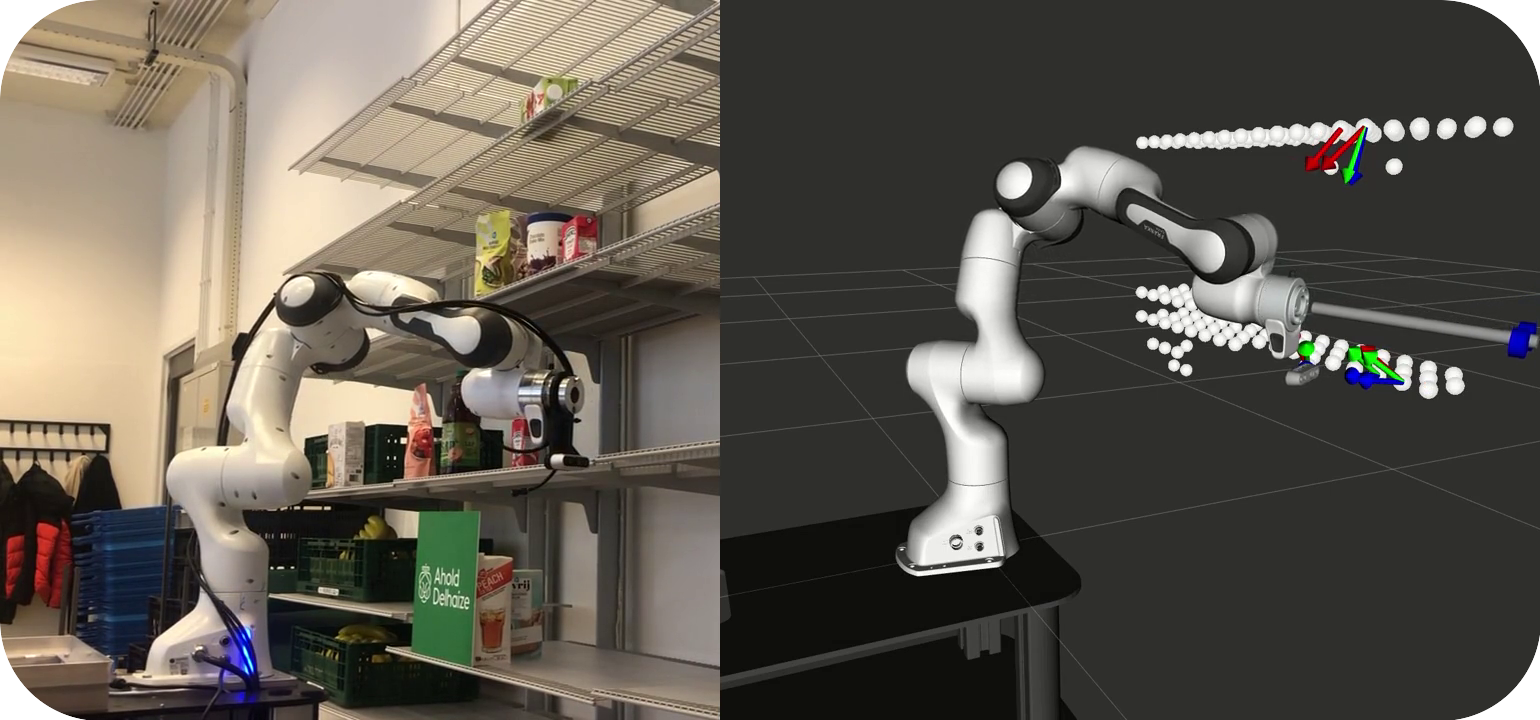
\includegraphics[width=0.95\linewidth]{panda_real/fsd_panda.png}
  \caption{Real robotic manipulator used to run the experiments. A
    Franka Emika Panda is confronted with an unknown shelf
    environment in a supermarket. Arrows indicate the
    normals of the planes obtained by the \ac{fsd}.
    Different colors indicate different links on the robotic
    arm.
  }
  \label{fig:real_panda}
\end{figure}
%
For the Franka Emika Panda, we used the octomap package to
generate the occupancy grid. The method is wrapped into a
ros-node where new control actions are commanded at $40$Hz.
We used three collision links on the robots for collision
avoidance, see \cref{fig:real_panda} for the realization of
\ac{fsd}. The experiments reveal that implicit environment
representations allow for collision-free motion of robotics
arms without the need for a complex perception pipeline.

